\chapter{Research implementation}
\label{chap:implementation}

\section{Data}
\label{sec:data}
This chapter introduces the necessary background information for this study. First, a brief introduction to blockchain technology is provided in \cref{sec:blockchain} and then the concept of \acrfullpl{sc} is introduced in \cref{sec:smart-contract}. Finally, in \cref{sec:smart-contract-vulnerabilities}, the most popular \acrshort{sc} vulnerabilities are described.

\subsection{Smart contract downloader}
\label{sec:smart-contract-downloader}
\url{https://github.com/andstor/smart-contract-downloader}


The largest provider of verified \acrshortpl{sc} is Etherscan. This website provides a list of all verified \acrshortpl{sc} on the blockchain. More on their service...... Etherscan provides a API for downloading verified Smart Contracts. The API is available at \url{https://api.etherscan.io/api}.

In order to download the \acrshortpl{sc} from Etherscan, a tool we need to provide the \acrshortpl{sc} address. The address is the first part of the \acrshortpl{sc} code. The address is the first part of the \acrshortpl{sc} code.

The following code snippet is a Google BigQuery query. It will select all \acrshortpl{sc} addresses on the Ethereum blockchain that has at least one transaction. This query was run on the 1st of April 2022, and the result was downloaded as a CSV file, and is available at \url{https://huggingface.co/datasets/andstor/smart_contracts/blob/main/contract_addresses.csv}. The CSV file is then used to download the \acrshortpl{sc} from Etherscan.

\begin{lstlisting}[
    caption={Google BigQuery query for selecting all \acrlong{sc} addresses on Ethereum that has at least one transaction.},
    label=lst:reentrancy,
    language=SQL]
SELECT contracts.address, COUNT(1) AS tx_count
FROM `bigquery-public-data.crypto_ethereum.contracts` AS contracts
JOIN `bigquery-public-data.crypto_ethereum.transactions` AS transactions 
      ON (transactions.to_address = contracts.address)
GROUP BY contracts.address
ORDER BY tx_count DESC
}
\end{lstlisting}

\todo{Include img of the processing script output}
Saved to file for simple reestarrting, multiprocessing and parallelization.

The total number of files generated by the downloading program was 5,810,042. In order to efficiently process these, all files were combined into a tarfile. A processing script was then created for filtering out all "empty" files. These correspond to a contract address on Ethereum that has not been verified on Etherscan.io. A total of 3,592,350 files were empty, making the source code of 38,17\% of the deployed contracts on Ethereum available. Each non-empty file is then parsed and the contract data is extracted. This extraction process is rather complicated, as smart contract sources come in a wide variety of flavors and formats.

\subsubsection{Normalization}
The most common is a contract written the Solidity language with  a single contract "entry"  \todo{Find a better name for contract keyword}. However, a single contrract file can contain multtiple contracts, making use of properties like inheritance etc.. The source code contracts can also be split over multiple files, a formmat rreefered to as "Multi file". When compiling thtese, the source code files aree "flattened" into a single contract file before compiliattion. Anotther flavour is hte JSON format, which is a language that is used to describe the \acrshortpl{sc}. Here the sourcecode is structured in tthe in the JSON code. Smart contracts can also be vritten in the Vyper language. Vyper is .... \todo{explain vyper}.


\begin{lstlisting}[
    caption={Solidity standard JSON Input format.},
    label=lst:flattened-dataset-cmd,
    language=JSON]
{
    "sources": {/* ... */},
    "settings": {
        "optimizer": {/* ... */},
        "evmVersion": "<VERSION>"
    }
}
\end{lstlisting}

All of the above formats are processed by the processing script, normalizing the contract source code to a single "flattened" contract file. The source code, along with the contract metadata, is then saved across multiple Parquet files, each consisting of 30000 "flattened" contracts. A total of 2,217,692 smart contracts were successfully parsed and normalized.

\subsubsection{Duplication filtering}
\label{sec:duplication-filtering}
A large quantity of Smart Contracts contains duplicated code. Primarily, this is due to the frequent use of library code, such as Safemath and ... \todo{Reference libraries}. Etherscan requires the library code used in a contract to be embedded in the source code. Filtering is applied to produce a dataset with a mostly unique contract source code to mitigate this. This filtering is done by calculating the string distance between the source code. Due to the rather large amount of contracts (\~2 million), the comparison is only made within groups of contracts. These groups are defined by grouping on the "contract\_name" for the \textit{flattened} dataset, and by "file\_name" for the \textit{inflated} dataset. These datasets will be discssed in detail in the following sections.

The actual code filtering is done by applying a token-based similarity algorithm named Jacard Index. The algorithm is computationally efficient and can be used to filter out \acrshortpl{sc} that are not similar to the query. The Jacard Index is a measure of the similarity between two sets. The Jacard Index is defined as the ratio of the size of the intersection to the size of the union of the two sets.


\subsection{Datasets}
\label{sec:datasets}
This section describes the datasets used and created in this study.

\subsubsection{The Pile}
\label{sec:the-pile}
Describe the  PILE...  It consists of among others, a lot of data from GitHub. HHowever, only x\% of the data is smart contracts (Solidity). Hence there is a need for a dataset made up of smart contracts. --> existing datasets....

\begin{figure}[htp]
    \centering
    \includegraphics[width=\textwidth]{figures/Treemap-of-Pile-components-by-effective-size.png}
    \caption{Treemap of Pile components by effective size. SOURCE FROM THEPILE paper}
    \label{fig:flowchart}
\end{figure}


\subsubsection{Verified Smart Contracts}
\label{sec:verified-smart-contracts}
\url{https://github.com/andstor/verified-smart-contracts}
\url{https://huggingface.co/datasets/andstor/smart_contracts}

The Verified Smart Contracts dataset is a dataset consisting of verified Smart Contracts from Etherscan.io. This is real smmart contracts that are deployed to the Ethereum blockchain. A set of 100,000 to 200,000 contracts are provided, containing both Solidity and Vyper code.

\cref{tab:verified-smart-contracts-metrics} shows the metrics of the various (sub)datasets.

\begin{table}
    %\newcolumntype{Y}{>{\centering\arraybackslash}X}
    \def\arraystretch{1.5}
    \small
    \centering
    \caption{Verified Smart Contracts Metrics}
    \label{tab:verified-smart-contracts-metrics}
    \begin{tabularx}{\textwidth}{XXXX}
        \toprule
        \textbf{Component} & \textbf{Size} &  \textbf{Num rows} & \textbf{LoC*}\\
        \midrule
        Raw & 0.80 GiB & 2,217,692 & 839,665,295\\
        Flattened & 1.16 GiB & 136,969 & 97,529,473\\
        Inflated & 0.76 GiB & 186,397 & 53,843,305\\
        Parsed & 4.44 GiB & 4,434,014 & 29,965,185\\
        \bottomrule
    \end{tabularx}
\end{table}

LoC refers to the lines of source\_code. The Parsed dataset counts lines of func\_code + func\_documentation.

\paragraph{Raw}
\label{sec:verified-smart-contracts-raw}
The raw dataset contains mostly the raw data from Etherscan, downloaded with the smart-contract-downlader tool, as described in \cref{sec:smart-contract-downloader}. All different contract formats (JSON, multi-file, etc.) are normalized to a flattened source code structure. 

\todo{Add stats on the raw dataset}

\paragraph{Flattened}
\label{sec:verified-smart-contracts-flattened}

The flattened dataset is a filtered version  of the Raw dataset\cref{sec:verified-smart-contracts-raw}. It contains smart contracts, where every contract contains all required library code. Each "file" is marked in the source code with a comment stating the original file path: //File: path/to/file.sol. These are then filtered for uniqueness with a similarity threshold of 0.9. This means that all contracts whose code shares more than 90\% of the tokens will be discarded. The low uniqueness requirement is due to the often large amount of embedded library code. If the requirement is set to high, the actual contract code will be negligible compared to the library code. Most contracts will be discarded, and the resulting dataset would contain mostly unique library code. However, the dataset as a whole will have a large amount of duplicated libray code. From the 2,217,692 contracts, 2,080,723 duplications are found, giving a duplication percentage of 93.82\%. The resulting dataset consists of 136,969 contracts.

%Processing: 100%|██████| 74/74 [20:22<00:00, 16.51s/it, dupes=2081081/2217692 (93.84%)]

The following command prooduces the flattened dataset:

\lstinline[language=Python]!python script/filter_data.py -s parquet -o data/flattened --threshold 0.9!


\begin{lstlisting}[
    caption={Solidity standard JSON Input format.},
    label=lst:flattened-dataset-cmd,
    language=JSON]
{
  'contract_name': 'MiaKhalifaDAO',
  'contract_address': '0xb3862ca215d5ed2de22734ed001d701adf0a30b4',
  'language': 'Solidity',
  'source_code': '// File: @openzeppelin/contracts/utils/Strings.sol\r\n\r\n\r\n// OpenZeppelin Contracts v4.4.1 (utils/Strings.sol)\r\n\r\npragma solidity ^0.8.0;\r\n\r\n/**\r\n * @dev String operations.\r\n */\r\nlibrary Strings {\r\n...',
  'abi': '[{"inputs":[{"internalType":"uint256","name":"maxBatchSize_","type":"uint256"}...]',
  'compiler_version': 'v0.8.7+commit.e28d00a7',
  'optimization_used': False,
  'runs': 200,
  'constructor_arguments': '000000000000000000000000000000000000000000000000000000000000000a000...',
  'evm_version': 'Default',
  'library': '',
  'license_type': 'MIT',
  'proxy': False,
  'implementation': '',
  'swarm_source': 'ipfs://e490df69bd9ca50e1831a1ac82177e826fee459b0b085a00bd7a727c80d74089'
}
\end{lstlisting}

\begin{figure}[htbp]
    \centering
    %% Creator: Matplotlib, PGF backend
%%
%% To include the figure in your LaTeX document, write
%%   \input{<filename>.pgf}
%%
%% Make sure the required packages are loaded in your preamble
%%   \usepackage{pgf}
%%
%% and, on pdftex
%%   \usepackage[utf8]{inputenc}\DeclareUnicodeCharacter{2212}{-}
%%
%% or, on luatex and xetex
%%   \usepackage{unicode-math}
%%
%% Figures using additional raster images can only be included by \input if
%% they are in the same directory as the main LaTeX file. For loading figures
%% from other directories you can use the `import` package
%%   \usepackage{import}
%%
%% and then include the figures with
%%   \import{<path to file>}{<filename>.pgf}
%%
%% Matplotlib used the following preamble
%%
\begingroup%
\makeatletter%
\begin{pgfpicture}%
\pgfpathrectangle{\pgfpointorigin}{\pgfqpoint{3.378613in}{3.378613in}}%
\pgfusepath{use as bounding box, clip}%
\begin{pgfscope}%
\pgfsetbuttcap%
\pgfsetmiterjoin%
\definecolor{currentfill}{rgb}{1.000000,1.000000,1.000000}%
\pgfsetfillcolor{currentfill}%
\pgfsetlinewidth{0.000000pt}%
\definecolor{currentstroke}{rgb}{1.000000,1.000000,1.000000}%
\pgfsetstrokecolor{currentstroke}%
\pgfsetdash{}{0pt}%
\pgfpathmoveto{\pgfqpoint{0.000000in}{0.000000in}}%
\pgfpathlineto{\pgfqpoint{3.378613in}{0.000000in}}%
\pgfpathlineto{\pgfqpoint{3.378613in}{3.378613in}}%
\pgfpathlineto{\pgfqpoint{0.000000in}{3.378613in}}%
\pgfpathclose%
\pgfusepath{fill}%
\end{pgfscope}%
\begin{pgfscope}%
\pgfsetbuttcap%
\pgfsetmiterjoin%
\definecolor{currentfill}{rgb}{0.925882,1.000000,0.634902}%
\pgfsetfillcolor{currentfill}%
\pgfsetfillopacity{0.700000}%
\pgfsetlinewidth{0.000000pt}%
\definecolor{currentstroke}{rgb}{0.000000,0.000000,0.000000}%
\pgfsetstrokecolor{currentstroke}%
\pgfsetstrokeopacity{0.700000}%
\pgfsetdash{}{0pt}%
\pgfpathmoveto{\pgfqpoint{2.751880in}{1.697753in}}%
\pgfpathcurveto{\pgfqpoint{2.751880in}{1.710594in}}{\pgfqpoint{2.751638in}{1.723433in}}{\pgfqpoint{2.751153in}{1.736265in}}%
\pgfpathcurveto{\pgfqpoint{2.750668in}{1.749097in}}{\pgfqpoint{2.749941in}{1.761918in}}{\pgfqpoint{2.748973in}{1.774723in}}%
\pgfpathlineto{\pgfqpoint{2.240256in}{1.736238in}}%
\pgfpathcurveto{\pgfqpoint{2.240740in}{1.729836in}}{\pgfqpoint{2.241104in}{1.723425in}}{\pgfqpoint{2.241346in}{1.717009in}}%
\pgfpathcurveto{\pgfqpoint{2.241588in}{1.710593in}}{\pgfqpoint{2.241709in}{1.704173in}}{\pgfqpoint{2.241709in}{1.697753in}}%
\pgfpathlineto{\pgfqpoint{2.751880in}{1.697753in}}%
\pgfpathclose%
\pgfusepath{fill}%
\end{pgfscope}%
\begin{pgfscope}%
\pgfsetbuttcap%
\pgfsetmiterjoin%
\definecolor{currentfill}{rgb}{0.882745,0.000000,0.111414}%
\pgfsetfillcolor{currentfill}%
\pgfsetfillopacity{0.700000}%
\pgfsetlinewidth{0.000000pt}%
\definecolor{currentstroke}{rgb}{0.000000,0.000000,0.000000}%
\pgfsetstrokecolor{currentstroke}%
\pgfsetstrokeopacity{0.700000}%
\pgfsetdash{}{0pt}%
\pgfpathmoveto{\pgfqpoint{2.748973in}{1.774723in}}%
\pgfpathcurveto{\pgfqpoint{2.735160in}{1.957309in}}{\pgfqpoint{2.672448in}{2.132855in}}{\pgfqpoint{2.567445in}{2.282865in}}%
\pgfpathcurveto{\pgfqpoint{2.462442in}{2.432875in}}{\pgfqpoint{2.318970in}{2.551890in}}{\pgfqpoint{2.152142in}{2.627370in}}%
\pgfpathcurveto{\pgfqpoint{1.985315in}{2.702851in}}{\pgfqpoint{1.801205in}{2.732050in}}{\pgfqpoint{1.619210in}{2.711892in}}%
\pgfpathcurveto{\pgfqpoint{1.437215in}{2.691734in}}{\pgfqpoint{1.263958in}{2.622951in}}{\pgfqpoint{1.117692in}{2.512792in}}%
\pgfpathcurveto{\pgfqpoint{0.971427in}{2.402632in}}{\pgfqpoint{0.857477in}{2.255104in}}{\pgfqpoint{0.787848in}{2.085752in}}%
\pgfpathcurveto{\pgfqpoint{0.718218in}{1.916399in}}{\pgfqpoint{0.695444in}{1.731384in}}{\pgfqpoint{0.721923in}{1.550201in}}%
\pgfpathcurveto{\pgfqpoint{0.748403in}{1.369017in}}{\pgfqpoint{0.823172in}{1.198259in}}{\pgfqpoint{0.938355in}{1.055916in}}%
\pgfpathcurveto{\pgfqpoint{1.053538in}{0.913572in}}{\pgfqpoint{1.204942in}{0.804825in}}{\pgfqpoint{1.376615in}{0.741131in}}%
\pgfpathlineto{\pgfqpoint{1.554077in}{1.219442in}}%
\pgfpathcurveto{\pgfqpoint{1.468240in}{1.251289in}}{\pgfqpoint{1.392538in}{1.305663in}}{\pgfqpoint{1.334947in}{1.376834in}}%
\pgfpathcurveto{\pgfqpoint{1.277356in}{1.448006in}}{\pgfqpoint{1.239971in}{1.533385in}}{\pgfqpoint{1.226731in}{1.623977in}}%
\pgfpathcurveto{\pgfqpoint{1.213491in}{1.714569in}}{\pgfqpoint{1.224879in}{1.807076in}}{\pgfqpoint{1.259693in}{1.891752in}}%
\pgfpathcurveto{\pgfqpoint{1.294508in}{1.976429in}}{\pgfqpoint{1.351483in}{2.050192in}}{\pgfqpoint{1.424616in}{2.105272in}}%
\pgfpathcurveto{\pgfqpoint{1.497748in}{2.160352in}}{\pgfqpoint{1.584377in}{2.194743in}}{\pgfqpoint{1.675374in}{2.204822in}}%
\pgfpathcurveto{\pgfqpoint{1.766372in}{2.214902in}}{\pgfqpoint{1.858427in}{2.200302in}}{\pgfqpoint{1.941841in}{2.162562in}}%
\pgfpathcurveto{\pgfqpoint{2.025254in}{2.124821in}}{\pgfqpoint{2.096991in}{2.065314in}}{\pgfqpoint{2.149492in}{1.990309in}}%
\pgfpathcurveto{\pgfqpoint{2.201994in}{1.915304in}}{\pgfqpoint{2.233349in}{1.827531in}}{\pgfqpoint{2.240256in}{1.736238in}}%
\pgfpathlineto{\pgfqpoint{2.748973in}{1.774723in}}%
\pgfpathclose%
\pgfusepath{fill}%
\end{pgfscope}%
\begin{pgfscope}%
\pgfsetbuttcap%
\pgfsetmiterjoin%
\definecolor{currentfill}{rgb}{0.000000,0.786667,0.312353}%
\pgfsetfillcolor{currentfill}%
\pgfsetfillopacity{0.700000}%
\pgfsetlinewidth{0.000000pt}%
\definecolor{currentstroke}{rgb}{0.000000,0.000000,0.000000}%
\pgfsetstrokecolor{currentstroke}%
\pgfsetstrokeopacity{0.700000}%
\pgfsetdash{}{0pt}%
\pgfpathmoveto{\pgfqpoint{1.376615in}{0.741131in}}%
\pgfpathcurveto{\pgfqpoint{1.391448in}{0.735628in}}{\pgfqpoint{1.406407in}{0.730470in}}{\pgfqpoint{1.421480in}{0.725663in}}%
\pgfpathcurveto{\pgfqpoint{1.436553in}{0.720855in}}{\pgfqpoint{1.451736in}{0.716398in}}{\pgfqpoint{1.467016in}{0.712297in}}%
\pgfpathlineto{\pgfqpoint{1.599278in}{1.205025in}}%
\pgfpathcurveto{\pgfqpoint{1.591638in}{1.207076in}}{\pgfqpoint{1.584046in}{1.209304in}}{\pgfqpoint{1.576510in}{1.211708in}}%
\pgfpathcurveto{\pgfqpoint{1.568973in}{1.214112in}}{\pgfqpoint{1.561494in}{1.216690in}}{\pgfqpoint{1.554077in}{1.219442in}}%
\pgfpathlineto{\pgfqpoint{1.376615in}{0.741131in}}%
\pgfpathclose%
\pgfusepath{fill}%
\end{pgfscope}%
\begin{pgfscope}%
\pgfsetbuttcap%
\pgfsetmiterjoin%
\definecolor{currentfill}{rgb}{0.930307,0.285685,0.029301}%
\pgfsetfillcolor{currentfill}%
\pgfsetfillopacity{0.700000}%
\pgfsetlinewidth{0.000000pt}%
\definecolor{currentstroke}{rgb}{0.000000,0.000000,0.000000}%
\pgfsetstrokecolor{currentstroke}%
\pgfsetstrokeopacity{0.700000}%
\pgfsetdash{}{0pt}%
\pgfpathmoveto{\pgfqpoint{1.467016in}{0.712297in}}%
\pgfpathcurveto{\pgfqpoint{1.642990in}{0.665061in}}{\pgfqpoint{1.828446in}{0.665812in}}{\pgfqpoint{2.004032in}{0.714471in}}%
\pgfpathcurveto{\pgfqpoint{2.179617in}{0.763130in}}{\pgfqpoint{2.339006in}{0.857944in}}{\pgfqpoint{2.465565in}{0.989020in}}%
\pgfpathlineto{\pgfqpoint{2.098552in}{1.343386in}}%
\pgfpathcurveto{\pgfqpoint{2.035272in}{1.277849in}}{\pgfqpoint{1.955578in}{1.230441in}}{\pgfqpoint{1.867785in}{1.206112in}}%
\pgfpathcurveto{\pgfqpoint{1.779992in}{1.181782in}}{\pgfqpoint{1.687265in}{1.181407in}}{\pgfqpoint{1.599278in}{1.205025in}}%
\pgfpathlineto{\pgfqpoint{1.467016in}{0.712297in}}%
\pgfpathclose%
\pgfusepath{fill}%
\end{pgfscope}%
\begin{pgfscope}%
\pgfsetbuttcap%
\pgfsetmiterjoin%
\definecolor{currentfill}{rgb}{0.063700,0.382199,0.851986}%
\pgfsetfillcolor{currentfill}%
\pgfsetfillopacity{0.700000}%
\pgfsetlinewidth{0.000000pt}%
\definecolor{currentstroke}{rgb}{0.000000,0.000000,0.000000}%
\pgfsetstrokecolor{currentstroke}%
\pgfsetstrokeopacity{0.700000}%
\pgfsetdash{}{0pt}%
\pgfpathmoveto{\pgfqpoint{2.465565in}{0.989020in}}%
\pgfpathcurveto{\pgfqpoint{2.556545in}{1.083247in}}{\pgfqpoint{2.628535in}{1.194117in}}{\pgfqpoint{2.677597in}{1.315562in}}%
\pgfpathcurveto{\pgfqpoint{2.726659in}{1.437008in}}{\pgfqpoint{2.751880in}{1.566772in}}{\pgfqpoint{2.751880in}{1.697753in}}%
\pgfpathlineto{\pgfqpoint{2.241709in}{1.697753in}}%
\pgfpathcurveto{\pgfqpoint{2.241709in}{1.632262in}}{\pgfqpoint{2.229099in}{1.567380in}}{\pgfqpoint{2.204568in}{1.506658in}}%
\pgfpathcurveto{\pgfqpoint{2.180037in}{1.445935in}}{\pgfqpoint{2.144042in}{1.390500in}}{\pgfqpoint{2.098552in}{1.343386in}}%
\pgfpathlineto{\pgfqpoint{2.465565in}{0.989020in}}%
\pgfpathclose%
\pgfusepath{fill}%
\end{pgfscope}%
\begin{pgfscope}%
\pgfsetbuttcap%
\pgfsetmiterjoin%
\definecolor{currentfill}{rgb}{0.925882,1.000000,0.634902}%
\pgfsetfillcolor{currentfill}%
\pgfsetfillopacity{0.700000}%
\pgfsetlinewidth{0.000000pt}%
\definecolor{currentstroke}{rgb}{0.000000,0.000000,0.000000}%
\pgfsetstrokecolor{currentstroke}%
\pgfsetstrokeopacity{0.700000}%
\pgfsetdash{}{0pt}%
\pgfpathmoveto{\pgfqpoint{3.262050in}{1.697753in}}%
\pgfpathcurveto{\pgfqpoint{3.262050in}{1.717014in}}{\pgfqpoint{3.261687in}{1.736274in}}{\pgfqpoint{3.260960in}{1.755521in}}%
\pgfpathcurveto{\pgfqpoint{3.260233in}{1.774769in}}{\pgfqpoint{3.259143in}{1.794001in}}{\pgfqpoint{3.257690in}{1.813207in}}%
\pgfpathlineto{\pgfqpoint{2.748973in}{1.774723in}}%
\pgfpathcurveto{\pgfqpoint{2.749941in}{1.761918in}}{\pgfqpoint{2.750668in}{1.749097in}}{\pgfqpoint{2.751153in}{1.736265in}}%
\pgfpathcurveto{\pgfqpoint{2.751638in}{1.723433in}}{\pgfqpoint{2.751880in}{1.710594in}}{\pgfqpoint{2.751880in}{1.697753in}}%
\pgfpathlineto{\pgfqpoint{3.262050in}{1.697753in}}%
\pgfpathclose%
\pgfusepath{fill}%
\end{pgfscope}%
\begin{pgfscope}%
\pgfsetbuttcap%
\pgfsetmiterjoin%
\definecolor{currentfill}{rgb}{0.882745,0.000000,0.111414}%
\pgfsetfillcolor{currentfill}%
\pgfsetfillopacity{0.700000}%
\pgfsetlinewidth{0.000000pt}%
\definecolor{currentstroke}{rgb}{0.000000,0.000000,0.000000}%
\pgfsetstrokecolor{currentstroke}%
\pgfsetstrokeopacity{0.700000}%
\pgfsetdash{}{0pt}%
\pgfpathmoveto{\pgfqpoint{3.257690in}{1.813207in}}%
\pgfpathcurveto{\pgfqpoint{3.252513in}{1.881632in}}{\pgfqpoint{3.242741in}{1.949631in}}{\pgfqpoint{3.228439in}{2.016745in}}%
\pgfpathcurveto{\pgfqpoint{3.214137in}{2.083858in}}{\pgfqpoint{3.195338in}{2.149933in}}{\pgfqpoint{3.172168in}{2.214524in}}%
\pgfpathlineto{\pgfqpoint{2.691959in}{2.042267in}}%
\pgfpathcurveto{\pgfqpoint{2.707405in}{1.999207in}}{\pgfqpoint{2.719938in}{1.955156in}}{\pgfqpoint{2.729472in}{1.910414in}}%
\pgfpathcurveto{\pgfqpoint{2.739007in}{1.865672in}}{\pgfqpoint{2.745522in}{1.820339in}}{\pgfqpoint{2.748973in}{1.774723in}}%
\pgfpathlineto{\pgfqpoint{3.257690in}{1.813207in}}%
\pgfpathclose%
\pgfusepath{fill}%
\end{pgfscope}%
\begin{pgfscope}%
\pgfsetbuttcap%
\pgfsetmiterjoin%
\definecolor{currentfill}{rgb}{0.917292,0.307374,0.323876}%
\pgfsetfillcolor{currentfill}%
\pgfsetfillopacity{0.700000}%
\pgfsetlinewidth{0.000000pt}%
\definecolor{currentstroke}{rgb}{0.000000,0.000000,0.000000}%
\pgfsetstrokecolor{currentstroke}%
\pgfsetstrokeopacity{0.700000}%
\pgfsetdash{}{0pt}%
\pgfpathmoveto{\pgfqpoint{3.172168in}{2.214524in}}%
\pgfpathcurveto{\pgfqpoint{3.143867in}{2.293420in}}{\pgfqpoint{3.109133in}{2.369858in}}{\pgfqpoint{3.068316in}{2.443066in}}%
\pgfpathcurveto{\pgfqpoint{3.027499in}{2.516275in}}{\pgfqpoint{2.980737in}{2.586007in}}{\pgfqpoint{2.928502in}{2.651558in}}%
\pgfpathlineto{\pgfqpoint{2.529514in}{2.333623in}}%
\pgfpathcurveto{\pgfqpoint{2.564338in}{2.289922in}}{\pgfqpoint{2.595512in}{2.243434in}}{\pgfqpoint{2.622724in}{2.194628in}}%
\pgfpathcurveto{\pgfqpoint{2.649935in}{2.145823in}}{\pgfqpoint{2.673091in}{2.094864in}}{\pgfqpoint{2.691959in}{2.042267in}}%
\pgfpathlineto{\pgfqpoint{3.172168in}{2.214524in}}%
\pgfpathclose%
\pgfusepath{fill}%
\end{pgfscope}%
\begin{pgfscope}%
\pgfsetbuttcap%
\pgfsetmiterjoin%
\definecolor{currentfill}{rgb}{0.989063,0.592703,0.504860}%
\pgfsetfillcolor{currentfill}%
\pgfsetfillopacity{0.700000}%
\pgfsetlinewidth{0.000000pt}%
\definecolor{currentstroke}{rgb}{0.000000,0.000000,0.000000}%
\pgfsetstrokecolor{currentstroke}%
\pgfsetstrokeopacity{0.700000}%
\pgfsetdash{}{0pt}%
\pgfpathmoveto{\pgfqpoint{2.928502in}{2.651558in}}%
\pgfpathcurveto{\pgfqpoint{2.784634in}{2.832104in}}{\pgfqpoint{2.601763in}{2.977780in}}{\pgfqpoint{2.393626in}{3.077647in}}%
\pgfpathcurveto{\pgfqpoint{2.185488in}{3.177513in}}{\pgfqpoint{1.957427in}{3.229006in}}{\pgfqpoint{1.726572in}{3.228256in}}%
\pgfpathlineto{\pgfqpoint{1.728227in}{2.718088in}}%
\pgfpathcurveto{\pgfqpoint{1.882131in}{2.718588in}}{\pgfqpoint{2.034171in}{2.684260in}}{\pgfqpoint{2.172930in}{2.617682in}}%
\pgfpathcurveto{\pgfqpoint{2.311689in}{2.551104in}}{\pgfqpoint{2.433602in}{2.453987in}}{\pgfqpoint{2.529514in}{2.333623in}}%
\pgfpathlineto{\pgfqpoint{2.928502in}{2.651558in}}%
\pgfpathclose%
\pgfusepath{fill}%
\end{pgfscope}%
\begin{pgfscope}%
\pgfsetbuttcap%
\pgfsetmiterjoin%
\definecolor{currentfill}{rgb}{0.991894,0.815723,0.745126}%
\pgfsetfillcolor{currentfill}%
\pgfsetfillopacity{0.700000}%
\pgfsetlinewidth{0.000000pt}%
\definecolor{currentstroke}{rgb}{0.000000,0.000000,0.000000}%
\pgfsetstrokecolor{currentstroke}%
\pgfsetstrokeopacity{0.700000}%
\pgfsetdash{}{0pt}%
\pgfpathmoveto{\pgfqpoint{1.726572in}{3.228256in}}%
\pgfpathcurveto{\pgfqpoint{1.368074in}{3.227093in}}{\pgfqpoint{1.021135in}{3.100006in}}{\pgfqpoint{0.746712in}{2.869325in}}%
\pgfpathcurveto{\pgfqpoint{0.472288in}{2.638643in}}{\pgfqpoint{0.287451in}{2.318718in}}{\pgfqpoint{0.224675in}{1.965757in}}%
\pgfpathcurveto{\pgfqpoint{0.161899in}{1.612796in}}{\pgfqpoint{0.225089in}{1.248757in}}{\pgfqpoint{0.403144in}{0.937600in}}%
\pgfpathcurveto{\pgfqpoint{0.581199in}{0.626443in}}{\pgfqpoint{0.863041in}{0.387524in}}{\pgfqpoint{1.199153in}{0.262821in}}%
\pgfpathlineto{\pgfqpoint{1.376615in}{0.741131in}}%
\pgfpathcurveto{\pgfqpoint{1.152540in}{0.824267in}}{\pgfqpoint{0.964645in}{0.983546in}}{\pgfqpoint{0.845942in}{1.190984in}}%
\pgfpathcurveto{\pgfqpoint{0.727239in}{1.398422in}}{\pgfqpoint{0.685112in}{1.641115in}}{\pgfqpoint{0.726963in}{1.876422in}}%
\pgfpathcurveto{\pgfqpoint{0.768814in}{2.111729in}}{\pgfqpoint{0.892038in}{2.325013in}}{\pgfqpoint{1.074987in}{2.478801in}}%
\pgfpathcurveto{\pgfqpoint{1.257936in}{2.632588in}}{\pgfqpoint{1.489229in}{2.717313in}}{\pgfqpoint{1.728227in}{2.718088in}}%
\pgfpathlineto{\pgfqpoint{1.726572in}{3.228256in}}%
\pgfpathclose%
\pgfusepath{fill}%
\end{pgfscope}%
\begin{pgfscope}%
\pgfsetbuttcap%
\pgfsetmiterjoin%
\definecolor{currentfill}{rgb}{0.000000,0.786667,0.312353}%
\pgfsetfillcolor{currentfill}%
\pgfsetfillopacity{0.700000}%
\pgfsetlinewidth{0.000000pt}%
\definecolor{currentstroke}{rgb}{0.000000,0.000000,0.000000}%
\pgfsetstrokecolor{currentstroke}%
\pgfsetstrokeopacity{0.700000}%
\pgfsetdash{}{0pt}%
\pgfpathmoveto{\pgfqpoint{1.199153in}{0.262821in}}%
\pgfpathcurveto{\pgfqpoint{1.221403in}{0.254566in}}{\pgfqpoint{1.243841in}{0.246829in}}{\pgfqpoint{1.266451in}{0.239618in}}%
\pgfpathcurveto{\pgfqpoint{1.289060in}{0.232406in}}{\pgfqpoint{1.311835in}{0.225721in}}{\pgfqpoint{1.334755in}{0.219569in}}%
\pgfpathlineto{\pgfqpoint{1.467016in}{0.712297in}}%
\pgfpathcurveto{\pgfqpoint{1.451736in}{0.716398in}}{\pgfqpoint{1.436553in}{0.720855in}}{\pgfqpoint{1.421480in}{0.725663in}}%
\pgfpathcurveto{\pgfqpoint{1.406407in}{0.730470in}}{\pgfqpoint{1.391448in}{0.735628in}}{\pgfqpoint{1.376615in}{0.741131in}}%
\pgfpathlineto{\pgfqpoint{1.199153in}{0.262821in}}%
\pgfpathclose%
\pgfusepath{fill}%
\end{pgfscope}%
\begin{pgfscope}%
\pgfsetbuttcap%
\pgfsetmiterjoin%
\definecolor{currentfill}{rgb}{0.930307,0.285685,0.029301}%
\pgfsetfillcolor{currentfill}%
\pgfsetfillopacity{0.700000}%
\pgfsetlinewidth{0.000000pt}%
\definecolor{currentstroke}{rgb}{0.000000,0.000000,0.000000}%
\pgfsetstrokecolor{currentstroke}%
\pgfsetstrokeopacity{0.700000}%
\pgfsetdash{}{0pt}%
\pgfpathmoveto{\pgfqpoint{1.334755in}{0.219569in}}%
\pgfpathcurveto{\pgfqpoint{1.475152in}{0.181883in}}{\pgfqpoint{1.620204in}{0.164390in}}{\pgfqpoint{1.765535in}{0.167619in}}%
\pgfpathcurveto{\pgfqpoint{1.910866in}{0.170848in}}{\pgfqpoint{2.054998in}{0.194765in}}{\pgfqpoint{2.193582in}{0.238650in}}%
\pgfpathlineto{\pgfqpoint{2.039568in}{0.725018in}}%
\pgfpathcurveto{\pgfqpoint{1.947178in}{0.695761in}}{\pgfqpoint{1.851090in}{0.679816in}}{\pgfqpoint{1.754203in}{0.677664in}}%
\pgfpathcurveto{\pgfqpoint{1.657316in}{0.675511in}}{\pgfqpoint{1.560614in}{0.687173in}}{\pgfqpoint{1.467016in}{0.712297in}}%
\pgfpathlineto{\pgfqpoint{1.334755in}{0.219569in}}%
\pgfpathclose%
\pgfusepath{fill}%
\end{pgfscope}%
\begin{pgfscope}%
\pgfsetbuttcap%
\pgfsetmiterjoin%
\definecolor{currentfill}{rgb}{0.995815,0.464325,0.203521}%
\pgfsetfillcolor{currentfill}%
\pgfsetfillopacity{0.700000}%
\pgfsetlinewidth{0.000000pt}%
\definecolor{currentstroke}{rgb}{0.000000,0.000000,0.000000}%
\pgfsetstrokecolor{currentstroke}%
\pgfsetstrokeopacity{0.700000}%
\pgfsetdash{}{0pt}%
\pgfpathmoveto{\pgfqpoint{2.193582in}{0.238650in}}%
\pgfpathcurveto{\pgfqpoint{2.314418in}{0.276914in}}{\pgfqpoint{2.430034in}{0.330041in}}{\pgfqpoint{2.537772in}{0.396809in}}%
\pgfpathcurveto{\pgfqpoint{2.645509in}{0.463577in}}{\pgfqpoint{2.744537in}{0.543471in}}{\pgfqpoint{2.832577in}{0.634654in}}%
\pgfpathlineto{\pgfqpoint{2.465565in}{0.989020in}}%
\pgfpathcurveto{\pgfqpoint{2.406871in}{0.928232in}}{\pgfqpoint{2.340853in}{0.874969in}}{\pgfqpoint{2.269027in}{0.830457in}}%
\pgfpathcurveto{\pgfqpoint{2.197202in}{0.785945in}}{\pgfqpoint{2.120125in}{0.750527in}}{\pgfqpoint{2.039568in}{0.725018in}}%
\pgfpathlineto{\pgfqpoint{2.193582in}{0.238650in}}%
\pgfpathclose%
\pgfusepath{fill}%
\end{pgfscope}%
\begin{pgfscope}%
\pgfsetbuttcap%
\pgfsetmiterjoin%
\definecolor{currentfill}{rgb}{0.063700,0.382199,0.851986}%
\pgfsetfillcolor{currentfill}%
\pgfsetfillopacity{0.700000}%
\pgfsetlinewidth{0.000000pt}%
\definecolor{currentstroke}{rgb}{0.000000,0.000000,0.000000}%
\pgfsetstrokecolor{currentstroke}%
\pgfsetstrokeopacity{0.700000}%
\pgfsetdash{}{0pt}%
\pgfpathmoveto{\pgfqpoint{2.832577in}{0.634654in}}%
\pgfpathcurveto{\pgfqpoint{2.969047in}{0.775994in}}{\pgfqpoint{3.077034in}{0.942299in}}{\pgfqpoint{3.150626in}{1.124467in}}%
\pgfpathcurveto{\pgfqpoint{3.224219in}{1.306635in}}{\pgfqpoint{3.262050in}{1.501281in}}{\pgfqpoint{3.262050in}{1.697753in}}%
\pgfpathlineto{\pgfqpoint{2.751880in}{1.697753in}}%
\pgfpathcurveto{\pgfqpoint{2.751880in}{1.566772in}}{\pgfqpoint{2.726659in}{1.437008in}}{\pgfqpoint{2.677597in}{1.315562in}}%
\pgfpathcurveto{\pgfqpoint{2.628535in}{1.194117in}}{\pgfqpoint{2.556545in}{1.083247in}}{\pgfqpoint{2.465565in}{0.989020in}}%
\pgfpathlineto{\pgfqpoint{2.832577in}{0.634654in}}%
\pgfpathclose%
\pgfusepath{fill}%
\end{pgfscope}%
\begin{pgfscope}%
\definecolor{textcolor}{rgb}{0.000000,0.000000,0.000000}%
\pgfsetstrokecolor{textcolor}%
\pgfsetfillcolor{textcolor}%
\pgftext[x=2.445269in,y=1.724711in,left,]{\color{textcolor}\rmfamily\fontsize{9.000000}{10.800000}\selectfont E}%
\end{pgfscope}%
\begin{pgfscope}%
\definecolor{textcolor}{rgb}{0.000000,0.000000,0.000000}%
\pgfsetstrokecolor{textcolor}%
\pgfsetfillcolor{textcolor}%
\pgftext[x=1.301846in,y=2.268280in,right,]{\color{textcolor}\rmfamily\fontsize{9.000000}{10.800000}\selectfont H}%
\end{pgfscope}%
\begin{pgfscope}%
\definecolor{textcolor}{rgb}{0.000000,0.000000,0.000000}%
\pgfsetstrokecolor{textcolor}%
\pgfsetfillcolor{textcolor}%
\pgftext[x=1.514498in,y=1.017290in,right,]{\color{textcolor}\rmfamily\fontsize{9.000000}{10.800000}\selectfont L}%
\end{pgfscope}%
\begin{pgfscope}%
\definecolor{textcolor}{rgb}{0.000000,0.000000,0.000000}%
\pgfsetstrokecolor{textcolor}%
\pgfsetfillcolor{textcolor}%
\pgftext[x=1.922284in,y=1.009455in,left,]{\color{textcolor}\rmfamily\fontsize{9.000000}{10.800000}\selectfont M}%
\end{pgfscope}%
\begin{pgfscope}%
\definecolor{textcolor}{rgb}{0.000000,0.000000,0.000000}%
\pgfsetstrokecolor{textcolor}%
\pgfsetfillcolor{textcolor}%
\pgftext[x=2.393780in,y=1.430219in,left,]{\color{textcolor}\rmfamily\fontsize{9.000000}{10.800000}\selectfont S}%
\end{pgfscope}%
\begin{pgfscope}%
\definecolor{textcolor}{rgb}{0.000000,0.000000,0.000000}%
\pgfsetstrokecolor{textcolor}%
\pgfsetfillcolor{textcolor}%
\pgftext[x=2.938082in,y=1.743326in,left,]{\color{textcolor}\rmfamily\fontsize{9.000000}{10.800000}\selectfont E}%
\end{pgfscope}%
\begin{pgfscope}%
\definecolor{textcolor}{rgb}{0.000000,0.000000,0.000000}%
\pgfsetstrokecolor{textcolor}%
\pgfsetfillcolor{textcolor}%
\pgftext[x=2.912427in,y=1.949402in,left,]{\color{textcolor}\rmfamily\fontsize{9.000000}{10.800000}\selectfont H}%
\end{pgfscope}%
\begin{pgfscope}%
\definecolor{textcolor}{rgb}{0.000000,0.000000,0.000000}%
\pgfsetstrokecolor{textcolor}%
\pgfsetfillcolor{textcolor}%
\pgftext[x=2.786108in,y=2.285722in,left,]{\color{textcolor}\rmfamily\fontsize{9.000000}{10.800000}\selectfont HL}%
\end{pgfscope}%
\begin{pgfscope}%
\definecolor{textcolor}{rgb}{0.000000,0.000000,0.000000}%
\pgfsetstrokecolor{textcolor}%
\pgfsetfillcolor{textcolor}%
\pgftext[x=2.253852in,y=2.786336in,left,]{\color{textcolor}\rmfamily\fontsize{9.000000}{10.800000}\selectfont HM}%
\end{pgfscope}%
\begin{pgfscope}%
\definecolor{textcolor}{rgb}{0.000000,0.000000,0.000000}%
\pgfsetstrokecolor{textcolor}%
\pgfsetfillcolor{textcolor}%
\pgftext[x=0.542791in,y=1.909178in,right,]{\color{textcolor}\rmfamily\fontsize{9.000000}{10.800000}\selectfont HML}%
\end{pgfscope}%
\begin{pgfscope}%
\definecolor{textcolor}{rgb}{0.000000,0.000000,0.000000}%
\pgfsetstrokecolor{textcolor}%
\pgfsetfillcolor{textcolor}%
\pgftext[x=1.364636in,y=0.547446in,right,]{\color{textcolor}\rmfamily\fontsize{9.000000}{10.800000}\selectfont L}%
\end{pgfscope}%
\begin{pgfscope}%
\definecolor{textcolor}{rgb}{0.000000,0.000000,0.000000}%
\pgfsetstrokecolor{textcolor}%
\pgfsetfillcolor{textcolor}%
\pgftext[x=1.758358in,y=0.490647in,left,]{\color{textcolor}\rmfamily\fontsize{9.000000}{10.800000}\selectfont M}%
\end{pgfscope}%
\begin{pgfscope}%
\definecolor{textcolor}{rgb}{0.000000,0.000000,0.000000}%
\pgfsetstrokecolor{textcolor}%
\pgfsetfillcolor{textcolor}%
\pgftext[x=2.367567in,y=0.671453in,left,]{\color{textcolor}\rmfamily\fontsize{9.000000}{10.800000}\selectfont ML}%
\end{pgfscope}%
\begin{pgfscope}%
\definecolor{textcolor}{rgb}{0.000000,0.000000,0.000000}%
\pgfsetstrokecolor{textcolor}%
\pgfsetfillcolor{textcolor}%
\pgftext[x=2.851041in,y=1.245494in,left,]{\color{textcolor}\rmfamily\fontsize{9.000000}{10.800000}\selectfont S}%
\end{pgfscope}%
\end{pgfpicture}%
\makeatother%
\endgroup%

    \caption{Doughnut chart over the distribution of the vulnerability severities in the flattened dataset at different granularity levels, where each level occurs at least once in the \acrshort{sc}. The outer ring shows the additional security levels for each contract. For example, "HML" means that the contract has at least three vulnerabilities with the corresponding "High", "Medium", and "Low" security levels.}
\end{figure}


\begin{figure}[htbp]
    \centering
    \input{figures/flattened_vulnerabilities_bar.pgf}
    \caption{Distribution of vulnerabilities in the flattened dataset.}
\end{figure}

\paragraph{Inflated}
\label{sec:verified-smart-contracts-inflated}
The inflated dataset is also based on the raw dataset. Each contract file in the dataset is split into its original representative files. This mitigates a lot of the problems of the flattened dataset in terms of duplicated library code. The library code would, along with other imported contract files, be split into separate contract records. The 2,217,692 "raw" smart contracts are inflated to a total of 5,403,136 separate contract files. These are then grouped by "file\_name" and filtered for uniqueness with a similarity threshold of 0.9. This should produce a dataset with a large amount of unique source code, with low quantities of library code. A total of 5,216,739 duplications are found, giving a duplication percentage of 96.56\%. The resulting dataset consists of 186,397 contracts.

%Processing: 100%|██████| 74/74 [22:50<00:00, 18.52s/it, dupes=5217191/5403136 (96.56%)]


\lstinline[language=Python]!python script/filter_data.py -s parquet -o data/inflated --split-files --threshold 0.9!
dupes=5217191/5403136 (96.56%)


\begin{lstlisting}[
    caption={Solidity standard JSON Input format.},
    label=lst:flattened-dataset-cmd,
    language=JSON]
    {
        'contract_name': 'PinkLemonade',
        'file_path': 'PinkLemonade.sol',
        'contract_address': '0x9a5be3cc368f01a0566a613aad7183783cff7eec',
        'language': 'Solidity',
        'source_code': '/**\r\n\r\nt.me/pinklemonadecoin\r\n*/\r\n\r\n// SPDX-License-Identifier: MIT\r\npragma solidity ^0.8.0;\r\n\r\n\r\n/*\r\n * @dev Provides information about the current execution context, including the\r\n * sender of the transaction and its data. While these are generally available...',
        'abi': '[{"inputs":[],"stateMutability":"nonpayable","type":"constructor"}...]',
        'compiler_version': 'v0.8.4+commit.c7e474f2',
        'optimization_used': False,
        'runs': 200,
        'constructor_arguments': '',
        'evm_version': 'Default',
        'library': '',
        'license_type': 'MIT',
        'proxy': False,
        'implementation': '',
        'swarm_source': 'ipfs://eb0ac9491a04e7a196280fd27ce355a85d79b34c7b0a83ab606d27972a06050c'
      }
      
      
\end{lstlisting}

\begin{figure}[htbp]
    \centering
    %% Creator: Matplotlib, PGF backend
%%
%% To include the figure in your LaTeX document, write
%%   \input{<filename>.pgf}
%%
%% Make sure the required packages are loaded in your preamble
%%   \usepackage{pgf}
%%
%% and, on pdftex
%%   \usepackage[utf8]{inputenc}\DeclareUnicodeCharacter{2212}{-}
%%
%% or, on luatex and xetex
%%   \usepackage{unicode-math}
%%
%% Figures using additional raster images can only be included by \input if
%% they are in the same directory as the main LaTeX file. For loading figures
%% from other directories you can use the `import` package
%%   \usepackage{import}
%%
%% and then include the figures with
%%   \import{<path to file>}{<filename>.pgf}
%%
%% Matplotlib used the following preamble
%%
\begingroup%
\makeatletter%
\begin{pgfpicture}%
\pgfpathrectangle{\pgfpointorigin}{\pgfqpoint{3.465474in}{3.767802in}}%
\pgfusepath{use as bounding box, clip}%
\begin{pgfscope}%
\pgfsetbuttcap%
\pgfsetmiterjoin%
\definecolor{currentfill}{rgb}{1.000000,1.000000,1.000000}%
\pgfsetfillcolor{currentfill}%
\pgfsetlinewidth{0.000000pt}%
\definecolor{currentstroke}{rgb}{1.000000,1.000000,1.000000}%
\pgfsetstrokecolor{currentstroke}%
\pgfsetdash{}{0pt}%
\pgfpathmoveto{\pgfqpoint{0.000000in}{-0.000000in}}%
\pgfpathlineto{\pgfqpoint{3.465474in}{-0.000000in}}%
\pgfpathlineto{\pgfqpoint{3.465474in}{3.767802in}}%
\pgfpathlineto{\pgfqpoint{0.000000in}{3.767802in}}%
\pgfpathclose%
\pgfusepath{fill}%
\end{pgfscope}%
\begin{pgfscope}%
\pgfsetbuttcap%
\pgfsetmiterjoin%
\definecolor{currentfill}{rgb}{0.882745,0.000000,0.111414}%
\pgfsetfillcolor{currentfill}%
\pgfsetfillopacity{0.700000}%
\pgfsetlinewidth{0.000000pt}%
\definecolor{currentstroke}{rgb}{0.000000,0.000000,0.000000}%
\pgfsetstrokecolor{currentstroke}%
\pgfsetstrokeopacity{0.700000}%
\pgfsetdash{}{0pt}%
\pgfpathmoveto{\pgfqpoint{2.667253in}{2.128968in}}%
\pgfpathcurveto{\pgfqpoint{2.667253in}{2.388922in}}{\pgfqpoint{2.567910in}{2.639296in}}{\pgfqpoint{2.389681in}{2.828532in}}%
\pgfpathcurveto{\pgfqpoint{2.211452in}{3.017769in}}{\pgfqpoint{1.967473in}{3.131920in}}{\pgfqpoint{1.707986in}{3.147480in}}%
\pgfpathcurveto{\pgfqpoint{1.448498in}{3.163040in}}{\pgfqpoint{1.192627in}{3.078861in}}{\pgfqpoint{0.993062in}{2.912279in}}%
\pgfpathcurveto{\pgfqpoint{0.793497in}{2.745696in}}{\pgfqpoint{0.664946in}{2.508987in}}{\pgfqpoint{0.633882in}{2.250896in}}%
\pgfpathlineto{\pgfqpoint{1.140397in}{2.189932in}}%
\pgfpathcurveto{\pgfqpoint{1.155929in}{2.318978in}}{\pgfqpoint{1.220204in}{2.437332in}}{\pgfqpoint{1.319987in}{2.520623in}}%
\pgfpathcurveto{\pgfqpoint{1.419769in}{2.603915in}}{\pgfqpoint{1.547705in}{2.646004in}}{\pgfqpoint{1.677449in}{2.638224in}}%
\pgfpathcurveto{\pgfqpoint{1.807193in}{2.630444in}}{\pgfqpoint{1.929182in}{2.573368in}}{\pgfqpoint{2.018297in}{2.478750in}}%
\pgfpathcurveto{\pgfqpoint{2.107411in}{2.384132in}}{\pgfqpoint{2.157083in}{2.258945in}}{\pgfqpoint{2.157083in}{2.128968in}}%
\pgfpathlineto{\pgfqpoint{2.667253in}{2.128968in}}%
\pgfpathclose%
\pgfusepath{fill}%
\end{pgfscope}%
\begin{pgfscope}%
\pgfsetbuttcap%
\pgfsetmiterjoin%
\definecolor{currentfill}{rgb}{0.930307,0.285685,0.029301}%
\pgfsetfillcolor{currentfill}%
\pgfsetfillopacity{0.700000}%
\pgfsetlinewidth{0.000000pt}%
\definecolor{currentstroke}{rgb}{0.000000,0.000000,0.000000}%
\pgfsetstrokecolor{currentstroke}%
\pgfsetstrokeopacity{0.700000}%
\pgfsetdash{}{0pt}%
\pgfpathmoveto{\pgfqpoint{0.633882in}{2.250896in}}%
\pgfpathcurveto{\pgfqpoint{0.606075in}{2.019859in}}{\pgfqpoint{0.658124in}{1.786119in}}{\pgfqpoint{0.781338in}{1.588711in}}%
\pgfpathcurveto{\pgfqpoint{0.904553in}{1.391303in}}{\pgfqpoint{1.091668in}{1.241866in}}{\pgfqpoint{1.311435in}{1.165355in}}%
\pgfpathlineto{\pgfqpoint{1.479173in}{1.647162in}}%
\pgfpathcurveto{\pgfqpoint{1.369290in}{1.685417in}}{\pgfqpoint{1.275732in}{1.760136in}}{\pgfqpoint{1.214125in}{1.858840in}}%
\pgfpathcurveto{\pgfqpoint{1.152518in}{1.957543in}}{\pgfqpoint{1.126494in}{2.074414in}}{\pgfqpoint{1.140397in}{2.189932in}}%
\pgfpathlineto{\pgfqpoint{0.633882in}{2.250896in}}%
\pgfpathclose%
\pgfusepath{fill}%
\end{pgfscope}%
\begin{pgfscope}%
\pgfsetbuttcap%
\pgfsetmiterjoin%
\definecolor{currentfill}{rgb}{0.000000,0.786667,0.312353}%
\pgfsetfillcolor{currentfill}%
\pgfsetfillopacity{0.700000}%
\pgfsetlinewidth{0.000000pt}%
\definecolor{currentstroke}{rgb}{0.000000,0.000000,0.000000}%
\pgfsetstrokecolor{currentstroke}%
\pgfsetstrokeopacity{0.700000}%
\pgfsetdash{}{0pt}%
\pgfpathmoveto{\pgfqpoint{1.311435in}{1.165355in}}%
\pgfpathcurveto{\pgfqpoint{1.339628in}{1.155539in}}{\pgfqpoint{1.368239in}{1.146966in}}{\pgfqpoint{1.397184in}{1.139659in}}%
\pgfpathcurveto{\pgfqpoint{1.426130in}{1.132353in}}{\pgfqpoint{1.455382in}{1.126320in}}{\pgfqpoint{1.484856in}{1.121579in}}%
\pgfpathlineto{\pgfqpoint{1.565884in}{1.625273in}}%
\pgfpathcurveto{\pgfqpoint{1.551147in}{1.627644in}}{\pgfqpoint{1.536521in}{1.630661in}}{\pgfqpoint{1.522048in}{1.634314in}}%
\pgfpathcurveto{\pgfqpoint{1.507576in}{1.637967in}}{\pgfqpoint{1.493270in}{1.642254in}}{\pgfqpoint{1.479173in}{1.647162in}}%
\pgfpathlineto{\pgfqpoint{1.311435in}{1.165355in}}%
\pgfpathclose%
\pgfusepath{fill}%
\end{pgfscope}%
\begin{pgfscope}%
\pgfsetbuttcap%
\pgfsetmiterjoin%
\definecolor{currentfill}{rgb}{0.063700,0.382199,0.851986}%
\pgfsetfillcolor{currentfill}%
\pgfsetfillopacity{0.700000}%
\pgfsetlinewidth{0.000000pt}%
\definecolor{currentstroke}{rgb}{0.000000,0.000000,0.000000}%
\pgfsetstrokecolor{currentstroke}%
\pgfsetstrokeopacity{0.700000}%
\pgfsetdash{}{0pt}%
\pgfpathmoveto{\pgfqpoint{1.484856in}{1.121579in}}%
\pgfpathcurveto{\pgfqpoint{1.628370in}{1.098492in}}{\pgfqpoint{1.775174in}{1.106337in}}{\pgfqpoint{1.915410in}{1.144588in}}%
\pgfpathcurveto{\pgfqpoint{2.055646in}{1.182838in}}{\pgfqpoint{2.186103in}{1.250618in}}{\pgfqpoint{2.298019in}{1.343376in}}%
\pgfpathcurveto{\pgfqpoint{2.409936in}{1.436133in}}{\pgfqpoint{2.500749in}{1.551745in}}{\pgfqpoint{2.564362in}{1.682446in}}%
\pgfpathcurveto{\pgfqpoint{2.627974in}{1.813146in}}{\pgfqpoint{2.662928in}{1.955944in}}{\pgfqpoint{2.666877in}{2.101250in}}%
\pgfpathlineto{\pgfqpoint{2.156894in}{2.115109in}}%
\pgfpathcurveto{\pgfqpoint{2.154920in}{2.042456in}}{\pgfqpoint{2.137443in}{1.971057in}}{\pgfqpoint{2.105637in}{1.905707in}}%
\pgfpathcurveto{\pgfqpoint{2.073831in}{1.840356in}}{\pgfqpoint{2.028424in}{1.782551in}}{\pgfqpoint{1.972466in}{1.736172in}}%
\pgfpathcurveto{\pgfqpoint{1.916508in}{1.689793in}}{\pgfqpoint{1.851279in}{1.655903in}}{\pgfqpoint{1.781161in}{1.636778in}}%
\pgfpathcurveto{\pgfqpoint{1.711043in}{1.617653in}}{\pgfqpoint{1.637641in}{1.613730in}}{\pgfqpoint{1.565884in}{1.625273in}}%
\pgfpathlineto{\pgfqpoint{1.484856in}{1.121579in}}%
\pgfpathclose%
\pgfusepath{fill}%
\end{pgfscope}%
\begin{pgfscope}%
\pgfsetbuttcap%
\pgfsetmiterjoin%
\definecolor{currentfill}{rgb}{0.475341,0.000000,0.943137}%
\pgfsetfillcolor{currentfill}%
\pgfsetfillopacity{0.700000}%
\pgfsetlinewidth{0.000000pt}%
\definecolor{currentstroke}{rgb}{0.000000,0.000000,0.000000}%
\pgfsetstrokecolor{currentstroke}%
\pgfsetstrokeopacity{0.700000}%
\pgfsetdash{}{0pt}%
\pgfpathmoveto{\pgfqpoint{2.666877in}{2.101250in}}%
\pgfpathcurveto{\pgfqpoint{2.667002in}{2.105868in}}{\pgfqpoint{2.667096in}{2.110488in}}{\pgfqpoint{2.667159in}{2.115108in}}%
\pgfpathcurveto{\pgfqpoint{2.667222in}{2.119728in}}{\pgfqpoint{2.667253in}{2.124348in}}{\pgfqpoint{2.667253in}{2.128968in}}%
\pgfpathlineto{\pgfqpoint{2.157083in}{2.128968in}}%
\pgfpathcurveto{\pgfqpoint{2.157083in}{2.126658in}}{\pgfqpoint{2.157067in}{2.124348in}}{\pgfqpoint{2.157036in}{2.122038in}}%
\pgfpathcurveto{\pgfqpoint{2.157004in}{2.119728in}}{\pgfqpoint{2.156957in}{2.117418in}}{\pgfqpoint{2.156894in}{2.115109in}}%
\pgfpathlineto{\pgfqpoint{2.666877in}{2.101250in}}%
\pgfpathclose%
\pgfusepath{fill}%
\end{pgfscope}%
\begin{pgfscope}%
\pgfsetbuttcap%
\pgfsetmiterjoin%
\definecolor{currentfill}{rgb}{0.882745,0.000000,0.111414}%
\pgfsetfillcolor{currentfill}%
\pgfsetfillopacity{0.700000}%
\pgfsetlinewidth{0.000000pt}%
\definecolor{currentstroke}{rgb}{0.000000,0.000000,0.000000}%
\pgfsetstrokecolor{currentstroke}%
\pgfsetstrokeopacity{0.700000}%
\pgfsetdash{}{0pt}%
\pgfpathmoveto{\pgfqpoint{3.177424in}{2.128968in}}%
\pgfpathcurveto{\pgfqpoint{3.177424in}{2.188306in}}{\pgfqpoint{3.173973in}{2.247594in}}{\pgfqpoint{3.167089in}{2.306532in}}%
\pgfpathcurveto{\pgfqpoint{3.160205in}{2.365470in}}{\pgfqpoint{3.149899in}{2.423957in}}{\pgfqpoint{3.136223in}{2.481698in}}%
\pgfpathlineto{\pgfqpoint{2.639786in}{2.364121in}}%
\pgfpathcurveto{\pgfqpoint{2.648903in}{2.325627in}}{\pgfqpoint{2.655774in}{2.286636in}}{\pgfqpoint{2.660363in}{2.247344in}}%
\pgfpathcurveto{\pgfqpoint{2.664953in}{2.208052in}}{\pgfqpoint{2.667253in}{2.168527in}}{\pgfqpoint{2.667253in}{2.128968in}}%
\pgfpathlineto{\pgfqpoint{3.177424in}{2.128968in}}%
\pgfpathclose%
\pgfusepath{fill}%
\end{pgfscope}%
\begin{pgfscope}%
\pgfsetbuttcap%
\pgfsetmiterjoin%
\definecolor{currentfill}{rgb}{0.917292,0.307374,0.323876}%
\pgfsetfillcolor{currentfill}%
\pgfsetfillopacity{0.700000}%
\pgfsetlinewidth{0.000000pt}%
\definecolor{currentstroke}{rgb}{0.000000,0.000000,0.000000}%
\pgfsetstrokecolor{currentstroke}%
\pgfsetstrokeopacity{0.700000}%
\pgfsetdash{}{0pt}%
\pgfpathmoveto{\pgfqpoint{3.136223in}{2.481698in}}%
\pgfpathcurveto{\pgfqpoint{3.084035in}{2.702048in}}{\pgfqpoint{2.983589in}{2.908095in}}{\pgfqpoint{2.842149in}{3.084935in}}%
\pgfpathcurveto{\pgfqpoint{2.700710in}{3.261776in}}{\pgfqpoint{2.521771in}{3.405043in}}{\pgfqpoint{2.318273in}{3.504374in}}%
\pgfpathlineto{\pgfqpoint{2.094486in}{3.045905in}}%
\pgfpathcurveto{\pgfqpoint{2.230151in}{2.979685in}}{\pgfqpoint{2.349444in}{2.884174in}}{\pgfqpoint{2.443737in}{2.766280in}}%
\pgfpathcurveto{\pgfqpoint{2.538030in}{2.648386in}}{\pgfqpoint{2.604994in}{2.511022in}}{\pgfqpoint{2.639786in}{2.364121in}}%
\pgfpathlineto{\pgfqpoint{3.136223in}{2.481698in}}%
\pgfpathclose%
\pgfusepath{fill}%
\end{pgfscope}%
\begin{pgfscope}%
\pgfsetbuttcap%
\pgfsetmiterjoin%
\definecolor{currentfill}{rgb}{0.989063,0.592703,0.504860}%
\pgfsetfillcolor{currentfill}%
\pgfsetfillopacity{0.700000}%
\pgfsetlinewidth{0.000000pt}%
\definecolor{currentstroke}{rgb}{0.000000,0.000000,0.000000}%
\pgfsetstrokecolor{currentstroke}%
\pgfsetstrokeopacity{0.700000}%
\pgfsetdash{}{0pt}%
\pgfpathmoveto{\pgfqpoint{2.318273in}{3.504374in}}%
\pgfpathcurveto{\pgfqpoint{2.131926in}{3.595333in}}{\pgfqpoint{1.929022in}{3.647480in}}{\pgfqpoint{1.721909in}{3.657641in}}%
\pgfpathcurveto{\pgfqpoint{1.514796in}{3.667802in}}{\pgfqpoint{1.307763in}{3.635767in}}{\pgfqpoint{1.113407in}{3.563485in}}%
\pgfpathcurveto{\pgfqpoint{0.919051in}{3.491202in}}{\pgfqpoint{0.741396in}{3.380170in}}{\pgfqpoint{0.591255in}{3.237144in}}%
\pgfpathcurveto{\pgfqpoint{0.441113in}{3.094118in}}{\pgfqpoint{0.321593in}{2.922059in}}{\pgfqpoint{0.239967in}{2.731439in}}%
\pgfpathlineto{\pgfqpoint{0.708949in}{2.530615in}}%
\pgfpathcurveto{\pgfqpoint{0.763366in}{2.657695in}}{\pgfqpoint{0.843046in}{2.772401in}}{\pgfqpoint{0.943141in}{2.867752in}}%
\pgfpathcurveto{\pgfqpoint{1.043235in}{2.963103in}}{\pgfqpoint{1.161671in}{3.037124in}}{\pgfqpoint{1.291242in}{3.085312in}}%
\pgfpathcurveto{\pgfqpoint{1.420812in}{3.133501in}}{\pgfqpoint{1.558835in}{3.154857in}}{\pgfqpoint{1.696910in}{3.148083in}}%
\pgfpathcurveto{\pgfqpoint{1.834985in}{3.141309in}}{\pgfqpoint{1.970255in}{3.106545in}}{\pgfqpoint{2.094486in}{3.045905in}}%
\pgfpathlineto{\pgfqpoint{2.318273in}{3.504374in}}%
\pgfpathclose%
\pgfusepath{fill}%
\end{pgfscope}%
\begin{pgfscope}%
\pgfsetbuttcap%
\pgfsetmiterjoin%
\definecolor{currentfill}{rgb}{0.991894,0.815723,0.745126}%
\pgfsetfillcolor{currentfill}%
\pgfsetfillopacity{0.700000}%
\pgfsetlinewidth{0.000000pt}%
\definecolor{currentstroke}{rgb}{0.000000,0.000000,0.000000}%
\pgfsetstrokecolor{currentstroke}%
\pgfsetstrokeopacity{0.700000}%
\pgfsetdash{}{0pt}%
\pgfpathmoveto{\pgfqpoint{0.239967in}{2.731439in}}%
\pgfpathcurveto{\pgfqpoint{0.211357in}{2.664626in}}{\pgfqpoint{0.187543in}{2.595861in}}{\pgfqpoint{0.168705in}{2.525665in}}%
\pgfpathcurveto{\pgfqpoint{0.149867in}{2.455469in}}{\pgfqpoint{0.136053in}{2.384020in}}{\pgfqpoint{0.127368in}{2.311860in}}%
\pgfpathlineto{\pgfqpoint{0.633882in}{2.250896in}}%
\pgfpathcurveto{\pgfqpoint{0.639673in}{2.299002in}}{\pgfqpoint{0.648882in}{2.346635in}}{\pgfqpoint{0.661441in}{2.393433in}}%
\pgfpathcurveto{\pgfqpoint{0.673999in}{2.440230in}}{\pgfqpoint{0.689876in}{2.486074in}}{\pgfqpoint{0.708949in}{2.530615in}}%
\pgfpathlineto{\pgfqpoint{0.239967in}{2.731439in}}%
\pgfpathclose%
\pgfusepath{fill}%
\end{pgfscope}%
\begin{pgfscope}%
\pgfsetbuttcap%
\pgfsetmiterjoin%
\definecolor{currentfill}{rgb}{0.930307,0.285685,0.029301}%
\pgfsetfillcolor{currentfill}%
\pgfsetfillopacity{0.700000}%
\pgfsetlinewidth{0.000000pt}%
\definecolor{currentstroke}{rgb}{0.000000,0.000000,0.000000}%
\pgfsetstrokecolor{currentstroke}%
\pgfsetstrokeopacity{0.700000}%
\pgfsetdash{}{0pt}%
\pgfpathmoveto{\pgfqpoint{0.127368in}{2.311860in}}%
\pgfpathcurveto{\pgfqpoint{0.100000in}{2.084479in}}{\pgfqpoint{0.124016in}{1.853828in}}{\pgfqpoint{0.197638in}{1.636961in}}%
\pgfpathcurveto{\pgfqpoint{0.271261in}{1.420095in}}{\pgfqpoint{0.392631in}{1.222494in}}{\pgfqpoint{0.552773in}{1.058769in}}%
\pgfpathlineto{\pgfqpoint{0.917486in}{1.415502in}}%
\pgfpathcurveto{\pgfqpoint{0.810725in}{1.524652in}}{\pgfqpoint{0.729812in}{1.656386in}}{\pgfqpoint{0.680730in}{1.800964in}}%
\pgfpathcurveto{\pgfqpoint{0.631648in}{1.945541in}}{\pgfqpoint{0.615637in}{2.099309in}}{\pgfqpoint{0.633882in}{2.250896in}}%
\pgfpathlineto{\pgfqpoint{0.127368in}{2.311860in}}%
\pgfpathclose%
\pgfusepath{fill}%
\end{pgfscope}%
\begin{pgfscope}%
\pgfsetbuttcap%
\pgfsetmiterjoin%
\definecolor{currentfill}{rgb}{0.995815,0.464325,0.203521}%
\pgfsetfillcolor{currentfill}%
\pgfsetfillopacity{0.700000}%
\pgfsetlinewidth{0.000000pt}%
\definecolor{currentstroke}{rgb}{0.000000,0.000000,0.000000}%
\pgfsetstrokecolor{currentstroke}%
\pgfsetstrokeopacity{0.700000}%
\pgfsetdash{}{0pt}%
\pgfpathmoveto{\pgfqpoint{0.552773in}{1.058769in}}%
\pgfpathcurveto{\pgfqpoint{0.635169in}{0.974530in}}{\pgfqpoint{0.727019in}{0.900088in}}{\pgfqpoint{0.826495in}{0.836923in}}%
\pgfpathcurveto{\pgfqpoint{0.925972in}{0.773758in}}{\pgfqpoint{1.032411in}{0.722292in}}{\pgfqpoint{1.143696in}{0.683548in}}%
\pgfpathlineto{\pgfqpoint{1.311435in}{1.165355in}}%
\pgfpathcurveto{\pgfqpoint{1.237245in}{1.191184in}}{\pgfqpoint{1.166285in}{1.225494in}}{\pgfqpoint{1.099968in}{1.267604in}}%
\pgfpathcurveto{\pgfqpoint{1.033650in}{1.309714in}}{\pgfqpoint{0.972417in}{1.359343in}}{\pgfqpoint{0.917486in}{1.415502in}}%
\pgfpathlineto{\pgfqpoint{0.552773in}{1.058769in}}%
\pgfpathclose%
\pgfusepath{fill}%
\end{pgfscope}%
\begin{pgfscope}%
\pgfsetbuttcap%
\pgfsetmiterjoin%
\definecolor{currentfill}{rgb}{0.000000,0.786667,0.312353}%
\pgfsetfillcolor{currentfill}%
\pgfsetfillopacity{0.700000}%
\pgfsetlinewidth{0.000000pt}%
\definecolor{currentstroke}{rgb}{0.000000,0.000000,0.000000}%
\pgfsetstrokecolor{currentstroke}%
\pgfsetstrokeopacity{0.700000}%
\pgfsetdash{}{0pt}%
\pgfpathmoveto{\pgfqpoint{1.143696in}{0.683548in}}%
\pgfpathcurveto{\pgfqpoint{1.185986in}{0.668825in}}{\pgfqpoint{1.228902in}{0.655965in}}{\pgfqpoint{1.272320in}{0.645005in}}%
\pgfpathcurveto{\pgfqpoint{1.315738in}{0.634045in}}{\pgfqpoint{1.359617in}{0.624996in}}{\pgfqpoint{1.403828in}{0.617884in}}%
\pgfpathlineto{\pgfqpoint{1.484856in}{1.121579in}}%
\pgfpathcurveto{\pgfqpoint{1.455382in}{1.126320in}}{\pgfqpoint{1.426130in}{1.132353in}}{\pgfqpoint{1.397184in}{1.139659in}}%
\pgfpathcurveto{\pgfqpoint{1.368239in}{1.146966in}}{\pgfqpoint{1.339628in}{1.155539in}}{\pgfqpoint{1.311435in}{1.165355in}}%
\pgfpathlineto{\pgfqpoint{1.143696in}{0.683548in}}%
\pgfpathclose%
\pgfusepath{fill}%
\end{pgfscope}%
\begin{pgfscope}%
\pgfsetbuttcap%
\pgfsetmiterjoin%
\definecolor{currentfill}{rgb}{0.063700,0.382199,0.851986}%
\pgfsetfillcolor{currentfill}%
\pgfsetfillopacity{0.700000}%
\pgfsetlinewidth{0.000000pt}%
\definecolor{currentstroke}{rgb}{0.000000,0.000000,0.000000}%
\pgfsetstrokecolor{currentstroke}%
\pgfsetstrokeopacity{0.700000}%
\pgfsetdash{}{0pt}%
\pgfpathmoveto{\pgfqpoint{1.403828in}{0.617884in}}%
\pgfpathcurveto{\pgfqpoint{1.619099in}{0.583254in}}{\pgfqpoint{1.839305in}{0.595022in}}{\pgfqpoint{2.049659in}{0.652398in}}%
\pgfpathcurveto{\pgfqpoint{2.260013in}{0.709774in}}{\pgfqpoint{2.455698in}{0.811443in}}{\pgfqpoint{2.623573in}{0.950580in}}%
\pgfpathcurveto{\pgfqpoint{2.791448in}{1.089716in}}{\pgfqpoint{2.927668in}{1.263133in}}{\pgfqpoint{3.023086in}{1.459184in}}%
\pgfpathcurveto{\pgfqpoint{3.118504in}{1.655236in}}{\pgfqpoint{3.170936in}{1.869433in}}{\pgfqpoint{3.176859in}{2.087391in}}%
\pgfpathlineto{\pgfqpoint{2.666877in}{2.101250in}}%
\pgfpathcurveto{\pgfqpoint{2.662928in}{1.955944in}}{\pgfqpoint{2.627974in}{1.813146in}}{\pgfqpoint{2.564362in}{1.682446in}}%
\pgfpathcurveto{\pgfqpoint{2.500749in}{1.551745in}}{\pgfqpoint{2.409936in}{1.436133in}}{\pgfqpoint{2.298019in}{1.343376in}}%
\pgfpathcurveto{\pgfqpoint{2.186103in}{1.250618in}}{\pgfqpoint{2.055646in}{1.182838in}}{\pgfqpoint{1.915410in}{1.144588in}}%
\pgfpathcurveto{\pgfqpoint{1.775174in}{1.106337in}}{\pgfqpoint{1.628370in}{1.098492in}}{\pgfqpoint{1.484856in}{1.121579in}}%
\pgfpathlineto{\pgfqpoint{1.403828in}{0.617884in}}%
\pgfpathclose%
\pgfusepath{fill}%
\end{pgfscope}%
\begin{pgfscope}%
\pgfsetbuttcap%
\pgfsetmiterjoin%
\definecolor{currentfill}{rgb}{0.475341,0.000000,0.943137}%
\pgfsetfillcolor{currentfill}%
\pgfsetfillopacity{0.700000}%
\pgfsetlinewidth{0.000000pt}%
\definecolor{currentstroke}{rgb}{0.000000,0.000000,0.000000}%
\pgfsetstrokecolor{currentstroke}%
\pgfsetstrokeopacity{0.700000}%
\pgfsetdash{}{0pt}%
\pgfpathmoveto{\pgfqpoint{3.176859in}{2.087391in}}%
\pgfpathcurveto{\pgfqpoint{3.177047in}{2.094318in}}{\pgfqpoint{3.177188in}{2.101248in}}{\pgfqpoint{3.177283in}{2.108177in}}%
\pgfpathcurveto{\pgfqpoint{3.177377in}{2.115107in}}{\pgfqpoint{3.177424in}{2.122038in}}{\pgfqpoint{3.177424in}{2.128968in}}%
\pgfpathlineto{\pgfqpoint{2.667253in}{2.128968in}}%
\pgfpathcurveto{\pgfqpoint{2.667253in}{2.124348in}}{\pgfqpoint{2.667222in}{2.119728in}}{\pgfqpoint{2.667159in}{2.115108in}}%
\pgfpathcurveto{\pgfqpoint{2.667096in}{2.110488in}}{\pgfqpoint{2.667002in}{2.105868in}}{\pgfqpoint{2.666877in}{2.101250in}}%
\pgfpathlineto{\pgfqpoint{3.176859in}{2.087391in}}%
\pgfpathclose%
\pgfusepath{fill}%
\end{pgfscope}%
\begin{pgfscope}%
\definecolor{textcolor}{rgb}{0.000000,0.000000,0.000000}%
\pgfsetstrokecolor{textcolor}%
\pgfsetfillcolor{textcolor}%
\pgftext[x=1.689664in,y=2.841926in,left,]{\color{textcolor}\rmfamily\fontsize{10.000000}{12.000000}\selectfont H}%
\end{pgfscope}%
\begin{pgfscope}%
\definecolor{textcolor}{rgb}{0.000000,0.000000,0.000000}%
\pgfsetstrokecolor{textcolor}%
\pgfsetfillcolor{textcolor}%
\pgftext[x=1.041011in,y=1.750788in,right,]{\color{textcolor}\rmfamily\fontsize{10.000000}{12.000000}\selectfont M}%
\end{pgfscope}%
\begin{pgfscope}%
\definecolor{textcolor}{rgb}{0.000000,0.000000,0.000000}%
\pgfsetstrokecolor{textcolor}%
\pgfsetfillcolor{textcolor}%
\pgftext[x=1.472103in,y=1.436452in,right,]{\color{textcolor}\rmfamily\fontsize{10.000000}{12.000000}\selectfont L}%
\end{pgfscope}%
\begin{pgfscope}%
\definecolor{textcolor}{rgb}{0.000000,0.000000,0.000000}%
\pgfsetstrokecolor{textcolor}%
\pgfsetfillcolor{textcolor}%
\pgftext[x=2.102687in,y=1.579054in,left,]{\color{textcolor}\rmfamily\fontsize{10.000000}{12.000000}\selectfont S}%
\end{pgfscope}%
\begin{pgfscope}%
\definecolor{textcolor}{rgb}{0.000000,0.000000,0.000000}%
\pgfsetstrokecolor{textcolor}%
\pgfsetfillcolor{textcolor}%
\pgftext[x=2.361085in,y=2.119266in,left,]{\color{textcolor}\rmfamily\fontsize{10.000000}{12.000000}\selectfont E}%
\end{pgfscope}%
\begin{pgfscope}%
\definecolor{textcolor}{rgb}{0.000000,0.000000,0.000000}%
\pgfsetstrokecolor{textcolor}%
\pgfsetfillcolor{textcolor}%
\pgftext[x=2.846163in,y=2.269046in,left,]{\color{textcolor}\rmfamily\fontsize{10.000000}{12.000000}\selectfont H}%
\end{pgfscope}%
\begin{pgfscope}%
\definecolor{textcolor}{rgb}{0.000000,0.000000,0.000000}%
\pgfsetstrokecolor{textcolor}%
\pgfsetfillcolor{textcolor}%
\pgftext[x=2.589822in,y=2.883120in,left,]{\color{textcolor}\rmfamily\fontsize{10.000000}{12.000000}\selectfont HM}%
\end{pgfscope}%
\begin{pgfscope}%
\definecolor{textcolor}{rgb}{0.000000,0.000000,0.000000}%
\pgfsetstrokecolor{textcolor}%
\pgfsetfillcolor{textcolor}%
\pgftext[x=1.226036in,y=3.260642in,right,]{\color{textcolor}\rmfamily\fontsize{10.000000}{12.000000}\selectfont HML}%
\end{pgfscope}%
\begin{pgfscope}%
\definecolor{textcolor}{rgb}{0.000000,0.000000,0.000000}%
\pgfsetstrokecolor{textcolor}%
\pgfsetfillcolor{textcolor}%
\pgftext[x=0.480771in,y=2.441918in,right,]{\color{textcolor}\rmfamily\fontsize{10.000000}{12.000000}\selectfont HL}%
\end{pgfscope}%
\begin{pgfscope}%
\definecolor{textcolor}{rgb}{0.000000,0.000000,0.000000}%
\pgfsetstrokecolor{textcolor}%
\pgfsetfillcolor{textcolor}%
\pgftext[x=0.503596in,y=1.740829in,right,]{\color{textcolor}\rmfamily\fontsize{10.000000}{12.000000}\selectfont M}%
\end{pgfscope}%
\begin{pgfscope}%
\definecolor{textcolor}{rgb}{0.000000,0.000000,0.000000}%
\pgfsetstrokecolor{textcolor}%
\pgfsetfillcolor{textcolor}%
\pgftext[x=0.999695in,y=1.109688in,right,]{\color{textcolor}\rmfamily\fontsize{10.000000}{12.000000}\selectfont ML}%
\end{pgfscope}%
\begin{pgfscope}%
\definecolor{textcolor}{rgb}{0.000000,0.000000,0.000000}%
\pgfsetstrokecolor{textcolor}%
\pgfsetfillcolor{textcolor}%
\pgftext[x=1.351401in,y=0.958286in,right,]{\color{textcolor}\rmfamily\fontsize{10.000000}{12.000000}\selectfont L}%
\end{pgfscope}%
\begin{pgfscope}%
\definecolor{textcolor}{rgb}{0.000000,0.000000,0.000000}%
\pgfsetstrokecolor{textcolor}%
\pgfsetfillcolor{textcolor}%
\pgftext[x=2.417389in,y=1.199351in,left,]{\color{textcolor}\rmfamily\fontsize{10.000000}{12.000000}\selectfont S}%
\end{pgfscope}%
\begin{pgfscope}%
\definecolor{textcolor}{rgb}{0.000000,0.000000,0.000000}%
\pgfsetstrokecolor{textcolor}%
\pgfsetfillcolor{textcolor}%
\pgftext[x=2.854204in,y=2.112567in,left,]{\color{textcolor}\rmfamily\fontsize{10.000000}{12.000000}\selectfont E}%
\end{pgfscope}%
\begin{pgfscope}%
\pgfsetbuttcap%
\pgfsetmiterjoin%
\definecolor{currentfill}{rgb}{0.882745,0.000000,0.111414}%
\pgfsetfillcolor{currentfill}%
\pgfsetfillopacity{0.700000}%
\pgfsetlinewidth{1.003750pt}%
\definecolor{currentstroke}{rgb}{0.882745,0.000000,0.111414}%
\pgfsetstrokecolor{currentstroke}%
\pgfsetstrokeopacity{0.700000}%
\pgfsetdash{}{0pt}%
\pgfpathmoveto{\pgfqpoint{0.368943in}{0.376234in}}%
\pgfpathlineto{\pgfqpoint{0.646721in}{0.376234in}}%
\pgfpathlineto{\pgfqpoint{0.646721in}{0.473457in}}%
\pgfpathlineto{\pgfqpoint{0.368943in}{0.473457in}}%
\pgfpathclose%
\pgfusepath{stroke,fill}%
\end{pgfscope}%
\begin{pgfscope}%
\definecolor{textcolor}{rgb}{0.000000,0.000000,0.000000}%
\pgfsetstrokecolor{textcolor}%
\pgfsetfillcolor{textcolor}%
\pgftext[x=0.757832in,y=0.376234in,left,base]{\color{textcolor}\rmfamily\fontsize{10.000000}{12.000000}\selectfont High}%
\end{pgfscope}%
\begin{pgfscope}%
\pgfsetbuttcap%
\pgfsetmiterjoin%
\definecolor{currentfill}{rgb}{0.930307,0.285685,0.029301}%
\pgfsetfillcolor{currentfill}%
\pgfsetfillopacity{0.700000}%
\pgfsetlinewidth{1.003750pt}%
\definecolor{currentstroke}{rgb}{0.930307,0.285685,0.029301}%
\pgfsetstrokecolor{currentstroke}%
\pgfsetstrokeopacity{0.700000}%
\pgfsetdash{}{0pt}%
\pgfpathmoveto{\pgfqpoint{0.368943in}{0.182562in}}%
\pgfpathlineto{\pgfqpoint{0.646721in}{0.182562in}}%
\pgfpathlineto{\pgfqpoint{0.646721in}{0.279784in}}%
\pgfpathlineto{\pgfqpoint{0.368943in}{0.279784in}}%
\pgfpathclose%
\pgfusepath{stroke,fill}%
\end{pgfscope}%
\begin{pgfscope}%
\definecolor{textcolor}{rgb}{0.000000,0.000000,0.000000}%
\pgfsetstrokecolor{textcolor}%
\pgfsetfillcolor{textcolor}%
\pgftext[x=0.757832in,y=0.182562in,left,base]{\color{textcolor}\rmfamily\fontsize{10.000000}{12.000000}\selectfont Medium}%
\end{pgfscope}%
\begin{pgfscope}%
\pgfsetbuttcap%
\pgfsetmiterjoin%
\definecolor{currentfill}{rgb}{0.000000,0.786667,0.312353}%
\pgfsetfillcolor{currentfill}%
\pgfsetfillopacity{0.700000}%
\pgfsetlinewidth{1.003750pt}%
\definecolor{currentstroke}{rgb}{0.000000,0.786667,0.312353}%
\pgfsetstrokecolor{currentstroke}%
\pgfsetstrokeopacity{0.700000}%
\pgfsetdash{}{0pt}%
\pgfpathmoveto{\pgfqpoint{1.533296in}{0.376234in}}%
\pgfpathlineto{\pgfqpoint{1.811074in}{0.376234in}}%
\pgfpathlineto{\pgfqpoint{1.811074in}{0.473457in}}%
\pgfpathlineto{\pgfqpoint{1.533296in}{0.473457in}}%
\pgfpathclose%
\pgfusepath{stroke,fill}%
\end{pgfscope}%
\begin{pgfscope}%
\definecolor{textcolor}{rgb}{0.000000,0.000000,0.000000}%
\pgfsetstrokecolor{textcolor}%
\pgfsetfillcolor{textcolor}%
\pgftext[x=1.922185in,y=0.376234in,left,base]{\color{textcolor}\rmfamily\fontsize{10.000000}{12.000000}\selectfont Low}%
\end{pgfscope}%
\begin{pgfscope}%
\pgfsetbuttcap%
\pgfsetmiterjoin%
\definecolor{currentfill}{rgb}{0.063700,0.382199,0.851986}%
\pgfsetfillcolor{currentfill}%
\pgfsetfillopacity{0.700000}%
\pgfsetlinewidth{1.003750pt}%
\definecolor{currentstroke}{rgb}{0.063700,0.382199,0.851986}%
\pgfsetstrokecolor{currentstroke}%
\pgfsetstrokeopacity{0.700000}%
\pgfsetdash{}{0pt}%
\pgfpathmoveto{\pgfqpoint{1.533296in}{0.182562in}}%
\pgfpathlineto{\pgfqpoint{1.811074in}{0.182562in}}%
\pgfpathlineto{\pgfqpoint{1.811074in}{0.279784in}}%
\pgfpathlineto{\pgfqpoint{1.533296in}{0.279784in}}%
\pgfpathclose%
\pgfusepath{stroke,fill}%
\end{pgfscope}%
\begin{pgfscope}%
\definecolor{textcolor}{rgb}{0.000000,0.000000,0.000000}%
\pgfsetstrokecolor{textcolor}%
\pgfsetfillcolor{textcolor}%
\pgftext[x=1.922185in,y=0.182562in,left,base]{\color{textcolor}\rmfamily\fontsize{10.000000}{12.000000}\selectfont Secure}%
\end{pgfscope}%
\begin{pgfscope}%
\pgfsetbuttcap%
\pgfsetmiterjoin%
\definecolor{currentfill}{rgb}{0.475341,0.000000,0.943137}%
\pgfsetfillcolor{currentfill}%
\pgfsetfillopacity{0.700000}%
\pgfsetlinewidth{1.003750pt}%
\definecolor{currentstroke}{rgb}{0.475341,0.000000,0.943137}%
\pgfsetstrokecolor{currentstroke}%
\pgfsetstrokeopacity{0.700000}%
\pgfsetdash{}{0pt}%
\pgfpathmoveto{\pgfqpoint{2.593868in}{0.376234in}}%
\pgfpathlineto{\pgfqpoint{2.871646in}{0.376234in}}%
\pgfpathlineto{\pgfqpoint{2.871646in}{0.473457in}}%
\pgfpathlineto{\pgfqpoint{2.593868in}{0.473457in}}%
\pgfpathclose%
\pgfusepath{stroke,fill}%
\end{pgfscope}%
\begin{pgfscope}%
\definecolor{textcolor}{rgb}{0.000000,0.000000,0.000000}%
\pgfsetstrokecolor{textcolor}%
\pgfsetfillcolor{textcolor}%
\pgftext[x=2.982757in,y=0.376234in,left,base]{\color{textcolor}\rmfamily\fontsize{10.000000}{12.000000}\selectfont Error}%
\end{pgfscope}%
\end{pgfpicture}%
\makeatother%
\endgroup%

    \caption{Doughnut chart over the distribution of the vulnerability severities in the inflated dataset at different granularity levels, where each level occurs at least once in the \acrshort{sc}. The inner ring shows the distribution of the occurrences of each level. The outer ring shows the additional security levels for each contract. For example, "HML" means that the contract has at least three vulnerabilities with the corresponding "High", "Medium", and "Low" security levels.}
\end{figure}


\begin{figure}[htbp]
    \centering
    \input{figures/inflated_vulnerabilities_bar.pgf}
    \caption{Distribution of vulnerabilities in the inflated dataset.}
\end{figure}

\paragraph{Plain text}
\label{sec:verified-smart-contracts-plain-text}
For easy use of the dataset for casual language modeling training, a "plain\_text" version of both the raw, the flattened, and the inflated dataset is made available. This is done through a custom builder script for the dataset, a feature of the Dataset library by Hugging Face.

\paragraph{Parsed}
\label{sec:verified-smart-contracts-parsed}

\subsubsection{Verified Smart Contracts Audit}
\label{sec:verified-smart-contracts-audit}

\url{https://github.com/andstor/verified-smart-contracts-audit}
\url{https://huggingface.co/datasets/andstor/smart_contracts_audit}

Subsets:
\paragraph{SoliDetector}
\label{sec:verified-smart-contracts-audit-solidector}



\subsubsection{Smart Contract Comments}
\label{sec:verified-smart-contracts-comments}

\url{https://huggingface.co/datasets/andstor/smart_contract_comments}
See \cref{sec:code-comment-clustering} for more information.


\begin{figure}[ht]
    \centering
    %% Creator: Matplotlib, PGF backend
%%
%% To include the figure in your LaTeX document, write
%%   \input{<filename>.pgf}
%%
%% Make sure the required packages are loaded in your preamble
%%   \usepackage{pgf}
%%
%% and, on pdftex
%%   \usepackage[utf8]{inputenc}\DeclareUnicodeCharacter{2212}{-}
%%
%% or, on luatex and xetex
%%   \usepackage{unicode-math}
%%
%% Figures using additional raster images can only be included by \input if
%% they are in the same directory as the main LaTeX file. For loading figures
%% from other directories you can use the `import` package
%%   \usepackage{import}
%%
%% and then include the figures with
%%   \import{<path to file>}{<filename>.pgf}
%%
%% Matplotlib used the following preamble
%%
\begingroup%
\makeatletter%
\begin{pgfpicture}%
\pgfpathrectangle{\pgfpointorigin}{\pgfqpoint{5.159114in}{5.020022in}}%
\pgfusepath{use as bounding box, clip}%
\begin{pgfscope}%
\pgfsetbuttcap%
\pgfsetmiterjoin%
\definecolor{currentfill}{rgb}{1.000000,1.000000,1.000000}%
\pgfsetfillcolor{currentfill}%
\pgfsetlinewidth{0.000000pt}%
\definecolor{currentstroke}{rgb}{1.000000,1.000000,1.000000}%
\pgfsetstrokecolor{currentstroke}%
\pgfsetdash{}{0pt}%
\pgfpathmoveto{\pgfqpoint{0.000000in}{0.000000in}}%
\pgfpathlineto{\pgfqpoint{5.159114in}{0.000000in}}%
\pgfpathlineto{\pgfqpoint{5.159114in}{5.020022in}}%
\pgfpathlineto{\pgfqpoint{0.000000in}{5.020022in}}%
\pgfpathclose%
\pgfusepath{fill}%
\end{pgfscope}%
\begin{pgfscope}%
\pgfsetbuttcap%
\pgfsetmiterjoin%
\definecolor{currentfill}{rgb}{1.000000,1.000000,1.000000}%
\pgfsetfillcolor{currentfill}%
\pgfsetlinewidth{0.000000pt}%
\definecolor{currentstroke}{rgb}{0.000000,0.000000,0.000000}%
\pgfsetstrokecolor{currentstroke}%
\pgfsetstrokeopacity{0.000000}%
\pgfsetdash{}{0pt}%
\pgfpathmoveto{\pgfqpoint{0.692593in}{0.499691in}}%
\pgfpathlineto{\pgfqpoint{4.310567in}{0.499691in}}%
\pgfpathlineto{\pgfqpoint{4.310567in}{4.162251in}}%
\pgfpathlineto{\pgfqpoint{0.692593in}{4.162251in}}%
\pgfpathclose%
\pgfusepath{fill}%
\end{pgfscope}%
\begin{pgfscope}%
\pgfsys@transformshift{0.889167in}{0.500022in}%
\pgftext[left,bottom]{\includegraphics[interpolate=true,width=3.170000in,height=3.662500in]{figures/2d_cluster_marginals-img0.png}}%
\end{pgfscope}%
\begin{pgfscope}%
\pgfpathrectangle{\pgfqpoint{0.692593in}{0.499691in}}{\pgfqpoint{3.617974in}{3.662560in}}%
\pgfusepath{clip}%
\pgfsetbuttcap%
\pgfsetroundjoin%
\definecolor{currentfill}{rgb}{0.121569,0.466667,0.705882}%
\pgfsetfillcolor{currentfill}%
\pgfsetlinewidth{1.003750pt}%
\definecolor{currentstroke}{rgb}{0.121569,0.466667,0.705882}%
\pgfsetstrokecolor{currentstroke}%
\pgfsetdash{}{0pt}%
\pgfsys@defobject{currentmarker}{\pgfqpoint{-0.041667in}{-0.041667in}}{\pgfqpoint{0.041667in}{0.041667in}}{%
\pgfpathmoveto{\pgfqpoint{0.000000in}{-0.041667in}}%
\pgfpathcurveto{\pgfqpoint{0.011050in}{-0.041667in}}{\pgfqpoint{0.021649in}{-0.037276in}}{\pgfqpoint{0.029463in}{-0.029463in}}%
\pgfpathcurveto{\pgfqpoint{0.037276in}{-0.021649in}}{\pgfqpoint{0.041667in}{-0.011050in}}{\pgfqpoint{0.041667in}{0.000000in}}%
\pgfpathcurveto{\pgfqpoint{0.041667in}{0.011050in}}{\pgfqpoint{0.037276in}{0.021649in}}{\pgfqpoint{0.029463in}{0.029463in}}%
\pgfpathcurveto{\pgfqpoint{0.021649in}{0.037276in}}{\pgfqpoint{0.011050in}{0.041667in}}{\pgfqpoint{0.000000in}{0.041667in}}%
\pgfpathcurveto{\pgfqpoint{-0.011050in}{0.041667in}}{\pgfqpoint{-0.021649in}{0.037276in}}{\pgfqpoint{-0.029463in}{0.029463in}}%
\pgfpathcurveto{\pgfqpoint{-0.037276in}{0.021649in}}{\pgfqpoint{-0.041667in}{0.011050in}}{\pgfqpoint{-0.041667in}{0.000000in}}%
\pgfpathcurveto{\pgfqpoint{-0.041667in}{-0.011050in}}{\pgfqpoint{-0.037276in}{-0.021649in}}{\pgfqpoint{-0.029463in}{-0.029463in}}%
\pgfpathcurveto{\pgfqpoint{-0.021649in}{-0.037276in}}{\pgfqpoint{-0.011050in}{-0.041667in}}{\pgfqpoint{0.000000in}{-0.041667in}}%
\pgfpathclose%
\pgfusepath{stroke,fill}%
}%
\end{pgfscope}%
\begin{pgfscope}%
\pgfpathrectangle{\pgfqpoint{0.692593in}{0.499691in}}{\pgfqpoint{3.617974in}{3.662560in}}%
\pgfusepath{clip}%
\pgfsetbuttcap%
\pgfsetroundjoin%
\definecolor{currentfill}{rgb}{1.000000,0.498039,0.054902}%
\pgfsetfillcolor{currentfill}%
\pgfsetlinewidth{1.003750pt}%
\definecolor{currentstroke}{rgb}{1.000000,0.498039,0.054902}%
\pgfsetstrokecolor{currentstroke}%
\pgfsetdash{}{0pt}%
\pgfsys@defobject{currentmarker}{\pgfqpoint{-0.041667in}{-0.041667in}}{\pgfqpoint{0.041667in}{0.041667in}}{%
\pgfpathmoveto{\pgfqpoint{0.000000in}{-0.041667in}}%
\pgfpathcurveto{\pgfqpoint{0.011050in}{-0.041667in}}{\pgfqpoint{0.021649in}{-0.037276in}}{\pgfqpoint{0.029463in}{-0.029463in}}%
\pgfpathcurveto{\pgfqpoint{0.037276in}{-0.021649in}}{\pgfqpoint{0.041667in}{-0.011050in}}{\pgfqpoint{0.041667in}{0.000000in}}%
\pgfpathcurveto{\pgfqpoint{0.041667in}{0.011050in}}{\pgfqpoint{0.037276in}{0.021649in}}{\pgfqpoint{0.029463in}{0.029463in}}%
\pgfpathcurveto{\pgfqpoint{0.021649in}{0.037276in}}{\pgfqpoint{0.011050in}{0.041667in}}{\pgfqpoint{0.000000in}{0.041667in}}%
\pgfpathcurveto{\pgfqpoint{-0.011050in}{0.041667in}}{\pgfqpoint{-0.021649in}{0.037276in}}{\pgfqpoint{-0.029463in}{0.029463in}}%
\pgfpathcurveto{\pgfqpoint{-0.037276in}{0.021649in}}{\pgfqpoint{-0.041667in}{0.011050in}}{\pgfqpoint{-0.041667in}{0.000000in}}%
\pgfpathcurveto{\pgfqpoint{-0.041667in}{-0.011050in}}{\pgfqpoint{-0.037276in}{-0.021649in}}{\pgfqpoint{-0.029463in}{-0.029463in}}%
\pgfpathcurveto{\pgfqpoint{-0.021649in}{-0.037276in}}{\pgfqpoint{-0.011050in}{-0.041667in}}{\pgfqpoint{0.000000in}{-0.041667in}}%
\pgfpathclose%
\pgfusepath{stroke,fill}%
}%
\end{pgfscope}%
\begin{pgfscope}%
\pgfpathrectangle{\pgfqpoint{0.692593in}{0.499691in}}{\pgfqpoint{3.617974in}{3.662560in}}%
\pgfusepath{clip}%
\pgfsetbuttcap%
\pgfsetroundjoin%
\definecolor{currentfill}{rgb}{0.172549,0.627451,0.172549}%
\pgfsetfillcolor{currentfill}%
\pgfsetlinewidth{1.003750pt}%
\definecolor{currentstroke}{rgb}{0.172549,0.627451,0.172549}%
\pgfsetstrokecolor{currentstroke}%
\pgfsetdash{}{0pt}%
\pgfsys@defobject{currentmarker}{\pgfqpoint{-0.041667in}{-0.041667in}}{\pgfqpoint{0.041667in}{0.041667in}}{%
\pgfpathmoveto{\pgfqpoint{0.000000in}{-0.041667in}}%
\pgfpathcurveto{\pgfqpoint{0.011050in}{-0.041667in}}{\pgfqpoint{0.021649in}{-0.037276in}}{\pgfqpoint{0.029463in}{-0.029463in}}%
\pgfpathcurveto{\pgfqpoint{0.037276in}{-0.021649in}}{\pgfqpoint{0.041667in}{-0.011050in}}{\pgfqpoint{0.041667in}{0.000000in}}%
\pgfpathcurveto{\pgfqpoint{0.041667in}{0.011050in}}{\pgfqpoint{0.037276in}{0.021649in}}{\pgfqpoint{0.029463in}{0.029463in}}%
\pgfpathcurveto{\pgfqpoint{0.021649in}{0.037276in}}{\pgfqpoint{0.011050in}{0.041667in}}{\pgfqpoint{0.000000in}{0.041667in}}%
\pgfpathcurveto{\pgfqpoint{-0.011050in}{0.041667in}}{\pgfqpoint{-0.021649in}{0.037276in}}{\pgfqpoint{-0.029463in}{0.029463in}}%
\pgfpathcurveto{\pgfqpoint{-0.037276in}{0.021649in}}{\pgfqpoint{-0.041667in}{0.011050in}}{\pgfqpoint{-0.041667in}{0.000000in}}%
\pgfpathcurveto{\pgfqpoint{-0.041667in}{-0.011050in}}{\pgfqpoint{-0.037276in}{-0.021649in}}{\pgfqpoint{-0.029463in}{-0.029463in}}%
\pgfpathcurveto{\pgfqpoint{-0.021649in}{-0.037276in}}{\pgfqpoint{-0.011050in}{-0.041667in}}{\pgfqpoint{0.000000in}{-0.041667in}}%
\pgfpathclose%
\pgfusepath{stroke,fill}%
}%
\end{pgfscope}%
\begin{pgfscope}%
\pgfpathrectangle{\pgfqpoint{0.692593in}{0.499691in}}{\pgfqpoint{3.617974in}{3.662560in}}%
\pgfusepath{clip}%
\pgfsetbuttcap%
\pgfsetroundjoin%
\definecolor{currentfill}{rgb}{0.839216,0.152941,0.156863}%
\pgfsetfillcolor{currentfill}%
\pgfsetlinewidth{1.003750pt}%
\definecolor{currentstroke}{rgb}{0.839216,0.152941,0.156863}%
\pgfsetstrokecolor{currentstroke}%
\pgfsetdash{}{0pt}%
\pgfsys@defobject{currentmarker}{\pgfqpoint{-0.041667in}{-0.041667in}}{\pgfqpoint{0.041667in}{0.041667in}}{%
\pgfpathmoveto{\pgfqpoint{0.000000in}{-0.041667in}}%
\pgfpathcurveto{\pgfqpoint{0.011050in}{-0.041667in}}{\pgfqpoint{0.021649in}{-0.037276in}}{\pgfqpoint{0.029463in}{-0.029463in}}%
\pgfpathcurveto{\pgfqpoint{0.037276in}{-0.021649in}}{\pgfqpoint{0.041667in}{-0.011050in}}{\pgfqpoint{0.041667in}{0.000000in}}%
\pgfpathcurveto{\pgfqpoint{0.041667in}{0.011050in}}{\pgfqpoint{0.037276in}{0.021649in}}{\pgfqpoint{0.029463in}{0.029463in}}%
\pgfpathcurveto{\pgfqpoint{0.021649in}{0.037276in}}{\pgfqpoint{0.011050in}{0.041667in}}{\pgfqpoint{0.000000in}{0.041667in}}%
\pgfpathcurveto{\pgfqpoint{-0.011050in}{0.041667in}}{\pgfqpoint{-0.021649in}{0.037276in}}{\pgfqpoint{-0.029463in}{0.029463in}}%
\pgfpathcurveto{\pgfqpoint{-0.037276in}{0.021649in}}{\pgfqpoint{-0.041667in}{0.011050in}}{\pgfqpoint{-0.041667in}{0.000000in}}%
\pgfpathcurveto{\pgfqpoint{-0.041667in}{-0.011050in}}{\pgfqpoint{-0.037276in}{-0.021649in}}{\pgfqpoint{-0.029463in}{-0.029463in}}%
\pgfpathcurveto{\pgfqpoint{-0.021649in}{-0.037276in}}{\pgfqpoint{-0.011050in}{-0.041667in}}{\pgfqpoint{0.000000in}{-0.041667in}}%
\pgfpathclose%
\pgfusepath{stroke,fill}%
}%
\end{pgfscope}%
\begin{pgfscope}%
\pgfpathrectangle{\pgfqpoint{0.692593in}{0.499691in}}{\pgfqpoint{3.617974in}{3.662560in}}%
\pgfusepath{clip}%
\pgfsetbuttcap%
\pgfsetroundjoin%
\definecolor{currentfill}{rgb}{0.000000,0.000000,0.000000}%
\pgfsetfillcolor{currentfill}%
\pgfsetlinewidth{0.000000pt}%
\definecolor{currentstroke}{rgb}{1.000000,1.000000,1.000000}%
\pgfsetstrokecolor{currentstroke}%
\pgfsetdash{}{0pt}%
\pgfsys@defobject{currentmarker}{\pgfqpoint{-0.049105in}{-0.049105in}}{\pgfqpoint{0.049105in}{0.049105in}}{%
\pgfpathmoveto{\pgfqpoint{-0.024552in}{-0.049105in}}%
\pgfpathlineto{\pgfqpoint{0.000000in}{-0.024552in}}%
\pgfpathlineto{\pgfqpoint{0.024552in}{-0.049105in}}%
\pgfpathlineto{\pgfqpoint{0.049105in}{-0.024552in}}%
\pgfpathlineto{\pgfqpoint{0.024552in}{0.000000in}}%
\pgfpathlineto{\pgfqpoint{0.049105in}{0.024552in}}%
\pgfpathlineto{\pgfqpoint{0.024552in}{0.049105in}}%
\pgfpathlineto{\pgfqpoint{0.000000in}{0.024552in}}%
\pgfpathlineto{\pgfqpoint{-0.024552in}{0.049105in}}%
\pgfpathlineto{\pgfqpoint{-0.049105in}{0.024552in}}%
\pgfpathlineto{\pgfqpoint{-0.024552in}{0.000000in}}%
\pgfpathlineto{\pgfqpoint{-0.049105in}{-0.024552in}}%
\pgfpathclose%
\pgfusepath{fill}%
}%
\begin{pgfscope}%
\pgfsys@transformshift{1.378286in}{2.642801in}%
\pgfsys@useobject{currentmarker}{}%
\end{pgfscope}%
\begin{pgfscope}%
\pgfsys@transformshift{3.675327in}{1.871835in}%
\pgfsys@useobject{currentmarker}{}%
\end{pgfscope}%
\begin{pgfscope}%
\pgfsys@transformshift{1.710220in}{2.428542in}%
\pgfsys@useobject{currentmarker}{}%
\end{pgfscope}%
\begin{pgfscope}%
\pgfsys@transformshift{1.211857in}{1.872588in}%
\pgfsys@useobject{currentmarker}{}%
\end{pgfscope}%
\end{pgfscope}%
\begin{pgfscope}%
\pgfpathrectangle{\pgfqpoint{0.692593in}{0.499691in}}{\pgfqpoint{3.617974in}{3.662560in}}%
\pgfusepath{clip}%
\pgfsetrectcap%
\pgfsetroundjoin%
\pgfsetlinewidth{0.803000pt}%
\definecolor{currentstroke}{rgb}{0.690196,0.690196,0.690196}%
\pgfsetstrokecolor{currentstroke}%
\pgfsetdash{}{0pt}%
\pgfpathmoveto{\pgfqpoint{0.757626in}{0.499691in}}%
\pgfpathlineto{\pgfqpoint{0.757626in}{4.162251in}}%
\pgfusepath{stroke}%
\end{pgfscope}%
\begin{pgfscope}%
\pgfsetbuttcap%
\pgfsetroundjoin%
\definecolor{currentfill}{rgb}{0.000000,0.000000,0.000000}%
\pgfsetfillcolor{currentfill}%
\pgfsetlinewidth{0.803000pt}%
\definecolor{currentstroke}{rgb}{0.000000,0.000000,0.000000}%
\pgfsetstrokecolor{currentstroke}%
\pgfsetdash{}{0pt}%
\pgfsys@defobject{currentmarker}{\pgfqpoint{0.000000in}{-0.048611in}}{\pgfqpoint{0.000000in}{0.000000in}}{%
\pgfpathmoveto{\pgfqpoint{0.000000in}{0.000000in}}%
\pgfpathlineto{\pgfqpoint{0.000000in}{-0.048611in}}%
\pgfusepath{stroke,fill}%
}%
\begin{pgfscope}%
\pgfsys@transformshift{0.757626in}{0.499691in}%
\pgfsys@useobject{currentmarker}{}%
\end{pgfscope}%
\end{pgfscope}%
\begin{pgfscope}%
\definecolor{textcolor}{rgb}{0.000000,0.000000,0.000000}%
\pgfsetstrokecolor{textcolor}%
\pgfsetfillcolor{textcolor}%
\pgftext[x=0.757626in,y=0.402469in,,top]{\color{textcolor}\rmfamily\fontsize{10.000000}{12.000000}\selectfont \(\displaystyle {-100}\)}%
\end{pgfscope}%
\begin{pgfscope}%
\pgfpathrectangle{\pgfqpoint{0.692593in}{0.499691in}}{\pgfqpoint{3.617974in}{3.662560in}}%
\pgfusepath{clip}%
\pgfsetrectcap%
\pgfsetroundjoin%
\pgfsetlinewidth{0.803000pt}%
\definecolor{currentstroke}{rgb}{0.690196,0.690196,0.690196}%
\pgfsetstrokecolor{currentstroke}%
\pgfsetdash{}{0pt}%
\pgfpathmoveto{\pgfqpoint{1.445847in}{0.499691in}}%
\pgfpathlineto{\pgfqpoint{1.445847in}{4.162251in}}%
\pgfusepath{stroke}%
\end{pgfscope}%
\begin{pgfscope}%
\pgfsetbuttcap%
\pgfsetroundjoin%
\definecolor{currentfill}{rgb}{0.000000,0.000000,0.000000}%
\pgfsetfillcolor{currentfill}%
\pgfsetlinewidth{0.803000pt}%
\definecolor{currentstroke}{rgb}{0.000000,0.000000,0.000000}%
\pgfsetstrokecolor{currentstroke}%
\pgfsetdash{}{0pt}%
\pgfsys@defobject{currentmarker}{\pgfqpoint{0.000000in}{-0.048611in}}{\pgfqpoint{0.000000in}{0.000000in}}{%
\pgfpathmoveto{\pgfqpoint{0.000000in}{0.000000in}}%
\pgfpathlineto{\pgfqpoint{0.000000in}{-0.048611in}}%
\pgfusepath{stroke,fill}%
}%
\begin{pgfscope}%
\pgfsys@transformshift{1.445847in}{0.499691in}%
\pgfsys@useobject{currentmarker}{}%
\end{pgfscope}%
\end{pgfscope}%
\begin{pgfscope}%
\definecolor{textcolor}{rgb}{0.000000,0.000000,0.000000}%
\pgfsetstrokecolor{textcolor}%
\pgfsetfillcolor{textcolor}%
\pgftext[x=1.445847in,y=0.402469in,,top]{\color{textcolor}\rmfamily\fontsize{10.000000}{12.000000}\selectfont \(\displaystyle {0}\)}%
\end{pgfscope}%
\begin{pgfscope}%
\pgfpathrectangle{\pgfqpoint{0.692593in}{0.499691in}}{\pgfqpoint{3.617974in}{3.662560in}}%
\pgfusepath{clip}%
\pgfsetrectcap%
\pgfsetroundjoin%
\pgfsetlinewidth{0.803000pt}%
\definecolor{currentstroke}{rgb}{0.690196,0.690196,0.690196}%
\pgfsetstrokecolor{currentstroke}%
\pgfsetdash{}{0pt}%
\pgfpathmoveto{\pgfqpoint{2.134067in}{0.499691in}}%
\pgfpathlineto{\pgfqpoint{2.134067in}{4.162251in}}%
\pgfusepath{stroke}%
\end{pgfscope}%
\begin{pgfscope}%
\pgfsetbuttcap%
\pgfsetroundjoin%
\definecolor{currentfill}{rgb}{0.000000,0.000000,0.000000}%
\pgfsetfillcolor{currentfill}%
\pgfsetlinewidth{0.803000pt}%
\definecolor{currentstroke}{rgb}{0.000000,0.000000,0.000000}%
\pgfsetstrokecolor{currentstroke}%
\pgfsetdash{}{0pt}%
\pgfsys@defobject{currentmarker}{\pgfqpoint{0.000000in}{-0.048611in}}{\pgfqpoint{0.000000in}{0.000000in}}{%
\pgfpathmoveto{\pgfqpoint{0.000000in}{0.000000in}}%
\pgfpathlineto{\pgfqpoint{0.000000in}{-0.048611in}}%
\pgfusepath{stroke,fill}%
}%
\begin{pgfscope}%
\pgfsys@transformshift{2.134067in}{0.499691in}%
\pgfsys@useobject{currentmarker}{}%
\end{pgfscope}%
\end{pgfscope}%
\begin{pgfscope}%
\definecolor{textcolor}{rgb}{0.000000,0.000000,0.000000}%
\pgfsetstrokecolor{textcolor}%
\pgfsetfillcolor{textcolor}%
\pgftext[x=2.134067in,y=0.402469in,,top]{\color{textcolor}\rmfamily\fontsize{10.000000}{12.000000}\selectfont \(\displaystyle {100}\)}%
\end{pgfscope}%
\begin{pgfscope}%
\pgfpathrectangle{\pgfqpoint{0.692593in}{0.499691in}}{\pgfqpoint{3.617974in}{3.662560in}}%
\pgfusepath{clip}%
\pgfsetrectcap%
\pgfsetroundjoin%
\pgfsetlinewidth{0.803000pt}%
\definecolor{currentstroke}{rgb}{0.690196,0.690196,0.690196}%
\pgfsetstrokecolor{currentstroke}%
\pgfsetdash{}{0pt}%
\pgfpathmoveto{\pgfqpoint{2.822288in}{0.499691in}}%
\pgfpathlineto{\pgfqpoint{2.822288in}{4.162251in}}%
\pgfusepath{stroke}%
\end{pgfscope}%
\begin{pgfscope}%
\pgfsetbuttcap%
\pgfsetroundjoin%
\definecolor{currentfill}{rgb}{0.000000,0.000000,0.000000}%
\pgfsetfillcolor{currentfill}%
\pgfsetlinewidth{0.803000pt}%
\definecolor{currentstroke}{rgb}{0.000000,0.000000,0.000000}%
\pgfsetstrokecolor{currentstroke}%
\pgfsetdash{}{0pt}%
\pgfsys@defobject{currentmarker}{\pgfqpoint{0.000000in}{-0.048611in}}{\pgfqpoint{0.000000in}{0.000000in}}{%
\pgfpathmoveto{\pgfqpoint{0.000000in}{0.000000in}}%
\pgfpathlineto{\pgfqpoint{0.000000in}{-0.048611in}}%
\pgfusepath{stroke,fill}%
}%
\begin{pgfscope}%
\pgfsys@transformshift{2.822288in}{0.499691in}%
\pgfsys@useobject{currentmarker}{}%
\end{pgfscope}%
\end{pgfscope}%
\begin{pgfscope}%
\definecolor{textcolor}{rgb}{0.000000,0.000000,0.000000}%
\pgfsetstrokecolor{textcolor}%
\pgfsetfillcolor{textcolor}%
\pgftext[x=2.822288in,y=0.402469in,,top]{\color{textcolor}\rmfamily\fontsize{10.000000}{12.000000}\selectfont \(\displaystyle {200}\)}%
\end{pgfscope}%
\begin{pgfscope}%
\pgfpathrectangle{\pgfqpoint{0.692593in}{0.499691in}}{\pgfqpoint{3.617974in}{3.662560in}}%
\pgfusepath{clip}%
\pgfsetrectcap%
\pgfsetroundjoin%
\pgfsetlinewidth{0.803000pt}%
\definecolor{currentstroke}{rgb}{0.690196,0.690196,0.690196}%
\pgfsetstrokecolor{currentstroke}%
\pgfsetdash{}{0pt}%
\pgfpathmoveto{\pgfqpoint{3.510509in}{0.499691in}}%
\pgfpathlineto{\pgfqpoint{3.510509in}{4.162251in}}%
\pgfusepath{stroke}%
\end{pgfscope}%
\begin{pgfscope}%
\pgfsetbuttcap%
\pgfsetroundjoin%
\definecolor{currentfill}{rgb}{0.000000,0.000000,0.000000}%
\pgfsetfillcolor{currentfill}%
\pgfsetlinewidth{0.803000pt}%
\definecolor{currentstroke}{rgb}{0.000000,0.000000,0.000000}%
\pgfsetstrokecolor{currentstroke}%
\pgfsetdash{}{0pt}%
\pgfsys@defobject{currentmarker}{\pgfqpoint{0.000000in}{-0.048611in}}{\pgfqpoint{0.000000in}{0.000000in}}{%
\pgfpathmoveto{\pgfqpoint{0.000000in}{0.000000in}}%
\pgfpathlineto{\pgfqpoint{0.000000in}{-0.048611in}}%
\pgfusepath{stroke,fill}%
}%
\begin{pgfscope}%
\pgfsys@transformshift{3.510509in}{0.499691in}%
\pgfsys@useobject{currentmarker}{}%
\end{pgfscope}%
\end{pgfscope}%
\begin{pgfscope}%
\definecolor{textcolor}{rgb}{0.000000,0.000000,0.000000}%
\pgfsetstrokecolor{textcolor}%
\pgfsetfillcolor{textcolor}%
\pgftext[x=3.510509in,y=0.402469in,,top]{\color{textcolor}\rmfamily\fontsize{10.000000}{12.000000}\selectfont \(\displaystyle {300}\)}%
\end{pgfscope}%
\begin{pgfscope}%
\pgfpathrectangle{\pgfqpoint{0.692593in}{0.499691in}}{\pgfqpoint{3.617974in}{3.662560in}}%
\pgfusepath{clip}%
\pgfsetrectcap%
\pgfsetroundjoin%
\pgfsetlinewidth{0.803000pt}%
\definecolor{currentstroke}{rgb}{0.690196,0.690196,0.690196}%
\pgfsetstrokecolor{currentstroke}%
\pgfsetdash{}{0pt}%
\pgfpathmoveto{\pgfqpoint{4.198729in}{0.499691in}}%
\pgfpathlineto{\pgfqpoint{4.198729in}{4.162251in}}%
\pgfusepath{stroke}%
\end{pgfscope}%
\begin{pgfscope}%
\pgfsetbuttcap%
\pgfsetroundjoin%
\definecolor{currentfill}{rgb}{0.000000,0.000000,0.000000}%
\pgfsetfillcolor{currentfill}%
\pgfsetlinewidth{0.803000pt}%
\definecolor{currentstroke}{rgb}{0.000000,0.000000,0.000000}%
\pgfsetstrokecolor{currentstroke}%
\pgfsetdash{}{0pt}%
\pgfsys@defobject{currentmarker}{\pgfqpoint{0.000000in}{-0.048611in}}{\pgfqpoint{0.000000in}{0.000000in}}{%
\pgfpathmoveto{\pgfqpoint{0.000000in}{0.000000in}}%
\pgfpathlineto{\pgfqpoint{0.000000in}{-0.048611in}}%
\pgfusepath{stroke,fill}%
}%
\begin{pgfscope}%
\pgfsys@transformshift{4.198729in}{0.499691in}%
\pgfsys@useobject{currentmarker}{}%
\end{pgfscope}%
\end{pgfscope}%
\begin{pgfscope}%
\definecolor{textcolor}{rgb}{0.000000,0.000000,0.000000}%
\pgfsetstrokecolor{textcolor}%
\pgfsetfillcolor{textcolor}%
\pgftext[x=4.198729in,y=0.402469in,,top]{\color{textcolor}\rmfamily\fontsize{10.000000}{12.000000}\selectfont \(\displaystyle {400}\)}%
\end{pgfscope}%
\begin{pgfscope}%
\definecolor{textcolor}{rgb}{0.000000,0.000000,0.000000}%
\pgfsetstrokecolor{textcolor}%
\pgfsetfillcolor{textcolor}%
\pgftext[x=2.501580in,y=0.223457in,,top]{\color{textcolor}\rmfamily\fontsize{10.000000}{12.000000}\selectfont PC1}%
\end{pgfscope}%
\begin{pgfscope}%
\pgfpathrectangle{\pgfqpoint{0.692593in}{0.499691in}}{\pgfqpoint{3.617974in}{3.662560in}}%
\pgfusepath{clip}%
\pgfsetrectcap%
\pgfsetroundjoin%
\pgfsetlinewidth{0.803000pt}%
\definecolor{currentstroke}{rgb}{0.690196,0.690196,0.690196}%
\pgfsetstrokecolor{currentstroke}%
\pgfsetdash{}{0pt}%
\pgfpathmoveto{\pgfqpoint{0.692593in}{0.499691in}}%
\pgfpathlineto{\pgfqpoint{4.310567in}{0.499691in}}%
\pgfusepath{stroke}%
\end{pgfscope}%
\begin{pgfscope}%
\pgfsetbuttcap%
\pgfsetroundjoin%
\definecolor{currentfill}{rgb}{0.000000,0.000000,0.000000}%
\pgfsetfillcolor{currentfill}%
\pgfsetlinewidth{0.803000pt}%
\definecolor{currentstroke}{rgb}{0.000000,0.000000,0.000000}%
\pgfsetstrokecolor{currentstroke}%
\pgfsetdash{}{0pt}%
\pgfsys@defobject{currentmarker}{\pgfqpoint{-0.048611in}{0.000000in}}{\pgfqpoint{0.000000in}{0.000000in}}{%
\pgfpathmoveto{\pgfqpoint{0.000000in}{0.000000in}}%
\pgfpathlineto{\pgfqpoint{-0.048611in}{0.000000in}}%
\pgfusepath{stroke,fill}%
}%
\begin{pgfscope}%
\pgfsys@transformshift{0.692593in}{0.499691in}%
\pgfsys@useobject{currentmarker}{}%
\end{pgfscope}%
\end{pgfscope}%
\begin{pgfscope}%
\definecolor{textcolor}{rgb}{0.000000,0.000000,0.000000}%
\pgfsetstrokecolor{textcolor}%
\pgfsetfillcolor{textcolor}%
\pgftext[x=0.279012in, y=0.451466in, left, base]{\color{textcolor}\rmfamily\fontsize{10.000000}{12.000000}\selectfont \(\displaystyle {-200}\)}%
\end{pgfscope}%
\begin{pgfscope}%
\pgfpathrectangle{\pgfqpoint{0.692593in}{0.499691in}}{\pgfqpoint{3.617974in}{3.662560in}}%
\pgfusepath{clip}%
\pgfsetrectcap%
\pgfsetroundjoin%
\pgfsetlinewidth{0.803000pt}%
\definecolor{currentstroke}{rgb}{0.690196,0.690196,0.690196}%
\pgfsetstrokecolor{currentstroke}%
\pgfsetdash{}{0pt}%
\pgfpathmoveto{\pgfqpoint{0.692593in}{0.957511in}}%
\pgfpathlineto{\pgfqpoint{4.310567in}{0.957511in}}%
\pgfusepath{stroke}%
\end{pgfscope}%
\begin{pgfscope}%
\pgfsetbuttcap%
\pgfsetroundjoin%
\definecolor{currentfill}{rgb}{0.000000,0.000000,0.000000}%
\pgfsetfillcolor{currentfill}%
\pgfsetlinewidth{0.803000pt}%
\definecolor{currentstroke}{rgb}{0.000000,0.000000,0.000000}%
\pgfsetstrokecolor{currentstroke}%
\pgfsetdash{}{0pt}%
\pgfsys@defobject{currentmarker}{\pgfqpoint{-0.048611in}{0.000000in}}{\pgfqpoint{0.000000in}{0.000000in}}{%
\pgfpathmoveto{\pgfqpoint{0.000000in}{0.000000in}}%
\pgfpathlineto{\pgfqpoint{-0.048611in}{0.000000in}}%
\pgfusepath{stroke,fill}%
}%
\begin{pgfscope}%
\pgfsys@transformshift{0.692593in}{0.957511in}%
\pgfsys@useobject{currentmarker}{}%
\end{pgfscope}%
\end{pgfscope}%
\begin{pgfscope}%
\definecolor{textcolor}{rgb}{0.000000,0.000000,0.000000}%
\pgfsetstrokecolor{textcolor}%
\pgfsetfillcolor{textcolor}%
\pgftext[x=0.279012in, y=0.909286in, left, base]{\color{textcolor}\rmfamily\fontsize{10.000000}{12.000000}\selectfont \(\displaystyle {-150}\)}%
\end{pgfscope}%
\begin{pgfscope}%
\pgfpathrectangle{\pgfqpoint{0.692593in}{0.499691in}}{\pgfqpoint{3.617974in}{3.662560in}}%
\pgfusepath{clip}%
\pgfsetrectcap%
\pgfsetroundjoin%
\pgfsetlinewidth{0.803000pt}%
\definecolor{currentstroke}{rgb}{0.690196,0.690196,0.690196}%
\pgfsetstrokecolor{currentstroke}%
\pgfsetdash{}{0pt}%
\pgfpathmoveto{\pgfqpoint{0.692593in}{1.415331in}}%
\pgfpathlineto{\pgfqpoint{4.310567in}{1.415331in}}%
\pgfusepath{stroke}%
\end{pgfscope}%
\begin{pgfscope}%
\pgfsetbuttcap%
\pgfsetroundjoin%
\definecolor{currentfill}{rgb}{0.000000,0.000000,0.000000}%
\pgfsetfillcolor{currentfill}%
\pgfsetlinewidth{0.803000pt}%
\definecolor{currentstroke}{rgb}{0.000000,0.000000,0.000000}%
\pgfsetstrokecolor{currentstroke}%
\pgfsetdash{}{0pt}%
\pgfsys@defobject{currentmarker}{\pgfqpoint{-0.048611in}{0.000000in}}{\pgfqpoint{0.000000in}{0.000000in}}{%
\pgfpathmoveto{\pgfqpoint{0.000000in}{0.000000in}}%
\pgfpathlineto{\pgfqpoint{-0.048611in}{0.000000in}}%
\pgfusepath{stroke,fill}%
}%
\begin{pgfscope}%
\pgfsys@transformshift{0.692593in}{1.415331in}%
\pgfsys@useobject{currentmarker}{}%
\end{pgfscope}%
\end{pgfscope}%
\begin{pgfscope}%
\definecolor{textcolor}{rgb}{0.000000,0.000000,0.000000}%
\pgfsetstrokecolor{textcolor}%
\pgfsetfillcolor{textcolor}%
\pgftext[x=0.279012in, y=1.367106in, left, base]{\color{textcolor}\rmfamily\fontsize{10.000000}{12.000000}\selectfont \(\displaystyle {-100}\)}%
\end{pgfscope}%
\begin{pgfscope}%
\pgfpathrectangle{\pgfqpoint{0.692593in}{0.499691in}}{\pgfqpoint{3.617974in}{3.662560in}}%
\pgfusepath{clip}%
\pgfsetrectcap%
\pgfsetroundjoin%
\pgfsetlinewidth{0.803000pt}%
\definecolor{currentstroke}{rgb}{0.690196,0.690196,0.690196}%
\pgfsetstrokecolor{currentstroke}%
\pgfsetdash{}{0pt}%
\pgfpathmoveto{\pgfqpoint{0.692593in}{1.873151in}}%
\pgfpathlineto{\pgfqpoint{4.310567in}{1.873151in}}%
\pgfusepath{stroke}%
\end{pgfscope}%
\begin{pgfscope}%
\pgfsetbuttcap%
\pgfsetroundjoin%
\definecolor{currentfill}{rgb}{0.000000,0.000000,0.000000}%
\pgfsetfillcolor{currentfill}%
\pgfsetlinewidth{0.803000pt}%
\definecolor{currentstroke}{rgb}{0.000000,0.000000,0.000000}%
\pgfsetstrokecolor{currentstroke}%
\pgfsetdash{}{0pt}%
\pgfsys@defobject{currentmarker}{\pgfqpoint{-0.048611in}{0.000000in}}{\pgfqpoint{0.000000in}{0.000000in}}{%
\pgfpathmoveto{\pgfqpoint{0.000000in}{0.000000in}}%
\pgfpathlineto{\pgfqpoint{-0.048611in}{0.000000in}}%
\pgfusepath{stroke,fill}%
}%
\begin{pgfscope}%
\pgfsys@transformshift{0.692593in}{1.873151in}%
\pgfsys@useobject{currentmarker}{}%
\end{pgfscope}%
\end{pgfscope}%
\begin{pgfscope}%
\definecolor{textcolor}{rgb}{0.000000,0.000000,0.000000}%
\pgfsetstrokecolor{textcolor}%
\pgfsetfillcolor{textcolor}%
\pgftext[x=0.348457in, y=1.824926in, left, base]{\color{textcolor}\rmfamily\fontsize{10.000000}{12.000000}\selectfont \(\displaystyle {-50}\)}%
\end{pgfscope}%
\begin{pgfscope}%
\pgfpathrectangle{\pgfqpoint{0.692593in}{0.499691in}}{\pgfqpoint{3.617974in}{3.662560in}}%
\pgfusepath{clip}%
\pgfsetrectcap%
\pgfsetroundjoin%
\pgfsetlinewidth{0.803000pt}%
\definecolor{currentstroke}{rgb}{0.690196,0.690196,0.690196}%
\pgfsetstrokecolor{currentstroke}%
\pgfsetdash{}{0pt}%
\pgfpathmoveto{\pgfqpoint{0.692593in}{2.330971in}}%
\pgfpathlineto{\pgfqpoint{4.310567in}{2.330971in}}%
\pgfusepath{stroke}%
\end{pgfscope}%
\begin{pgfscope}%
\pgfsetbuttcap%
\pgfsetroundjoin%
\definecolor{currentfill}{rgb}{0.000000,0.000000,0.000000}%
\pgfsetfillcolor{currentfill}%
\pgfsetlinewidth{0.803000pt}%
\definecolor{currentstroke}{rgb}{0.000000,0.000000,0.000000}%
\pgfsetstrokecolor{currentstroke}%
\pgfsetdash{}{0pt}%
\pgfsys@defobject{currentmarker}{\pgfqpoint{-0.048611in}{0.000000in}}{\pgfqpoint{0.000000in}{0.000000in}}{%
\pgfpathmoveto{\pgfqpoint{0.000000in}{0.000000in}}%
\pgfpathlineto{\pgfqpoint{-0.048611in}{0.000000in}}%
\pgfusepath{stroke,fill}%
}%
\begin{pgfscope}%
\pgfsys@transformshift{0.692593in}{2.330971in}%
\pgfsys@useobject{currentmarker}{}%
\end{pgfscope}%
\end{pgfscope}%
\begin{pgfscope}%
\definecolor{textcolor}{rgb}{0.000000,0.000000,0.000000}%
\pgfsetstrokecolor{textcolor}%
\pgfsetfillcolor{textcolor}%
\pgftext[x=0.525927in, y=2.282746in, left, base]{\color{textcolor}\rmfamily\fontsize{10.000000}{12.000000}\selectfont \(\displaystyle {0}\)}%
\end{pgfscope}%
\begin{pgfscope}%
\pgfpathrectangle{\pgfqpoint{0.692593in}{0.499691in}}{\pgfqpoint{3.617974in}{3.662560in}}%
\pgfusepath{clip}%
\pgfsetrectcap%
\pgfsetroundjoin%
\pgfsetlinewidth{0.803000pt}%
\definecolor{currentstroke}{rgb}{0.690196,0.690196,0.690196}%
\pgfsetstrokecolor{currentstroke}%
\pgfsetdash{}{0pt}%
\pgfpathmoveto{\pgfqpoint{0.692593in}{2.788791in}}%
\pgfpathlineto{\pgfqpoint{4.310567in}{2.788791in}}%
\pgfusepath{stroke}%
\end{pgfscope}%
\begin{pgfscope}%
\pgfsetbuttcap%
\pgfsetroundjoin%
\definecolor{currentfill}{rgb}{0.000000,0.000000,0.000000}%
\pgfsetfillcolor{currentfill}%
\pgfsetlinewidth{0.803000pt}%
\definecolor{currentstroke}{rgb}{0.000000,0.000000,0.000000}%
\pgfsetstrokecolor{currentstroke}%
\pgfsetdash{}{0pt}%
\pgfsys@defobject{currentmarker}{\pgfqpoint{-0.048611in}{0.000000in}}{\pgfqpoint{0.000000in}{0.000000in}}{%
\pgfpathmoveto{\pgfqpoint{0.000000in}{0.000000in}}%
\pgfpathlineto{\pgfqpoint{-0.048611in}{0.000000in}}%
\pgfusepath{stroke,fill}%
}%
\begin{pgfscope}%
\pgfsys@transformshift{0.692593in}{2.788791in}%
\pgfsys@useobject{currentmarker}{}%
\end{pgfscope}%
\end{pgfscope}%
\begin{pgfscope}%
\definecolor{textcolor}{rgb}{0.000000,0.000000,0.000000}%
\pgfsetstrokecolor{textcolor}%
\pgfsetfillcolor{textcolor}%
\pgftext[x=0.456482in, y=2.740566in, left, base]{\color{textcolor}\rmfamily\fontsize{10.000000}{12.000000}\selectfont \(\displaystyle {50}\)}%
\end{pgfscope}%
\begin{pgfscope}%
\pgfpathrectangle{\pgfqpoint{0.692593in}{0.499691in}}{\pgfqpoint{3.617974in}{3.662560in}}%
\pgfusepath{clip}%
\pgfsetrectcap%
\pgfsetroundjoin%
\pgfsetlinewidth{0.803000pt}%
\definecolor{currentstroke}{rgb}{0.690196,0.690196,0.690196}%
\pgfsetstrokecolor{currentstroke}%
\pgfsetdash{}{0pt}%
\pgfpathmoveto{\pgfqpoint{0.692593in}{3.246611in}}%
\pgfpathlineto{\pgfqpoint{4.310567in}{3.246611in}}%
\pgfusepath{stroke}%
\end{pgfscope}%
\begin{pgfscope}%
\pgfsetbuttcap%
\pgfsetroundjoin%
\definecolor{currentfill}{rgb}{0.000000,0.000000,0.000000}%
\pgfsetfillcolor{currentfill}%
\pgfsetlinewidth{0.803000pt}%
\definecolor{currentstroke}{rgb}{0.000000,0.000000,0.000000}%
\pgfsetstrokecolor{currentstroke}%
\pgfsetdash{}{0pt}%
\pgfsys@defobject{currentmarker}{\pgfqpoint{-0.048611in}{0.000000in}}{\pgfqpoint{0.000000in}{0.000000in}}{%
\pgfpathmoveto{\pgfqpoint{0.000000in}{0.000000in}}%
\pgfpathlineto{\pgfqpoint{-0.048611in}{0.000000in}}%
\pgfusepath{stroke,fill}%
}%
\begin{pgfscope}%
\pgfsys@transformshift{0.692593in}{3.246611in}%
\pgfsys@useobject{currentmarker}{}%
\end{pgfscope}%
\end{pgfscope}%
\begin{pgfscope}%
\definecolor{textcolor}{rgb}{0.000000,0.000000,0.000000}%
\pgfsetstrokecolor{textcolor}%
\pgfsetfillcolor{textcolor}%
\pgftext[x=0.387037in, y=3.198386in, left, base]{\color{textcolor}\rmfamily\fontsize{10.000000}{12.000000}\selectfont \(\displaystyle {100}\)}%
\end{pgfscope}%
\begin{pgfscope}%
\pgfpathrectangle{\pgfqpoint{0.692593in}{0.499691in}}{\pgfqpoint{3.617974in}{3.662560in}}%
\pgfusepath{clip}%
\pgfsetrectcap%
\pgfsetroundjoin%
\pgfsetlinewidth{0.803000pt}%
\definecolor{currentstroke}{rgb}{0.690196,0.690196,0.690196}%
\pgfsetstrokecolor{currentstroke}%
\pgfsetdash{}{0pt}%
\pgfpathmoveto{\pgfqpoint{0.692593in}{3.704431in}}%
\pgfpathlineto{\pgfqpoint{4.310567in}{3.704431in}}%
\pgfusepath{stroke}%
\end{pgfscope}%
\begin{pgfscope}%
\pgfsetbuttcap%
\pgfsetroundjoin%
\definecolor{currentfill}{rgb}{0.000000,0.000000,0.000000}%
\pgfsetfillcolor{currentfill}%
\pgfsetlinewidth{0.803000pt}%
\definecolor{currentstroke}{rgb}{0.000000,0.000000,0.000000}%
\pgfsetstrokecolor{currentstroke}%
\pgfsetdash{}{0pt}%
\pgfsys@defobject{currentmarker}{\pgfqpoint{-0.048611in}{0.000000in}}{\pgfqpoint{0.000000in}{0.000000in}}{%
\pgfpathmoveto{\pgfqpoint{0.000000in}{0.000000in}}%
\pgfpathlineto{\pgfqpoint{-0.048611in}{0.000000in}}%
\pgfusepath{stroke,fill}%
}%
\begin{pgfscope}%
\pgfsys@transformshift{0.692593in}{3.704431in}%
\pgfsys@useobject{currentmarker}{}%
\end{pgfscope}%
\end{pgfscope}%
\begin{pgfscope}%
\definecolor{textcolor}{rgb}{0.000000,0.000000,0.000000}%
\pgfsetstrokecolor{textcolor}%
\pgfsetfillcolor{textcolor}%
\pgftext[x=0.387037in, y=3.656206in, left, base]{\color{textcolor}\rmfamily\fontsize{10.000000}{12.000000}\selectfont \(\displaystyle {150}\)}%
\end{pgfscope}%
\begin{pgfscope}%
\pgfpathrectangle{\pgfqpoint{0.692593in}{0.499691in}}{\pgfqpoint{3.617974in}{3.662560in}}%
\pgfusepath{clip}%
\pgfsetrectcap%
\pgfsetroundjoin%
\pgfsetlinewidth{0.803000pt}%
\definecolor{currentstroke}{rgb}{0.690196,0.690196,0.690196}%
\pgfsetstrokecolor{currentstroke}%
\pgfsetdash{}{0pt}%
\pgfpathmoveto{\pgfqpoint{0.692593in}{4.162251in}}%
\pgfpathlineto{\pgfqpoint{4.310567in}{4.162251in}}%
\pgfusepath{stroke}%
\end{pgfscope}%
\begin{pgfscope}%
\pgfsetbuttcap%
\pgfsetroundjoin%
\definecolor{currentfill}{rgb}{0.000000,0.000000,0.000000}%
\pgfsetfillcolor{currentfill}%
\pgfsetlinewidth{0.803000pt}%
\definecolor{currentstroke}{rgb}{0.000000,0.000000,0.000000}%
\pgfsetstrokecolor{currentstroke}%
\pgfsetdash{}{0pt}%
\pgfsys@defobject{currentmarker}{\pgfqpoint{-0.048611in}{0.000000in}}{\pgfqpoint{0.000000in}{0.000000in}}{%
\pgfpathmoveto{\pgfqpoint{0.000000in}{0.000000in}}%
\pgfpathlineto{\pgfqpoint{-0.048611in}{0.000000in}}%
\pgfusepath{stroke,fill}%
}%
\begin{pgfscope}%
\pgfsys@transformshift{0.692593in}{4.162251in}%
\pgfsys@useobject{currentmarker}{}%
\end{pgfscope}%
\end{pgfscope}%
\begin{pgfscope}%
\definecolor{textcolor}{rgb}{0.000000,0.000000,0.000000}%
\pgfsetstrokecolor{textcolor}%
\pgfsetfillcolor{textcolor}%
\pgftext[x=0.387037in, y=4.114026in, left, base]{\color{textcolor}\rmfamily\fontsize{10.000000}{12.000000}\selectfont \(\displaystyle {200}\)}%
\end{pgfscope}%
\begin{pgfscope}%
\definecolor{textcolor}{rgb}{0.000000,0.000000,0.000000}%
\pgfsetstrokecolor{textcolor}%
\pgfsetfillcolor{textcolor}%
\pgftext[x=0.223457in,y=2.330971in,,bottom,rotate=90.000000]{\color{textcolor}\rmfamily\fontsize{10.000000}{12.000000}\selectfont PC2}%
\end{pgfscope}%
\begin{pgfscope}%
\pgfsetrectcap%
\pgfsetmiterjoin%
\pgfsetlinewidth{0.803000pt}%
\definecolor{currentstroke}{rgb}{0.000000,0.000000,0.000000}%
\pgfsetstrokecolor{currentstroke}%
\pgfsetdash{}{0pt}%
\pgfpathmoveto{\pgfqpoint{0.692593in}{0.499691in}}%
\pgfpathlineto{\pgfqpoint{0.692593in}{4.162251in}}%
\pgfusepath{stroke}%
\end{pgfscope}%
\begin{pgfscope}%
\pgfsetrectcap%
\pgfsetmiterjoin%
\pgfsetlinewidth{0.803000pt}%
\definecolor{currentstroke}{rgb}{0.000000,0.000000,0.000000}%
\pgfsetstrokecolor{currentstroke}%
\pgfsetdash{}{0pt}%
\pgfpathmoveto{\pgfqpoint{0.692593in}{0.499691in}}%
\pgfpathlineto{\pgfqpoint{4.310567in}{0.499691in}}%
\pgfusepath{stroke}%
\end{pgfscope}%
\begin{pgfscope}%
\pgfsetbuttcap%
\pgfsetmiterjoin%
\definecolor{currentfill}{rgb}{1.000000,1.000000,1.000000}%
\pgfsetfillcolor{currentfill}%
\pgfsetfillopacity{0.800000}%
\pgfsetlinewidth{1.003750pt}%
\definecolor{currentstroke}{rgb}{0.800000,0.800000,0.800000}%
\pgfsetstrokecolor{currentstroke}%
\pgfsetstrokeopacity{0.800000}%
\pgfsetdash{}{0pt}%
\pgfpathmoveto{\pgfqpoint{3.212187in}{3.082776in}}%
\pgfpathlineto{\pgfqpoint{4.213345in}{3.082776in}}%
\pgfpathquadraticcurveto{\pgfqpoint{4.241123in}{3.082776in}}{\pgfqpoint{4.241123in}{3.110554in}}%
\pgfpathlineto{\pgfqpoint{4.241123in}{4.065029in}}%
\pgfpathquadraticcurveto{\pgfqpoint{4.241123in}{4.092807in}}{\pgfqpoint{4.213345in}{4.092807in}}%
\pgfpathlineto{\pgfqpoint{3.212187in}{4.092807in}}%
\pgfpathquadraticcurveto{\pgfqpoint{3.184409in}{4.092807in}}{\pgfqpoint{3.184409in}{4.065029in}}%
\pgfpathlineto{\pgfqpoint{3.184409in}{3.110554in}}%
\pgfpathquadraticcurveto{\pgfqpoint{3.184409in}{3.082776in}}{\pgfqpoint{3.212187in}{3.082776in}}%
\pgfpathclose%
\pgfusepath{stroke,fill}%
\end{pgfscope}%
\begin{pgfscope}%
\pgfsetbuttcap%
\pgfsetroundjoin%
\definecolor{currentfill}{rgb}{0.121569,0.466667,0.705882}%
\pgfsetfillcolor{currentfill}%
\pgfsetlinewidth{1.003750pt}%
\definecolor{currentstroke}{rgb}{0.121569,0.466667,0.705882}%
\pgfsetstrokecolor{currentstroke}%
\pgfsetdash{}{0pt}%
\pgfsys@defobject{currentmarker}{\pgfqpoint{-0.041667in}{-0.041667in}}{\pgfqpoint{0.041667in}{0.041667in}}{%
\pgfpathmoveto{\pgfqpoint{0.000000in}{-0.041667in}}%
\pgfpathcurveto{\pgfqpoint{0.011050in}{-0.041667in}}{\pgfqpoint{0.021649in}{-0.037276in}}{\pgfqpoint{0.029463in}{-0.029463in}}%
\pgfpathcurveto{\pgfqpoint{0.037276in}{-0.021649in}}{\pgfqpoint{0.041667in}{-0.011050in}}{\pgfqpoint{0.041667in}{0.000000in}}%
\pgfpathcurveto{\pgfqpoint{0.041667in}{0.011050in}}{\pgfqpoint{0.037276in}{0.021649in}}{\pgfqpoint{0.029463in}{0.029463in}}%
\pgfpathcurveto{\pgfqpoint{0.021649in}{0.037276in}}{\pgfqpoint{0.011050in}{0.041667in}}{\pgfqpoint{0.000000in}{0.041667in}}%
\pgfpathcurveto{\pgfqpoint{-0.011050in}{0.041667in}}{\pgfqpoint{-0.021649in}{0.037276in}}{\pgfqpoint{-0.029463in}{0.029463in}}%
\pgfpathcurveto{\pgfqpoint{-0.037276in}{0.021649in}}{\pgfqpoint{-0.041667in}{0.011050in}}{\pgfqpoint{-0.041667in}{0.000000in}}%
\pgfpathcurveto{\pgfqpoint{-0.041667in}{-0.011050in}}{\pgfqpoint{-0.037276in}{-0.021649in}}{\pgfqpoint{-0.029463in}{-0.029463in}}%
\pgfpathcurveto{\pgfqpoint{-0.021649in}{-0.037276in}}{\pgfqpoint{-0.011050in}{-0.041667in}}{\pgfqpoint{0.000000in}{-0.041667in}}%
\pgfpathclose%
\pgfusepath{stroke,fill}%
}%
\begin{pgfscope}%
\pgfsys@transformshift{3.378853in}{3.976487in}%
\pgfsys@useobject{currentmarker}{}%
\end{pgfscope}%
\end{pgfscope}%
\begin{pgfscope}%
\definecolor{textcolor}{rgb}{0.000000,0.000000,0.000000}%
\pgfsetstrokecolor{textcolor}%
\pgfsetfillcolor{textcolor}%
\pgftext[x=3.628853in,y=3.940029in,left,base]{\color{textcolor}\rmfamily\fontsize{10.000000}{12.000000}\selectfont Cluster 0}%
\end{pgfscope}%
\begin{pgfscope}%
\pgfsetbuttcap%
\pgfsetroundjoin%
\definecolor{currentfill}{rgb}{0.172549,0.627451,0.172549}%
\pgfsetfillcolor{currentfill}%
\pgfsetlinewidth{1.003750pt}%
\definecolor{currentstroke}{rgb}{0.172549,0.627451,0.172549}%
\pgfsetstrokecolor{currentstroke}%
\pgfsetdash{}{0pt}%
\pgfsys@defobject{currentmarker}{\pgfqpoint{-0.041667in}{-0.041667in}}{\pgfqpoint{0.041667in}{0.041667in}}{%
\pgfpathmoveto{\pgfqpoint{0.000000in}{-0.041667in}}%
\pgfpathcurveto{\pgfqpoint{0.011050in}{-0.041667in}}{\pgfqpoint{0.021649in}{-0.037276in}}{\pgfqpoint{0.029463in}{-0.029463in}}%
\pgfpathcurveto{\pgfqpoint{0.037276in}{-0.021649in}}{\pgfqpoint{0.041667in}{-0.011050in}}{\pgfqpoint{0.041667in}{0.000000in}}%
\pgfpathcurveto{\pgfqpoint{0.041667in}{0.011050in}}{\pgfqpoint{0.037276in}{0.021649in}}{\pgfqpoint{0.029463in}{0.029463in}}%
\pgfpathcurveto{\pgfqpoint{0.021649in}{0.037276in}}{\pgfqpoint{0.011050in}{0.041667in}}{\pgfqpoint{0.000000in}{0.041667in}}%
\pgfpathcurveto{\pgfqpoint{-0.011050in}{0.041667in}}{\pgfqpoint{-0.021649in}{0.037276in}}{\pgfqpoint{-0.029463in}{0.029463in}}%
\pgfpathcurveto{\pgfqpoint{-0.037276in}{0.021649in}}{\pgfqpoint{-0.041667in}{0.011050in}}{\pgfqpoint{-0.041667in}{0.000000in}}%
\pgfpathcurveto{\pgfqpoint{-0.041667in}{-0.011050in}}{\pgfqpoint{-0.037276in}{-0.021649in}}{\pgfqpoint{-0.029463in}{-0.029463in}}%
\pgfpathcurveto{\pgfqpoint{-0.021649in}{-0.037276in}}{\pgfqpoint{-0.011050in}{-0.041667in}}{\pgfqpoint{0.000000in}{-0.041667in}}%
\pgfpathclose%
\pgfusepath{stroke,fill}%
}%
\begin{pgfscope}%
\pgfsys@transformshift{3.378853in}{3.782815in}%
\pgfsys@useobject{currentmarker}{}%
\end{pgfscope}%
\end{pgfscope}%
\begin{pgfscope}%
\definecolor{textcolor}{rgb}{0.000000,0.000000,0.000000}%
\pgfsetstrokecolor{textcolor}%
\pgfsetfillcolor{textcolor}%
\pgftext[x=3.628853in,y=3.746356in,left,base]{\color{textcolor}\rmfamily\fontsize{10.000000}{12.000000}\selectfont Cluster 1}%
\end{pgfscope}%
\begin{pgfscope}%
\pgfsetbuttcap%
\pgfsetroundjoin%
\definecolor{currentfill}{rgb}{0.839216,0.152941,0.156863}%
\pgfsetfillcolor{currentfill}%
\pgfsetlinewidth{1.003750pt}%
\definecolor{currentstroke}{rgb}{0.839216,0.152941,0.156863}%
\pgfsetstrokecolor{currentstroke}%
\pgfsetdash{}{0pt}%
\pgfsys@defobject{currentmarker}{\pgfqpoint{-0.041667in}{-0.041667in}}{\pgfqpoint{0.041667in}{0.041667in}}{%
\pgfpathmoveto{\pgfqpoint{0.000000in}{-0.041667in}}%
\pgfpathcurveto{\pgfqpoint{0.011050in}{-0.041667in}}{\pgfqpoint{0.021649in}{-0.037276in}}{\pgfqpoint{0.029463in}{-0.029463in}}%
\pgfpathcurveto{\pgfqpoint{0.037276in}{-0.021649in}}{\pgfqpoint{0.041667in}{-0.011050in}}{\pgfqpoint{0.041667in}{0.000000in}}%
\pgfpathcurveto{\pgfqpoint{0.041667in}{0.011050in}}{\pgfqpoint{0.037276in}{0.021649in}}{\pgfqpoint{0.029463in}{0.029463in}}%
\pgfpathcurveto{\pgfqpoint{0.021649in}{0.037276in}}{\pgfqpoint{0.011050in}{0.041667in}}{\pgfqpoint{0.000000in}{0.041667in}}%
\pgfpathcurveto{\pgfqpoint{-0.011050in}{0.041667in}}{\pgfqpoint{-0.021649in}{0.037276in}}{\pgfqpoint{-0.029463in}{0.029463in}}%
\pgfpathcurveto{\pgfqpoint{-0.037276in}{0.021649in}}{\pgfqpoint{-0.041667in}{0.011050in}}{\pgfqpoint{-0.041667in}{0.000000in}}%
\pgfpathcurveto{\pgfqpoint{-0.041667in}{-0.011050in}}{\pgfqpoint{-0.037276in}{-0.021649in}}{\pgfqpoint{-0.029463in}{-0.029463in}}%
\pgfpathcurveto{\pgfqpoint{-0.021649in}{-0.037276in}}{\pgfqpoint{-0.011050in}{-0.041667in}}{\pgfqpoint{0.000000in}{-0.041667in}}%
\pgfpathclose%
\pgfusepath{stroke,fill}%
}%
\begin{pgfscope}%
\pgfsys@transformshift{3.378853in}{3.589142in}%
\pgfsys@useobject{currentmarker}{}%
\end{pgfscope}%
\end{pgfscope}%
\begin{pgfscope}%
\definecolor{textcolor}{rgb}{0.000000,0.000000,0.000000}%
\pgfsetstrokecolor{textcolor}%
\pgfsetfillcolor{textcolor}%
\pgftext[x=3.628853in,y=3.552683in,left,base]{\color{textcolor}\rmfamily\fontsize{10.000000}{12.000000}\selectfont Cluster 2}%
\end{pgfscope}%
\begin{pgfscope}%
\pgfsetbuttcap%
\pgfsetroundjoin%
\definecolor{currentfill}{rgb}{1.000000,0.498039,0.054902}%
\pgfsetfillcolor{currentfill}%
\pgfsetlinewidth{1.003750pt}%
\definecolor{currentstroke}{rgb}{1.000000,0.498039,0.054902}%
\pgfsetstrokecolor{currentstroke}%
\pgfsetdash{}{0pt}%
\pgfsys@defobject{currentmarker}{\pgfqpoint{-0.041667in}{-0.041667in}}{\pgfqpoint{0.041667in}{0.041667in}}{%
\pgfpathmoveto{\pgfqpoint{0.000000in}{-0.041667in}}%
\pgfpathcurveto{\pgfqpoint{0.011050in}{-0.041667in}}{\pgfqpoint{0.021649in}{-0.037276in}}{\pgfqpoint{0.029463in}{-0.029463in}}%
\pgfpathcurveto{\pgfqpoint{0.037276in}{-0.021649in}}{\pgfqpoint{0.041667in}{-0.011050in}}{\pgfqpoint{0.041667in}{0.000000in}}%
\pgfpathcurveto{\pgfqpoint{0.041667in}{0.011050in}}{\pgfqpoint{0.037276in}{0.021649in}}{\pgfqpoint{0.029463in}{0.029463in}}%
\pgfpathcurveto{\pgfqpoint{0.021649in}{0.037276in}}{\pgfqpoint{0.011050in}{0.041667in}}{\pgfqpoint{0.000000in}{0.041667in}}%
\pgfpathcurveto{\pgfqpoint{-0.011050in}{0.041667in}}{\pgfqpoint{-0.021649in}{0.037276in}}{\pgfqpoint{-0.029463in}{0.029463in}}%
\pgfpathcurveto{\pgfqpoint{-0.037276in}{0.021649in}}{\pgfqpoint{-0.041667in}{0.011050in}}{\pgfqpoint{-0.041667in}{0.000000in}}%
\pgfpathcurveto{\pgfqpoint{-0.041667in}{-0.011050in}}{\pgfqpoint{-0.037276in}{-0.021649in}}{\pgfqpoint{-0.029463in}{-0.029463in}}%
\pgfpathcurveto{\pgfqpoint{-0.021649in}{-0.037276in}}{\pgfqpoint{-0.011050in}{-0.041667in}}{\pgfqpoint{0.000000in}{-0.041667in}}%
\pgfpathclose%
\pgfusepath{stroke,fill}%
}%
\begin{pgfscope}%
\pgfsys@transformshift{3.378853in}{3.395469in}%
\pgfsys@useobject{currentmarker}{}%
\end{pgfscope}%
\end{pgfscope}%
\begin{pgfscope}%
\definecolor{textcolor}{rgb}{0.000000,0.000000,0.000000}%
\pgfsetstrokecolor{textcolor}%
\pgfsetfillcolor{textcolor}%
\pgftext[x=3.628853in,y=3.359011in,left,base]{\color{textcolor}\rmfamily\fontsize{10.000000}{12.000000}\selectfont Cluster 3}%
\end{pgfscope}%
\begin{pgfscope}%
\pgfsetbuttcap%
\pgfsetroundjoin%
\definecolor{currentfill}{rgb}{0.000000,0.000000,0.000000}%
\pgfsetfillcolor{currentfill}%
\pgfsetlinewidth{0.000000pt}%
\definecolor{currentstroke}{rgb}{1.000000,1.000000,1.000000}%
\pgfsetstrokecolor{currentstroke}%
\pgfsetdash{}{0pt}%
\pgfsys@defobject{currentmarker}{\pgfqpoint{-0.049105in}{-0.049105in}}{\pgfqpoint{0.049105in}{0.049105in}}{%
\pgfpathmoveto{\pgfqpoint{-0.024552in}{-0.049105in}}%
\pgfpathlineto{\pgfqpoint{0.000000in}{-0.024552in}}%
\pgfpathlineto{\pgfqpoint{0.024552in}{-0.049105in}}%
\pgfpathlineto{\pgfqpoint{0.049105in}{-0.024552in}}%
\pgfpathlineto{\pgfqpoint{0.024552in}{0.000000in}}%
\pgfpathlineto{\pgfqpoint{0.049105in}{0.024552in}}%
\pgfpathlineto{\pgfqpoint{0.024552in}{0.049105in}}%
\pgfpathlineto{\pgfqpoint{0.000000in}{0.024552in}}%
\pgfpathlineto{\pgfqpoint{-0.024552in}{0.049105in}}%
\pgfpathlineto{\pgfqpoint{-0.049105in}{0.024552in}}%
\pgfpathlineto{\pgfqpoint{-0.024552in}{0.000000in}}%
\pgfpathlineto{\pgfqpoint{-0.049105in}{-0.024552in}}%
\pgfpathclose%
\pgfusepath{fill}%
}%
\begin{pgfscope}%
\pgfsys@transformshift{3.378853in}{3.201796in}%
\pgfsys@useobject{currentmarker}{}%
\end{pgfscope}%
\end{pgfscope}%
\begin{pgfscope}%
\definecolor{textcolor}{rgb}{0.000000,0.000000,0.000000}%
\pgfsetstrokecolor{textcolor}%
\pgfsetfillcolor{textcolor}%
\pgftext[x=3.628853in,y=3.165338in,left,base]{\color{textcolor}\rmfamily\fontsize{10.000000}{12.000000}\selectfont Centroid}%
\end{pgfscope}%
\begin{pgfscope}%
\pgfsetbuttcap%
\pgfsetmiterjoin%
\definecolor{currentfill}{rgb}{1.000000,1.000000,1.000000}%
\pgfsetfillcolor{currentfill}%
\pgfsetlinewidth{0.000000pt}%
\definecolor{currentstroke}{rgb}{0.000000,0.000000,0.000000}%
\pgfsetstrokecolor{currentstroke}%
\pgfsetstrokeopacity{0.000000}%
\pgfsetdash{}{0pt}%
\pgfpathmoveto{\pgfqpoint{0.692593in}{4.288546in}}%
\pgfpathlineto{\pgfqpoint{4.310567in}{4.288546in}}%
\pgfpathlineto{\pgfqpoint{4.310567in}{4.920022in}}%
\pgfpathlineto{\pgfqpoint{0.692593in}{4.920022in}}%
\pgfpathclose%
\pgfusepath{fill}%
\end{pgfscope}%
\begin{pgfscope}%
\pgfpathrectangle{\pgfqpoint{0.692593in}{4.288546in}}{\pgfqpoint{3.617974in}{0.631476in}}%
\pgfusepath{clip}%
\pgfsetbuttcap%
\pgfsetroundjoin%
\definecolor{currentfill}{rgb}{0.839216,0.152941,0.156863}%
\pgfsetfillcolor{currentfill}%
\pgfsetfillopacity{0.200000}%
\pgfsetlinewidth{1.003750pt}%
\definecolor{currentstroke}{rgb}{0.839216,0.152941,0.156863}%
\pgfsetstrokecolor{currentstroke}%
\pgfsetdash{}{0pt}%
\pgfsys@defobject{currentmarker}{\pgfqpoint{0.876204in}{4.288546in}}{\pgfqpoint{2.013912in}{4.643080in}}{%
\pgfpathmoveto{\pgfqpoint{0.876204in}{4.288547in}}%
\pgfpathlineto{\pgfqpoint{0.876204in}{4.288546in}}%
\pgfpathlineto{\pgfqpoint{0.881921in}{4.288546in}}%
\pgfpathlineto{\pgfqpoint{0.887638in}{4.288546in}}%
\pgfpathlineto{\pgfqpoint{0.893355in}{4.288546in}}%
\pgfpathlineto{\pgfqpoint{0.899073in}{4.288546in}}%
\pgfpathlineto{\pgfqpoint{0.904790in}{4.288546in}}%
\pgfpathlineto{\pgfqpoint{0.910507in}{4.288546in}}%
\pgfpathlineto{\pgfqpoint{0.916224in}{4.288546in}}%
\pgfpathlineto{\pgfqpoint{0.921941in}{4.288546in}}%
\pgfpathlineto{\pgfqpoint{0.927658in}{4.288546in}}%
\pgfpathlineto{\pgfqpoint{0.933375in}{4.288546in}}%
\pgfpathlineto{\pgfqpoint{0.939092in}{4.288546in}}%
\pgfpathlineto{\pgfqpoint{0.944810in}{4.288546in}}%
\pgfpathlineto{\pgfqpoint{0.950527in}{4.288546in}}%
\pgfpathlineto{\pgfqpoint{0.956244in}{4.288546in}}%
\pgfpathlineto{\pgfqpoint{0.961961in}{4.288546in}}%
\pgfpathlineto{\pgfqpoint{0.967678in}{4.288546in}}%
\pgfpathlineto{\pgfqpoint{0.973395in}{4.288546in}}%
\pgfpathlineto{\pgfqpoint{0.979112in}{4.288546in}}%
\pgfpathlineto{\pgfqpoint{0.984829in}{4.288546in}}%
\pgfpathlineto{\pgfqpoint{0.990547in}{4.288546in}}%
\pgfpathlineto{\pgfqpoint{0.996264in}{4.288546in}}%
\pgfpathlineto{\pgfqpoint{1.001981in}{4.288546in}}%
\pgfpathlineto{\pgfqpoint{1.007698in}{4.288546in}}%
\pgfpathlineto{\pgfqpoint{1.013415in}{4.288546in}}%
\pgfpathlineto{\pgfqpoint{1.019132in}{4.288546in}}%
\pgfpathlineto{\pgfqpoint{1.024849in}{4.288546in}}%
\pgfpathlineto{\pgfqpoint{1.030567in}{4.288546in}}%
\pgfpathlineto{\pgfqpoint{1.036284in}{4.288546in}}%
\pgfpathlineto{\pgfqpoint{1.042001in}{4.288546in}}%
\pgfpathlineto{\pgfqpoint{1.047718in}{4.288546in}}%
\pgfpathlineto{\pgfqpoint{1.053435in}{4.288546in}}%
\pgfpathlineto{\pgfqpoint{1.059152in}{4.288546in}}%
\pgfpathlineto{\pgfqpoint{1.064869in}{4.288546in}}%
\pgfpathlineto{\pgfqpoint{1.070586in}{4.288546in}}%
\pgfpathlineto{\pgfqpoint{1.076304in}{4.288546in}}%
\pgfpathlineto{\pgfqpoint{1.082021in}{4.288546in}}%
\pgfpathlineto{\pgfqpoint{1.087738in}{4.288546in}}%
\pgfpathlineto{\pgfqpoint{1.093455in}{4.288546in}}%
\pgfpathlineto{\pgfqpoint{1.099172in}{4.288546in}}%
\pgfpathlineto{\pgfqpoint{1.104889in}{4.288546in}}%
\pgfpathlineto{\pgfqpoint{1.110606in}{4.288546in}}%
\pgfpathlineto{\pgfqpoint{1.116323in}{4.288546in}}%
\pgfpathlineto{\pgfqpoint{1.122041in}{4.288546in}}%
\pgfpathlineto{\pgfqpoint{1.127758in}{4.288546in}}%
\pgfpathlineto{\pgfqpoint{1.133475in}{4.288546in}}%
\pgfpathlineto{\pgfqpoint{1.139192in}{4.288546in}}%
\pgfpathlineto{\pgfqpoint{1.144909in}{4.288546in}}%
\pgfpathlineto{\pgfqpoint{1.150626in}{4.288546in}}%
\pgfpathlineto{\pgfqpoint{1.156343in}{4.288546in}}%
\pgfpathlineto{\pgfqpoint{1.162060in}{4.288546in}}%
\pgfpathlineto{\pgfqpoint{1.167778in}{4.288546in}}%
\pgfpathlineto{\pgfqpoint{1.173495in}{4.288546in}}%
\pgfpathlineto{\pgfqpoint{1.179212in}{4.288546in}}%
\pgfpathlineto{\pgfqpoint{1.184929in}{4.288546in}}%
\pgfpathlineto{\pgfqpoint{1.190646in}{4.288546in}}%
\pgfpathlineto{\pgfqpoint{1.196363in}{4.288546in}}%
\pgfpathlineto{\pgfqpoint{1.202080in}{4.288546in}}%
\pgfpathlineto{\pgfqpoint{1.207797in}{4.288546in}}%
\pgfpathlineto{\pgfqpoint{1.213515in}{4.288546in}}%
\pgfpathlineto{\pgfqpoint{1.219232in}{4.288546in}}%
\pgfpathlineto{\pgfqpoint{1.224949in}{4.288546in}}%
\pgfpathlineto{\pgfqpoint{1.230666in}{4.288546in}}%
\pgfpathlineto{\pgfqpoint{1.236383in}{4.288546in}}%
\pgfpathlineto{\pgfqpoint{1.242100in}{4.288546in}}%
\pgfpathlineto{\pgfqpoint{1.247817in}{4.288546in}}%
\pgfpathlineto{\pgfqpoint{1.253534in}{4.288546in}}%
\pgfpathlineto{\pgfqpoint{1.259252in}{4.288546in}}%
\pgfpathlineto{\pgfqpoint{1.264969in}{4.288546in}}%
\pgfpathlineto{\pgfqpoint{1.270686in}{4.288546in}}%
\pgfpathlineto{\pgfqpoint{1.276403in}{4.288546in}}%
\pgfpathlineto{\pgfqpoint{1.282120in}{4.288546in}}%
\pgfpathlineto{\pgfqpoint{1.287837in}{4.288546in}}%
\pgfpathlineto{\pgfqpoint{1.293554in}{4.288546in}}%
\pgfpathlineto{\pgfqpoint{1.299271in}{4.288546in}}%
\pgfpathlineto{\pgfqpoint{1.304989in}{4.288546in}}%
\pgfpathlineto{\pgfqpoint{1.310706in}{4.288546in}}%
\pgfpathlineto{\pgfqpoint{1.316423in}{4.288546in}}%
\pgfpathlineto{\pgfqpoint{1.322140in}{4.288546in}}%
\pgfpathlineto{\pgfqpoint{1.327857in}{4.288546in}}%
\pgfpathlineto{\pgfqpoint{1.333574in}{4.288546in}}%
\pgfpathlineto{\pgfqpoint{1.339291in}{4.288546in}}%
\pgfpathlineto{\pgfqpoint{1.345008in}{4.288546in}}%
\pgfpathlineto{\pgfqpoint{1.350726in}{4.288546in}}%
\pgfpathlineto{\pgfqpoint{1.356443in}{4.288546in}}%
\pgfpathlineto{\pgfqpoint{1.362160in}{4.288546in}}%
\pgfpathlineto{\pgfqpoint{1.367877in}{4.288546in}}%
\pgfpathlineto{\pgfqpoint{1.373594in}{4.288546in}}%
\pgfpathlineto{\pgfqpoint{1.379311in}{4.288546in}}%
\pgfpathlineto{\pgfqpoint{1.385028in}{4.288546in}}%
\pgfpathlineto{\pgfqpoint{1.390745in}{4.288546in}}%
\pgfpathlineto{\pgfqpoint{1.396463in}{4.288546in}}%
\pgfpathlineto{\pgfqpoint{1.402180in}{4.288546in}}%
\pgfpathlineto{\pgfqpoint{1.407897in}{4.288546in}}%
\pgfpathlineto{\pgfqpoint{1.413614in}{4.288546in}}%
\pgfpathlineto{\pgfqpoint{1.419331in}{4.288546in}}%
\pgfpathlineto{\pgfqpoint{1.425048in}{4.288546in}}%
\pgfpathlineto{\pgfqpoint{1.430765in}{4.288546in}}%
\pgfpathlineto{\pgfqpoint{1.436483in}{4.288546in}}%
\pgfpathlineto{\pgfqpoint{1.442200in}{4.288546in}}%
\pgfpathlineto{\pgfqpoint{1.447917in}{4.288546in}}%
\pgfpathlineto{\pgfqpoint{1.453634in}{4.288546in}}%
\pgfpathlineto{\pgfqpoint{1.459351in}{4.288546in}}%
\pgfpathlineto{\pgfqpoint{1.465068in}{4.288546in}}%
\pgfpathlineto{\pgfqpoint{1.470785in}{4.288546in}}%
\pgfpathlineto{\pgfqpoint{1.476502in}{4.288546in}}%
\pgfpathlineto{\pgfqpoint{1.482220in}{4.288546in}}%
\pgfpathlineto{\pgfqpoint{1.487937in}{4.288546in}}%
\pgfpathlineto{\pgfqpoint{1.493654in}{4.288546in}}%
\pgfpathlineto{\pgfqpoint{1.499371in}{4.288546in}}%
\pgfpathlineto{\pgfqpoint{1.505088in}{4.288546in}}%
\pgfpathlineto{\pgfqpoint{1.510805in}{4.288546in}}%
\pgfpathlineto{\pgfqpoint{1.516522in}{4.288546in}}%
\pgfpathlineto{\pgfqpoint{1.522239in}{4.288546in}}%
\pgfpathlineto{\pgfqpoint{1.527957in}{4.288546in}}%
\pgfpathlineto{\pgfqpoint{1.533674in}{4.288546in}}%
\pgfpathlineto{\pgfqpoint{1.539391in}{4.288546in}}%
\pgfpathlineto{\pgfqpoint{1.545108in}{4.288546in}}%
\pgfpathlineto{\pgfqpoint{1.550825in}{4.288546in}}%
\pgfpathlineto{\pgfqpoint{1.556542in}{4.288546in}}%
\pgfpathlineto{\pgfqpoint{1.562259in}{4.288546in}}%
\pgfpathlineto{\pgfqpoint{1.567976in}{4.288546in}}%
\pgfpathlineto{\pgfqpoint{1.573694in}{4.288546in}}%
\pgfpathlineto{\pgfqpoint{1.579411in}{4.288546in}}%
\pgfpathlineto{\pgfqpoint{1.585128in}{4.288546in}}%
\pgfpathlineto{\pgfqpoint{1.590845in}{4.288546in}}%
\pgfpathlineto{\pgfqpoint{1.596562in}{4.288546in}}%
\pgfpathlineto{\pgfqpoint{1.602279in}{4.288546in}}%
\pgfpathlineto{\pgfqpoint{1.607996in}{4.288546in}}%
\pgfpathlineto{\pgfqpoint{1.613713in}{4.288546in}}%
\pgfpathlineto{\pgfqpoint{1.619431in}{4.288546in}}%
\pgfpathlineto{\pgfqpoint{1.625148in}{4.288546in}}%
\pgfpathlineto{\pgfqpoint{1.630865in}{4.288546in}}%
\pgfpathlineto{\pgfqpoint{1.636582in}{4.288546in}}%
\pgfpathlineto{\pgfqpoint{1.642299in}{4.288546in}}%
\pgfpathlineto{\pgfqpoint{1.648016in}{4.288546in}}%
\pgfpathlineto{\pgfqpoint{1.653733in}{4.288546in}}%
\pgfpathlineto{\pgfqpoint{1.659450in}{4.288546in}}%
\pgfpathlineto{\pgfqpoint{1.665168in}{4.288546in}}%
\pgfpathlineto{\pgfqpoint{1.670885in}{4.288546in}}%
\pgfpathlineto{\pgfqpoint{1.676602in}{4.288546in}}%
\pgfpathlineto{\pgfqpoint{1.682319in}{4.288546in}}%
\pgfpathlineto{\pgfqpoint{1.688036in}{4.288546in}}%
\pgfpathlineto{\pgfqpoint{1.693753in}{4.288546in}}%
\pgfpathlineto{\pgfqpoint{1.699470in}{4.288546in}}%
\pgfpathlineto{\pgfqpoint{1.705187in}{4.288546in}}%
\pgfpathlineto{\pgfqpoint{1.710905in}{4.288546in}}%
\pgfpathlineto{\pgfqpoint{1.716622in}{4.288546in}}%
\pgfpathlineto{\pgfqpoint{1.722339in}{4.288546in}}%
\pgfpathlineto{\pgfqpoint{1.728056in}{4.288546in}}%
\pgfpathlineto{\pgfqpoint{1.733773in}{4.288546in}}%
\pgfpathlineto{\pgfqpoint{1.739490in}{4.288546in}}%
\pgfpathlineto{\pgfqpoint{1.745207in}{4.288546in}}%
\pgfpathlineto{\pgfqpoint{1.750924in}{4.288546in}}%
\pgfpathlineto{\pgfqpoint{1.756642in}{4.288546in}}%
\pgfpathlineto{\pgfqpoint{1.762359in}{4.288546in}}%
\pgfpathlineto{\pgfqpoint{1.768076in}{4.288546in}}%
\pgfpathlineto{\pgfqpoint{1.773793in}{4.288546in}}%
\pgfpathlineto{\pgfqpoint{1.779510in}{4.288546in}}%
\pgfpathlineto{\pgfqpoint{1.785227in}{4.288546in}}%
\pgfpathlineto{\pgfqpoint{1.790944in}{4.288546in}}%
\pgfpathlineto{\pgfqpoint{1.796661in}{4.288546in}}%
\pgfpathlineto{\pgfqpoint{1.802379in}{4.288546in}}%
\pgfpathlineto{\pgfqpoint{1.808096in}{4.288546in}}%
\pgfpathlineto{\pgfqpoint{1.813813in}{4.288546in}}%
\pgfpathlineto{\pgfqpoint{1.819530in}{4.288546in}}%
\pgfpathlineto{\pgfqpoint{1.825247in}{4.288546in}}%
\pgfpathlineto{\pgfqpoint{1.830964in}{4.288546in}}%
\pgfpathlineto{\pgfqpoint{1.836681in}{4.288546in}}%
\pgfpathlineto{\pgfqpoint{1.842398in}{4.288546in}}%
\pgfpathlineto{\pgfqpoint{1.848116in}{4.288546in}}%
\pgfpathlineto{\pgfqpoint{1.853833in}{4.288546in}}%
\pgfpathlineto{\pgfqpoint{1.859550in}{4.288546in}}%
\pgfpathlineto{\pgfqpoint{1.865267in}{4.288546in}}%
\pgfpathlineto{\pgfqpoint{1.870984in}{4.288546in}}%
\pgfpathlineto{\pgfqpoint{1.876701in}{4.288546in}}%
\pgfpathlineto{\pgfqpoint{1.882418in}{4.288546in}}%
\pgfpathlineto{\pgfqpoint{1.888136in}{4.288546in}}%
\pgfpathlineto{\pgfqpoint{1.893853in}{4.288546in}}%
\pgfpathlineto{\pgfqpoint{1.899570in}{4.288546in}}%
\pgfpathlineto{\pgfqpoint{1.905287in}{4.288546in}}%
\pgfpathlineto{\pgfqpoint{1.911004in}{4.288546in}}%
\pgfpathlineto{\pgfqpoint{1.916721in}{4.288546in}}%
\pgfpathlineto{\pgfqpoint{1.922438in}{4.288546in}}%
\pgfpathlineto{\pgfqpoint{1.928155in}{4.288546in}}%
\pgfpathlineto{\pgfqpoint{1.933873in}{4.288546in}}%
\pgfpathlineto{\pgfqpoint{1.939590in}{4.288546in}}%
\pgfpathlineto{\pgfqpoint{1.945307in}{4.288546in}}%
\pgfpathlineto{\pgfqpoint{1.951024in}{4.288546in}}%
\pgfpathlineto{\pgfqpoint{1.956741in}{4.288546in}}%
\pgfpathlineto{\pgfqpoint{1.962458in}{4.288546in}}%
\pgfpathlineto{\pgfqpoint{1.968175in}{4.288546in}}%
\pgfpathlineto{\pgfqpoint{1.973892in}{4.288546in}}%
\pgfpathlineto{\pgfqpoint{1.979610in}{4.288546in}}%
\pgfpathlineto{\pgfqpoint{1.985327in}{4.288546in}}%
\pgfpathlineto{\pgfqpoint{1.991044in}{4.288546in}}%
\pgfpathlineto{\pgfqpoint{1.996761in}{4.288546in}}%
\pgfpathlineto{\pgfqpoint{2.002478in}{4.288546in}}%
\pgfpathlineto{\pgfqpoint{2.008195in}{4.288546in}}%
\pgfpathlineto{\pgfqpoint{2.013912in}{4.288546in}}%
\pgfpathlineto{\pgfqpoint{2.013912in}{4.288546in}}%
\pgfpathlineto{\pgfqpoint{2.013912in}{4.288546in}}%
\pgfpathlineto{\pgfqpoint{2.008195in}{4.288547in}}%
\pgfpathlineto{\pgfqpoint{2.002478in}{4.288551in}}%
\pgfpathlineto{\pgfqpoint{1.996761in}{4.288552in}}%
\pgfpathlineto{\pgfqpoint{1.991044in}{4.288549in}}%
\pgfpathlineto{\pgfqpoint{1.985327in}{4.288547in}}%
\pgfpathlineto{\pgfqpoint{1.979610in}{4.288546in}}%
\pgfpathlineto{\pgfqpoint{1.973892in}{4.288546in}}%
\pgfpathlineto{\pgfqpoint{1.968175in}{4.288546in}}%
\pgfpathlineto{\pgfqpoint{1.962458in}{4.288546in}}%
\pgfpathlineto{\pgfqpoint{1.956741in}{4.288546in}}%
\pgfpathlineto{\pgfqpoint{1.951024in}{4.288546in}}%
\pgfpathlineto{\pgfqpoint{1.945307in}{4.288546in}}%
\pgfpathlineto{\pgfqpoint{1.939590in}{4.288546in}}%
\pgfpathlineto{\pgfqpoint{1.933873in}{4.288546in}}%
\pgfpathlineto{\pgfqpoint{1.928155in}{4.288546in}}%
\pgfpathlineto{\pgfqpoint{1.922438in}{4.288546in}}%
\pgfpathlineto{\pgfqpoint{1.916721in}{4.288547in}}%
\pgfpathlineto{\pgfqpoint{1.911004in}{4.288548in}}%
\pgfpathlineto{\pgfqpoint{1.905287in}{4.288556in}}%
\pgfpathlineto{\pgfqpoint{1.899570in}{4.288564in}}%
\pgfpathlineto{\pgfqpoint{1.893853in}{4.288557in}}%
\pgfpathlineto{\pgfqpoint{1.888136in}{4.288548in}}%
\pgfpathlineto{\pgfqpoint{1.882418in}{4.288547in}}%
\pgfpathlineto{\pgfqpoint{1.876701in}{4.288546in}}%
\pgfpathlineto{\pgfqpoint{1.870984in}{4.288546in}}%
\pgfpathlineto{\pgfqpoint{1.865267in}{4.288546in}}%
\pgfpathlineto{\pgfqpoint{1.859550in}{4.288546in}}%
\pgfpathlineto{\pgfqpoint{1.853833in}{4.288546in}}%
\pgfpathlineto{\pgfqpoint{1.848116in}{4.288546in}}%
\pgfpathlineto{\pgfqpoint{1.842398in}{4.288546in}}%
\pgfpathlineto{\pgfqpoint{1.836681in}{4.288547in}}%
\pgfpathlineto{\pgfqpoint{1.830964in}{4.288549in}}%
\pgfpathlineto{\pgfqpoint{1.825247in}{4.288552in}}%
\pgfpathlineto{\pgfqpoint{1.819530in}{4.288551in}}%
\pgfpathlineto{\pgfqpoint{1.813813in}{4.288547in}}%
\pgfpathlineto{\pgfqpoint{1.808096in}{4.288548in}}%
\pgfpathlineto{\pgfqpoint{1.802379in}{4.288551in}}%
\pgfpathlineto{\pgfqpoint{1.796661in}{4.288552in}}%
\pgfpathlineto{\pgfqpoint{1.790944in}{4.288548in}}%
\pgfpathlineto{\pgfqpoint{1.785227in}{4.288547in}}%
\pgfpathlineto{\pgfqpoint{1.779510in}{4.288546in}}%
\pgfpathlineto{\pgfqpoint{1.773793in}{4.288546in}}%
\pgfpathlineto{\pgfqpoint{1.768076in}{4.288547in}}%
\pgfpathlineto{\pgfqpoint{1.762359in}{4.288549in}}%
\pgfpathlineto{\pgfqpoint{1.756642in}{4.288552in}}%
\pgfpathlineto{\pgfqpoint{1.750924in}{4.288550in}}%
\pgfpathlineto{\pgfqpoint{1.745207in}{4.288547in}}%
\pgfpathlineto{\pgfqpoint{1.739490in}{4.288549in}}%
\pgfpathlineto{\pgfqpoint{1.733773in}{4.288565in}}%
\pgfpathlineto{\pgfqpoint{1.728056in}{4.288599in}}%
\pgfpathlineto{\pgfqpoint{1.722339in}{4.288601in}}%
\pgfpathlineto{\pgfqpoint{1.716622in}{4.288581in}}%
\pgfpathlineto{\pgfqpoint{1.710905in}{4.288569in}}%
\pgfpathlineto{\pgfqpoint{1.705187in}{4.288559in}}%
\pgfpathlineto{\pgfqpoint{1.699470in}{4.288560in}}%
\pgfpathlineto{\pgfqpoint{1.693753in}{4.288563in}}%
\pgfpathlineto{\pgfqpoint{1.688036in}{4.288580in}}%
\pgfpathlineto{\pgfqpoint{1.682319in}{4.288606in}}%
\pgfpathlineto{\pgfqpoint{1.676602in}{4.288593in}}%
\pgfpathlineto{\pgfqpoint{1.670885in}{4.288567in}}%
\pgfpathlineto{\pgfqpoint{1.665168in}{4.288553in}}%
\pgfpathlineto{\pgfqpoint{1.659450in}{4.288554in}}%
\pgfpathlineto{\pgfqpoint{1.653733in}{4.288567in}}%
\pgfpathlineto{\pgfqpoint{1.648016in}{4.288582in}}%
\pgfpathlineto{\pgfqpoint{1.642299in}{4.288598in}}%
\pgfpathlineto{\pgfqpoint{1.636582in}{4.288610in}}%
\pgfpathlineto{\pgfqpoint{1.630865in}{4.288597in}}%
\pgfpathlineto{\pgfqpoint{1.625148in}{4.288583in}}%
\pgfpathlineto{\pgfqpoint{1.619431in}{4.288623in}}%
\pgfpathlineto{\pgfqpoint{1.613713in}{4.288725in}}%
\pgfpathlineto{\pgfqpoint{1.607996in}{4.288807in}}%
\pgfpathlineto{\pgfqpoint{1.602279in}{4.288850in}}%
\pgfpathlineto{\pgfqpoint{1.596562in}{4.288920in}}%
\pgfpathlineto{\pgfqpoint{1.590845in}{4.288968in}}%
\pgfpathlineto{\pgfqpoint{1.585128in}{4.288823in}}%
\pgfpathlineto{\pgfqpoint{1.579411in}{4.288692in}}%
\pgfpathlineto{\pgfqpoint{1.573694in}{4.288749in}}%
\pgfpathlineto{\pgfqpoint{1.567976in}{4.288811in}}%
\pgfpathlineto{\pgfqpoint{1.562259in}{4.288858in}}%
\pgfpathlineto{\pgfqpoint{1.556542in}{4.288771in}}%
\pgfpathlineto{\pgfqpoint{1.550825in}{4.288619in}}%
\pgfpathlineto{\pgfqpoint{1.545108in}{4.288588in}}%
\pgfpathlineto{\pgfqpoint{1.539391in}{4.288649in}}%
\pgfpathlineto{\pgfqpoint{1.533674in}{4.288774in}}%
\pgfpathlineto{\pgfqpoint{1.527957in}{4.288803in}}%
\pgfpathlineto{\pgfqpoint{1.522239in}{4.288757in}}%
\pgfpathlineto{\pgfqpoint{1.516522in}{4.288761in}}%
\pgfpathlineto{\pgfqpoint{1.510805in}{4.288723in}}%
\pgfpathlineto{\pgfqpoint{1.505088in}{4.288684in}}%
\pgfpathlineto{\pgfqpoint{1.499371in}{4.288708in}}%
\pgfpathlineto{\pgfqpoint{1.493654in}{4.288741in}}%
\pgfpathlineto{\pgfqpoint{1.487937in}{4.288739in}}%
\pgfpathlineto{\pgfqpoint{1.482220in}{4.288698in}}%
\pgfpathlineto{\pgfqpoint{1.476502in}{4.288678in}}%
\pgfpathlineto{\pgfqpoint{1.470785in}{4.288679in}}%
\pgfpathlineto{\pgfqpoint{1.465068in}{4.288684in}}%
\pgfpathlineto{\pgfqpoint{1.459351in}{4.288714in}}%
\pgfpathlineto{\pgfqpoint{1.453634in}{4.288817in}}%
\pgfpathlineto{\pgfqpoint{1.447917in}{4.289030in}}%
\pgfpathlineto{\pgfqpoint{1.442200in}{4.289284in}}%
\pgfpathlineto{\pgfqpoint{1.436483in}{4.289339in}}%
\pgfpathlineto{\pgfqpoint{1.430765in}{4.289200in}}%
\pgfpathlineto{\pgfqpoint{1.425048in}{4.289036in}}%
\pgfpathlineto{\pgfqpoint{1.419331in}{4.289062in}}%
\pgfpathlineto{\pgfqpoint{1.413614in}{4.289354in}}%
\pgfpathlineto{\pgfqpoint{1.407897in}{4.289461in}}%
\pgfpathlineto{\pgfqpoint{1.402180in}{4.289290in}}%
\pgfpathlineto{\pgfqpoint{1.396463in}{4.289293in}}%
\pgfpathlineto{\pgfqpoint{1.390745in}{4.289537in}}%
\pgfpathlineto{\pgfqpoint{1.385028in}{4.290030in}}%
\pgfpathlineto{\pgfqpoint{1.379311in}{4.291550in}}%
\pgfpathlineto{\pgfqpoint{1.373594in}{4.297093in}}%
\pgfpathlineto{\pgfqpoint{1.367877in}{4.303887in}}%
\pgfpathlineto{\pgfqpoint{1.362160in}{4.301319in}}%
\pgfpathlineto{\pgfqpoint{1.356443in}{4.312049in}}%
\pgfpathlineto{\pgfqpoint{1.350726in}{4.360161in}}%
\pgfpathlineto{\pgfqpoint{1.345008in}{4.379176in}}%
\pgfpathlineto{\pgfqpoint{1.339291in}{4.335277in}}%
\pgfpathlineto{\pgfqpoint{1.333574in}{4.317337in}}%
\pgfpathlineto{\pgfqpoint{1.327857in}{4.332625in}}%
\pgfpathlineto{\pgfqpoint{1.322140in}{4.329787in}}%
\pgfpathlineto{\pgfqpoint{1.316423in}{4.322217in}}%
\pgfpathlineto{\pgfqpoint{1.310706in}{4.370027in}}%
\pgfpathlineto{\pgfqpoint{1.304989in}{4.468102in}}%
\pgfpathlineto{\pgfqpoint{1.299271in}{4.564038in}}%
\pgfpathlineto{\pgfqpoint{1.293554in}{4.525605in}}%
\pgfpathlineto{\pgfqpoint{1.287837in}{4.395309in}}%
\pgfpathlineto{\pgfqpoint{1.282120in}{4.336996in}}%
\pgfpathlineto{\pgfqpoint{1.276403in}{4.330995in}}%
\pgfpathlineto{\pgfqpoint{1.270686in}{4.336174in}}%
\pgfpathlineto{\pgfqpoint{1.264969in}{4.373707in}}%
\pgfpathlineto{\pgfqpoint{1.259252in}{4.518051in}}%
\pgfpathlineto{\pgfqpoint{1.253534in}{4.643080in}}%
\pgfpathlineto{\pgfqpoint{1.247817in}{4.640610in}}%
\pgfpathlineto{\pgfqpoint{1.242100in}{4.555330in}}%
\pgfpathlineto{\pgfqpoint{1.236383in}{4.460934in}}%
\pgfpathlineto{\pgfqpoint{1.230666in}{4.407492in}}%
\pgfpathlineto{\pgfqpoint{1.224949in}{4.443933in}}%
\pgfpathlineto{\pgfqpoint{1.219232in}{4.557634in}}%
\pgfpathlineto{\pgfqpoint{1.213515in}{4.639202in}}%
\pgfpathlineto{\pgfqpoint{1.207797in}{4.642923in}}%
\pgfpathlineto{\pgfqpoint{1.202080in}{4.527886in}}%
\pgfpathlineto{\pgfqpoint{1.196363in}{4.465477in}}%
\pgfpathlineto{\pgfqpoint{1.190646in}{4.478620in}}%
\pgfpathlineto{\pgfqpoint{1.184929in}{4.437250in}}%
\pgfpathlineto{\pgfqpoint{1.179212in}{4.359081in}}%
\pgfpathlineto{\pgfqpoint{1.173495in}{4.318468in}}%
\pgfpathlineto{\pgfqpoint{1.167778in}{4.315191in}}%
\pgfpathlineto{\pgfqpoint{1.162060in}{4.312740in}}%
\pgfpathlineto{\pgfqpoint{1.156343in}{4.311675in}}%
\pgfpathlineto{\pgfqpoint{1.150626in}{4.328812in}}%
\pgfpathlineto{\pgfqpoint{1.144909in}{4.368574in}}%
\pgfpathlineto{\pgfqpoint{1.139192in}{4.399083in}}%
\pgfpathlineto{\pgfqpoint{1.133475in}{4.425814in}}%
\pgfpathlineto{\pgfqpoint{1.127758in}{4.488716in}}%
\pgfpathlineto{\pgfqpoint{1.122041in}{4.537870in}}%
\pgfpathlineto{\pgfqpoint{1.116323in}{4.510918in}}%
\pgfpathlineto{\pgfqpoint{1.110606in}{4.491995in}}%
\pgfpathlineto{\pgfqpoint{1.104889in}{4.489193in}}%
\pgfpathlineto{\pgfqpoint{1.099172in}{4.426061in}}%
\pgfpathlineto{\pgfqpoint{1.093455in}{4.348728in}}%
\pgfpathlineto{\pgfqpoint{1.087738in}{4.305072in}}%
\pgfpathlineto{\pgfqpoint{1.082021in}{4.303892in}}%
\pgfpathlineto{\pgfqpoint{1.076304in}{4.328738in}}%
\pgfpathlineto{\pgfqpoint{1.070586in}{4.334410in}}%
\pgfpathlineto{\pgfqpoint{1.064869in}{4.331233in}}%
\pgfpathlineto{\pgfqpoint{1.059152in}{4.329105in}}%
\pgfpathlineto{\pgfqpoint{1.053435in}{4.306208in}}%
\pgfpathlineto{\pgfqpoint{1.047718in}{4.291182in}}%
\pgfpathlineto{\pgfqpoint{1.042001in}{4.288767in}}%
\pgfpathlineto{\pgfqpoint{1.036284in}{4.288733in}}%
\pgfpathlineto{\pgfqpoint{1.030567in}{4.288839in}}%
\pgfpathlineto{\pgfqpoint{1.024849in}{4.288781in}}%
\pgfpathlineto{\pgfqpoint{1.019132in}{4.288709in}}%
\pgfpathlineto{\pgfqpoint{1.013415in}{4.288815in}}%
\pgfpathlineto{\pgfqpoint{1.007698in}{4.288872in}}%
\pgfpathlineto{\pgfqpoint{1.001981in}{4.288763in}}%
\pgfpathlineto{\pgfqpoint{0.996264in}{4.288631in}}%
\pgfpathlineto{\pgfqpoint{0.990547in}{4.288586in}}%
\pgfpathlineto{\pgfqpoint{0.984829in}{4.288602in}}%
\pgfpathlineto{\pgfqpoint{0.979112in}{4.288600in}}%
\pgfpathlineto{\pgfqpoint{0.973395in}{4.288593in}}%
\pgfpathlineto{\pgfqpoint{0.967678in}{4.288623in}}%
\pgfpathlineto{\pgfqpoint{0.961961in}{4.288612in}}%
\pgfpathlineto{\pgfqpoint{0.956244in}{4.288655in}}%
\pgfpathlineto{\pgfqpoint{0.950527in}{4.288776in}}%
\pgfpathlineto{\pgfqpoint{0.944810in}{4.288717in}}%
\pgfpathlineto{\pgfqpoint{0.939092in}{4.288602in}}%
\pgfpathlineto{\pgfqpoint{0.933375in}{4.288570in}}%
\pgfpathlineto{\pgfqpoint{0.927658in}{4.288554in}}%
\pgfpathlineto{\pgfqpoint{0.921941in}{4.288547in}}%
\pgfpathlineto{\pgfqpoint{0.916224in}{4.288546in}}%
\pgfpathlineto{\pgfqpoint{0.910507in}{4.288546in}}%
\pgfpathlineto{\pgfqpoint{0.904790in}{4.288547in}}%
\pgfpathlineto{\pgfqpoint{0.899073in}{4.288554in}}%
\pgfpathlineto{\pgfqpoint{0.893355in}{4.288563in}}%
\pgfpathlineto{\pgfqpoint{0.887638in}{4.288559in}}%
\pgfpathlineto{\pgfqpoint{0.881921in}{4.288549in}}%
\pgfpathlineto{\pgfqpoint{0.876204in}{4.288547in}}%
\pgfpathclose%
\pgfusepath{stroke,fill}%
}%
\begin{pgfscope}%
\pgfsys@transformshift{0.000000in}{0.000000in}%
\pgfsys@useobject{currentmarker}{}%
\end{pgfscope}%
\end{pgfscope}%
\begin{pgfscope}%
\pgfpathrectangle{\pgfqpoint{0.692593in}{4.288546in}}{\pgfqpoint{3.617974in}{0.631476in}}%
\pgfusepath{clip}%
\pgfsetbuttcap%
\pgfsetroundjoin%
\definecolor{currentfill}{rgb}{0.172549,0.627451,0.172549}%
\pgfsetfillcolor{currentfill}%
\pgfsetfillopacity{0.200000}%
\pgfsetlinewidth{1.003750pt}%
\definecolor{currentstroke}{rgb}{0.172549,0.627451,0.172549}%
\pgfsetstrokecolor{currentstroke}%
\pgfsetdash{}{0pt}%
\pgfsys@defobject{currentmarker}{\pgfqpoint{0.857047in}{4.288546in}}{\pgfqpoint{3.007590in}{4.320270in}}{%
\pgfpathmoveto{\pgfqpoint{0.857047in}{4.288546in}}%
\pgfpathlineto{\pgfqpoint{0.857047in}{4.288546in}}%
\pgfpathlineto{\pgfqpoint{0.867854in}{4.288546in}}%
\pgfpathlineto{\pgfqpoint{0.878660in}{4.288546in}}%
\pgfpathlineto{\pgfqpoint{0.889467in}{4.288546in}}%
\pgfpathlineto{\pgfqpoint{0.900274in}{4.288546in}}%
\pgfpathlineto{\pgfqpoint{0.911081in}{4.288546in}}%
\pgfpathlineto{\pgfqpoint{0.921887in}{4.288546in}}%
\pgfpathlineto{\pgfqpoint{0.932694in}{4.288546in}}%
\pgfpathlineto{\pgfqpoint{0.943501in}{4.288546in}}%
\pgfpathlineto{\pgfqpoint{0.954308in}{4.288546in}}%
\pgfpathlineto{\pgfqpoint{0.965114in}{4.288546in}}%
\pgfpathlineto{\pgfqpoint{0.975921in}{4.288546in}}%
\pgfpathlineto{\pgfqpoint{0.986728in}{4.288546in}}%
\pgfpathlineto{\pgfqpoint{0.997535in}{4.288546in}}%
\pgfpathlineto{\pgfqpoint{1.008341in}{4.288546in}}%
\pgfpathlineto{\pgfqpoint{1.019148in}{4.288546in}}%
\pgfpathlineto{\pgfqpoint{1.029955in}{4.288546in}}%
\pgfpathlineto{\pgfqpoint{1.040762in}{4.288546in}}%
\pgfpathlineto{\pgfqpoint{1.051568in}{4.288546in}}%
\pgfpathlineto{\pgfqpoint{1.062375in}{4.288546in}}%
\pgfpathlineto{\pgfqpoint{1.073182in}{4.288546in}}%
\pgfpathlineto{\pgfqpoint{1.083989in}{4.288546in}}%
\pgfpathlineto{\pgfqpoint{1.094795in}{4.288546in}}%
\pgfpathlineto{\pgfqpoint{1.105602in}{4.288546in}}%
\pgfpathlineto{\pgfqpoint{1.116409in}{4.288546in}}%
\pgfpathlineto{\pgfqpoint{1.127216in}{4.288546in}}%
\pgfpathlineto{\pgfqpoint{1.138022in}{4.288546in}}%
\pgfpathlineto{\pgfqpoint{1.148829in}{4.288546in}}%
\pgfpathlineto{\pgfqpoint{1.159636in}{4.288546in}}%
\pgfpathlineto{\pgfqpoint{1.170443in}{4.288546in}}%
\pgfpathlineto{\pgfqpoint{1.181249in}{4.288546in}}%
\pgfpathlineto{\pgfqpoint{1.192056in}{4.288546in}}%
\pgfpathlineto{\pgfqpoint{1.202863in}{4.288546in}}%
\pgfpathlineto{\pgfqpoint{1.213670in}{4.288546in}}%
\pgfpathlineto{\pgfqpoint{1.224476in}{4.288546in}}%
\pgfpathlineto{\pgfqpoint{1.235283in}{4.288546in}}%
\pgfpathlineto{\pgfqpoint{1.246090in}{4.288546in}}%
\pgfpathlineto{\pgfqpoint{1.256897in}{4.288546in}}%
\pgfpathlineto{\pgfqpoint{1.267703in}{4.288546in}}%
\pgfpathlineto{\pgfqpoint{1.278510in}{4.288546in}}%
\pgfpathlineto{\pgfqpoint{1.289317in}{4.288546in}}%
\pgfpathlineto{\pgfqpoint{1.300124in}{4.288546in}}%
\pgfpathlineto{\pgfqpoint{1.310930in}{4.288546in}}%
\pgfpathlineto{\pgfqpoint{1.321737in}{4.288546in}}%
\pgfpathlineto{\pgfqpoint{1.332544in}{4.288546in}}%
\pgfpathlineto{\pgfqpoint{1.343351in}{4.288546in}}%
\pgfpathlineto{\pgfqpoint{1.354157in}{4.288546in}}%
\pgfpathlineto{\pgfqpoint{1.364964in}{4.288546in}}%
\pgfpathlineto{\pgfqpoint{1.375771in}{4.288546in}}%
\pgfpathlineto{\pgfqpoint{1.386578in}{4.288546in}}%
\pgfpathlineto{\pgfqpoint{1.397384in}{4.288546in}}%
\pgfpathlineto{\pgfqpoint{1.408191in}{4.288546in}}%
\pgfpathlineto{\pgfqpoint{1.418998in}{4.288546in}}%
\pgfpathlineto{\pgfqpoint{1.429805in}{4.288546in}}%
\pgfpathlineto{\pgfqpoint{1.440611in}{4.288546in}}%
\pgfpathlineto{\pgfqpoint{1.451418in}{4.288546in}}%
\pgfpathlineto{\pgfqpoint{1.462225in}{4.288546in}}%
\pgfpathlineto{\pgfqpoint{1.473032in}{4.288546in}}%
\pgfpathlineto{\pgfqpoint{1.483838in}{4.288546in}}%
\pgfpathlineto{\pgfqpoint{1.494645in}{4.288546in}}%
\pgfpathlineto{\pgfqpoint{1.505452in}{4.288546in}}%
\pgfpathlineto{\pgfqpoint{1.516259in}{4.288546in}}%
\pgfpathlineto{\pgfqpoint{1.527065in}{4.288546in}}%
\pgfpathlineto{\pgfqpoint{1.537872in}{4.288546in}}%
\pgfpathlineto{\pgfqpoint{1.548679in}{4.288546in}}%
\pgfpathlineto{\pgfqpoint{1.559486in}{4.288546in}}%
\pgfpathlineto{\pgfqpoint{1.570292in}{4.288546in}}%
\pgfpathlineto{\pgfqpoint{1.581099in}{4.288546in}}%
\pgfpathlineto{\pgfqpoint{1.591906in}{4.288546in}}%
\pgfpathlineto{\pgfqpoint{1.602713in}{4.288546in}}%
\pgfpathlineto{\pgfqpoint{1.613519in}{4.288546in}}%
\pgfpathlineto{\pgfqpoint{1.624326in}{4.288546in}}%
\pgfpathlineto{\pgfqpoint{1.635133in}{4.288546in}}%
\pgfpathlineto{\pgfqpoint{1.645940in}{4.288546in}}%
\pgfpathlineto{\pgfqpoint{1.656746in}{4.288546in}}%
\pgfpathlineto{\pgfqpoint{1.667553in}{4.288546in}}%
\pgfpathlineto{\pgfqpoint{1.678360in}{4.288546in}}%
\pgfpathlineto{\pgfqpoint{1.689167in}{4.288546in}}%
\pgfpathlineto{\pgfqpoint{1.699973in}{4.288546in}}%
\pgfpathlineto{\pgfqpoint{1.710780in}{4.288546in}}%
\pgfpathlineto{\pgfqpoint{1.721587in}{4.288546in}}%
\pgfpathlineto{\pgfqpoint{1.732394in}{4.288546in}}%
\pgfpathlineto{\pgfqpoint{1.743200in}{4.288546in}}%
\pgfpathlineto{\pgfqpoint{1.754007in}{4.288546in}}%
\pgfpathlineto{\pgfqpoint{1.764814in}{4.288546in}}%
\pgfpathlineto{\pgfqpoint{1.775621in}{4.288546in}}%
\pgfpathlineto{\pgfqpoint{1.786427in}{4.288546in}}%
\pgfpathlineto{\pgfqpoint{1.797234in}{4.288546in}}%
\pgfpathlineto{\pgfqpoint{1.808041in}{4.288546in}}%
\pgfpathlineto{\pgfqpoint{1.818848in}{4.288546in}}%
\pgfpathlineto{\pgfqpoint{1.829654in}{4.288546in}}%
\pgfpathlineto{\pgfqpoint{1.840461in}{4.288546in}}%
\pgfpathlineto{\pgfqpoint{1.851268in}{4.288546in}}%
\pgfpathlineto{\pgfqpoint{1.862075in}{4.288546in}}%
\pgfpathlineto{\pgfqpoint{1.872881in}{4.288546in}}%
\pgfpathlineto{\pgfqpoint{1.883688in}{4.288546in}}%
\pgfpathlineto{\pgfqpoint{1.894495in}{4.288546in}}%
\pgfpathlineto{\pgfqpoint{1.905302in}{4.288546in}}%
\pgfpathlineto{\pgfqpoint{1.916108in}{4.288546in}}%
\pgfpathlineto{\pgfqpoint{1.926915in}{4.288546in}}%
\pgfpathlineto{\pgfqpoint{1.937722in}{4.288546in}}%
\pgfpathlineto{\pgfqpoint{1.948529in}{4.288546in}}%
\pgfpathlineto{\pgfqpoint{1.959335in}{4.288546in}}%
\pgfpathlineto{\pgfqpoint{1.970142in}{4.288546in}}%
\pgfpathlineto{\pgfqpoint{1.980949in}{4.288546in}}%
\pgfpathlineto{\pgfqpoint{1.991756in}{4.288546in}}%
\pgfpathlineto{\pgfqpoint{2.002562in}{4.288546in}}%
\pgfpathlineto{\pgfqpoint{2.013369in}{4.288546in}}%
\pgfpathlineto{\pgfqpoint{2.024176in}{4.288546in}}%
\pgfpathlineto{\pgfqpoint{2.034983in}{4.288546in}}%
\pgfpathlineto{\pgfqpoint{2.045789in}{4.288546in}}%
\pgfpathlineto{\pgfqpoint{2.056596in}{4.288546in}}%
\pgfpathlineto{\pgfqpoint{2.067403in}{4.288546in}}%
\pgfpathlineto{\pgfqpoint{2.078210in}{4.288546in}}%
\pgfpathlineto{\pgfqpoint{2.089016in}{4.288546in}}%
\pgfpathlineto{\pgfqpoint{2.099823in}{4.288546in}}%
\pgfpathlineto{\pgfqpoint{2.110630in}{4.288546in}}%
\pgfpathlineto{\pgfqpoint{2.121437in}{4.288546in}}%
\pgfpathlineto{\pgfqpoint{2.132243in}{4.288546in}}%
\pgfpathlineto{\pgfqpoint{2.143050in}{4.288546in}}%
\pgfpathlineto{\pgfqpoint{2.153857in}{4.288546in}}%
\pgfpathlineto{\pgfqpoint{2.164664in}{4.288546in}}%
\pgfpathlineto{\pgfqpoint{2.175470in}{4.288546in}}%
\pgfpathlineto{\pgfqpoint{2.186277in}{4.288546in}}%
\pgfpathlineto{\pgfqpoint{2.197084in}{4.288546in}}%
\pgfpathlineto{\pgfqpoint{2.207891in}{4.288546in}}%
\pgfpathlineto{\pgfqpoint{2.218697in}{4.288546in}}%
\pgfpathlineto{\pgfqpoint{2.229504in}{4.288546in}}%
\pgfpathlineto{\pgfqpoint{2.240311in}{4.288546in}}%
\pgfpathlineto{\pgfqpoint{2.251118in}{4.288546in}}%
\pgfpathlineto{\pgfqpoint{2.261924in}{4.288546in}}%
\pgfpathlineto{\pgfqpoint{2.272731in}{4.288546in}}%
\pgfpathlineto{\pgfqpoint{2.283538in}{4.288546in}}%
\pgfpathlineto{\pgfqpoint{2.294345in}{4.288546in}}%
\pgfpathlineto{\pgfqpoint{2.305151in}{4.288546in}}%
\pgfpathlineto{\pgfqpoint{2.315958in}{4.288546in}}%
\pgfpathlineto{\pgfqpoint{2.326765in}{4.288546in}}%
\pgfpathlineto{\pgfqpoint{2.337572in}{4.288546in}}%
\pgfpathlineto{\pgfqpoint{2.348378in}{4.288546in}}%
\pgfpathlineto{\pgfqpoint{2.359185in}{4.288546in}}%
\pgfpathlineto{\pgfqpoint{2.369992in}{4.288546in}}%
\pgfpathlineto{\pgfqpoint{2.380799in}{4.288546in}}%
\pgfpathlineto{\pgfqpoint{2.391605in}{4.288546in}}%
\pgfpathlineto{\pgfqpoint{2.402412in}{4.288546in}}%
\pgfpathlineto{\pgfqpoint{2.413219in}{4.288546in}}%
\pgfpathlineto{\pgfqpoint{2.424026in}{4.288546in}}%
\pgfpathlineto{\pgfqpoint{2.434832in}{4.288546in}}%
\pgfpathlineto{\pgfqpoint{2.445639in}{4.288546in}}%
\pgfpathlineto{\pgfqpoint{2.456446in}{4.288546in}}%
\pgfpathlineto{\pgfqpoint{2.467253in}{4.288546in}}%
\pgfpathlineto{\pgfqpoint{2.478059in}{4.288546in}}%
\pgfpathlineto{\pgfqpoint{2.488866in}{4.288546in}}%
\pgfpathlineto{\pgfqpoint{2.499673in}{4.288546in}}%
\pgfpathlineto{\pgfqpoint{2.510480in}{4.288546in}}%
\pgfpathlineto{\pgfqpoint{2.521286in}{4.288546in}}%
\pgfpathlineto{\pgfqpoint{2.532093in}{4.288546in}}%
\pgfpathlineto{\pgfqpoint{2.542900in}{4.288546in}}%
\pgfpathlineto{\pgfqpoint{2.553707in}{4.288546in}}%
\pgfpathlineto{\pgfqpoint{2.564513in}{4.288546in}}%
\pgfpathlineto{\pgfqpoint{2.575320in}{4.288546in}}%
\pgfpathlineto{\pgfqpoint{2.586127in}{4.288546in}}%
\pgfpathlineto{\pgfqpoint{2.596934in}{4.288546in}}%
\pgfpathlineto{\pgfqpoint{2.607740in}{4.288546in}}%
\pgfpathlineto{\pgfqpoint{2.618547in}{4.288546in}}%
\pgfpathlineto{\pgfqpoint{2.629354in}{4.288546in}}%
\pgfpathlineto{\pgfqpoint{2.640161in}{4.288546in}}%
\pgfpathlineto{\pgfqpoint{2.650967in}{4.288546in}}%
\pgfpathlineto{\pgfqpoint{2.661774in}{4.288546in}}%
\pgfpathlineto{\pgfqpoint{2.672581in}{4.288546in}}%
\pgfpathlineto{\pgfqpoint{2.683388in}{4.288546in}}%
\pgfpathlineto{\pgfqpoint{2.694194in}{4.288546in}}%
\pgfpathlineto{\pgfqpoint{2.705001in}{4.288546in}}%
\pgfpathlineto{\pgfqpoint{2.715808in}{4.288546in}}%
\pgfpathlineto{\pgfqpoint{2.726615in}{4.288546in}}%
\pgfpathlineto{\pgfqpoint{2.737421in}{4.288546in}}%
\pgfpathlineto{\pgfqpoint{2.748228in}{4.288546in}}%
\pgfpathlineto{\pgfqpoint{2.759035in}{4.288546in}}%
\pgfpathlineto{\pgfqpoint{2.769841in}{4.288546in}}%
\pgfpathlineto{\pgfqpoint{2.780648in}{4.288546in}}%
\pgfpathlineto{\pgfqpoint{2.791455in}{4.288546in}}%
\pgfpathlineto{\pgfqpoint{2.802262in}{4.288546in}}%
\pgfpathlineto{\pgfqpoint{2.813068in}{4.288546in}}%
\pgfpathlineto{\pgfqpoint{2.823875in}{4.288546in}}%
\pgfpathlineto{\pgfqpoint{2.834682in}{4.288546in}}%
\pgfpathlineto{\pgfqpoint{2.845489in}{4.288546in}}%
\pgfpathlineto{\pgfqpoint{2.856295in}{4.288546in}}%
\pgfpathlineto{\pgfqpoint{2.867102in}{4.288546in}}%
\pgfpathlineto{\pgfqpoint{2.877909in}{4.288546in}}%
\pgfpathlineto{\pgfqpoint{2.888716in}{4.288546in}}%
\pgfpathlineto{\pgfqpoint{2.899522in}{4.288546in}}%
\pgfpathlineto{\pgfqpoint{2.910329in}{4.288546in}}%
\pgfpathlineto{\pgfqpoint{2.921136in}{4.288546in}}%
\pgfpathlineto{\pgfqpoint{2.931943in}{4.288546in}}%
\pgfpathlineto{\pgfqpoint{2.942749in}{4.288546in}}%
\pgfpathlineto{\pgfqpoint{2.953556in}{4.288546in}}%
\pgfpathlineto{\pgfqpoint{2.964363in}{4.288546in}}%
\pgfpathlineto{\pgfqpoint{2.975170in}{4.288546in}}%
\pgfpathlineto{\pgfqpoint{2.985976in}{4.288546in}}%
\pgfpathlineto{\pgfqpoint{2.996783in}{4.288546in}}%
\pgfpathlineto{\pgfqpoint{3.007590in}{4.288546in}}%
\pgfpathlineto{\pgfqpoint{3.007590in}{4.288546in}}%
\pgfpathlineto{\pgfqpoint{3.007590in}{4.288546in}}%
\pgfpathlineto{\pgfqpoint{2.996783in}{4.288547in}}%
\pgfpathlineto{\pgfqpoint{2.985976in}{4.288547in}}%
\pgfpathlineto{\pgfqpoint{2.975170in}{4.288549in}}%
\pgfpathlineto{\pgfqpoint{2.964363in}{4.288552in}}%
\pgfpathlineto{\pgfqpoint{2.953556in}{4.288556in}}%
\pgfpathlineto{\pgfqpoint{2.942749in}{4.288563in}}%
\pgfpathlineto{\pgfqpoint{2.931943in}{4.288572in}}%
\pgfpathlineto{\pgfqpoint{2.921136in}{4.288581in}}%
\pgfpathlineto{\pgfqpoint{2.910329in}{4.288590in}}%
\pgfpathlineto{\pgfqpoint{2.899522in}{4.288596in}}%
\pgfpathlineto{\pgfqpoint{2.888716in}{4.288597in}}%
\pgfpathlineto{\pgfqpoint{2.877909in}{4.288593in}}%
\pgfpathlineto{\pgfqpoint{2.867102in}{4.288586in}}%
\pgfpathlineto{\pgfqpoint{2.856295in}{4.288579in}}%
\pgfpathlineto{\pgfqpoint{2.845489in}{4.288577in}}%
\pgfpathlineto{\pgfqpoint{2.834682in}{4.288582in}}%
\pgfpathlineto{\pgfqpoint{2.823875in}{4.288592in}}%
\pgfpathlineto{\pgfqpoint{2.813068in}{4.288607in}}%
\pgfpathlineto{\pgfqpoint{2.802262in}{4.288625in}}%
\pgfpathlineto{\pgfqpoint{2.791455in}{4.288640in}}%
\pgfpathlineto{\pgfqpoint{2.780648in}{4.288649in}}%
\pgfpathlineto{\pgfqpoint{2.769841in}{4.288652in}}%
\pgfpathlineto{\pgfqpoint{2.759035in}{4.288649in}}%
\pgfpathlineto{\pgfqpoint{2.748228in}{4.288644in}}%
\pgfpathlineto{\pgfqpoint{2.737421in}{4.288641in}}%
\pgfpathlineto{\pgfqpoint{2.726615in}{4.288641in}}%
\pgfpathlineto{\pgfqpoint{2.715808in}{4.288648in}}%
\pgfpathlineto{\pgfqpoint{2.705001in}{4.288662in}}%
\pgfpathlineto{\pgfqpoint{2.694194in}{4.288689in}}%
\pgfpathlineto{\pgfqpoint{2.683388in}{4.288730in}}%
\pgfpathlineto{\pgfqpoint{2.672581in}{4.288781in}}%
\pgfpathlineto{\pgfqpoint{2.661774in}{4.288834in}}%
\pgfpathlineto{\pgfqpoint{2.650967in}{4.288880in}}%
\pgfpathlineto{\pgfqpoint{2.640161in}{4.288918in}}%
\pgfpathlineto{\pgfqpoint{2.629354in}{4.288955in}}%
\pgfpathlineto{\pgfqpoint{2.618547in}{4.289004in}}%
\pgfpathlineto{\pgfqpoint{2.607740in}{4.289063in}}%
\pgfpathlineto{\pgfqpoint{2.596934in}{4.289125in}}%
\pgfpathlineto{\pgfqpoint{2.586127in}{4.289191in}}%
\pgfpathlineto{\pgfqpoint{2.575320in}{4.289285in}}%
\pgfpathlineto{\pgfqpoint{2.564513in}{4.289435in}}%
\pgfpathlineto{\pgfqpoint{2.553707in}{4.289633in}}%
\pgfpathlineto{\pgfqpoint{2.542900in}{4.289833in}}%
\pgfpathlineto{\pgfqpoint{2.532093in}{4.289986in}}%
\pgfpathlineto{\pgfqpoint{2.521286in}{4.290111in}}%
\pgfpathlineto{\pgfqpoint{2.510480in}{4.290343in}}%
\pgfpathlineto{\pgfqpoint{2.499673in}{4.290906in}}%
\pgfpathlineto{\pgfqpoint{2.488866in}{4.292008in}}%
\pgfpathlineto{\pgfqpoint{2.478059in}{4.293666in}}%
\pgfpathlineto{\pgfqpoint{2.467253in}{4.295574in}}%
\pgfpathlineto{\pgfqpoint{2.456446in}{4.297182in}}%
\pgfpathlineto{\pgfqpoint{2.445639in}{4.297985in}}%
\pgfpathlineto{\pgfqpoint{2.434832in}{4.297815in}}%
\pgfpathlineto{\pgfqpoint{2.424026in}{4.296868in}}%
\pgfpathlineto{\pgfqpoint{2.413219in}{4.295522in}}%
\pgfpathlineto{\pgfqpoint{2.402412in}{4.294134in}}%
\pgfpathlineto{\pgfqpoint{2.391605in}{4.292939in}}%
\pgfpathlineto{\pgfqpoint{2.380799in}{4.292025in}}%
\pgfpathlineto{\pgfqpoint{2.369992in}{4.291352in}}%
\pgfpathlineto{\pgfqpoint{2.359185in}{4.290818in}}%
\pgfpathlineto{\pgfqpoint{2.348378in}{4.290348in}}%
\pgfpathlineto{\pgfqpoint{2.337572in}{4.289941in}}%
\pgfpathlineto{\pgfqpoint{2.326765in}{4.289647in}}%
\pgfpathlineto{\pgfqpoint{2.315958in}{4.289518in}}%
\pgfpathlineto{\pgfqpoint{2.305151in}{4.289584in}}%
\pgfpathlineto{\pgfqpoint{2.294345in}{4.289846in}}%
\pgfpathlineto{\pgfqpoint{2.283538in}{4.290242in}}%
\pgfpathlineto{\pgfqpoint{2.272731in}{4.290636in}}%
\pgfpathlineto{\pgfqpoint{2.261924in}{4.290858in}}%
\pgfpathlineto{\pgfqpoint{2.251118in}{4.290820in}}%
\pgfpathlineto{\pgfqpoint{2.240311in}{4.290572in}}%
\pgfpathlineto{\pgfqpoint{2.229504in}{4.290260in}}%
\pgfpathlineto{\pgfqpoint{2.218697in}{4.290018in}}%
\pgfpathlineto{\pgfqpoint{2.207891in}{4.289911in}}%
\pgfpathlineto{\pgfqpoint{2.197084in}{4.289943in}}%
\pgfpathlineto{\pgfqpoint{2.186277in}{4.290099in}}%
\pgfpathlineto{\pgfqpoint{2.175470in}{4.290372in}}%
\pgfpathlineto{\pgfqpoint{2.164664in}{4.290774in}}%
\pgfpathlineto{\pgfqpoint{2.153857in}{4.291329in}}%
\pgfpathlineto{\pgfqpoint{2.143050in}{4.292049in}}%
\pgfpathlineto{\pgfqpoint{2.132243in}{4.292900in}}%
\pgfpathlineto{\pgfqpoint{2.121437in}{4.293794in}}%
\pgfpathlineto{\pgfqpoint{2.110630in}{4.294606in}}%
\pgfpathlineto{\pgfqpoint{2.099823in}{4.295232in}}%
\pgfpathlineto{\pgfqpoint{2.089016in}{4.295632in}}%
\pgfpathlineto{\pgfqpoint{2.078210in}{4.295846in}}%
\pgfpathlineto{\pgfqpoint{2.067403in}{4.295946in}}%
\pgfpathlineto{\pgfqpoint{2.056596in}{4.295963in}}%
\pgfpathlineto{\pgfqpoint{2.045789in}{4.295862in}}%
\pgfpathlineto{\pgfqpoint{2.034983in}{4.295592in}}%
\pgfpathlineto{\pgfqpoint{2.024176in}{4.295185in}}%
\pgfpathlineto{\pgfqpoint{2.013369in}{4.294801in}}%
\pgfpathlineto{\pgfqpoint{2.002562in}{4.294646in}}%
\pgfpathlineto{\pgfqpoint{1.991756in}{4.294870in}}%
\pgfpathlineto{\pgfqpoint{1.980949in}{4.295529in}}%
\pgfpathlineto{\pgfqpoint{1.970142in}{4.296624in}}%
\pgfpathlineto{\pgfqpoint{1.959335in}{4.298097in}}%
\pgfpathlineto{\pgfqpoint{1.948529in}{4.299752in}}%
\pgfpathlineto{\pgfqpoint{1.937722in}{4.301220in}}%
\pgfpathlineto{\pgfqpoint{1.926915in}{4.302109in}}%
\pgfpathlineto{\pgfqpoint{1.916108in}{4.302266in}}%
\pgfpathlineto{\pgfqpoint{1.905302in}{4.301887in}}%
\pgfpathlineto{\pgfqpoint{1.894495in}{4.301358in}}%
\pgfpathlineto{\pgfqpoint{1.883688in}{4.301012in}}%
\pgfpathlineto{\pgfqpoint{1.872881in}{4.301020in}}%
\pgfpathlineto{\pgfqpoint{1.862075in}{4.301418in}}%
\pgfpathlineto{\pgfqpoint{1.851268in}{4.302169in}}%
\pgfpathlineto{\pgfqpoint{1.840461in}{4.303178in}}%
\pgfpathlineto{\pgfqpoint{1.829654in}{4.304320in}}%
\pgfpathlineto{\pgfqpoint{1.818848in}{4.305497in}}%
\pgfpathlineto{\pgfqpoint{1.808041in}{4.306680in}}%
\pgfpathlineto{\pgfqpoint{1.797234in}{4.307883in}}%
\pgfpathlineto{\pgfqpoint{1.786427in}{4.309105in}}%
\pgfpathlineto{\pgfqpoint{1.775621in}{4.310314in}}%
\pgfpathlineto{\pgfqpoint{1.764814in}{4.311486in}}%
\pgfpathlineto{\pgfqpoint{1.754007in}{4.312598in}}%
\pgfpathlineto{\pgfqpoint{1.743200in}{4.313592in}}%
\pgfpathlineto{\pgfqpoint{1.732394in}{4.314378in}}%
\pgfpathlineto{\pgfqpoint{1.721587in}{4.314931in}}%
\pgfpathlineto{\pgfqpoint{1.710780in}{4.315397in}}%
\pgfpathlineto{\pgfqpoint{1.699973in}{4.316065in}}%
\pgfpathlineto{\pgfqpoint{1.689167in}{4.317136in}}%
\pgfpathlineto{\pgfqpoint{1.678360in}{4.318487in}}%
\pgfpathlineto{\pgfqpoint{1.667553in}{4.319681in}}%
\pgfpathlineto{\pgfqpoint{1.656746in}{4.320270in}}%
\pgfpathlineto{\pgfqpoint{1.645940in}{4.320112in}}%
\pgfpathlineto{\pgfqpoint{1.635133in}{4.319424in}}%
\pgfpathlineto{\pgfqpoint{1.624326in}{4.318561in}}%
\pgfpathlineto{\pgfqpoint{1.613519in}{4.317811in}}%
\pgfpathlineto{\pgfqpoint{1.602713in}{4.317351in}}%
\pgfpathlineto{\pgfqpoint{1.591906in}{4.317299in}}%
\pgfpathlineto{\pgfqpoint{1.581099in}{4.317622in}}%
\pgfpathlineto{\pgfqpoint{1.570292in}{4.317957in}}%
\pgfpathlineto{\pgfqpoint{1.559486in}{4.317686in}}%
\pgfpathlineto{\pgfqpoint{1.548679in}{4.316409in}}%
\pgfpathlineto{\pgfqpoint{1.537872in}{4.314388in}}%
\pgfpathlineto{\pgfqpoint{1.527065in}{4.312456in}}%
\pgfpathlineto{\pgfqpoint{1.516259in}{4.311454in}}%
\pgfpathlineto{\pgfqpoint{1.505452in}{4.311674in}}%
\pgfpathlineto{\pgfqpoint{1.494645in}{4.312724in}}%
\pgfpathlineto{\pgfqpoint{1.483838in}{4.313823in}}%
\pgfpathlineto{\pgfqpoint{1.473032in}{4.314317in}}%
\pgfpathlineto{\pgfqpoint{1.462225in}{4.314014in}}%
\pgfpathlineto{\pgfqpoint{1.451418in}{4.313132in}}%
\pgfpathlineto{\pgfqpoint{1.440611in}{4.311984in}}%
\pgfpathlineto{\pgfqpoint{1.429805in}{4.310763in}}%
\pgfpathlineto{\pgfqpoint{1.418998in}{4.309547in}}%
\pgfpathlineto{\pgfqpoint{1.408191in}{4.308407in}}%
\pgfpathlineto{\pgfqpoint{1.397384in}{4.307457in}}%
\pgfpathlineto{\pgfqpoint{1.386578in}{4.306821in}}%
\pgfpathlineto{\pgfqpoint{1.375771in}{4.306515in}}%
\pgfpathlineto{\pgfqpoint{1.364964in}{4.306323in}}%
\pgfpathlineto{\pgfqpoint{1.354157in}{4.305792in}}%
\pgfpathlineto{\pgfqpoint{1.343351in}{4.304462in}}%
\pgfpathlineto{\pgfqpoint{1.332544in}{4.302194in}}%
\pgfpathlineto{\pgfqpoint{1.321737in}{4.299329in}}%
\pgfpathlineto{\pgfqpoint{1.310930in}{4.296475in}}%
\pgfpathlineto{\pgfqpoint{1.300124in}{4.294125in}}%
\pgfpathlineto{\pgfqpoint{1.289317in}{4.292427in}}%
\pgfpathlineto{\pgfqpoint{1.278510in}{4.291265in}}%
\pgfpathlineto{\pgfqpoint{1.267703in}{4.290463in}}%
\pgfpathlineto{\pgfqpoint{1.256897in}{4.289903in}}%
\pgfpathlineto{\pgfqpoint{1.246090in}{4.289527in}}%
\pgfpathlineto{\pgfqpoint{1.235283in}{4.289291in}}%
\pgfpathlineto{\pgfqpoint{1.224476in}{4.289145in}}%
\pgfpathlineto{\pgfqpoint{1.213670in}{4.289042in}}%
\pgfpathlineto{\pgfqpoint{1.202863in}{4.288950in}}%
\pgfpathlineto{\pgfqpoint{1.192056in}{4.288855in}}%
\pgfpathlineto{\pgfqpoint{1.181249in}{4.288761in}}%
\pgfpathlineto{\pgfqpoint{1.170443in}{4.288682in}}%
\pgfpathlineto{\pgfqpoint{1.159636in}{4.288625in}}%
\pgfpathlineto{\pgfqpoint{1.148829in}{4.288590in}}%
\pgfpathlineto{\pgfqpoint{1.138022in}{4.288572in}}%
\pgfpathlineto{\pgfqpoint{1.127216in}{4.288563in}}%
\pgfpathlineto{\pgfqpoint{1.116409in}{4.288559in}}%
\pgfpathlineto{\pgfqpoint{1.105602in}{4.288558in}}%
\pgfpathlineto{\pgfqpoint{1.094795in}{4.288557in}}%
\pgfpathlineto{\pgfqpoint{1.083989in}{4.288556in}}%
\pgfpathlineto{\pgfqpoint{1.073182in}{4.288555in}}%
\pgfpathlineto{\pgfqpoint{1.062375in}{4.288553in}}%
\pgfpathlineto{\pgfqpoint{1.051568in}{4.288552in}}%
\pgfpathlineto{\pgfqpoint{1.040762in}{4.288550in}}%
\pgfpathlineto{\pgfqpoint{1.029955in}{4.288549in}}%
\pgfpathlineto{\pgfqpoint{1.019148in}{4.288548in}}%
\pgfpathlineto{\pgfqpoint{1.008341in}{4.288547in}}%
\pgfpathlineto{\pgfqpoint{0.997535in}{4.288547in}}%
\pgfpathlineto{\pgfqpoint{0.986728in}{4.288547in}}%
\pgfpathlineto{\pgfqpoint{0.975921in}{4.288547in}}%
\pgfpathlineto{\pgfqpoint{0.965114in}{4.288548in}}%
\pgfpathlineto{\pgfqpoint{0.954308in}{4.288549in}}%
\pgfpathlineto{\pgfqpoint{0.943501in}{4.288550in}}%
\pgfpathlineto{\pgfqpoint{0.932694in}{4.288550in}}%
\pgfpathlineto{\pgfqpoint{0.921887in}{4.288550in}}%
\pgfpathlineto{\pgfqpoint{0.911081in}{4.288549in}}%
\pgfpathlineto{\pgfqpoint{0.900274in}{4.288548in}}%
\pgfpathlineto{\pgfqpoint{0.889467in}{4.288547in}}%
\pgfpathlineto{\pgfqpoint{0.878660in}{4.288547in}}%
\pgfpathlineto{\pgfqpoint{0.867854in}{4.288547in}}%
\pgfpathlineto{\pgfqpoint{0.857047in}{4.288546in}}%
\pgfpathclose%
\pgfusepath{stroke,fill}%
}%
\begin{pgfscope}%
\pgfsys@transformshift{0.000000in}{0.000000in}%
\pgfsys@useobject{currentmarker}{}%
\end{pgfscope}%
\end{pgfscope}%
\begin{pgfscope}%
\pgfpathrectangle{\pgfqpoint{0.692593in}{4.288546in}}{\pgfqpoint{3.617974in}{0.631476in}}%
\pgfusepath{clip}%
\pgfsetbuttcap%
\pgfsetroundjoin%
\definecolor{currentfill}{rgb}{1.000000,0.498039,0.054902}%
\pgfsetfillcolor{currentfill}%
\pgfsetfillopacity{0.200000}%
\pgfsetlinewidth{1.003750pt}%
\definecolor{currentstroke}{rgb}{1.000000,0.498039,0.054902}%
\pgfsetstrokecolor{currentstroke}%
\pgfsetdash{}{0pt}%
\pgfsys@defobject{currentmarker}{\pgfqpoint{2.442983in}{4.288546in}}{\pgfqpoint{4.146114in}{4.299618in}}{%
\pgfpathmoveto{\pgfqpoint{2.442983in}{4.288546in}}%
\pgfpathlineto{\pgfqpoint{2.442983in}{4.288546in}}%
\pgfpathlineto{\pgfqpoint{2.451542in}{4.288546in}}%
\pgfpathlineto{\pgfqpoint{2.460100in}{4.288546in}}%
\pgfpathlineto{\pgfqpoint{2.468659in}{4.288546in}}%
\pgfpathlineto{\pgfqpoint{2.477217in}{4.288546in}}%
\pgfpathlineto{\pgfqpoint{2.485776in}{4.288546in}}%
\pgfpathlineto{\pgfqpoint{2.494334in}{4.288546in}}%
\pgfpathlineto{\pgfqpoint{2.502892in}{4.288546in}}%
\pgfpathlineto{\pgfqpoint{2.511451in}{4.288546in}}%
\pgfpathlineto{\pgfqpoint{2.520009in}{4.288546in}}%
\pgfpathlineto{\pgfqpoint{2.528568in}{4.288546in}}%
\pgfpathlineto{\pgfqpoint{2.537126in}{4.288546in}}%
\pgfpathlineto{\pgfqpoint{2.545685in}{4.288546in}}%
\pgfpathlineto{\pgfqpoint{2.554243in}{4.288546in}}%
\pgfpathlineto{\pgfqpoint{2.562802in}{4.288546in}}%
\pgfpathlineto{\pgfqpoint{2.571360in}{4.288546in}}%
\pgfpathlineto{\pgfqpoint{2.579918in}{4.288546in}}%
\pgfpathlineto{\pgfqpoint{2.588477in}{4.288546in}}%
\pgfpathlineto{\pgfqpoint{2.597035in}{4.288546in}}%
\pgfpathlineto{\pgfqpoint{2.605594in}{4.288546in}}%
\pgfpathlineto{\pgfqpoint{2.614152in}{4.288546in}}%
\pgfpathlineto{\pgfqpoint{2.622711in}{4.288546in}}%
\pgfpathlineto{\pgfqpoint{2.631269in}{4.288546in}}%
\pgfpathlineto{\pgfqpoint{2.639828in}{4.288546in}}%
\pgfpathlineto{\pgfqpoint{2.648386in}{4.288546in}}%
\pgfpathlineto{\pgfqpoint{2.656944in}{4.288546in}}%
\pgfpathlineto{\pgfqpoint{2.665503in}{4.288546in}}%
\pgfpathlineto{\pgfqpoint{2.674061in}{4.288546in}}%
\pgfpathlineto{\pgfqpoint{2.682620in}{4.288546in}}%
\pgfpathlineto{\pgfqpoint{2.691178in}{4.288546in}}%
\pgfpathlineto{\pgfqpoint{2.699737in}{4.288546in}}%
\pgfpathlineto{\pgfqpoint{2.708295in}{4.288546in}}%
\pgfpathlineto{\pgfqpoint{2.716854in}{4.288546in}}%
\pgfpathlineto{\pgfqpoint{2.725412in}{4.288546in}}%
\pgfpathlineto{\pgfqpoint{2.733970in}{4.288546in}}%
\pgfpathlineto{\pgfqpoint{2.742529in}{4.288546in}}%
\pgfpathlineto{\pgfqpoint{2.751087in}{4.288546in}}%
\pgfpathlineto{\pgfqpoint{2.759646in}{4.288546in}}%
\pgfpathlineto{\pgfqpoint{2.768204in}{4.288546in}}%
\pgfpathlineto{\pgfqpoint{2.776763in}{4.288546in}}%
\pgfpathlineto{\pgfqpoint{2.785321in}{4.288546in}}%
\pgfpathlineto{\pgfqpoint{2.793880in}{4.288546in}}%
\pgfpathlineto{\pgfqpoint{2.802438in}{4.288546in}}%
\pgfpathlineto{\pgfqpoint{2.810996in}{4.288546in}}%
\pgfpathlineto{\pgfqpoint{2.819555in}{4.288546in}}%
\pgfpathlineto{\pgfqpoint{2.828113in}{4.288546in}}%
\pgfpathlineto{\pgfqpoint{2.836672in}{4.288546in}}%
\pgfpathlineto{\pgfqpoint{2.845230in}{4.288546in}}%
\pgfpathlineto{\pgfqpoint{2.853789in}{4.288546in}}%
\pgfpathlineto{\pgfqpoint{2.862347in}{4.288546in}}%
\pgfpathlineto{\pgfqpoint{2.870906in}{4.288546in}}%
\pgfpathlineto{\pgfqpoint{2.879464in}{4.288546in}}%
\pgfpathlineto{\pgfqpoint{2.888022in}{4.288546in}}%
\pgfpathlineto{\pgfqpoint{2.896581in}{4.288546in}}%
\pgfpathlineto{\pgfqpoint{2.905139in}{4.288546in}}%
\pgfpathlineto{\pgfqpoint{2.913698in}{4.288546in}}%
\pgfpathlineto{\pgfqpoint{2.922256in}{4.288546in}}%
\pgfpathlineto{\pgfqpoint{2.930815in}{4.288546in}}%
\pgfpathlineto{\pgfqpoint{2.939373in}{4.288546in}}%
\pgfpathlineto{\pgfqpoint{2.947932in}{4.288546in}}%
\pgfpathlineto{\pgfqpoint{2.956490in}{4.288546in}}%
\pgfpathlineto{\pgfqpoint{2.965048in}{4.288546in}}%
\pgfpathlineto{\pgfqpoint{2.973607in}{4.288546in}}%
\pgfpathlineto{\pgfqpoint{2.982165in}{4.288546in}}%
\pgfpathlineto{\pgfqpoint{2.990724in}{4.288546in}}%
\pgfpathlineto{\pgfqpoint{2.999282in}{4.288546in}}%
\pgfpathlineto{\pgfqpoint{3.007841in}{4.288546in}}%
\pgfpathlineto{\pgfqpoint{3.016399in}{4.288546in}}%
\pgfpathlineto{\pgfqpoint{3.024958in}{4.288546in}}%
\pgfpathlineto{\pgfqpoint{3.033516in}{4.288546in}}%
\pgfpathlineto{\pgfqpoint{3.042074in}{4.288546in}}%
\pgfpathlineto{\pgfqpoint{3.050633in}{4.288546in}}%
\pgfpathlineto{\pgfqpoint{3.059191in}{4.288546in}}%
\pgfpathlineto{\pgfqpoint{3.067750in}{4.288546in}}%
\pgfpathlineto{\pgfqpoint{3.076308in}{4.288546in}}%
\pgfpathlineto{\pgfqpoint{3.084867in}{4.288546in}}%
\pgfpathlineto{\pgfqpoint{3.093425in}{4.288546in}}%
\pgfpathlineto{\pgfqpoint{3.101984in}{4.288546in}}%
\pgfpathlineto{\pgfqpoint{3.110542in}{4.288546in}}%
\pgfpathlineto{\pgfqpoint{3.119100in}{4.288546in}}%
\pgfpathlineto{\pgfqpoint{3.127659in}{4.288546in}}%
\pgfpathlineto{\pgfqpoint{3.136217in}{4.288546in}}%
\pgfpathlineto{\pgfqpoint{3.144776in}{4.288546in}}%
\pgfpathlineto{\pgfqpoint{3.153334in}{4.288546in}}%
\pgfpathlineto{\pgfqpoint{3.161893in}{4.288546in}}%
\pgfpathlineto{\pgfqpoint{3.170451in}{4.288546in}}%
\pgfpathlineto{\pgfqpoint{3.179010in}{4.288546in}}%
\pgfpathlineto{\pgfqpoint{3.187568in}{4.288546in}}%
\pgfpathlineto{\pgfqpoint{3.196126in}{4.288546in}}%
\pgfpathlineto{\pgfqpoint{3.204685in}{4.288546in}}%
\pgfpathlineto{\pgfqpoint{3.213243in}{4.288546in}}%
\pgfpathlineto{\pgfqpoint{3.221802in}{4.288546in}}%
\pgfpathlineto{\pgfqpoint{3.230360in}{4.288546in}}%
\pgfpathlineto{\pgfqpoint{3.238919in}{4.288546in}}%
\pgfpathlineto{\pgfqpoint{3.247477in}{4.288546in}}%
\pgfpathlineto{\pgfqpoint{3.256036in}{4.288546in}}%
\pgfpathlineto{\pgfqpoint{3.264594in}{4.288546in}}%
\pgfpathlineto{\pgfqpoint{3.273152in}{4.288546in}}%
\pgfpathlineto{\pgfqpoint{3.281711in}{4.288546in}}%
\pgfpathlineto{\pgfqpoint{3.290269in}{4.288546in}}%
\pgfpathlineto{\pgfqpoint{3.298828in}{4.288546in}}%
\pgfpathlineto{\pgfqpoint{3.307386in}{4.288546in}}%
\pgfpathlineto{\pgfqpoint{3.315945in}{4.288546in}}%
\pgfpathlineto{\pgfqpoint{3.324503in}{4.288546in}}%
\pgfpathlineto{\pgfqpoint{3.333062in}{4.288546in}}%
\pgfpathlineto{\pgfqpoint{3.341620in}{4.288546in}}%
\pgfpathlineto{\pgfqpoint{3.350178in}{4.288546in}}%
\pgfpathlineto{\pgfqpoint{3.358737in}{4.288546in}}%
\pgfpathlineto{\pgfqpoint{3.367295in}{4.288546in}}%
\pgfpathlineto{\pgfqpoint{3.375854in}{4.288546in}}%
\pgfpathlineto{\pgfqpoint{3.384412in}{4.288546in}}%
\pgfpathlineto{\pgfqpoint{3.392971in}{4.288546in}}%
\pgfpathlineto{\pgfqpoint{3.401529in}{4.288546in}}%
\pgfpathlineto{\pgfqpoint{3.410088in}{4.288546in}}%
\pgfpathlineto{\pgfqpoint{3.418646in}{4.288546in}}%
\pgfpathlineto{\pgfqpoint{3.427205in}{4.288546in}}%
\pgfpathlineto{\pgfqpoint{3.435763in}{4.288546in}}%
\pgfpathlineto{\pgfqpoint{3.444321in}{4.288546in}}%
\pgfpathlineto{\pgfqpoint{3.452880in}{4.288546in}}%
\pgfpathlineto{\pgfqpoint{3.461438in}{4.288546in}}%
\pgfpathlineto{\pgfqpoint{3.469997in}{4.288546in}}%
\pgfpathlineto{\pgfqpoint{3.478555in}{4.288546in}}%
\pgfpathlineto{\pgfqpoint{3.487114in}{4.288546in}}%
\pgfpathlineto{\pgfqpoint{3.495672in}{4.288546in}}%
\pgfpathlineto{\pgfqpoint{3.504231in}{4.288546in}}%
\pgfpathlineto{\pgfqpoint{3.512789in}{4.288546in}}%
\pgfpathlineto{\pgfqpoint{3.521347in}{4.288546in}}%
\pgfpathlineto{\pgfqpoint{3.529906in}{4.288546in}}%
\pgfpathlineto{\pgfqpoint{3.538464in}{4.288546in}}%
\pgfpathlineto{\pgfqpoint{3.547023in}{4.288546in}}%
\pgfpathlineto{\pgfqpoint{3.555581in}{4.288546in}}%
\pgfpathlineto{\pgfqpoint{3.564140in}{4.288546in}}%
\pgfpathlineto{\pgfqpoint{3.572698in}{4.288546in}}%
\pgfpathlineto{\pgfqpoint{3.581257in}{4.288546in}}%
\pgfpathlineto{\pgfqpoint{3.589815in}{4.288546in}}%
\pgfpathlineto{\pgfqpoint{3.598373in}{4.288546in}}%
\pgfpathlineto{\pgfqpoint{3.606932in}{4.288546in}}%
\pgfpathlineto{\pgfqpoint{3.615490in}{4.288546in}}%
\pgfpathlineto{\pgfqpoint{3.624049in}{4.288546in}}%
\pgfpathlineto{\pgfqpoint{3.632607in}{4.288546in}}%
\pgfpathlineto{\pgfqpoint{3.641166in}{4.288546in}}%
\pgfpathlineto{\pgfqpoint{3.649724in}{4.288546in}}%
\pgfpathlineto{\pgfqpoint{3.658283in}{4.288546in}}%
\pgfpathlineto{\pgfqpoint{3.666841in}{4.288546in}}%
\pgfpathlineto{\pgfqpoint{3.675399in}{4.288546in}}%
\pgfpathlineto{\pgfqpoint{3.683958in}{4.288546in}}%
\pgfpathlineto{\pgfqpoint{3.692516in}{4.288546in}}%
\pgfpathlineto{\pgfqpoint{3.701075in}{4.288546in}}%
\pgfpathlineto{\pgfqpoint{3.709633in}{4.288546in}}%
\pgfpathlineto{\pgfqpoint{3.718192in}{4.288546in}}%
\pgfpathlineto{\pgfqpoint{3.726750in}{4.288546in}}%
\pgfpathlineto{\pgfqpoint{3.735309in}{4.288546in}}%
\pgfpathlineto{\pgfqpoint{3.743867in}{4.288546in}}%
\pgfpathlineto{\pgfqpoint{3.752425in}{4.288546in}}%
\pgfpathlineto{\pgfqpoint{3.760984in}{4.288546in}}%
\pgfpathlineto{\pgfqpoint{3.769542in}{4.288546in}}%
\pgfpathlineto{\pgfqpoint{3.778101in}{4.288546in}}%
\pgfpathlineto{\pgfqpoint{3.786659in}{4.288546in}}%
\pgfpathlineto{\pgfqpoint{3.795218in}{4.288546in}}%
\pgfpathlineto{\pgfqpoint{3.803776in}{4.288546in}}%
\pgfpathlineto{\pgfqpoint{3.812335in}{4.288546in}}%
\pgfpathlineto{\pgfqpoint{3.820893in}{4.288546in}}%
\pgfpathlineto{\pgfqpoint{3.829451in}{4.288546in}}%
\pgfpathlineto{\pgfqpoint{3.838010in}{4.288546in}}%
\pgfpathlineto{\pgfqpoint{3.846568in}{4.288546in}}%
\pgfpathlineto{\pgfqpoint{3.855127in}{4.288546in}}%
\pgfpathlineto{\pgfqpoint{3.863685in}{4.288546in}}%
\pgfpathlineto{\pgfqpoint{3.872244in}{4.288546in}}%
\pgfpathlineto{\pgfqpoint{3.880802in}{4.288546in}}%
\pgfpathlineto{\pgfqpoint{3.889361in}{4.288546in}}%
\pgfpathlineto{\pgfqpoint{3.897919in}{4.288546in}}%
\pgfpathlineto{\pgfqpoint{3.906477in}{4.288546in}}%
\pgfpathlineto{\pgfqpoint{3.915036in}{4.288546in}}%
\pgfpathlineto{\pgfqpoint{3.923594in}{4.288546in}}%
\pgfpathlineto{\pgfqpoint{3.932153in}{4.288546in}}%
\pgfpathlineto{\pgfqpoint{3.940711in}{4.288546in}}%
\pgfpathlineto{\pgfqpoint{3.949270in}{4.288546in}}%
\pgfpathlineto{\pgfqpoint{3.957828in}{4.288546in}}%
\pgfpathlineto{\pgfqpoint{3.966387in}{4.288546in}}%
\pgfpathlineto{\pgfqpoint{3.974945in}{4.288546in}}%
\pgfpathlineto{\pgfqpoint{3.983503in}{4.288546in}}%
\pgfpathlineto{\pgfqpoint{3.992062in}{4.288546in}}%
\pgfpathlineto{\pgfqpoint{4.000620in}{4.288546in}}%
\pgfpathlineto{\pgfqpoint{4.009179in}{4.288546in}}%
\pgfpathlineto{\pgfqpoint{4.017737in}{4.288546in}}%
\pgfpathlineto{\pgfqpoint{4.026296in}{4.288546in}}%
\pgfpathlineto{\pgfqpoint{4.034854in}{4.288546in}}%
\pgfpathlineto{\pgfqpoint{4.043413in}{4.288546in}}%
\pgfpathlineto{\pgfqpoint{4.051971in}{4.288546in}}%
\pgfpathlineto{\pgfqpoint{4.060529in}{4.288546in}}%
\pgfpathlineto{\pgfqpoint{4.069088in}{4.288546in}}%
\pgfpathlineto{\pgfqpoint{4.077646in}{4.288546in}}%
\pgfpathlineto{\pgfqpoint{4.086205in}{4.288546in}}%
\pgfpathlineto{\pgfqpoint{4.094763in}{4.288546in}}%
\pgfpathlineto{\pgfqpoint{4.103322in}{4.288546in}}%
\pgfpathlineto{\pgfqpoint{4.111880in}{4.288546in}}%
\pgfpathlineto{\pgfqpoint{4.120439in}{4.288546in}}%
\pgfpathlineto{\pgfqpoint{4.128997in}{4.288546in}}%
\pgfpathlineto{\pgfqpoint{4.137555in}{4.288546in}}%
\pgfpathlineto{\pgfqpoint{4.146114in}{4.288546in}}%
\pgfpathlineto{\pgfqpoint{4.146114in}{4.288548in}}%
\pgfpathlineto{\pgfqpoint{4.146114in}{4.288548in}}%
\pgfpathlineto{\pgfqpoint{4.137555in}{4.288550in}}%
\pgfpathlineto{\pgfqpoint{4.128997in}{4.288555in}}%
\pgfpathlineto{\pgfqpoint{4.120439in}{4.288565in}}%
\pgfpathlineto{\pgfqpoint{4.111880in}{4.288586in}}%
\pgfpathlineto{\pgfqpoint{4.103322in}{4.288622in}}%
\pgfpathlineto{\pgfqpoint{4.094763in}{4.288682in}}%
\pgfpathlineto{\pgfqpoint{4.086205in}{4.288774in}}%
\pgfpathlineto{\pgfqpoint{4.077646in}{4.288906in}}%
\pgfpathlineto{\pgfqpoint{4.069088in}{4.289082in}}%
\pgfpathlineto{\pgfqpoint{4.060529in}{4.289309in}}%
\pgfpathlineto{\pgfqpoint{4.051971in}{4.289598in}}%
\pgfpathlineto{\pgfqpoint{4.043413in}{4.289966in}}%
\pgfpathlineto{\pgfqpoint{4.034854in}{4.290438in}}%
\pgfpathlineto{\pgfqpoint{4.026296in}{4.291043in}}%
\pgfpathlineto{\pgfqpoint{4.017737in}{4.291807in}}%
\pgfpathlineto{\pgfqpoint{4.009179in}{4.292732in}}%
\pgfpathlineto{\pgfqpoint{4.000620in}{4.293794in}}%
\pgfpathlineto{\pgfqpoint{3.992062in}{4.294928in}}%
\pgfpathlineto{\pgfqpoint{3.983503in}{4.296040in}}%
\pgfpathlineto{\pgfqpoint{3.974945in}{4.297019in}}%
\pgfpathlineto{\pgfqpoint{3.966387in}{4.297764in}}%
\pgfpathlineto{\pgfqpoint{3.957828in}{4.298203in}}%
\pgfpathlineto{\pgfqpoint{3.949270in}{4.298323in}}%
\pgfpathlineto{\pgfqpoint{3.940711in}{4.298172in}}%
\pgfpathlineto{\pgfqpoint{3.932153in}{4.297855in}}%
\pgfpathlineto{\pgfqpoint{3.923594in}{4.297512in}}%
\pgfpathlineto{\pgfqpoint{3.915036in}{4.297277in}}%
\pgfpathlineto{\pgfqpoint{3.906477in}{4.297234in}}%
\pgfpathlineto{\pgfqpoint{3.897919in}{4.297389in}}%
\pgfpathlineto{\pgfqpoint{3.889361in}{4.297662in}}%
\pgfpathlineto{\pgfqpoint{3.880802in}{4.297914in}}%
\pgfpathlineto{\pgfqpoint{3.872244in}{4.297990in}}%
\pgfpathlineto{\pgfqpoint{3.863685in}{4.297774in}}%
\pgfpathlineto{\pgfqpoint{3.855127in}{4.297219in}}%
\pgfpathlineto{\pgfqpoint{3.846568in}{4.296364in}}%
\pgfpathlineto{\pgfqpoint{3.838010in}{4.295324in}}%
\pgfpathlineto{\pgfqpoint{3.829451in}{4.294260in}}%
\pgfpathlineto{\pgfqpoint{3.820893in}{4.293347in}}%
\pgfpathlineto{\pgfqpoint{3.812335in}{4.292730in}}%
\pgfpathlineto{\pgfqpoint{3.803776in}{4.292489in}}%
\pgfpathlineto{\pgfqpoint{3.795218in}{4.292616in}}%
\pgfpathlineto{\pgfqpoint{3.786659in}{4.293010in}}%
\pgfpathlineto{\pgfqpoint{3.778101in}{4.293503in}}%
\pgfpathlineto{\pgfqpoint{3.769542in}{4.293901in}}%
\pgfpathlineto{\pgfqpoint{3.760984in}{4.294047in}}%
\pgfpathlineto{\pgfqpoint{3.752425in}{4.293862in}}%
\pgfpathlineto{\pgfqpoint{3.743867in}{4.293369in}}%
\pgfpathlineto{\pgfqpoint{3.735309in}{4.292672in}}%
\pgfpathlineto{\pgfqpoint{3.726750in}{4.291912in}}%
\pgfpathlineto{\pgfqpoint{3.718192in}{4.291216in}}%
\pgfpathlineto{\pgfqpoint{3.709633in}{4.290663in}}%
\pgfpathlineto{\pgfqpoint{3.701075in}{4.290272in}}%
\pgfpathlineto{\pgfqpoint{3.692516in}{4.290020in}}%
\pgfpathlineto{\pgfqpoint{3.683958in}{4.289859in}}%
\pgfpathlineto{\pgfqpoint{3.675399in}{4.289744in}}%
\pgfpathlineto{\pgfqpoint{3.666841in}{4.289642in}}%
\pgfpathlineto{\pgfqpoint{3.658283in}{4.289537in}}%
\pgfpathlineto{\pgfqpoint{3.649724in}{4.289427in}}%
\pgfpathlineto{\pgfqpoint{3.641166in}{4.289319in}}%
\pgfpathlineto{\pgfqpoint{3.632607in}{4.289221in}}%
\pgfpathlineto{\pgfqpoint{3.624049in}{4.289141in}}%
\pgfpathlineto{\pgfqpoint{3.615490in}{4.289085in}}%
\pgfpathlineto{\pgfqpoint{3.606932in}{4.289058in}}%
\pgfpathlineto{\pgfqpoint{3.598373in}{4.289071in}}%
\pgfpathlineto{\pgfqpoint{3.589815in}{4.289147in}}%
\pgfpathlineto{\pgfqpoint{3.581257in}{4.289318in}}%
\pgfpathlineto{\pgfqpoint{3.572698in}{4.289634in}}%
\pgfpathlineto{\pgfqpoint{3.564140in}{4.290152in}}%
\pgfpathlineto{\pgfqpoint{3.555581in}{4.290923in}}%
\pgfpathlineto{\pgfqpoint{3.547023in}{4.291973in}}%
\pgfpathlineto{\pgfqpoint{3.538464in}{4.293281in}}%
\pgfpathlineto{\pgfqpoint{3.529906in}{4.294768in}}%
\pgfpathlineto{\pgfqpoint{3.521347in}{4.296294in}}%
\pgfpathlineto{\pgfqpoint{3.512789in}{4.297684in}}%
\pgfpathlineto{\pgfqpoint{3.504231in}{4.298769in}}%
\pgfpathlineto{\pgfqpoint{3.495672in}{4.299429in}}%
\pgfpathlineto{\pgfqpoint{3.487114in}{4.299618in}}%
\pgfpathlineto{\pgfqpoint{3.478555in}{4.299375in}}%
\pgfpathlineto{\pgfqpoint{3.469997in}{4.298791in}}%
\pgfpathlineto{\pgfqpoint{3.461438in}{4.297968in}}%
\pgfpathlineto{\pgfqpoint{3.452880in}{4.296988in}}%
\pgfpathlineto{\pgfqpoint{3.444321in}{4.295904in}}%
\pgfpathlineto{\pgfqpoint{3.435763in}{4.294758in}}%
\pgfpathlineto{\pgfqpoint{3.427205in}{4.293595in}}%
\pgfpathlineto{\pgfqpoint{3.418646in}{4.292476in}}%
\pgfpathlineto{\pgfqpoint{3.410088in}{4.291471in}}%
\pgfpathlineto{\pgfqpoint{3.401529in}{4.290639in}}%
\pgfpathlineto{\pgfqpoint{3.392971in}{4.290011in}}%
\pgfpathlineto{\pgfqpoint{3.384412in}{4.289589in}}%
\pgfpathlineto{\pgfqpoint{3.375854in}{4.289355in}}%
\pgfpathlineto{\pgfqpoint{3.367295in}{4.289284in}}%
\pgfpathlineto{\pgfqpoint{3.358737in}{4.289359in}}%
\pgfpathlineto{\pgfqpoint{3.350178in}{4.289570in}}%
\pgfpathlineto{\pgfqpoint{3.341620in}{4.289913in}}%
\pgfpathlineto{\pgfqpoint{3.333062in}{4.290375in}}%
\pgfpathlineto{\pgfqpoint{3.324503in}{4.290920in}}%
\pgfpathlineto{\pgfqpoint{3.315945in}{4.291487in}}%
\pgfpathlineto{\pgfqpoint{3.307386in}{4.291994in}}%
\pgfpathlineto{\pgfqpoint{3.298828in}{4.292361in}}%
\pgfpathlineto{\pgfqpoint{3.290269in}{4.292532in}}%
\pgfpathlineto{\pgfqpoint{3.281711in}{4.292493in}}%
\pgfpathlineto{\pgfqpoint{3.273152in}{4.292270in}}%
\pgfpathlineto{\pgfqpoint{3.264594in}{4.291917in}}%
\pgfpathlineto{\pgfqpoint{3.256036in}{4.291489in}}%
\pgfpathlineto{\pgfqpoint{3.247477in}{4.291036in}}%
\pgfpathlineto{\pgfqpoint{3.238919in}{4.290588in}}%
\pgfpathlineto{\pgfqpoint{3.230360in}{4.290168in}}%
\pgfpathlineto{\pgfqpoint{3.221802in}{4.289793in}}%
\pgfpathlineto{\pgfqpoint{3.213243in}{4.289476in}}%
\pgfpathlineto{\pgfqpoint{3.204685in}{4.289227in}}%
\pgfpathlineto{\pgfqpoint{3.196126in}{4.289048in}}%
\pgfpathlineto{\pgfqpoint{3.187568in}{4.288936in}}%
\pgfpathlineto{\pgfqpoint{3.179010in}{4.288880in}}%
\pgfpathlineto{\pgfqpoint{3.170451in}{4.288866in}}%
\pgfpathlineto{\pgfqpoint{3.161893in}{4.288879in}}%
\pgfpathlineto{\pgfqpoint{3.153334in}{4.288905in}}%
\pgfpathlineto{\pgfqpoint{3.144776in}{4.288928in}}%
\pgfpathlineto{\pgfqpoint{3.136217in}{4.288939in}}%
\pgfpathlineto{\pgfqpoint{3.127659in}{4.288931in}}%
\pgfpathlineto{\pgfqpoint{3.119100in}{4.288905in}}%
\pgfpathlineto{\pgfqpoint{3.110542in}{4.288866in}}%
\pgfpathlineto{\pgfqpoint{3.101984in}{4.288823in}}%
\pgfpathlineto{\pgfqpoint{3.093425in}{4.288783in}}%
\pgfpathlineto{\pgfqpoint{3.084867in}{4.288754in}}%
\pgfpathlineto{\pgfqpoint{3.076308in}{4.288739in}}%
\pgfpathlineto{\pgfqpoint{3.067750in}{4.288739in}}%
\pgfpathlineto{\pgfqpoint{3.059191in}{4.288752in}}%
\pgfpathlineto{\pgfqpoint{3.050633in}{4.288774in}}%
\pgfpathlineto{\pgfqpoint{3.042074in}{4.288801in}}%
\pgfpathlineto{\pgfqpoint{3.033516in}{4.288827in}}%
\pgfpathlineto{\pgfqpoint{3.024958in}{4.288849in}}%
\pgfpathlineto{\pgfqpoint{3.016399in}{4.288865in}}%
\pgfpathlineto{\pgfqpoint{3.007841in}{4.288873in}}%
\pgfpathlineto{\pgfqpoint{2.999282in}{4.288874in}}%
\pgfpathlineto{\pgfqpoint{2.990724in}{4.288871in}}%
\pgfpathlineto{\pgfqpoint{2.982165in}{4.288863in}}%
\pgfpathlineto{\pgfqpoint{2.973607in}{4.288851in}}%
\pgfpathlineto{\pgfqpoint{2.965048in}{4.288835in}}%
\pgfpathlineto{\pgfqpoint{2.956490in}{4.288816in}}%
\pgfpathlineto{\pgfqpoint{2.947932in}{4.288794in}}%
\pgfpathlineto{\pgfqpoint{2.939373in}{4.288771in}}%
\pgfpathlineto{\pgfqpoint{2.930815in}{4.288749in}}%
\pgfpathlineto{\pgfqpoint{2.922256in}{4.288730in}}%
\pgfpathlineto{\pgfqpoint{2.913698in}{4.288715in}}%
\pgfpathlineto{\pgfqpoint{2.905139in}{4.288703in}}%
\pgfpathlineto{\pgfqpoint{2.896581in}{4.288694in}}%
\pgfpathlineto{\pgfqpoint{2.888022in}{4.288688in}}%
\pgfpathlineto{\pgfqpoint{2.879464in}{4.288684in}}%
\pgfpathlineto{\pgfqpoint{2.870906in}{4.288680in}}%
\pgfpathlineto{\pgfqpoint{2.862347in}{4.288677in}}%
\pgfpathlineto{\pgfqpoint{2.853789in}{4.288674in}}%
\pgfpathlineto{\pgfqpoint{2.845230in}{4.288670in}}%
\pgfpathlineto{\pgfqpoint{2.836672in}{4.288666in}}%
\pgfpathlineto{\pgfqpoint{2.828113in}{4.288661in}}%
\pgfpathlineto{\pgfqpoint{2.819555in}{4.288655in}}%
\pgfpathlineto{\pgfqpoint{2.810996in}{4.288648in}}%
\pgfpathlineto{\pgfqpoint{2.802438in}{4.288641in}}%
\pgfpathlineto{\pgfqpoint{2.793880in}{4.288636in}}%
\pgfpathlineto{\pgfqpoint{2.785321in}{4.288633in}}%
\pgfpathlineto{\pgfqpoint{2.776763in}{4.288632in}}%
\pgfpathlineto{\pgfqpoint{2.768204in}{4.288633in}}%
\pgfpathlineto{\pgfqpoint{2.759646in}{4.288634in}}%
\pgfpathlineto{\pgfqpoint{2.751087in}{4.288635in}}%
\pgfpathlineto{\pgfqpoint{2.742529in}{4.288635in}}%
\pgfpathlineto{\pgfqpoint{2.733970in}{4.288633in}}%
\pgfpathlineto{\pgfqpoint{2.725412in}{4.288630in}}%
\pgfpathlineto{\pgfqpoint{2.716854in}{4.288625in}}%
\pgfpathlineto{\pgfqpoint{2.708295in}{4.288619in}}%
\pgfpathlineto{\pgfqpoint{2.699737in}{4.288613in}}%
\pgfpathlineto{\pgfqpoint{2.691178in}{4.288606in}}%
\pgfpathlineto{\pgfqpoint{2.682620in}{4.288598in}}%
\pgfpathlineto{\pgfqpoint{2.674061in}{4.288591in}}%
\pgfpathlineto{\pgfqpoint{2.665503in}{4.288584in}}%
\pgfpathlineto{\pgfqpoint{2.656944in}{4.288578in}}%
\pgfpathlineto{\pgfqpoint{2.648386in}{4.288573in}}%
\pgfpathlineto{\pgfqpoint{2.639828in}{4.288570in}}%
\pgfpathlineto{\pgfqpoint{2.631269in}{4.288568in}}%
\pgfpathlineto{\pgfqpoint{2.622711in}{4.288566in}}%
\pgfpathlineto{\pgfqpoint{2.614152in}{4.288565in}}%
\pgfpathlineto{\pgfqpoint{2.605594in}{4.288565in}}%
\pgfpathlineto{\pgfqpoint{2.597035in}{4.288565in}}%
\pgfpathlineto{\pgfqpoint{2.588477in}{4.288564in}}%
\pgfpathlineto{\pgfqpoint{2.579918in}{4.288564in}}%
\pgfpathlineto{\pgfqpoint{2.571360in}{4.288563in}}%
\pgfpathlineto{\pgfqpoint{2.562802in}{4.288561in}}%
\pgfpathlineto{\pgfqpoint{2.554243in}{4.288559in}}%
\pgfpathlineto{\pgfqpoint{2.545685in}{4.288557in}}%
\pgfpathlineto{\pgfqpoint{2.537126in}{4.288554in}}%
\pgfpathlineto{\pgfqpoint{2.528568in}{4.288552in}}%
\pgfpathlineto{\pgfqpoint{2.520009in}{4.288551in}}%
\pgfpathlineto{\pgfqpoint{2.511451in}{4.288549in}}%
\pgfpathlineto{\pgfqpoint{2.502892in}{4.288548in}}%
\pgfpathlineto{\pgfqpoint{2.494334in}{4.288548in}}%
\pgfpathlineto{\pgfqpoint{2.485776in}{4.288547in}}%
\pgfpathlineto{\pgfqpoint{2.477217in}{4.288547in}}%
\pgfpathlineto{\pgfqpoint{2.468659in}{4.288547in}}%
\pgfpathlineto{\pgfqpoint{2.460100in}{4.288547in}}%
\pgfpathlineto{\pgfqpoint{2.451542in}{4.288546in}}%
\pgfpathlineto{\pgfqpoint{2.442983in}{4.288546in}}%
\pgfpathclose%
\pgfusepath{stroke,fill}%
}%
\begin{pgfscope}%
\pgfsys@transformshift{0.000000in}{0.000000in}%
\pgfsys@useobject{currentmarker}{}%
\end{pgfscope}%
\end{pgfscope}%
\begin{pgfscope}%
\pgfpathrectangle{\pgfqpoint{0.692593in}{4.288546in}}{\pgfqpoint{3.617974in}{0.631476in}}%
\pgfusepath{clip}%
\pgfsetbuttcap%
\pgfsetroundjoin%
\definecolor{currentfill}{rgb}{0.121569,0.466667,0.705882}%
\pgfsetfillcolor{currentfill}%
\pgfsetfillopacity{0.200000}%
\pgfsetlinewidth{1.003750pt}%
\definecolor{currentstroke}{rgb}{0.121569,0.466667,0.705882}%
\pgfsetstrokecolor{currentstroke}%
\pgfsetdash{}{0pt}%
\pgfsys@defobject{currentmarker}{\pgfqpoint{1.015651in}{4.288546in}}{\pgfqpoint{2.552276in}{4.889952in}}{%
\pgfpathmoveto{\pgfqpoint{1.015651in}{4.288547in}}%
\pgfpathlineto{\pgfqpoint{1.015651in}{4.288546in}}%
\pgfpathlineto{\pgfqpoint{1.023373in}{4.288546in}}%
\pgfpathlineto{\pgfqpoint{1.031095in}{4.288546in}}%
\pgfpathlineto{\pgfqpoint{1.038816in}{4.288546in}}%
\pgfpathlineto{\pgfqpoint{1.046538in}{4.288546in}}%
\pgfpathlineto{\pgfqpoint{1.054260in}{4.288546in}}%
\pgfpathlineto{\pgfqpoint{1.061981in}{4.288546in}}%
\pgfpathlineto{\pgfqpoint{1.069703in}{4.288546in}}%
\pgfpathlineto{\pgfqpoint{1.077425in}{4.288546in}}%
\pgfpathlineto{\pgfqpoint{1.085147in}{4.288546in}}%
\pgfpathlineto{\pgfqpoint{1.092868in}{4.288546in}}%
\pgfpathlineto{\pgfqpoint{1.100590in}{4.288546in}}%
\pgfpathlineto{\pgfqpoint{1.108312in}{4.288546in}}%
\pgfpathlineto{\pgfqpoint{1.116034in}{4.288546in}}%
\pgfpathlineto{\pgfqpoint{1.123755in}{4.288546in}}%
\pgfpathlineto{\pgfqpoint{1.131477in}{4.288546in}}%
\pgfpathlineto{\pgfqpoint{1.139199in}{4.288546in}}%
\pgfpathlineto{\pgfqpoint{1.146921in}{4.288546in}}%
\pgfpathlineto{\pgfqpoint{1.154642in}{4.288546in}}%
\pgfpathlineto{\pgfqpoint{1.162364in}{4.288546in}}%
\pgfpathlineto{\pgfqpoint{1.170086in}{4.288546in}}%
\pgfpathlineto{\pgfqpoint{1.177808in}{4.288546in}}%
\pgfpathlineto{\pgfqpoint{1.185529in}{4.288546in}}%
\pgfpathlineto{\pgfqpoint{1.193251in}{4.288546in}}%
\pgfpathlineto{\pgfqpoint{1.200973in}{4.288546in}}%
\pgfpathlineto{\pgfqpoint{1.208694in}{4.288546in}}%
\pgfpathlineto{\pgfqpoint{1.216416in}{4.288546in}}%
\pgfpathlineto{\pgfqpoint{1.224138in}{4.288546in}}%
\pgfpathlineto{\pgfqpoint{1.231860in}{4.288546in}}%
\pgfpathlineto{\pgfqpoint{1.239581in}{4.288546in}}%
\pgfpathlineto{\pgfqpoint{1.247303in}{4.288546in}}%
\pgfpathlineto{\pgfqpoint{1.255025in}{4.288546in}}%
\pgfpathlineto{\pgfqpoint{1.262747in}{4.288546in}}%
\pgfpathlineto{\pgfqpoint{1.270468in}{4.288546in}}%
\pgfpathlineto{\pgfqpoint{1.278190in}{4.288546in}}%
\pgfpathlineto{\pgfqpoint{1.285912in}{4.288546in}}%
\pgfpathlineto{\pgfqpoint{1.293634in}{4.288546in}}%
\pgfpathlineto{\pgfqpoint{1.301355in}{4.288546in}}%
\pgfpathlineto{\pgfqpoint{1.309077in}{4.288546in}}%
\pgfpathlineto{\pgfqpoint{1.316799in}{4.288546in}}%
\pgfpathlineto{\pgfqpoint{1.324520in}{4.288546in}}%
\pgfpathlineto{\pgfqpoint{1.332242in}{4.288546in}}%
\pgfpathlineto{\pgfqpoint{1.339964in}{4.288546in}}%
\pgfpathlineto{\pgfqpoint{1.347686in}{4.288546in}}%
\pgfpathlineto{\pgfqpoint{1.355407in}{4.288546in}}%
\pgfpathlineto{\pgfqpoint{1.363129in}{4.288546in}}%
\pgfpathlineto{\pgfqpoint{1.370851in}{4.288546in}}%
\pgfpathlineto{\pgfqpoint{1.378573in}{4.288546in}}%
\pgfpathlineto{\pgfqpoint{1.386294in}{4.288546in}}%
\pgfpathlineto{\pgfqpoint{1.394016in}{4.288546in}}%
\pgfpathlineto{\pgfqpoint{1.401738in}{4.288546in}}%
\pgfpathlineto{\pgfqpoint{1.409460in}{4.288546in}}%
\pgfpathlineto{\pgfqpoint{1.417181in}{4.288546in}}%
\pgfpathlineto{\pgfqpoint{1.424903in}{4.288546in}}%
\pgfpathlineto{\pgfqpoint{1.432625in}{4.288546in}}%
\pgfpathlineto{\pgfqpoint{1.440347in}{4.288546in}}%
\pgfpathlineto{\pgfqpoint{1.448068in}{4.288546in}}%
\pgfpathlineto{\pgfqpoint{1.455790in}{4.288546in}}%
\pgfpathlineto{\pgfqpoint{1.463512in}{4.288546in}}%
\pgfpathlineto{\pgfqpoint{1.471233in}{4.288546in}}%
\pgfpathlineto{\pgfqpoint{1.478955in}{4.288546in}}%
\pgfpathlineto{\pgfqpoint{1.486677in}{4.288546in}}%
\pgfpathlineto{\pgfqpoint{1.494399in}{4.288546in}}%
\pgfpathlineto{\pgfqpoint{1.502120in}{4.288546in}}%
\pgfpathlineto{\pgfqpoint{1.509842in}{4.288546in}}%
\pgfpathlineto{\pgfqpoint{1.517564in}{4.288546in}}%
\pgfpathlineto{\pgfqpoint{1.525286in}{4.288546in}}%
\pgfpathlineto{\pgfqpoint{1.533007in}{4.288546in}}%
\pgfpathlineto{\pgfqpoint{1.540729in}{4.288546in}}%
\pgfpathlineto{\pgfqpoint{1.548451in}{4.288546in}}%
\pgfpathlineto{\pgfqpoint{1.556173in}{4.288546in}}%
\pgfpathlineto{\pgfqpoint{1.563894in}{4.288546in}}%
\pgfpathlineto{\pgfqpoint{1.571616in}{4.288546in}}%
\pgfpathlineto{\pgfqpoint{1.579338in}{4.288546in}}%
\pgfpathlineto{\pgfqpoint{1.587059in}{4.288546in}}%
\pgfpathlineto{\pgfqpoint{1.594781in}{4.288546in}}%
\pgfpathlineto{\pgfqpoint{1.602503in}{4.288546in}}%
\pgfpathlineto{\pgfqpoint{1.610225in}{4.288546in}}%
\pgfpathlineto{\pgfqpoint{1.617946in}{4.288546in}}%
\pgfpathlineto{\pgfqpoint{1.625668in}{4.288546in}}%
\pgfpathlineto{\pgfqpoint{1.633390in}{4.288546in}}%
\pgfpathlineto{\pgfqpoint{1.641112in}{4.288546in}}%
\pgfpathlineto{\pgfqpoint{1.648833in}{4.288546in}}%
\pgfpathlineto{\pgfqpoint{1.656555in}{4.288546in}}%
\pgfpathlineto{\pgfqpoint{1.664277in}{4.288546in}}%
\pgfpathlineto{\pgfqpoint{1.671999in}{4.288546in}}%
\pgfpathlineto{\pgfqpoint{1.679720in}{4.288546in}}%
\pgfpathlineto{\pgfqpoint{1.687442in}{4.288546in}}%
\pgfpathlineto{\pgfqpoint{1.695164in}{4.288546in}}%
\pgfpathlineto{\pgfqpoint{1.702886in}{4.288546in}}%
\pgfpathlineto{\pgfqpoint{1.710607in}{4.288546in}}%
\pgfpathlineto{\pgfqpoint{1.718329in}{4.288546in}}%
\pgfpathlineto{\pgfqpoint{1.726051in}{4.288546in}}%
\pgfpathlineto{\pgfqpoint{1.733772in}{4.288546in}}%
\pgfpathlineto{\pgfqpoint{1.741494in}{4.288546in}}%
\pgfpathlineto{\pgfqpoint{1.749216in}{4.288546in}}%
\pgfpathlineto{\pgfqpoint{1.756938in}{4.288546in}}%
\pgfpathlineto{\pgfqpoint{1.764659in}{4.288546in}}%
\pgfpathlineto{\pgfqpoint{1.772381in}{4.288546in}}%
\pgfpathlineto{\pgfqpoint{1.780103in}{4.288546in}}%
\pgfpathlineto{\pgfqpoint{1.787825in}{4.288546in}}%
\pgfpathlineto{\pgfqpoint{1.795546in}{4.288546in}}%
\pgfpathlineto{\pgfqpoint{1.803268in}{4.288546in}}%
\pgfpathlineto{\pgfqpoint{1.810990in}{4.288546in}}%
\pgfpathlineto{\pgfqpoint{1.818712in}{4.288546in}}%
\pgfpathlineto{\pgfqpoint{1.826433in}{4.288546in}}%
\pgfpathlineto{\pgfqpoint{1.834155in}{4.288546in}}%
\pgfpathlineto{\pgfqpoint{1.841877in}{4.288546in}}%
\pgfpathlineto{\pgfqpoint{1.849598in}{4.288546in}}%
\pgfpathlineto{\pgfqpoint{1.857320in}{4.288546in}}%
\pgfpathlineto{\pgfqpoint{1.865042in}{4.288546in}}%
\pgfpathlineto{\pgfqpoint{1.872764in}{4.288546in}}%
\pgfpathlineto{\pgfqpoint{1.880485in}{4.288546in}}%
\pgfpathlineto{\pgfqpoint{1.888207in}{4.288546in}}%
\pgfpathlineto{\pgfqpoint{1.895929in}{4.288546in}}%
\pgfpathlineto{\pgfqpoint{1.903651in}{4.288546in}}%
\pgfpathlineto{\pgfqpoint{1.911372in}{4.288546in}}%
\pgfpathlineto{\pgfqpoint{1.919094in}{4.288546in}}%
\pgfpathlineto{\pgfqpoint{1.926816in}{4.288546in}}%
\pgfpathlineto{\pgfqpoint{1.934538in}{4.288546in}}%
\pgfpathlineto{\pgfqpoint{1.942259in}{4.288546in}}%
\pgfpathlineto{\pgfqpoint{1.949981in}{4.288546in}}%
\pgfpathlineto{\pgfqpoint{1.957703in}{4.288546in}}%
\pgfpathlineto{\pgfqpoint{1.965425in}{4.288546in}}%
\pgfpathlineto{\pgfqpoint{1.973146in}{4.288546in}}%
\pgfpathlineto{\pgfqpoint{1.980868in}{4.288546in}}%
\pgfpathlineto{\pgfqpoint{1.988590in}{4.288546in}}%
\pgfpathlineto{\pgfqpoint{1.996311in}{4.288546in}}%
\pgfpathlineto{\pgfqpoint{2.004033in}{4.288546in}}%
\pgfpathlineto{\pgfqpoint{2.011755in}{4.288546in}}%
\pgfpathlineto{\pgfqpoint{2.019477in}{4.288546in}}%
\pgfpathlineto{\pgfqpoint{2.027198in}{4.288546in}}%
\pgfpathlineto{\pgfqpoint{2.034920in}{4.288546in}}%
\pgfpathlineto{\pgfqpoint{2.042642in}{4.288546in}}%
\pgfpathlineto{\pgfqpoint{2.050364in}{4.288546in}}%
\pgfpathlineto{\pgfqpoint{2.058085in}{4.288546in}}%
\pgfpathlineto{\pgfqpoint{2.065807in}{4.288546in}}%
\pgfpathlineto{\pgfqpoint{2.073529in}{4.288546in}}%
\pgfpathlineto{\pgfqpoint{2.081251in}{4.288546in}}%
\pgfpathlineto{\pgfqpoint{2.088972in}{4.288546in}}%
\pgfpathlineto{\pgfqpoint{2.096694in}{4.288546in}}%
\pgfpathlineto{\pgfqpoint{2.104416in}{4.288546in}}%
\pgfpathlineto{\pgfqpoint{2.112137in}{4.288546in}}%
\pgfpathlineto{\pgfqpoint{2.119859in}{4.288546in}}%
\pgfpathlineto{\pgfqpoint{2.127581in}{4.288546in}}%
\pgfpathlineto{\pgfqpoint{2.135303in}{4.288546in}}%
\pgfpathlineto{\pgfqpoint{2.143024in}{4.288546in}}%
\pgfpathlineto{\pgfqpoint{2.150746in}{4.288546in}}%
\pgfpathlineto{\pgfqpoint{2.158468in}{4.288546in}}%
\pgfpathlineto{\pgfqpoint{2.166190in}{4.288546in}}%
\pgfpathlineto{\pgfqpoint{2.173911in}{4.288546in}}%
\pgfpathlineto{\pgfqpoint{2.181633in}{4.288546in}}%
\pgfpathlineto{\pgfqpoint{2.189355in}{4.288546in}}%
\pgfpathlineto{\pgfqpoint{2.197077in}{4.288546in}}%
\pgfpathlineto{\pgfqpoint{2.204798in}{4.288546in}}%
\pgfpathlineto{\pgfqpoint{2.212520in}{4.288546in}}%
\pgfpathlineto{\pgfqpoint{2.220242in}{4.288546in}}%
\pgfpathlineto{\pgfqpoint{2.227963in}{4.288546in}}%
\pgfpathlineto{\pgfqpoint{2.235685in}{4.288546in}}%
\pgfpathlineto{\pgfqpoint{2.243407in}{4.288546in}}%
\pgfpathlineto{\pgfqpoint{2.251129in}{4.288546in}}%
\pgfpathlineto{\pgfqpoint{2.258850in}{4.288546in}}%
\pgfpathlineto{\pgfqpoint{2.266572in}{4.288546in}}%
\pgfpathlineto{\pgfqpoint{2.274294in}{4.288546in}}%
\pgfpathlineto{\pgfqpoint{2.282016in}{4.288546in}}%
\pgfpathlineto{\pgfqpoint{2.289737in}{4.288546in}}%
\pgfpathlineto{\pgfqpoint{2.297459in}{4.288546in}}%
\pgfpathlineto{\pgfqpoint{2.305181in}{4.288546in}}%
\pgfpathlineto{\pgfqpoint{2.312903in}{4.288546in}}%
\pgfpathlineto{\pgfqpoint{2.320624in}{4.288546in}}%
\pgfpathlineto{\pgfqpoint{2.328346in}{4.288546in}}%
\pgfpathlineto{\pgfqpoint{2.336068in}{4.288546in}}%
\pgfpathlineto{\pgfqpoint{2.343790in}{4.288546in}}%
\pgfpathlineto{\pgfqpoint{2.351511in}{4.288546in}}%
\pgfpathlineto{\pgfqpoint{2.359233in}{4.288546in}}%
\pgfpathlineto{\pgfqpoint{2.366955in}{4.288546in}}%
\pgfpathlineto{\pgfqpoint{2.374676in}{4.288546in}}%
\pgfpathlineto{\pgfqpoint{2.382398in}{4.288546in}}%
\pgfpathlineto{\pgfqpoint{2.390120in}{4.288546in}}%
\pgfpathlineto{\pgfqpoint{2.397842in}{4.288546in}}%
\pgfpathlineto{\pgfqpoint{2.405563in}{4.288546in}}%
\pgfpathlineto{\pgfqpoint{2.413285in}{4.288546in}}%
\pgfpathlineto{\pgfqpoint{2.421007in}{4.288546in}}%
\pgfpathlineto{\pgfqpoint{2.428729in}{4.288546in}}%
\pgfpathlineto{\pgfqpoint{2.436450in}{4.288546in}}%
\pgfpathlineto{\pgfqpoint{2.444172in}{4.288546in}}%
\pgfpathlineto{\pgfqpoint{2.451894in}{4.288546in}}%
\pgfpathlineto{\pgfqpoint{2.459616in}{4.288546in}}%
\pgfpathlineto{\pgfqpoint{2.467337in}{4.288546in}}%
\pgfpathlineto{\pgfqpoint{2.475059in}{4.288546in}}%
\pgfpathlineto{\pgfqpoint{2.482781in}{4.288546in}}%
\pgfpathlineto{\pgfqpoint{2.490502in}{4.288546in}}%
\pgfpathlineto{\pgfqpoint{2.498224in}{4.288546in}}%
\pgfpathlineto{\pgfqpoint{2.505946in}{4.288546in}}%
\pgfpathlineto{\pgfqpoint{2.513668in}{4.288546in}}%
\pgfpathlineto{\pgfqpoint{2.521389in}{4.288546in}}%
\pgfpathlineto{\pgfqpoint{2.529111in}{4.288546in}}%
\pgfpathlineto{\pgfqpoint{2.536833in}{4.288546in}}%
\pgfpathlineto{\pgfqpoint{2.544555in}{4.288546in}}%
\pgfpathlineto{\pgfqpoint{2.552276in}{4.288546in}}%
\pgfpathlineto{\pgfqpoint{2.552276in}{4.288547in}}%
\pgfpathlineto{\pgfqpoint{2.552276in}{4.288547in}}%
\pgfpathlineto{\pgfqpoint{2.544555in}{4.288552in}}%
\pgfpathlineto{\pgfqpoint{2.536833in}{4.288559in}}%
\pgfpathlineto{\pgfqpoint{2.529111in}{4.288548in}}%
\pgfpathlineto{\pgfqpoint{2.521389in}{4.288546in}}%
\pgfpathlineto{\pgfqpoint{2.513668in}{4.288546in}}%
\pgfpathlineto{\pgfqpoint{2.505946in}{4.288546in}}%
\pgfpathlineto{\pgfqpoint{2.498224in}{4.288546in}}%
\pgfpathlineto{\pgfqpoint{2.490502in}{4.288546in}}%
\pgfpathlineto{\pgfqpoint{2.482781in}{4.288546in}}%
\pgfpathlineto{\pgfqpoint{2.475059in}{4.288546in}}%
\pgfpathlineto{\pgfqpoint{2.467337in}{4.288546in}}%
\pgfpathlineto{\pgfqpoint{2.459616in}{4.288546in}}%
\pgfpathlineto{\pgfqpoint{2.451894in}{4.288546in}}%
\pgfpathlineto{\pgfqpoint{2.444172in}{4.288546in}}%
\pgfpathlineto{\pgfqpoint{2.436450in}{4.288546in}}%
\pgfpathlineto{\pgfqpoint{2.428729in}{4.288546in}}%
\pgfpathlineto{\pgfqpoint{2.421007in}{4.288546in}}%
\pgfpathlineto{\pgfqpoint{2.413285in}{4.288546in}}%
\pgfpathlineto{\pgfqpoint{2.405563in}{4.288546in}}%
\pgfpathlineto{\pgfqpoint{2.397842in}{4.288546in}}%
\pgfpathlineto{\pgfqpoint{2.390120in}{4.288546in}}%
\pgfpathlineto{\pgfqpoint{2.382398in}{4.288546in}}%
\pgfpathlineto{\pgfqpoint{2.374676in}{4.288546in}}%
\pgfpathlineto{\pgfqpoint{2.366955in}{4.288546in}}%
\pgfpathlineto{\pgfqpoint{2.359233in}{4.288546in}}%
\pgfpathlineto{\pgfqpoint{2.351511in}{4.288546in}}%
\pgfpathlineto{\pgfqpoint{2.343790in}{4.288546in}}%
\pgfpathlineto{\pgfqpoint{2.336068in}{4.288546in}}%
\pgfpathlineto{\pgfqpoint{2.328346in}{4.288546in}}%
\pgfpathlineto{\pgfqpoint{2.320624in}{4.288550in}}%
\pgfpathlineto{\pgfqpoint{2.312903in}{4.288560in}}%
\pgfpathlineto{\pgfqpoint{2.305181in}{4.288549in}}%
\pgfpathlineto{\pgfqpoint{2.297459in}{4.288546in}}%
\pgfpathlineto{\pgfqpoint{2.289737in}{4.288546in}}%
\pgfpathlineto{\pgfqpoint{2.282016in}{4.288546in}}%
\pgfpathlineto{\pgfqpoint{2.274294in}{4.288546in}}%
\pgfpathlineto{\pgfqpoint{2.266572in}{4.288546in}}%
\pgfpathlineto{\pgfqpoint{2.258850in}{4.288546in}}%
\pgfpathlineto{\pgfqpoint{2.251129in}{4.288546in}}%
\pgfpathlineto{\pgfqpoint{2.243407in}{4.288546in}}%
\pgfpathlineto{\pgfqpoint{2.235685in}{4.288546in}}%
\pgfpathlineto{\pgfqpoint{2.227963in}{4.288546in}}%
\pgfpathlineto{\pgfqpoint{2.220242in}{4.288546in}}%
\pgfpathlineto{\pgfqpoint{2.212520in}{4.288546in}}%
\pgfpathlineto{\pgfqpoint{2.204798in}{4.288546in}}%
\pgfpathlineto{\pgfqpoint{2.197077in}{4.288548in}}%
\pgfpathlineto{\pgfqpoint{2.189355in}{4.288579in}}%
\pgfpathlineto{\pgfqpoint{2.181633in}{4.288607in}}%
\pgfpathlineto{\pgfqpoint{2.173911in}{4.288575in}}%
\pgfpathlineto{\pgfqpoint{2.166190in}{4.288821in}}%
\pgfpathlineto{\pgfqpoint{2.158468in}{4.288958in}}%
\pgfpathlineto{\pgfqpoint{2.150746in}{4.288598in}}%
\pgfpathlineto{\pgfqpoint{2.143024in}{4.288568in}}%
\pgfpathlineto{\pgfqpoint{2.135303in}{4.288559in}}%
\pgfpathlineto{\pgfqpoint{2.127581in}{4.288553in}}%
\pgfpathlineto{\pgfqpoint{2.119859in}{4.288559in}}%
\pgfpathlineto{\pgfqpoint{2.112137in}{4.288548in}}%
\pgfpathlineto{\pgfqpoint{2.104416in}{4.288547in}}%
\pgfpathlineto{\pgfqpoint{2.096694in}{4.288555in}}%
\pgfpathlineto{\pgfqpoint{2.088972in}{4.288566in}}%
\pgfpathlineto{\pgfqpoint{2.081251in}{4.288556in}}%
\pgfpathlineto{\pgfqpoint{2.073529in}{4.288550in}}%
\pgfpathlineto{\pgfqpoint{2.065807in}{4.288558in}}%
\pgfpathlineto{\pgfqpoint{2.058085in}{4.288554in}}%
\pgfpathlineto{\pgfqpoint{2.050364in}{4.288551in}}%
\pgfpathlineto{\pgfqpoint{2.042642in}{4.288567in}}%
\pgfpathlineto{\pgfqpoint{2.034920in}{4.288563in}}%
\pgfpathlineto{\pgfqpoint{2.027198in}{4.288561in}}%
\pgfpathlineto{\pgfqpoint{2.019477in}{4.288552in}}%
\pgfpathlineto{\pgfqpoint{2.011755in}{4.288557in}}%
\pgfpathlineto{\pgfqpoint{2.004033in}{4.288558in}}%
\pgfpathlineto{\pgfqpoint{1.996311in}{4.288564in}}%
\pgfpathlineto{\pgfqpoint{1.988590in}{4.288564in}}%
\pgfpathlineto{\pgfqpoint{1.980868in}{4.288577in}}%
\pgfpathlineto{\pgfqpoint{1.973146in}{4.288565in}}%
\pgfpathlineto{\pgfqpoint{1.965425in}{4.288570in}}%
\pgfpathlineto{\pgfqpoint{1.957703in}{4.288611in}}%
\pgfpathlineto{\pgfqpoint{1.949981in}{4.288586in}}%
\pgfpathlineto{\pgfqpoint{1.942259in}{4.288576in}}%
\pgfpathlineto{\pgfqpoint{1.934538in}{4.288599in}}%
\pgfpathlineto{\pgfqpoint{1.926816in}{4.288578in}}%
\pgfpathlineto{\pgfqpoint{1.919094in}{4.288608in}}%
\pgfpathlineto{\pgfqpoint{1.911372in}{4.288588in}}%
\pgfpathlineto{\pgfqpoint{1.903651in}{4.288579in}}%
\pgfpathlineto{\pgfqpoint{1.895929in}{4.288598in}}%
\pgfpathlineto{\pgfqpoint{1.888207in}{4.288644in}}%
\pgfpathlineto{\pgfqpoint{1.880485in}{4.288634in}}%
\pgfpathlineto{\pgfqpoint{1.872764in}{4.288649in}}%
\pgfpathlineto{\pgfqpoint{1.865042in}{4.288616in}}%
\pgfpathlineto{\pgfqpoint{1.857320in}{4.288577in}}%
\pgfpathlineto{\pgfqpoint{1.849598in}{4.288644in}}%
\pgfpathlineto{\pgfqpoint{1.841877in}{4.288703in}}%
\pgfpathlineto{\pgfqpoint{1.834155in}{4.289028in}}%
\pgfpathlineto{\pgfqpoint{1.826433in}{4.288923in}}%
\pgfpathlineto{\pgfqpoint{1.818712in}{4.288733in}}%
\pgfpathlineto{\pgfqpoint{1.810990in}{4.288703in}}%
\pgfpathlineto{\pgfqpoint{1.803268in}{4.288693in}}%
\pgfpathlineto{\pgfqpoint{1.795546in}{4.288774in}}%
\pgfpathlineto{\pgfqpoint{1.787825in}{4.288769in}}%
\pgfpathlineto{\pgfqpoint{1.780103in}{4.288861in}}%
\pgfpathlineto{\pgfqpoint{1.772381in}{4.289699in}}%
\pgfpathlineto{\pgfqpoint{1.764659in}{4.289531in}}%
\pgfpathlineto{\pgfqpoint{1.756938in}{4.289273in}}%
\pgfpathlineto{\pgfqpoint{1.749216in}{4.289358in}}%
\pgfpathlineto{\pgfqpoint{1.741494in}{4.289279in}}%
\pgfpathlineto{\pgfqpoint{1.733772in}{4.289040in}}%
\pgfpathlineto{\pgfqpoint{1.726051in}{4.289016in}}%
\pgfpathlineto{\pgfqpoint{1.718329in}{4.289380in}}%
\pgfpathlineto{\pgfqpoint{1.710607in}{4.292260in}}%
\pgfpathlineto{\pgfqpoint{1.702886in}{4.292282in}}%
\pgfpathlineto{\pgfqpoint{1.695164in}{4.289406in}}%
\pgfpathlineto{\pgfqpoint{1.687442in}{4.289238in}}%
\pgfpathlineto{\pgfqpoint{1.679720in}{4.289333in}}%
\pgfpathlineto{\pgfqpoint{1.671999in}{4.289581in}}%
\pgfpathlineto{\pgfqpoint{1.664277in}{4.289692in}}%
\pgfpathlineto{\pgfqpoint{1.656555in}{4.290098in}}%
\pgfpathlineto{\pgfqpoint{1.648833in}{4.289805in}}%
\pgfpathlineto{\pgfqpoint{1.641112in}{4.289671in}}%
\pgfpathlineto{\pgfqpoint{1.633390in}{4.289812in}}%
\pgfpathlineto{\pgfqpoint{1.625668in}{4.289823in}}%
\pgfpathlineto{\pgfqpoint{1.617946in}{4.290497in}}%
\pgfpathlineto{\pgfqpoint{1.610225in}{4.298383in}}%
\pgfpathlineto{\pgfqpoint{1.602503in}{4.299684in}}%
\pgfpathlineto{\pgfqpoint{1.594781in}{4.291682in}}%
\pgfpathlineto{\pgfqpoint{1.587059in}{4.291834in}}%
\pgfpathlineto{\pgfqpoint{1.579338in}{4.292113in}}%
\pgfpathlineto{\pgfqpoint{1.571616in}{4.293235in}}%
\pgfpathlineto{\pgfqpoint{1.563894in}{4.295484in}}%
\pgfpathlineto{\pgfqpoint{1.556173in}{4.300338in}}%
\pgfpathlineto{\pgfqpoint{1.548451in}{4.301902in}}%
\pgfpathlineto{\pgfqpoint{1.540729in}{4.305752in}}%
\pgfpathlineto{\pgfqpoint{1.533007in}{4.306658in}}%
\pgfpathlineto{\pgfqpoint{1.525286in}{4.319195in}}%
\pgfpathlineto{\pgfqpoint{1.517564in}{4.360732in}}%
\pgfpathlineto{\pgfqpoint{1.509842in}{4.379626in}}%
\pgfpathlineto{\pgfqpoint{1.502120in}{4.400051in}}%
\pgfpathlineto{\pgfqpoint{1.494399in}{4.392791in}}%
\pgfpathlineto{\pgfqpoint{1.486677in}{4.380259in}}%
\pgfpathlineto{\pgfqpoint{1.478955in}{4.395630in}}%
\pgfpathlineto{\pgfqpoint{1.471233in}{4.412199in}}%
\pgfpathlineto{\pgfqpoint{1.463512in}{4.390867in}}%
\pgfpathlineto{\pgfqpoint{1.455790in}{4.419226in}}%
\pgfpathlineto{\pgfqpoint{1.448068in}{4.490331in}}%
\pgfpathlineto{\pgfqpoint{1.440347in}{4.418477in}}%
\pgfpathlineto{\pgfqpoint{1.432625in}{4.402202in}}%
\pgfpathlineto{\pgfqpoint{1.424903in}{4.421272in}}%
\pgfpathlineto{\pgfqpoint{1.417181in}{4.454966in}}%
\pgfpathlineto{\pgfqpoint{1.409460in}{4.482866in}}%
\pgfpathlineto{\pgfqpoint{1.401738in}{4.515615in}}%
\pgfpathlineto{\pgfqpoint{1.394016in}{4.583806in}}%
\pgfpathlineto{\pgfqpoint{1.386294in}{4.674788in}}%
\pgfpathlineto{\pgfqpoint{1.378573in}{4.765353in}}%
\pgfpathlineto{\pgfqpoint{1.370851in}{4.880839in}}%
\pgfpathlineto{\pgfqpoint{1.363129in}{4.889952in}}%
\pgfpathlineto{\pgfqpoint{1.355407in}{4.752451in}}%
\pgfpathlineto{\pgfqpoint{1.347686in}{4.794469in}}%
\pgfpathlineto{\pgfqpoint{1.339964in}{4.687862in}}%
\pgfpathlineto{\pgfqpoint{1.332242in}{4.543323in}}%
\pgfpathlineto{\pgfqpoint{1.324520in}{4.481664in}}%
\pgfpathlineto{\pgfqpoint{1.316799in}{4.485660in}}%
\pgfpathlineto{\pgfqpoint{1.309077in}{4.506631in}}%
\pgfpathlineto{\pgfqpoint{1.301355in}{4.416144in}}%
\pgfpathlineto{\pgfqpoint{1.293634in}{4.362531in}}%
\pgfpathlineto{\pgfqpoint{1.285912in}{4.360158in}}%
\pgfpathlineto{\pgfqpoint{1.278190in}{4.379246in}}%
\pgfpathlineto{\pgfqpoint{1.270468in}{4.429555in}}%
\pgfpathlineto{\pgfqpoint{1.262747in}{4.357953in}}%
\pgfpathlineto{\pgfqpoint{1.255025in}{4.344103in}}%
\pgfpathlineto{\pgfqpoint{1.247303in}{4.323204in}}%
\pgfpathlineto{\pgfqpoint{1.239581in}{4.305135in}}%
\pgfpathlineto{\pgfqpoint{1.231860in}{4.293859in}}%
\pgfpathlineto{\pgfqpoint{1.224138in}{4.292434in}}%
\pgfpathlineto{\pgfqpoint{1.216416in}{4.293874in}}%
\pgfpathlineto{\pgfqpoint{1.208694in}{4.318856in}}%
\pgfpathlineto{\pgfqpoint{1.200973in}{4.321146in}}%
\pgfpathlineto{\pgfqpoint{1.193251in}{4.308663in}}%
\pgfpathlineto{\pgfqpoint{1.185529in}{4.302766in}}%
\pgfpathlineto{\pgfqpoint{1.177808in}{4.291553in}}%
\pgfpathlineto{\pgfqpoint{1.170086in}{4.289322in}}%
\pgfpathlineto{\pgfqpoint{1.162364in}{4.288673in}}%
\pgfpathlineto{\pgfqpoint{1.154642in}{4.288588in}}%
\pgfpathlineto{\pgfqpoint{1.146921in}{4.288657in}}%
\pgfpathlineto{\pgfqpoint{1.139199in}{4.288597in}}%
\pgfpathlineto{\pgfqpoint{1.131477in}{4.288549in}}%
\pgfpathlineto{\pgfqpoint{1.123755in}{4.288558in}}%
\pgfpathlineto{\pgfqpoint{1.116034in}{4.288562in}}%
\pgfpathlineto{\pgfqpoint{1.108312in}{4.288565in}}%
\pgfpathlineto{\pgfqpoint{1.100590in}{4.288567in}}%
\pgfpathlineto{\pgfqpoint{1.092868in}{4.288552in}}%
\pgfpathlineto{\pgfqpoint{1.085147in}{4.288553in}}%
\pgfpathlineto{\pgfqpoint{1.077425in}{4.288548in}}%
\pgfpathlineto{\pgfqpoint{1.069703in}{4.288546in}}%
\pgfpathlineto{\pgfqpoint{1.061981in}{4.288546in}}%
\pgfpathlineto{\pgfqpoint{1.054260in}{4.288546in}}%
\pgfpathlineto{\pgfqpoint{1.046538in}{4.288546in}}%
\pgfpathlineto{\pgfqpoint{1.038816in}{4.288547in}}%
\pgfpathlineto{\pgfqpoint{1.031095in}{4.288553in}}%
\pgfpathlineto{\pgfqpoint{1.023373in}{4.288549in}}%
\pgfpathlineto{\pgfqpoint{1.015651in}{4.288547in}}%
\pgfpathclose%
\pgfusepath{stroke,fill}%
}%
\begin{pgfscope}%
\pgfsys@transformshift{0.000000in}{0.000000in}%
\pgfsys@useobject{currentmarker}{}%
\end{pgfscope}%
\end{pgfscope}%
\begin{pgfscope}%
\pgfsetbuttcap%
\pgfsetroundjoin%
\definecolor{currentfill}{rgb}{0.000000,0.000000,0.000000}%
\pgfsetfillcolor{currentfill}%
\pgfsetlinewidth{0.803000pt}%
\definecolor{currentstroke}{rgb}{0.000000,0.000000,0.000000}%
\pgfsetstrokecolor{currentstroke}%
\pgfsetdash{}{0pt}%
\pgfsys@defobject{currentmarker}{\pgfqpoint{0.000000in}{-0.048611in}}{\pgfqpoint{0.000000in}{0.000000in}}{%
\pgfpathmoveto{\pgfqpoint{0.000000in}{0.000000in}}%
\pgfpathlineto{\pgfqpoint{0.000000in}{-0.048611in}}%
\pgfusepath{stroke,fill}%
}%
\begin{pgfscope}%
\pgfsys@transformshift{0.757626in}{4.288546in}%
\pgfsys@useobject{currentmarker}{}%
\end{pgfscope}%
\end{pgfscope}%
\begin{pgfscope}%
\pgfsetbuttcap%
\pgfsetroundjoin%
\definecolor{currentfill}{rgb}{0.000000,0.000000,0.000000}%
\pgfsetfillcolor{currentfill}%
\pgfsetlinewidth{0.803000pt}%
\definecolor{currentstroke}{rgb}{0.000000,0.000000,0.000000}%
\pgfsetstrokecolor{currentstroke}%
\pgfsetdash{}{0pt}%
\pgfsys@defobject{currentmarker}{\pgfqpoint{0.000000in}{-0.048611in}}{\pgfqpoint{0.000000in}{0.000000in}}{%
\pgfpathmoveto{\pgfqpoint{0.000000in}{0.000000in}}%
\pgfpathlineto{\pgfqpoint{0.000000in}{-0.048611in}}%
\pgfusepath{stroke,fill}%
}%
\begin{pgfscope}%
\pgfsys@transformshift{1.445847in}{4.288546in}%
\pgfsys@useobject{currentmarker}{}%
\end{pgfscope}%
\end{pgfscope}%
\begin{pgfscope}%
\pgfsetbuttcap%
\pgfsetroundjoin%
\definecolor{currentfill}{rgb}{0.000000,0.000000,0.000000}%
\pgfsetfillcolor{currentfill}%
\pgfsetlinewidth{0.803000pt}%
\definecolor{currentstroke}{rgb}{0.000000,0.000000,0.000000}%
\pgfsetstrokecolor{currentstroke}%
\pgfsetdash{}{0pt}%
\pgfsys@defobject{currentmarker}{\pgfqpoint{0.000000in}{-0.048611in}}{\pgfqpoint{0.000000in}{0.000000in}}{%
\pgfpathmoveto{\pgfqpoint{0.000000in}{0.000000in}}%
\pgfpathlineto{\pgfqpoint{0.000000in}{-0.048611in}}%
\pgfusepath{stroke,fill}%
}%
\begin{pgfscope}%
\pgfsys@transformshift{2.134067in}{4.288546in}%
\pgfsys@useobject{currentmarker}{}%
\end{pgfscope}%
\end{pgfscope}%
\begin{pgfscope}%
\pgfsetbuttcap%
\pgfsetroundjoin%
\definecolor{currentfill}{rgb}{0.000000,0.000000,0.000000}%
\pgfsetfillcolor{currentfill}%
\pgfsetlinewidth{0.803000pt}%
\definecolor{currentstroke}{rgb}{0.000000,0.000000,0.000000}%
\pgfsetstrokecolor{currentstroke}%
\pgfsetdash{}{0pt}%
\pgfsys@defobject{currentmarker}{\pgfqpoint{0.000000in}{-0.048611in}}{\pgfqpoint{0.000000in}{0.000000in}}{%
\pgfpathmoveto{\pgfqpoint{0.000000in}{0.000000in}}%
\pgfpathlineto{\pgfqpoint{0.000000in}{-0.048611in}}%
\pgfusepath{stroke,fill}%
}%
\begin{pgfscope}%
\pgfsys@transformshift{2.822288in}{4.288546in}%
\pgfsys@useobject{currentmarker}{}%
\end{pgfscope}%
\end{pgfscope}%
\begin{pgfscope}%
\pgfsetbuttcap%
\pgfsetroundjoin%
\definecolor{currentfill}{rgb}{0.000000,0.000000,0.000000}%
\pgfsetfillcolor{currentfill}%
\pgfsetlinewidth{0.803000pt}%
\definecolor{currentstroke}{rgb}{0.000000,0.000000,0.000000}%
\pgfsetstrokecolor{currentstroke}%
\pgfsetdash{}{0pt}%
\pgfsys@defobject{currentmarker}{\pgfqpoint{0.000000in}{-0.048611in}}{\pgfqpoint{0.000000in}{0.000000in}}{%
\pgfpathmoveto{\pgfqpoint{0.000000in}{0.000000in}}%
\pgfpathlineto{\pgfqpoint{0.000000in}{-0.048611in}}%
\pgfusepath{stroke,fill}%
}%
\begin{pgfscope}%
\pgfsys@transformshift{3.510509in}{4.288546in}%
\pgfsys@useobject{currentmarker}{}%
\end{pgfscope}%
\end{pgfscope}%
\begin{pgfscope}%
\pgfsetbuttcap%
\pgfsetroundjoin%
\definecolor{currentfill}{rgb}{0.000000,0.000000,0.000000}%
\pgfsetfillcolor{currentfill}%
\pgfsetlinewidth{0.803000pt}%
\definecolor{currentstroke}{rgb}{0.000000,0.000000,0.000000}%
\pgfsetstrokecolor{currentstroke}%
\pgfsetdash{}{0pt}%
\pgfsys@defobject{currentmarker}{\pgfqpoint{0.000000in}{-0.048611in}}{\pgfqpoint{0.000000in}{0.000000in}}{%
\pgfpathmoveto{\pgfqpoint{0.000000in}{0.000000in}}%
\pgfpathlineto{\pgfqpoint{0.000000in}{-0.048611in}}%
\pgfusepath{stroke,fill}%
}%
\begin{pgfscope}%
\pgfsys@transformshift{4.198729in}{4.288546in}%
\pgfsys@useobject{currentmarker}{}%
\end{pgfscope}%
\end{pgfscope}%
\begin{pgfscope}%
\pgfsetrectcap%
\pgfsetmiterjoin%
\pgfsetlinewidth{0.803000pt}%
\definecolor{currentstroke}{rgb}{0.000000,0.000000,0.000000}%
\pgfsetstrokecolor{currentstroke}%
\pgfsetdash{}{0pt}%
\pgfpathmoveto{\pgfqpoint{0.692593in}{4.288546in}}%
\pgfpathlineto{\pgfqpoint{4.310567in}{4.288546in}}%
\pgfusepath{stroke}%
\end{pgfscope}%
\begin{pgfscope}%
\pgfsetbuttcap%
\pgfsetmiterjoin%
\definecolor{currentfill}{rgb}{1.000000,1.000000,1.000000}%
\pgfsetfillcolor{currentfill}%
\pgfsetlinewidth{0.000000pt}%
\definecolor{currentstroke}{rgb}{0.000000,0.000000,0.000000}%
\pgfsetstrokecolor{currentstroke}%
\pgfsetstrokeopacity{0.000000}%
\pgfsetdash{}{0pt}%
\pgfpathmoveto{\pgfqpoint{4.435325in}{0.499691in}}%
\pgfpathlineto{\pgfqpoint{5.059114in}{0.499691in}}%
\pgfpathlineto{\pgfqpoint{5.059114in}{4.162251in}}%
\pgfpathlineto{\pgfqpoint{4.435325in}{4.162251in}}%
\pgfpathclose%
\pgfusepath{fill}%
\end{pgfscope}%
\begin{pgfscope}%
\pgfpathrectangle{\pgfqpoint{4.435325in}{0.499691in}}{\pgfqpoint{0.623789in}{3.662560in}}%
\pgfusepath{clip}%
\pgfsetbuttcap%
\pgfsetroundjoin%
\definecolor{currentfill}{rgb}{0.839216,0.152941,0.156863}%
\pgfsetfillcolor{currentfill}%
\pgfsetfillopacity{0.200000}%
\pgfsetlinewidth{1.003750pt}%
\definecolor{currentstroke}{rgb}{0.839216,0.152941,0.156863}%
\pgfsetstrokecolor{currentstroke}%
\pgfsetdash{}{0pt}%
\pgfsys@defobject{currentmarker}{\pgfqpoint{4.435325in}{-0.175797in}}{\pgfqpoint{4.854434in}{2.378500in}}{%
\pgfpathmoveto{\pgfqpoint{4.435325in}{-0.175797in}}%
\pgfpathlineto{\pgfqpoint{4.435325in}{-0.175797in}}%
\pgfpathlineto{\pgfqpoint{4.435325in}{-0.162962in}}%
\pgfpathlineto{\pgfqpoint{4.435325in}{-0.150126in}}%
\pgfpathlineto{\pgfqpoint{4.435325in}{-0.137290in}}%
\pgfpathlineto{\pgfqpoint{4.435325in}{-0.124455in}}%
\pgfpathlineto{\pgfqpoint{4.435325in}{-0.111619in}}%
\pgfpathlineto{\pgfqpoint{4.435325in}{-0.098783in}}%
\pgfpathlineto{\pgfqpoint{4.435325in}{-0.085948in}}%
\pgfpathlineto{\pgfqpoint{4.435325in}{-0.073112in}}%
\pgfpathlineto{\pgfqpoint{4.435325in}{-0.060276in}}%
\pgfpathlineto{\pgfqpoint{4.435325in}{-0.047441in}}%
\pgfpathlineto{\pgfqpoint{4.435325in}{-0.034605in}}%
\pgfpathlineto{\pgfqpoint{4.435325in}{-0.021769in}}%
\pgfpathlineto{\pgfqpoint{4.435325in}{-0.008934in}}%
\pgfpathlineto{\pgfqpoint{4.435325in}{0.003902in}}%
\pgfpathlineto{\pgfqpoint{4.435325in}{0.016738in}}%
\pgfpathlineto{\pgfqpoint{4.435325in}{0.029573in}}%
\pgfpathlineto{\pgfqpoint{4.435325in}{0.042409in}}%
\pgfpathlineto{\pgfqpoint{4.435325in}{0.055245in}}%
\pgfpathlineto{\pgfqpoint{4.435325in}{0.068080in}}%
\pgfpathlineto{\pgfqpoint{4.435325in}{0.080916in}}%
\pgfpathlineto{\pgfqpoint{4.435325in}{0.093752in}}%
\pgfpathlineto{\pgfqpoint{4.435325in}{0.106587in}}%
\pgfpathlineto{\pgfqpoint{4.435325in}{0.119423in}}%
\pgfpathlineto{\pgfqpoint{4.435325in}{0.132259in}}%
\pgfpathlineto{\pgfqpoint{4.435325in}{0.145094in}}%
\pgfpathlineto{\pgfqpoint{4.435325in}{0.157930in}}%
\pgfpathlineto{\pgfqpoint{4.435325in}{0.170766in}}%
\pgfpathlineto{\pgfqpoint{4.435325in}{0.183601in}}%
\pgfpathlineto{\pgfqpoint{4.435325in}{0.196437in}}%
\pgfpathlineto{\pgfqpoint{4.435325in}{0.209273in}}%
\pgfpathlineto{\pgfqpoint{4.435325in}{0.222108in}}%
\pgfpathlineto{\pgfqpoint{4.435325in}{0.234944in}}%
\pgfpathlineto{\pgfqpoint{4.435325in}{0.247780in}}%
\pgfpathlineto{\pgfqpoint{4.435325in}{0.260615in}}%
\pgfpathlineto{\pgfqpoint{4.435325in}{0.273451in}}%
\pgfpathlineto{\pgfqpoint{4.435325in}{0.286287in}}%
\pgfpathlineto{\pgfqpoint{4.435325in}{0.299122in}}%
\pgfpathlineto{\pgfqpoint{4.435325in}{0.311958in}}%
\pgfpathlineto{\pgfqpoint{4.435325in}{0.324794in}}%
\pgfpathlineto{\pgfqpoint{4.435325in}{0.337629in}}%
\pgfpathlineto{\pgfqpoint{4.435325in}{0.350465in}}%
\pgfpathlineto{\pgfqpoint{4.435325in}{0.363301in}}%
\pgfpathlineto{\pgfqpoint{4.435325in}{0.376136in}}%
\pgfpathlineto{\pgfqpoint{4.435325in}{0.388972in}}%
\pgfpathlineto{\pgfqpoint{4.435325in}{0.401808in}}%
\pgfpathlineto{\pgfqpoint{4.435325in}{0.414643in}}%
\pgfpathlineto{\pgfqpoint{4.435325in}{0.427479in}}%
\pgfpathlineto{\pgfqpoint{4.435325in}{0.440315in}}%
\pgfpathlineto{\pgfqpoint{4.435325in}{0.453150in}}%
\pgfpathlineto{\pgfqpoint{4.435325in}{0.465986in}}%
\pgfpathlineto{\pgfqpoint{4.435325in}{0.478822in}}%
\pgfpathlineto{\pgfqpoint{4.435325in}{0.491657in}}%
\pgfpathlineto{\pgfqpoint{4.435325in}{0.504493in}}%
\pgfpathlineto{\pgfqpoint{4.435325in}{0.517329in}}%
\pgfpathlineto{\pgfqpoint{4.435325in}{0.530164in}}%
\pgfpathlineto{\pgfqpoint{4.435325in}{0.543000in}}%
\pgfpathlineto{\pgfqpoint{4.435325in}{0.555836in}}%
\pgfpathlineto{\pgfqpoint{4.435325in}{0.568671in}}%
\pgfpathlineto{\pgfqpoint{4.435325in}{0.581507in}}%
\pgfpathlineto{\pgfqpoint{4.435325in}{0.594343in}}%
\pgfpathlineto{\pgfqpoint{4.435325in}{0.607178in}}%
\pgfpathlineto{\pgfqpoint{4.435325in}{0.620014in}}%
\pgfpathlineto{\pgfqpoint{4.435325in}{0.632850in}}%
\pgfpathlineto{\pgfqpoint{4.435325in}{0.645685in}}%
\pgfpathlineto{\pgfqpoint{4.435325in}{0.658521in}}%
\pgfpathlineto{\pgfqpoint{4.435325in}{0.671357in}}%
\pgfpathlineto{\pgfqpoint{4.435325in}{0.684192in}}%
\pgfpathlineto{\pgfqpoint{4.435325in}{0.697028in}}%
\pgfpathlineto{\pgfqpoint{4.435325in}{0.709864in}}%
\pgfpathlineto{\pgfqpoint{4.435325in}{0.722699in}}%
\pgfpathlineto{\pgfqpoint{4.435325in}{0.735535in}}%
\pgfpathlineto{\pgfqpoint{4.435325in}{0.748371in}}%
\pgfpathlineto{\pgfqpoint{4.435325in}{0.761206in}}%
\pgfpathlineto{\pgfqpoint{4.435325in}{0.774042in}}%
\pgfpathlineto{\pgfqpoint{4.435325in}{0.786878in}}%
\pgfpathlineto{\pgfqpoint{4.435325in}{0.799713in}}%
\pgfpathlineto{\pgfqpoint{4.435325in}{0.812549in}}%
\pgfpathlineto{\pgfqpoint{4.435325in}{0.825385in}}%
\pgfpathlineto{\pgfqpoint{4.435325in}{0.838220in}}%
\pgfpathlineto{\pgfqpoint{4.435325in}{0.851056in}}%
\pgfpathlineto{\pgfqpoint{4.435325in}{0.863892in}}%
\pgfpathlineto{\pgfqpoint{4.435325in}{0.876727in}}%
\pgfpathlineto{\pgfqpoint{4.435325in}{0.889563in}}%
\pgfpathlineto{\pgfqpoint{4.435325in}{0.902399in}}%
\pgfpathlineto{\pgfqpoint{4.435325in}{0.915234in}}%
\pgfpathlineto{\pgfqpoint{4.435325in}{0.928070in}}%
\pgfpathlineto{\pgfqpoint{4.435325in}{0.940906in}}%
\pgfpathlineto{\pgfqpoint{4.435325in}{0.953741in}}%
\pgfpathlineto{\pgfqpoint{4.435325in}{0.966577in}}%
\pgfpathlineto{\pgfqpoint{4.435325in}{0.979413in}}%
\pgfpathlineto{\pgfqpoint{4.435325in}{0.992248in}}%
\pgfpathlineto{\pgfqpoint{4.435325in}{1.005084in}}%
\pgfpathlineto{\pgfqpoint{4.435325in}{1.017920in}}%
\pgfpathlineto{\pgfqpoint{4.435325in}{1.030755in}}%
\pgfpathlineto{\pgfqpoint{4.435325in}{1.043591in}}%
\pgfpathlineto{\pgfqpoint{4.435325in}{1.056427in}}%
\pgfpathlineto{\pgfqpoint{4.435325in}{1.069262in}}%
\pgfpathlineto{\pgfqpoint{4.435325in}{1.082098in}}%
\pgfpathlineto{\pgfqpoint{4.435325in}{1.094934in}}%
\pgfpathlineto{\pgfqpoint{4.435325in}{1.107769in}}%
\pgfpathlineto{\pgfqpoint{4.435325in}{1.120605in}}%
\pgfpathlineto{\pgfqpoint{4.435325in}{1.133441in}}%
\pgfpathlineto{\pgfqpoint{4.435325in}{1.146276in}}%
\pgfpathlineto{\pgfqpoint{4.435325in}{1.159112in}}%
\pgfpathlineto{\pgfqpoint{4.435325in}{1.171948in}}%
\pgfpathlineto{\pgfqpoint{4.435325in}{1.184783in}}%
\pgfpathlineto{\pgfqpoint{4.435325in}{1.197619in}}%
\pgfpathlineto{\pgfqpoint{4.435325in}{1.210455in}}%
\pgfpathlineto{\pgfqpoint{4.435325in}{1.223290in}}%
\pgfpathlineto{\pgfqpoint{4.435325in}{1.236126in}}%
\pgfpathlineto{\pgfqpoint{4.435325in}{1.248962in}}%
\pgfpathlineto{\pgfqpoint{4.435325in}{1.261797in}}%
\pgfpathlineto{\pgfqpoint{4.435325in}{1.274633in}}%
\pgfpathlineto{\pgfqpoint{4.435325in}{1.287469in}}%
\pgfpathlineto{\pgfqpoint{4.435325in}{1.300304in}}%
\pgfpathlineto{\pgfqpoint{4.435325in}{1.313140in}}%
\pgfpathlineto{\pgfqpoint{4.435325in}{1.325976in}}%
\pgfpathlineto{\pgfqpoint{4.435325in}{1.338811in}}%
\pgfpathlineto{\pgfqpoint{4.435325in}{1.351647in}}%
\pgfpathlineto{\pgfqpoint{4.435325in}{1.364483in}}%
\pgfpathlineto{\pgfqpoint{4.435325in}{1.377318in}}%
\pgfpathlineto{\pgfqpoint{4.435325in}{1.390154in}}%
\pgfpathlineto{\pgfqpoint{4.435325in}{1.402990in}}%
\pgfpathlineto{\pgfqpoint{4.435325in}{1.415825in}}%
\pgfpathlineto{\pgfqpoint{4.435325in}{1.428661in}}%
\pgfpathlineto{\pgfqpoint{4.435325in}{1.441497in}}%
\pgfpathlineto{\pgfqpoint{4.435325in}{1.454332in}}%
\pgfpathlineto{\pgfqpoint{4.435325in}{1.467168in}}%
\pgfpathlineto{\pgfqpoint{4.435325in}{1.480004in}}%
\pgfpathlineto{\pgfqpoint{4.435325in}{1.492839in}}%
\pgfpathlineto{\pgfqpoint{4.435325in}{1.505675in}}%
\pgfpathlineto{\pgfqpoint{4.435325in}{1.518511in}}%
\pgfpathlineto{\pgfqpoint{4.435325in}{1.531346in}}%
\pgfpathlineto{\pgfqpoint{4.435325in}{1.544182in}}%
\pgfpathlineto{\pgfqpoint{4.435325in}{1.557018in}}%
\pgfpathlineto{\pgfqpoint{4.435325in}{1.569853in}}%
\pgfpathlineto{\pgfqpoint{4.435325in}{1.582689in}}%
\pgfpathlineto{\pgfqpoint{4.435325in}{1.595525in}}%
\pgfpathlineto{\pgfqpoint{4.435325in}{1.608360in}}%
\pgfpathlineto{\pgfqpoint{4.435325in}{1.621196in}}%
\pgfpathlineto{\pgfqpoint{4.435325in}{1.634032in}}%
\pgfpathlineto{\pgfqpoint{4.435325in}{1.646867in}}%
\pgfpathlineto{\pgfqpoint{4.435325in}{1.659703in}}%
\pgfpathlineto{\pgfqpoint{4.435325in}{1.672539in}}%
\pgfpathlineto{\pgfqpoint{4.435325in}{1.685374in}}%
\pgfpathlineto{\pgfqpoint{4.435325in}{1.698210in}}%
\pgfpathlineto{\pgfqpoint{4.435325in}{1.711046in}}%
\pgfpathlineto{\pgfqpoint{4.435325in}{1.723881in}}%
\pgfpathlineto{\pgfqpoint{4.435325in}{1.736717in}}%
\pgfpathlineto{\pgfqpoint{4.435325in}{1.749553in}}%
\pgfpathlineto{\pgfqpoint{4.435325in}{1.762388in}}%
\pgfpathlineto{\pgfqpoint{4.435325in}{1.775224in}}%
\pgfpathlineto{\pgfqpoint{4.435325in}{1.788060in}}%
\pgfpathlineto{\pgfqpoint{4.435325in}{1.800895in}}%
\pgfpathlineto{\pgfqpoint{4.435325in}{1.813731in}}%
\pgfpathlineto{\pgfqpoint{4.435325in}{1.826567in}}%
\pgfpathlineto{\pgfqpoint{4.435325in}{1.839402in}}%
\pgfpathlineto{\pgfqpoint{4.435325in}{1.852238in}}%
\pgfpathlineto{\pgfqpoint{4.435325in}{1.865074in}}%
\pgfpathlineto{\pgfqpoint{4.435325in}{1.877909in}}%
\pgfpathlineto{\pgfqpoint{4.435325in}{1.890745in}}%
\pgfpathlineto{\pgfqpoint{4.435325in}{1.903581in}}%
\pgfpathlineto{\pgfqpoint{4.435325in}{1.916416in}}%
\pgfpathlineto{\pgfqpoint{4.435325in}{1.929252in}}%
\pgfpathlineto{\pgfqpoint{4.435325in}{1.942088in}}%
\pgfpathlineto{\pgfqpoint{4.435325in}{1.954923in}}%
\pgfpathlineto{\pgfqpoint{4.435325in}{1.967759in}}%
\pgfpathlineto{\pgfqpoint{4.435325in}{1.980595in}}%
\pgfpathlineto{\pgfqpoint{4.435325in}{1.993430in}}%
\pgfpathlineto{\pgfqpoint{4.435325in}{2.006266in}}%
\pgfpathlineto{\pgfqpoint{4.435325in}{2.019102in}}%
\pgfpathlineto{\pgfqpoint{4.435325in}{2.031937in}}%
\pgfpathlineto{\pgfqpoint{4.435325in}{2.044773in}}%
\pgfpathlineto{\pgfqpoint{4.435325in}{2.057609in}}%
\pgfpathlineto{\pgfqpoint{4.435325in}{2.070444in}}%
\pgfpathlineto{\pgfqpoint{4.435325in}{2.083280in}}%
\pgfpathlineto{\pgfqpoint{4.435325in}{2.096116in}}%
\pgfpathlineto{\pgfqpoint{4.435325in}{2.108951in}}%
\pgfpathlineto{\pgfqpoint{4.435325in}{2.121787in}}%
\pgfpathlineto{\pgfqpoint{4.435325in}{2.134623in}}%
\pgfpathlineto{\pgfqpoint{4.435325in}{2.147458in}}%
\pgfpathlineto{\pgfqpoint{4.435325in}{2.160294in}}%
\pgfpathlineto{\pgfqpoint{4.435325in}{2.173130in}}%
\pgfpathlineto{\pgfqpoint{4.435325in}{2.185965in}}%
\pgfpathlineto{\pgfqpoint{4.435325in}{2.198801in}}%
\pgfpathlineto{\pgfqpoint{4.435325in}{2.211637in}}%
\pgfpathlineto{\pgfqpoint{4.435325in}{2.224472in}}%
\pgfpathlineto{\pgfqpoint{4.435325in}{2.237308in}}%
\pgfpathlineto{\pgfqpoint{4.435325in}{2.250144in}}%
\pgfpathlineto{\pgfqpoint{4.435325in}{2.262979in}}%
\pgfpathlineto{\pgfqpoint{4.435325in}{2.275815in}}%
\pgfpathlineto{\pgfqpoint{4.435325in}{2.288651in}}%
\pgfpathlineto{\pgfqpoint{4.435325in}{2.301486in}}%
\pgfpathlineto{\pgfqpoint{4.435325in}{2.314322in}}%
\pgfpathlineto{\pgfqpoint{4.435325in}{2.327158in}}%
\pgfpathlineto{\pgfqpoint{4.435325in}{2.339993in}}%
\pgfpathlineto{\pgfqpoint{4.435325in}{2.352829in}}%
\pgfpathlineto{\pgfqpoint{4.435325in}{2.365665in}}%
\pgfpathlineto{\pgfqpoint{4.435325in}{2.378500in}}%
\pgfpathlineto{\pgfqpoint{4.435325in}{2.378500in}}%
\pgfpathlineto{\pgfqpoint{4.435325in}{2.378500in}}%
\pgfpathlineto{\pgfqpoint{4.435326in}{2.365665in}}%
\pgfpathlineto{\pgfqpoint{4.435333in}{2.352829in}}%
\pgfpathlineto{\pgfqpoint{4.435369in}{2.339993in}}%
\pgfpathlineto{\pgfqpoint{4.435516in}{2.327158in}}%
\pgfpathlineto{\pgfqpoint{4.436015in}{2.314322in}}%
\pgfpathlineto{\pgfqpoint{4.437017in}{2.301486in}}%
\pgfpathlineto{\pgfqpoint{4.438016in}{2.288651in}}%
\pgfpathlineto{\pgfqpoint{4.439764in}{2.275815in}}%
\pgfpathlineto{\pgfqpoint{4.449383in}{2.262979in}}%
\pgfpathlineto{\pgfqpoint{4.484884in}{2.250144in}}%
\pgfpathlineto{\pgfqpoint{4.528307in}{2.237308in}}%
\pgfpathlineto{\pgfqpoint{4.515321in}{2.224472in}}%
\pgfpathlineto{\pgfqpoint{4.472170in}{2.211637in}}%
\pgfpathlineto{\pgfqpoint{4.451420in}{2.198801in}}%
\pgfpathlineto{\pgfqpoint{4.447487in}{2.185965in}}%
\pgfpathlineto{\pgfqpoint{4.450768in}{2.173130in}}%
\pgfpathlineto{\pgfqpoint{4.457556in}{2.160294in}}%
\pgfpathlineto{\pgfqpoint{4.462273in}{2.147458in}}%
\pgfpathlineto{\pgfqpoint{4.478206in}{2.134623in}}%
\pgfpathlineto{\pgfqpoint{4.536103in}{2.121787in}}%
\pgfpathlineto{\pgfqpoint{4.592490in}{2.108951in}}%
\pgfpathlineto{\pgfqpoint{4.563986in}{2.096116in}}%
\pgfpathlineto{\pgfqpoint{4.503716in}{2.083280in}}%
\pgfpathlineto{\pgfqpoint{4.492420in}{2.070444in}}%
\pgfpathlineto{\pgfqpoint{4.535883in}{2.057609in}}%
\pgfpathlineto{\pgfqpoint{4.599421in}{2.044773in}}%
\pgfpathlineto{\pgfqpoint{4.616257in}{2.031937in}}%
\pgfpathlineto{\pgfqpoint{4.605689in}{2.019102in}}%
\pgfpathlineto{\pgfqpoint{4.632979in}{2.006266in}}%
\pgfpathlineto{\pgfqpoint{4.693256in}{1.993430in}}%
\pgfpathlineto{\pgfqpoint{4.750438in}{1.980595in}}%
\pgfpathlineto{\pgfqpoint{4.770768in}{1.967759in}}%
\pgfpathlineto{\pgfqpoint{4.711556in}{1.954923in}}%
\pgfpathlineto{\pgfqpoint{4.712452in}{1.942088in}}%
\pgfpathlineto{\pgfqpoint{4.854434in}{1.929252in}}%
\pgfpathlineto{\pgfqpoint{4.838790in}{1.916416in}}%
\pgfpathlineto{\pgfqpoint{4.644418in}{1.903581in}}%
\pgfpathlineto{\pgfqpoint{4.536557in}{1.890745in}}%
\pgfpathlineto{\pgfqpoint{4.552086in}{1.877909in}}%
\pgfpathlineto{\pgfqpoint{4.599689in}{1.865074in}}%
\pgfpathlineto{\pgfqpoint{4.587405in}{1.852238in}}%
\pgfpathlineto{\pgfqpoint{4.523228in}{1.839402in}}%
\pgfpathlineto{\pgfqpoint{4.482961in}{1.826567in}}%
\pgfpathlineto{\pgfqpoint{4.511434in}{1.813731in}}%
\pgfpathlineto{\pgfqpoint{4.589206in}{1.800895in}}%
\pgfpathlineto{\pgfqpoint{4.618638in}{1.788060in}}%
\pgfpathlineto{\pgfqpoint{4.577117in}{1.775224in}}%
\pgfpathlineto{\pgfqpoint{4.552057in}{1.762388in}}%
\pgfpathlineto{\pgfqpoint{4.555408in}{1.749553in}}%
\pgfpathlineto{\pgfqpoint{4.527023in}{1.736717in}}%
\pgfpathlineto{\pgfqpoint{4.516307in}{1.723881in}}%
\pgfpathlineto{\pgfqpoint{4.552731in}{1.711046in}}%
\pgfpathlineto{\pgfqpoint{4.572807in}{1.698210in}}%
\pgfpathlineto{\pgfqpoint{4.562060in}{1.685374in}}%
\pgfpathlineto{\pgfqpoint{4.529853in}{1.672539in}}%
\pgfpathlineto{\pgfqpoint{4.502441in}{1.659703in}}%
\pgfpathlineto{\pgfqpoint{4.505586in}{1.646867in}}%
\pgfpathlineto{\pgfqpoint{4.512649in}{1.634032in}}%
\pgfpathlineto{\pgfqpoint{4.499130in}{1.621196in}}%
\pgfpathlineto{\pgfqpoint{4.506116in}{1.608360in}}%
\pgfpathlineto{\pgfqpoint{4.562611in}{1.595525in}}%
\pgfpathlineto{\pgfqpoint{4.577259in}{1.582689in}}%
\pgfpathlineto{\pgfqpoint{4.526292in}{1.569853in}}%
\pgfpathlineto{\pgfqpoint{4.512827in}{1.557018in}}%
\pgfpathlineto{\pgfqpoint{4.537303in}{1.544182in}}%
\pgfpathlineto{\pgfqpoint{4.533821in}{1.531346in}}%
\pgfpathlineto{\pgfqpoint{4.499053in}{1.518511in}}%
\pgfpathlineto{\pgfqpoint{4.479819in}{1.505675in}}%
\pgfpathlineto{\pgfqpoint{4.465733in}{1.492839in}}%
\pgfpathlineto{\pgfqpoint{4.446674in}{1.480004in}}%
\pgfpathlineto{\pgfqpoint{4.437716in}{1.467168in}}%
\pgfpathlineto{\pgfqpoint{4.437377in}{1.454332in}}%
\pgfpathlineto{\pgfqpoint{4.443382in}{1.441497in}}%
\pgfpathlineto{\pgfqpoint{4.454073in}{1.428661in}}%
\pgfpathlineto{\pgfqpoint{4.457430in}{1.415825in}}%
\pgfpathlineto{\pgfqpoint{4.452831in}{1.402990in}}%
\pgfpathlineto{\pgfqpoint{4.448229in}{1.390154in}}%
\pgfpathlineto{\pgfqpoint{4.442692in}{1.377318in}}%
\pgfpathlineto{\pgfqpoint{4.438999in}{1.364483in}}%
\pgfpathlineto{\pgfqpoint{4.436937in}{1.351647in}}%
\pgfpathlineto{\pgfqpoint{4.435777in}{1.338811in}}%
\pgfpathlineto{\pgfqpoint{4.435524in}{1.325976in}}%
\pgfpathlineto{\pgfqpoint{4.435603in}{1.313140in}}%
\pgfpathlineto{\pgfqpoint{4.435659in}{1.300304in}}%
\pgfpathlineto{\pgfqpoint{4.435583in}{1.287469in}}%
\pgfpathlineto{\pgfqpoint{4.435505in}{1.274633in}}%
\pgfpathlineto{\pgfqpoint{4.435483in}{1.261797in}}%
\pgfpathlineto{\pgfqpoint{4.435463in}{1.248962in}}%
\pgfpathlineto{\pgfqpoint{4.435442in}{1.236126in}}%
\pgfpathlineto{\pgfqpoint{4.435471in}{1.223290in}}%
\pgfpathlineto{\pgfqpoint{4.435499in}{1.210455in}}%
\pgfpathlineto{\pgfqpoint{4.435485in}{1.197619in}}%
\pgfpathlineto{\pgfqpoint{4.435474in}{1.184783in}}%
\pgfpathlineto{\pgfqpoint{4.435494in}{1.171948in}}%
\pgfpathlineto{\pgfqpoint{4.435562in}{1.159112in}}%
\pgfpathlineto{\pgfqpoint{4.435612in}{1.146276in}}%
\pgfpathlineto{\pgfqpoint{4.435552in}{1.133441in}}%
\pgfpathlineto{\pgfqpoint{4.435469in}{1.120605in}}%
\pgfpathlineto{\pgfqpoint{4.435532in}{1.107769in}}%
\pgfpathlineto{\pgfqpoint{4.435751in}{1.094934in}}%
\pgfpathlineto{\pgfqpoint{4.435838in}{1.082098in}}%
\pgfpathlineto{\pgfqpoint{4.435655in}{1.069262in}}%
\pgfpathlineto{\pgfqpoint{4.435496in}{1.056427in}}%
\pgfpathlineto{\pgfqpoint{4.435436in}{1.043591in}}%
\pgfpathlineto{\pgfqpoint{4.435384in}{1.030755in}}%
\pgfpathlineto{\pgfqpoint{4.435349in}{1.017920in}}%
\pgfpathlineto{\pgfqpoint{4.435338in}{1.005084in}}%
\pgfpathlineto{\pgfqpoint{4.435335in}{0.992248in}}%
\pgfpathlineto{\pgfqpoint{4.435333in}{0.979413in}}%
\pgfpathlineto{\pgfqpoint{4.435329in}{0.966577in}}%
\pgfpathlineto{\pgfqpoint{4.435326in}{0.953741in}}%
\pgfpathlineto{\pgfqpoint{4.435325in}{0.940906in}}%
\pgfpathlineto{\pgfqpoint{4.435327in}{0.928070in}}%
\pgfpathlineto{\pgfqpoint{4.435332in}{0.915234in}}%
\pgfpathlineto{\pgfqpoint{4.435336in}{0.902399in}}%
\pgfpathlineto{\pgfqpoint{4.435332in}{0.889563in}}%
\pgfpathlineto{\pgfqpoint{4.435327in}{0.876727in}}%
\pgfpathlineto{\pgfqpoint{4.435327in}{0.863892in}}%
\pgfpathlineto{\pgfqpoint{4.435336in}{0.851056in}}%
\pgfpathlineto{\pgfqpoint{4.435347in}{0.838220in}}%
\pgfpathlineto{\pgfqpoint{4.435342in}{0.825385in}}%
\pgfpathlineto{\pgfqpoint{4.435330in}{0.812549in}}%
\pgfpathlineto{\pgfqpoint{4.435326in}{0.799713in}}%
\pgfpathlineto{\pgfqpoint{4.435325in}{0.786878in}}%
\pgfpathlineto{\pgfqpoint{4.435325in}{0.774042in}}%
\pgfpathlineto{\pgfqpoint{4.435325in}{0.761206in}}%
\pgfpathlineto{\pgfqpoint{4.435325in}{0.748371in}}%
\pgfpathlineto{\pgfqpoint{4.435325in}{0.735535in}}%
\pgfpathlineto{\pgfqpoint{4.435325in}{0.722699in}}%
\pgfpathlineto{\pgfqpoint{4.435325in}{0.709864in}}%
\pgfpathlineto{\pgfqpoint{4.435325in}{0.697028in}}%
\pgfpathlineto{\pgfqpoint{4.435325in}{0.684192in}}%
\pgfpathlineto{\pgfqpoint{4.435325in}{0.671357in}}%
\pgfpathlineto{\pgfqpoint{4.435325in}{0.658521in}}%
\pgfpathlineto{\pgfqpoint{4.435326in}{0.645685in}}%
\pgfpathlineto{\pgfqpoint{4.435328in}{0.632850in}}%
\pgfpathlineto{\pgfqpoint{4.435331in}{0.620014in}}%
\pgfpathlineto{\pgfqpoint{4.435329in}{0.607178in}}%
\pgfpathlineto{\pgfqpoint{4.435328in}{0.594343in}}%
\pgfpathlineto{\pgfqpoint{4.435330in}{0.581507in}}%
\pgfpathlineto{\pgfqpoint{4.435330in}{0.568671in}}%
\pgfpathlineto{\pgfqpoint{4.435327in}{0.555836in}}%
\pgfpathlineto{\pgfqpoint{4.435326in}{0.543000in}}%
\pgfpathlineto{\pgfqpoint{4.435331in}{0.530164in}}%
\pgfpathlineto{\pgfqpoint{4.435354in}{0.517329in}}%
\pgfpathlineto{\pgfqpoint{4.435381in}{0.504493in}}%
\pgfpathlineto{\pgfqpoint{4.435367in}{0.491657in}}%
\pgfpathlineto{\pgfqpoint{4.435338in}{0.478822in}}%
\pgfpathlineto{\pgfqpoint{4.435327in}{0.465986in}}%
\pgfpathlineto{\pgfqpoint{4.435329in}{0.453150in}}%
\pgfpathlineto{\pgfqpoint{4.435335in}{0.440315in}}%
\pgfpathlineto{\pgfqpoint{4.435335in}{0.427479in}}%
\pgfpathlineto{\pgfqpoint{4.435329in}{0.414643in}}%
\pgfpathlineto{\pgfqpoint{4.435326in}{0.401808in}}%
\pgfpathlineto{\pgfqpoint{4.435325in}{0.388972in}}%
\pgfpathlineto{\pgfqpoint{4.435325in}{0.376136in}}%
\pgfpathlineto{\pgfqpoint{4.435325in}{0.363301in}}%
\pgfpathlineto{\pgfqpoint{4.435325in}{0.350465in}}%
\pgfpathlineto{\pgfqpoint{4.435325in}{0.337629in}}%
\pgfpathlineto{\pgfqpoint{4.435325in}{0.324794in}}%
\pgfpathlineto{\pgfqpoint{4.435325in}{0.311958in}}%
\pgfpathlineto{\pgfqpoint{4.435325in}{0.299122in}}%
\pgfpathlineto{\pgfqpoint{4.435325in}{0.286287in}}%
\pgfpathlineto{\pgfqpoint{4.435325in}{0.273451in}}%
\pgfpathlineto{\pgfqpoint{4.435325in}{0.260615in}}%
\pgfpathlineto{\pgfqpoint{4.435329in}{0.247780in}}%
\pgfpathlineto{\pgfqpoint{4.435343in}{0.234944in}}%
\pgfpathlineto{\pgfqpoint{4.435361in}{0.222108in}}%
\pgfpathlineto{\pgfqpoint{4.435356in}{0.209273in}}%
\pgfpathlineto{\pgfqpoint{4.435337in}{0.196437in}}%
\pgfpathlineto{\pgfqpoint{4.435327in}{0.183601in}}%
\pgfpathlineto{\pgfqpoint{4.435327in}{0.170766in}}%
\pgfpathlineto{\pgfqpoint{4.435331in}{0.157930in}}%
\pgfpathlineto{\pgfqpoint{4.435336in}{0.145094in}}%
\pgfpathlineto{\pgfqpoint{4.435333in}{0.132259in}}%
\pgfpathlineto{\pgfqpoint{4.435327in}{0.119423in}}%
\pgfpathlineto{\pgfqpoint{4.435325in}{0.106587in}}%
\pgfpathlineto{\pgfqpoint{4.435325in}{0.093752in}}%
\pgfpathlineto{\pgfqpoint{4.435325in}{0.080916in}}%
\pgfpathlineto{\pgfqpoint{4.435325in}{0.068080in}}%
\pgfpathlineto{\pgfqpoint{4.435325in}{0.055245in}}%
\pgfpathlineto{\pgfqpoint{4.435325in}{0.042409in}}%
\pgfpathlineto{\pgfqpoint{4.435325in}{0.029573in}}%
\pgfpathlineto{\pgfqpoint{4.435325in}{0.016738in}}%
\pgfpathlineto{\pgfqpoint{4.435325in}{0.003902in}}%
\pgfpathlineto{\pgfqpoint{4.435325in}{-0.008934in}}%
\pgfpathlineto{\pgfqpoint{4.435325in}{-0.021769in}}%
\pgfpathlineto{\pgfqpoint{4.435325in}{-0.034605in}}%
\pgfpathlineto{\pgfqpoint{4.435325in}{-0.047441in}}%
\pgfpathlineto{\pgfqpoint{4.435326in}{-0.060276in}}%
\pgfpathlineto{\pgfqpoint{4.435331in}{-0.073112in}}%
\pgfpathlineto{\pgfqpoint{4.435336in}{-0.085948in}}%
\pgfpathlineto{\pgfqpoint{4.435333in}{-0.098783in}}%
\pgfpathlineto{\pgfqpoint{4.435330in}{-0.111619in}}%
\pgfpathlineto{\pgfqpoint{4.435333in}{-0.124455in}}%
\pgfpathlineto{\pgfqpoint{4.435336in}{-0.137290in}}%
\pgfpathlineto{\pgfqpoint{4.435331in}{-0.150126in}}%
\pgfpathlineto{\pgfqpoint{4.435326in}{-0.162962in}}%
\pgfpathlineto{\pgfqpoint{4.435325in}{-0.175797in}}%
\pgfpathclose%
\pgfusepath{stroke,fill}%
}%
\begin{pgfscope}%
\pgfsys@transformshift{0.000000in}{0.000000in}%
\pgfsys@useobject{currentmarker}{}%
\end{pgfscope}%
\end{pgfscope}%
\begin{pgfscope}%
\pgfpathrectangle{\pgfqpoint{4.435325in}{0.499691in}}{\pgfqpoint{0.623789in}{3.662560in}}%
\pgfusepath{clip}%
\pgfsetbuttcap%
\pgfsetroundjoin%
\definecolor{currentfill}{rgb}{0.172549,0.627451,0.172549}%
\pgfsetfillcolor{currentfill}%
\pgfsetfillopacity{0.200000}%
\pgfsetlinewidth{1.003750pt}%
\definecolor{currentstroke}{rgb}{0.172549,0.627451,0.172549}%
\pgfsetstrokecolor{currentstroke}%
\pgfsetdash{}{0pt}%
\pgfsys@defobject{currentmarker}{\pgfqpoint{4.435325in}{0.963940in}}{\pgfqpoint{4.576922in}{3.265252in}}{%
\pgfpathmoveto{\pgfqpoint{4.435325in}{0.963940in}}%
\pgfpathlineto{\pgfqpoint{4.435325in}{0.963940in}}%
\pgfpathlineto{\pgfqpoint{4.435325in}{0.975504in}}%
\pgfpathlineto{\pgfqpoint{4.435325in}{0.987069in}}%
\pgfpathlineto{\pgfqpoint{4.435325in}{0.998633in}}%
\pgfpathlineto{\pgfqpoint{4.435325in}{1.010198in}}%
\pgfpathlineto{\pgfqpoint{4.435325in}{1.021762in}}%
\pgfpathlineto{\pgfqpoint{4.435325in}{1.033326in}}%
\pgfpathlineto{\pgfqpoint{4.435325in}{1.044891in}}%
\pgfpathlineto{\pgfqpoint{4.435325in}{1.056455in}}%
\pgfpathlineto{\pgfqpoint{4.435325in}{1.068019in}}%
\pgfpathlineto{\pgfqpoint{4.435325in}{1.079584in}}%
\pgfpathlineto{\pgfqpoint{4.435325in}{1.091148in}}%
\pgfpathlineto{\pgfqpoint{4.435325in}{1.102713in}}%
\pgfpathlineto{\pgfqpoint{4.435325in}{1.114277in}}%
\pgfpathlineto{\pgfqpoint{4.435325in}{1.125841in}}%
\pgfpathlineto{\pgfqpoint{4.435325in}{1.137406in}}%
\pgfpathlineto{\pgfqpoint{4.435325in}{1.148970in}}%
\pgfpathlineto{\pgfqpoint{4.435325in}{1.160535in}}%
\pgfpathlineto{\pgfqpoint{4.435325in}{1.172099in}}%
\pgfpathlineto{\pgfqpoint{4.435325in}{1.183663in}}%
\pgfpathlineto{\pgfqpoint{4.435325in}{1.195228in}}%
\pgfpathlineto{\pgfqpoint{4.435325in}{1.206792in}}%
\pgfpathlineto{\pgfqpoint{4.435325in}{1.218356in}}%
\pgfpathlineto{\pgfqpoint{4.435325in}{1.229921in}}%
\pgfpathlineto{\pgfqpoint{4.435325in}{1.241485in}}%
\pgfpathlineto{\pgfqpoint{4.435325in}{1.253050in}}%
\pgfpathlineto{\pgfqpoint{4.435325in}{1.264614in}}%
\pgfpathlineto{\pgfqpoint{4.435325in}{1.276178in}}%
\pgfpathlineto{\pgfqpoint{4.435325in}{1.287743in}}%
\pgfpathlineto{\pgfqpoint{4.435325in}{1.299307in}}%
\pgfpathlineto{\pgfqpoint{4.435325in}{1.310871in}}%
\pgfpathlineto{\pgfqpoint{4.435325in}{1.322436in}}%
\pgfpathlineto{\pgfqpoint{4.435325in}{1.334000in}}%
\pgfpathlineto{\pgfqpoint{4.435325in}{1.345565in}}%
\pgfpathlineto{\pgfqpoint{4.435325in}{1.357129in}}%
\pgfpathlineto{\pgfqpoint{4.435325in}{1.368693in}}%
\pgfpathlineto{\pgfqpoint{4.435325in}{1.380258in}}%
\pgfpathlineto{\pgfqpoint{4.435325in}{1.391822in}}%
\pgfpathlineto{\pgfqpoint{4.435325in}{1.403387in}}%
\pgfpathlineto{\pgfqpoint{4.435325in}{1.414951in}}%
\pgfpathlineto{\pgfqpoint{4.435325in}{1.426515in}}%
\pgfpathlineto{\pgfqpoint{4.435325in}{1.438080in}}%
\pgfpathlineto{\pgfqpoint{4.435325in}{1.449644in}}%
\pgfpathlineto{\pgfqpoint{4.435325in}{1.461208in}}%
\pgfpathlineto{\pgfqpoint{4.435325in}{1.472773in}}%
\pgfpathlineto{\pgfqpoint{4.435325in}{1.484337in}}%
\pgfpathlineto{\pgfqpoint{4.435325in}{1.495902in}}%
\pgfpathlineto{\pgfqpoint{4.435325in}{1.507466in}}%
\pgfpathlineto{\pgfqpoint{4.435325in}{1.519030in}}%
\pgfpathlineto{\pgfqpoint{4.435325in}{1.530595in}}%
\pgfpathlineto{\pgfqpoint{4.435325in}{1.542159in}}%
\pgfpathlineto{\pgfqpoint{4.435325in}{1.553723in}}%
\pgfpathlineto{\pgfqpoint{4.435325in}{1.565288in}}%
\pgfpathlineto{\pgfqpoint{4.435325in}{1.576852in}}%
\pgfpathlineto{\pgfqpoint{4.435325in}{1.588417in}}%
\pgfpathlineto{\pgfqpoint{4.435325in}{1.599981in}}%
\pgfpathlineto{\pgfqpoint{4.435325in}{1.611545in}}%
\pgfpathlineto{\pgfqpoint{4.435325in}{1.623110in}}%
\pgfpathlineto{\pgfqpoint{4.435325in}{1.634674in}}%
\pgfpathlineto{\pgfqpoint{4.435325in}{1.646238in}}%
\pgfpathlineto{\pgfqpoint{4.435325in}{1.657803in}}%
\pgfpathlineto{\pgfqpoint{4.435325in}{1.669367in}}%
\pgfpathlineto{\pgfqpoint{4.435325in}{1.680932in}}%
\pgfpathlineto{\pgfqpoint{4.435325in}{1.692496in}}%
\pgfpathlineto{\pgfqpoint{4.435325in}{1.704060in}}%
\pgfpathlineto{\pgfqpoint{4.435325in}{1.715625in}}%
\pgfpathlineto{\pgfqpoint{4.435325in}{1.727189in}}%
\pgfpathlineto{\pgfqpoint{4.435325in}{1.738754in}}%
\pgfpathlineto{\pgfqpoint{4.435325in}{1.750318in}}%
\pgfpathlineto{\pgfqpoint{4.435325in}{1.761882in}}%
\pgfpathlineto{\pgfqpoint{4.435325in}{1.773447in}}%
\pgfpathlineto{\pgfqpoint{4.435325in}{1.785011in}}%
\pgfpathlineto{\pgfqpoint{4.435325in}{1.796575in}}%
\pgfpathlineto{\pgfqpoint{4.435325in}{1.808140in}}%
\pgfpathlineto{\pgfqpoint{4.435325in}{1.819704in}}%
\pgfpathlineto{\pgfqpoint{4.435325in}{1.831269in}}%
\pgfpathlineto{\pgfqpoint{4.435325in}{1.842833in}}%
\pgfpathlineto{\pgfqpoint{4.435325in}{1.854397in}}%
\pgfpathlineto{\pgfqpoint{4.435325in}{1.865962in}}%
\pgfpathlineto{\pgfqpoint{4.435325in}{1.877526in}}%
\pgfpathlineto{\pgfqpoint{4.435325in}{1.889090in}}%
\pgfpathlineto{\pgfqpoint{4.435325in}{1.900655in}}%
\pgfpathlineto{\pgfqpoint{4.435325in}{1.912219in}}%
\pgfpathlineto{\pgfqpoint{4.435325in}{1.923784in}}%
\pgfpathlineto{\pgfqpoint{4.435325in}{1.935348in}}%
\pgfpathlineto{\pgfqpoint{4.435325in}{1.946912in}}%
\pgfpathlineto{\pgfqpoint{4.435325in}{1.958477in}}%
\pgfpathlineto{\pgfqpoint{4.435325in}{1.970041in}}%
\pgfpathlineto{\pgfqpoint{4.435325in}{1.981606in}}%
\pgfpathlineto{\pgfqpoint{4.435325in}{1.993170in}}%
\pgfpathlineto{\pgfqpoint{4.435325in}{2.004734in}}%
\pgfpathlineto{\pgfqpoint{4.435325in}{2.016299in}}%
\pgfpathlineto{\pgfqpoint{4.435325in}{2.027863in}}%
\pgfpathlineto{\pgfqpoint{4.435325in}{2.039427in}}%
\pgfpathlineto{\pgfqpoint{4.435325in}{2.050992in}}%
\pgfpathlineto{\pgfqpoint{4.435325in}{2.062556in}}%
\pgfpathlineto{\pgfqpoint{4.435325in}{2.074121in}}%
\pgfpathlineto{\pgfqpoint{4.435325in}{2.085685in}}%
\pgfpathlineto{\pgfqpoint{4.435325in}{2.097249in}}%
\pgfpathlineto{\pgfqpoint{4.435325in}{2.108814in}}%
\pgfpathlineto{\pgfqpoint{4.435325in}{2.120378in}}%
\pgfpathlineto{\pgfqpoint{4.435325in}{2.131942in}}%
\pgfpathlineto{\pgfqpoint{4.435325in}{2.143507in}}%
\pgfpathlineto{\pgfqpoint{4.435325in}{2.155071in}}%
\pgfpathlineto{\pgfqpoint{4.435325in}{2.166636in}}%
\pgfpathlineto{\pgfqpoint{4.435325in}{2.178200in}}%
\pgfpathlineto{\pgfqpoint{4.435325in}{2.189764in}}%
\pgfpathlineto{\pgfqpoint{4.435325in}{2.201329in}}%
\pgfpathlineto{\pgfqpoint{4.435325in}{2.212893in}}%
\pgfpathlineto{\pgfqpoint{4.435325in}{2.224458in}}%
\pgfpathlineto{\pgfqpoint{4.435325in}{2.236022in}}%
\pgfpathlineto{\pgfqpoint{4.435325in}{2.247586in}}%
\pgfpathlineto{\pgfqpoint{4.435325in}{2.259151in}}%
\pgfpathlineto{\pgfqpoint{4.435325in}{2.270715in}}%
\pgfpathlineto{\pgfqpoint{4.435325in}{2.282279in}}%
\pgfpathlineto{\pgfqpoint{4.435325in}{2.293844in}}%
\pgfpathlineto{\pgfqpoint{4.435325in}{2.305408in}}%
\pgfpathlineto{\pgfqpoint{4.435325in}{2.316973in}}%
\pgfpathlineto{\pgfqpoint{4.435325in}{2.328537in}}%
\pgfpathlineto{\pgfqpoint{4.435325in}{2.340101in}}%
\pgfpathlineto{\pgfqpoint{4.435325in}{2.351666in}}%
\pgfpathlineto{\pgfqpoint{4.435325in}{2.363230in}}%
\pgfpathlineto{\pgfqpoint{4.435325in}{2.374794in}}%
\pgfpathlineto{\pgfqpoint{4.435325in}{2.386359in}}%
\pgfpathlineto{\pgfqpoint{4.435325in}{2.397923in}}%
\pgfpathlineto{\pgfqpoint{4.435325in}{2.409488in}}%
\pgfpathlineto{\pgfqpoint{4.435325in}{2.421052in}}%
\pgfpathlineto{\pgfqpoint{4.435325in}{2.432616in}}%
\pgfpathlineto{\pgfqpoint{4.435325in}{2.444181in}}%
\pgfpathlineto{\pgfqpoint{4.435325in}{2.455745in}}%
\pgfpathlineto{\pgfqpoint{4.435325in}{2.467310in}}%
\pgfpathlineto{\pgfqpoint{4.435325in}{2.478874in}}%
\pgfpathlineto{\pgfqpoint{4.435325in}{2.490438in}}%
\pgfpathlineto{\pgfqpoint{4.435325in}{2.502003in}}%
\pgfpathlineto{\pgfqpoint{4.435325in}{2.513567in}}%
\pgfpathlineto{\pgfqpoint{4.435325in}{2.525131in}}%
\pgfpathlineto{\pgfqpoint{4.435325in}{2.536696in}}%
\pgfpathlineto{\pgfqpoint{4.435325in}{2.548260in}}%
\pgfpathlineto{\pgfqpoint{4.435325in}{2.559825in}}%
\pgfpathlineto{\pgfqpoint{4.435325in}{2.571389in}}%
\pgfpathlineto{\pgfqpoint{4.435325in}{2.582953in}}%
\pgfpathlineto{\pgfqpoint{4.435325in}{2.594518in}}%
\pgfpathlineto{\pgfqpoint{4.435325in}{2.606082in}}%
\pgfpathlineto{\pgfqpoint{4.435325in}{2.617646in}}%
\pgfpathlineto{\pgfqpoint{4.435325in}{2.629211in}}%
\pgfpathlineto{\pgfqpoint{4.435325in}{2.640775in}}%
\pgfpathlineto{\pgfqpoint{4.435325in}{2.652340in}}%
\pgfpathlineto{\pgfqpoint{4.435325in}{2.663904in}}%
\pgfpathlineto{\pgfqpoint{4.435325in}{2.675468in}}%
\pgfpathlineto{\pgfqpoint{4.435325in}{2.687033in}}%
\pgfpathlineto{\pgfqpoint{4.435325in}{2.698597in}}%
\pgfpathlineto{\pgfqpoint{4.435325in}{2.710162in}}%
\pgfpathlineto{\pgfqpoint{4.435325in}{2.721726in}}%
\pgfpathlineto{\pgfqpoint{4.435325in}{2.733290in}}%
\pgfpathlineto{\pgfqpoint{4.435325in}{2.744855in}}%
\pgfpathlineto{\pgfqpoint{4.435325in}{2.756419in}}%
\pgfpathlineto{\pgfqpoint{4.435325in}{2.767983in}}%
\pgfpathlineto{\pgfqpoint{4.435325in}{2.779548in}}%
\pgfpathlineto{\pgfqpoint{4.435325in}{2.791112in}}%
\pgfpathlineto{\pgfqpoint{4.435325in}{2.802677in}}%
\pgfpathlineto{\pgfqpoint{4.435325in}{2.814241in}}%
\pgfpathlineto{\pgfqpoint{4.435325in}{2.825805in}}%
\pgfpathlineto{\pgfqpoint{4.435325in}{2.837370in}}%
\pgfpathlineto{\pgfqpoint{4.435325in}{2.848934in}}%
\pgfpathlineto{\pgfqpoint{4.435325in}{2.860498in}}%
\pgfpathlineto{\pgfqpoint{4.435325in}{2.872063in}}%
\pgfpathlineto{\pgfqpoint{4.435325in}{2.883627in}}%
\pgfpathlineto{\pgfqpoint{4.435325in}{2.895192in}}%
\pgfpathlineto{\pgfqpoint{4.435325in}{2.906756in}}%
\pgfpathlineto{\pgfqpoint{4.435325in}{2.918320in}}%
\pgfpathlineto{\pgfqpoint{4.435325in}{2.929885in}}%
\pgfpathlineto{\pgfqpoint{4.435325in}{2.941449in}}%
\pgfpathlineto{\pgfqpoint{4.435325in}{2.953014in}}%
\pgfpathlineto{\pgfqpoint{4.435325in}{2.964578in}}%
\pgfpathlineto{\pgfqpoint{4.435325in}{2.976142in}}%
\pgfpathlineto{\pgfqpoint{4.435325in}{2.987707in}}%
\pgfpathlineto{\pgfqpoint{4.435325in}{2.999271in}}%
\pgfpathlineto{\pgfqpoint{4.435325in}{3.010835in}}%
\pgfpathlineto{\pgfqpoint{4.435325in}{3.022400in}}%
\pgfpathlineto{\pgfqpoint{4.435325in}{3.033964in}}%
\pgfpathlineto{\pgfqpoint{4.435325in}{3.045529in}}%
\pgfpathlineto{\pgfqpoint{4.435325in}{3.057093in}}%
\pgfpathlineto{\pgfqpoint{4.435325in}{3.068657in}}%
\pgfpathlineto{\pgfqpoint{4.435325in}{3.080222in}}%
\pgfpathlineto{\pgfqpoint{4.435325in}{3.091786in}}%
\pgfpathlineto{\pgfqpoint{4.435325in}{3.103350in}}%
\pgfpathlineto{\pgfqpoint{4.435325in}{3.114915in}}%
\pgfpathlineto{\pgfqpoint{4.435325in}{3.126479in}}%
\pgfpathlineto{\pgfqpoint{4.435325in}{3.138044in}}%
\pgfpathlineto{\pgfqpoint{4.435325in}{3.149608in}}%
\pgfpathlineto{\pgfqpoint{4.435325in}{3.161172in}}%
\pgfpathlineto{\pgfqpoint{4.435325in}{3.172737in}}%
\pgfpathlineto{\pgfqpoint{4.435325in}{3.184301in}}%
\pgfpathlineto{\pgfqpoint{4.435325in}{3.195866in}}%
\pgfpathlineto{\pgfqpoint{4.435325in}{3.207430in}}%
\pgfpathlineto{\pgfqpoint{4.435325in}{3.218994in}}%
\pgfpathlineto{\pgfqpoint{4.435325in}{3.230559in}}%
\pgfpathlineto{\pgfqpoint{4.435325in}{3.242123in}}%
\pgfpathlineto{\pgfqpoint{4.435325in}{3.253687in}}%
\pgfpathlineto{\pgfqpoint{4.435325in}{3.265252in}}%
\pgfpathlineto{\pgfqpoint{4.435325in}{3.265252in}}%
\pgfpathlineto{\pgfqpoint{4.435325in}{3.265252in}}%
\pgfpathlineto{\pgfqpoint{4.435325in}{3.253687in}}%
\pgfpathlineto{\pgfqpoint{4.435327in}{3.242123in}}%
\pgfpathlineto{\pgfqpoint{4.435330in}{3.230559in}}%
\pgfpathlineto{\pgfqpoint{4.435334in}{3.218994in}}%
\pgfpathlineto{\pgfqpoint{4.435341in}{3.207430in}}%
\pgfpathlineto{\pgfqpoint{4.435349in}{3.195866in}}%
\pgfpathlineto{\pgfqpoint{4.435357in}{3.184301in}}%
\pgfpathlineto{\pgfqpoint{4.435359in}{3.172737in}}%
\pgfpathlineto{\pgfqpoint{4.435353in}{3.161172in}}%
\pgfpathlineto{\pgfqpoint{4.435344in}{3.149608in}}%
\pgfpathlineto{\pgfqpoint{4.435336in}{3.138044in}}%
\pgfpathlineto{\pgfqpoint{4.435335in}{3.126479in}}%
\pgfpathlineto{\pgfqpoint{4.435339in}{3.114915in}}%
\pgfpathlineto{\pgfqpoint{4.435346in}{3.103350in}}%
\pgfpathlineto{\pgfqpoint{4.435359in}{3.091786in}}%
\pgfpathlineto{\pgfqpoint{4.435382in}{3.080222in}}%
\pgfpathlineto{\pgfqpoint{4.435410in}{3.068657in}}%
\pgfpathlineto{\pgfqpoint{4.435427in}{3.057093in}}%
\pgfpathlineto{\pgfqpoint{4.435426in}{3.045529in}}%
\pgfpathlineto{\pgfqpoint{4.435420in}{3.033964in}}%
\pgfpathlineto{\pgfqpoint{4.435438in}{3.022400in}}%
\pgfpathlineto{\pgfqpoint{4.435497in}{3.010835in}}%
\pgfpathlineto{\pgfqpoint{4.435576in}{2.999271in}}%
\pgfpathlineto{\pgfqpoint{4.435638in}{2.987707in}}%
\pgfpathlineto{\pgfqpoint{4.435693in}{2.976142in}}%
\pgfpathlineto{\pgfqpoint{4.435780in}{2.964578in}}%
\pgfpathlineto{\pgfqpoint{4.435875in}{2.953014in}}%
\pgfpathlineto{\pgfqpoint{4.435939in}{2.941449in}}%
\pgfpathlineto{\pgfqpoint{4.436022in}{2.929885in}}%
\pgfpathlineto{\pgfqpoint{4.436243in}{2.918320in}}%
\pgfpathlineto{\pgfqpoint{4.436763in}{2.906756in}}%
\pgfpathlineto{\pgfqpoint{4.437650in}{2.895192in}}%
\pgfpathlineto{\pgfqpoint{4.438519in}{2.883627in}}%
\pgfpathlineto{\pgfqpoint{4.438764in}{2.872063in}}%
\pgfpathlineto{\pgfqpoint{4.438514in}{2.860498in}}%
\pgfpathlineto{\pgfqpoint{4.438404in}{2.848934in}}%
\pgfpathlineto{\pgfqpoint{4.438627in}{2.837370in}}%
\pgfpathlineto{\pgfqpoint{4.439087in}{2.825805in}}%
\pgfpathlineto{\pgfqpoint{4.439719in}{2.814241in}}%
\pgfpathlineto{\pgfqpoint{4.440353in}{2.802677in}}%
\pgfpathlineto{\pgfqpoint{4.440880in}{2.791112in}}%
\pgfpathlineto{\pgfqpoint{4.441483in}{2.779548in}}%
\pgfpathlineto{\pgfqpoint{4.442353in}{2.767983in}}%
\pgfpathlineto{\pgfqpoint{4.443636in}{2.756419in}}%
\pgfpathlineto{\pgfqpoint{4.445667in}{2.744855in}}%
\pgfpathlineto{\pgfqpoint{4.448465in}{2.733290in}}%
\pgfpathlineto{\pgfqpoint{4.451312in}{2.721726in}}%
\pgfpathlineto{\pgfqpoint{4.453555in}{2.710162in}}%
\pgfpathlineto{\pgfqpoint{4.455404in}{2.698597in}}%
\pgfpathlineto{\pgfqpoint{4.457915in}{2.687033in}}%
\pgfpathlineto{\pgfqpoint{4.462143in}{2.675468in}}%
\pgfpathlineto{\pgfqpoint{4.468079in}{2.663904in}}%
\pgfpathlineto{\pgfqpoint{4.474259in}{2.652340in}}%
\pgfpathlineto{\pgfqpoint{4.479435in}{2.640775in}}%
\pgfpathlineto{\pgfqpoint{4.484883in}{2.629211in}}%
\pgfpathlineto{\pgfqpoint{4.492355in}{2.617646in}}%
\pgfpathlineto{\pgfqpoint{4.501104in}{2.606082in}}%
\pgfpathlineto{\pgfqpoint{4.508591in}{2.594518in}}%
\pgfpathlineto{\pgfqpoint{4.513225in}{2.582953in}}%
\pgfpathlineto{\pgfqpoint{4.516161in}{2.571389in}}%
\pgfpathlineto{\pgfqpoint{4.519917in}{2.559825in}}%
\pgfpathlineto{\pgfqpoint{4.526075in}{2.548260in}}%
\pgfpathlineto{\pgfqpoint{4.533916in}{2.536696in}}%
\pgfpathlineto{\pgfqpoint{4.539945in}{2.525131in}}%
\pgfpathlineto{\pgfqpoint{4.540503in}{2.513567in}}%
\pgfpathlineto{\pgfqpoint{4.536721in}{2.502003in}}%
\pgfpathlineto{\pgfqpoint{4.534474in}{2.490438in}}%
\pgfpathlineto{\pgfqpoint{4.537320in}{2.478874in}}%
\pgfpathlineto{\pgfqpoint{4.541122in}{2.467310in}}%
\pgfpathlineto{\pgfqpoint{4.540505in}{2.455745in}}%
\pgfpathlineto{\pgfqpoint{4.537880in}{2.444181in}}%
\pgfpathlineto{\pgfqpoint{4.540789in}{2.432616in}}%
\pgfpathlineto{\pgfqpoint{4.553579in}{2.421052in}}%
\pgfpathlineto{\pgfqpoint{4.570230in}{2.409488in}}%
\pgfpathlineto{\pgfqpoint{4.576922in}{2.397923in}}%
\pgfpathlineto{\pgfqpoint{4.566119in}{2.386359in}}%
\pgfpathlineto{\pgfqpoint{4.544592in}{2.374794in}}%
\pgfpathlineto{\pgfqpoint{4.525119in}{2.363230in}}%
\pgfpathlineto{\pgfqpoint{4.512841in}{2.351666in}}%
\pgfpathlineto{\pgfqpoint{4.506840in}{2.340101in}}%
\pgfpathlineto{\pgfqpoint{4.508075in}{2.328537in}}%
\pgfpathlineto{\pgfqpoint{4.512753in}{2.316973in}}%
\pgfpathlineto{\pgfqpoint{4.510718in}{2.305408in}}%
\pgfpathlineto{\pgfqpoint{4.500788in}{2.293844in}}%
\pgfpathlineto{\pgfqpoint{4.489742in}{2.282279in}}%
\pgfpathlineto{\pgfqpoint{4.479686in}{2.270715in}}%
\pgfpathlineto{\pgfqpoint{4.470490in}{2.259151in}}%
\pgfpathlineto{\pgfqpoint{4.463829in}{2.247586in}}%
\pgfpathlineto{\pgfqpoint{4.460238in}{2.236022in}}%
\pgfpathlineto{\pgfqpoint{4.457810in}{2.224458in}}%
\pgfpathlineto{\pgfqpoint{4.454659in}{2.212893in}}%
\pgfpathlineto{\pgfqpoint{4.450783in}{2.201329in}}%
\pgfpathlineto{\pgfqpoint{4.447492in}{2.189764in}}%
\pgfpathlineto{\pgfqpoint{4.445847in}{2.178200in}}%
\pgfpathlineto{\pgfqpoint{4.445496in}{2.166636in}}%
\pgfpathlineto{\pgfqpoint{4.445135in}{2.155071in}}%
\pgfpathlineto{\pgfqpoint{4.444348in}{2.143507in}}%
\pgfpathlineto{\pgfqpoint{4.443828in}{2.131942in}}%
\pgfpathlineto{\pgfqpoint{4.443533in}{2.120378in}}%
\pgfpathlineto{\pgfqpoint{4.442687in}{2.108814in}}%
\pgfpathlineto{\pgfqpoint{4.441380in}{2.097249in}}%
\pgfpathlineto{\pgfqpoint{4.440348in}{2.085685in}}%
\pgfpathlineto{\pgfqpoint{4.439852in}{2.074121in}}%
\pgfpathlineto{\pgfqpoint{4.439729in}{2.062556in}}%
\pgfpathlineto{\pgfqpoint{4.440005in}{2.050992in}}%
\pgfpathlineto{\pgfqpoint{4.440599in}{2.039427in}}%
\pgfpathlineto{\pgfqpoint{4.440878in}{2.027863in}}%
\pgfpathlineto{\pgfqpoint{4.440688in}{2.016299in}}%
\pgfpathlineto{\pgfqpoint{4.440906in}{2.004734in}}%
\pgfpathlineto{\pgfqpoint{4.441585in}{1.993170in}}%
\pgfpathlineto{\pgfqpoint{4.441393in}{1.981606in}}%
\pgfpathlineto{\pgfqpoint{4.440023in}{1.970041in}}%
\pgfpathlineto{\pgfqpoint{4.438558in}{1.958477in}}%
\pgfpathlineto{\pgfqpoint{4.437582in}{1.946912in}}%
\pgfpathlineto{\pgfqpoint{4.437116in}{1.935348in}}%
\pgfpathlineto{\pgfqpoint{4.437225in}{1.923784in}}%
\pgfpathlineto{\pgfqpoint{4.437884in}{1.912219in}}%
\pgfpathlineto{\pgfqpoint{4.438732in}{1.900655in}}%
\pgfpathlineto{\pgfqpoint{4.439035in}{1.889090in}}%
\pgfpathlineto{\pgfqpoint{4.438380in}{1.877526in}}%
\pgfpathlineto{\pgfqpoint{4.437300in}{1.865962in}}%
\pgfpathlineto{\pgfqpoint{4.436525in}{1.854397in}}%
\pgfpathlineto{\pgfqpoint{4.436212in}{1.842833in}}%
\pgfpathlineto{\pgfqpoint{4.436204in}{1.831269in}}%
\pgfpathlineto{\pgfqpoint{4.436355in}{1.819704in}}%
\pgfpathlineto{\pgfqpoint{4.436569in}{1.808140in}}%
\pgfpathlineto{\pgfqpoint{4.437280in}{1.796575in}}%
\pgfpathlineto{\pgfqpoint{4.439955in}{1.785011in}}%
\pgfpathlineto{\pgfqpoint{4.445111in}{1.773447in}}%
\pgfpathlineto{\pgfqpoint{4.448984in}{1.761882in}}%
\pgfpathlineto{\pgfqpoint{4.447257in}{1.750318in}}%
\pgfpathlineto{\pgfqpoint{4.442120in}{1.738754in}}%
\pgfpathlineto{\pgfqpoint{4.438334in}{1.727189in}}%
\pgfpathlineto{\pgfqpoint{4.436835in}{1.715625in}}%
\pgfpathlineto{\pgfqpoint{4.436465in}{1.704060in}}%
\pgfpathlineto{\pgfqpoint{4.436457in}{1.692496in}}%
\pgfpathlineto{\pgfqpoint{4.436373in}{1.680932in}}%
\pgfpathlineto{\pgfqpoint{4.436089in}{1.669367in}}%
\pgfpathlineto{\pgfqpoint{4.435846in}{1.657803in}}%
\pgfpathlineto{\pgfqpoint{4.435777in}{1.646238in}}%
\pgfpathlineto{\pgfqpoint{4.435759in}{1.634674in}}%
\pgfpathlineto{\pgfqpoint{4.435698in}{1.623110in}}%
\pgfpathlineto{\pgfqpoint{4.435623in}{1.611545in}}%
\pgfpathlineto{\pgfqpoint{4.435608in}{1.599981in}}%
\pgfpathlineto{\pgfqpoint{4.435707in}{1.588417in}}%
\pgfpathlineto{\pgfqpoint{4.435914in}{1.576852in}}%
\pgfpathlineto{\pgfqpoint{4.436120in}{1.565288in}}%
\pgfpathlineto{\pgfqpoint{4.436151in}{1.553723in}}%
\pgfpathlineto{\pgfqpoint{4.435974in}{1.542159in}}%
\pgfpathlineto{\pgfqpoint{4.435747in}{1.530595in}}%
\pgfpathlineto{\pgfqpoint{4.435615in}{1.519030in}}%
\pgfpathlineto{\pgfqpoint{4.435600in}{1.507466in}}%
\pgfpathlineto{\pgfqpoint{4.435658in}{1.495902in}}%
\pgfpathlineto{\pgfqpoint{4.435750in}{1.484337in}}%
\pgfpathlineto{\pgfqpoint{4.435843in}{1.472773in}}%
\pgfpathlineto{\pgfqpoint{4.435848in}{1.461208in}}%
\pgfpathlineto{\pgfqpoint{4.435729in}{1.449644in}}%
\pgfpathlineto{\pgfqpoint{4.435593in}{1.438080in}}%
\pgfpathlineto{\pgfqpoint{4.435535in}{1.426515in}}%
\pgfpathlineto{\pgfqpoint{4.435542in}{1.414951in}}%
\pgfpathlineto{\pgfqpoint{4.435584in}{1.403387in}}%
\pgfpathlineto{\pgfqpoint{4.435664in}{1.391822in}}%
\pgfpathlineto{\pgfqpoint{4.435761in}{1.380258in}}%
\pgfpathlineto{\pgfqpoint{4.435811in}{1.368693in}}%
\pgfpathlineto{\pgfqpoint{4.435819in}{1.357129in}}%
\pgfpathlineto{\pgfqpoint{4.435899in}{1.345565in}}%
\pgfpathlineto{\pgfqpoint{4.436191in}{1.334000in}}%
\pgfpathlineto{\pgfqpoint{4.436733in}{1.322436in}}%
\pgfpathlineto{\pgfqpoint{4.437179in}{1.310871in}}%
\pgfpathlineto{\pgfqpoint{4.436999in}{1.299307in}}%
\pgfpathlineto{\pgfqpoint{4.436304in}{1.287743in}}%
\pgfpathlineto{\pgfqpoint{4.435701in}{1.276178in}}%
\pgfpathlineto{\pgfqpoint{4.435428in}{1.264614in}}%
\pgfpathlineto{\pgfqpoint{4.435349in}{1.253050in}}%
\pgfpathlineto{\pgfqpoint{4.435331in}{1.241485in}}%
\pgfpathlineto{\pgfqpoint{4.435330in}{1.229921in}}%
\pgfpathlineto{\pgfqpoint{4.435337in}{1.218356in}}%
\pgfpathlineto{\pgfqpoint{4.435343in}{1.206792in}}%
\pgfpathlineto{\pgfqpoint{4.435342in}{1.195228in}}%
\pgfpathlineto{\pgfqpoint{4.435334in}{1.183663in}}%
\pgfpathlineto{\pgfqpoint{4.435328in}{1.172099in}}%
\pgfpathlineto{\pgfqpoint{4.435326in}{1.160535in}}%
\pgfpathlineto{\pgfqpoint{4.435325in}{1.148970in}}%
\pgfpathlineto{\pgfqpoint{4.435325in}{1.137406in}}%
\pgfpathlineto{\pgfqpoint{4.435325in}{1.125841in}}%
\pgfpathlineto{\pgfqpoint{4.435325in}{1.114277in}}%
\pgfpathlineto{\pgfqpoint{4.435325in}{1.102713in}}%
\pgfpathlineto{\pgfqpoint{4.435325in}{1.091148in}}%
\pgfpathlineto{\pgfqpoint{4.435325in}{1.079584in}}%
\pgfpathlineto{\pgfqpoint{4.435325in}{1.068019in}}%
\pgfpathlineto{\pgfqpoint{4.435326in}{1.056455in}}%
\pgfpathlineto{\pgfqpoint{4.435331in}{1.044891in}}%
\pgfpathlineto{\pgfqpoint{4.435343in}{1.033326in}}%
\pgfpathlineto{\pgfqpoint{4.435361in}{1.021762in}}%
\pgfpathlineto{\pgfqpoint{4.435367in}{1.010198in}}%
\pgfpathlineto{\pgfqpoint{4.435354in}{0.998633in}}%
\pgfpathlineto{\pgfqpoint{4.435337in}{0.987069in}}%
\pgfpathlineto{\pgfqpoint{4.435328in}{0.975504in}}%
\pgfpathlineto{\pgfqpoint{4.435325in}{0.963940in}}%
\pgfpathclose%
\pgfusepath{stroke,fill}%
}%
\begin{pgfscope}%
\pgfsys@transformshift{0.000000in}{0.000000in}%
\pgfsys@useobject{currentmarker}{}%
\end{pgfscope}%
\end{pgfscope}%
\begin{pgfscope}%
\pgfpathrectangle{\pgfqpoint{4.435325in}{0.499691in}}{\pgfqpoint{0.623789in}{3.662560in}}%
\pgfusepath{clip}%
\pgfsetbuttcap%
\pgfsetroundjoin%
\definecolor{currentfill}{rgb}{1.000000,0.498039,0.054902}%
\pgfsetfillcolor{currentfill}%
\pgfsetfillopacity{0.200000}%
\pgfsetlinewidth{1.003750pt}%
\definecolor{currentstroke}{rgb}{1.000000,0.498039,0.054902}%
\pgfsetstrokecolor{currentstroke}%
\pgfsetdash{}{0pt}%
\pgfsys@defobject{currentmarker}{\pgfqpoint{4.435325in}{1.221751in}}{\pgfqpoint{4.542202in}{2.446125in}}{%
\pgfpathmoveto{\pgfqpoint{4.435325in}{1.221751in}}%
\pgfpathlineto{\pgfqpoint{4.435325in}{1.221751in}}%
\pgfpathlineto{\pgfqpoint{4.435325in}{1.227904in}}%
\pgfpathlineto{\pgfqpoint{4.435325in}{1.234057in}}%
\pgfpathlineto{\pgfqpoint{4.435325in}{1.240209in}}%
\pgfpathlineto{\pgfqpoint{4.435325in}{1.246362in}}%
\pgfpathlineto{\pgfqpoint{4.435325in}{1.252515in}}%
\pgfpathlineto{\pgfqpoint{4.435325in}{1.258667in}}%
\pgfpathlineto{\pgfqpoint{4.435325in}{1.264820in}}%
\pgfpathlineto{\pgfqpoint{4.435325in}{1.270972in}}%
\pgfpathlineto{\pgfqpoint{4.435325in}{1.277125in}}%
\pgfpathlineto{\pgfqpoint{4.435325in}{1.283278in}}%
\pgfpathlineto{\pgfqpoint{4.435325in}{1.289430in}}%
\pgfpathlineto{\pgfqpoint{4.435325in}{1.295583in}}%
\pgfpathlineto{\pgfqpoint{4.435325in}{1.301736in}}%
\pgfpathlineto{\pgfqpoint{4.435325in}{1.307888in}}%
\pgfpathlineto{\pgfqpoint{4.435325in}{1.314041in}}%
\pgfpathlineto{\pgfqpoint{4.435325in}{1.320194in}}%
\pgfpathlineto{\pgfqpoint{4.435325in}{1.326346in}}%
\pgfpathlineto{\pgfqpoint{4.435325in}{1.332499in}}%
\pgfpathlineto{\pgfqpoint{4.435325in}{1.338651in}}%
\pgfpathlineto{\pgfqpoint{4.435325in}{1.344804in}}%
\pgfpathlineto{\pgfqpoint{4.435325in}{1.350957in}}%
\pgfpathlineto{\pgfqpoint{4.435325in}{1.357109in}}%
\pgfpathlineto{\pgfqpoint{4.435325in}{1.363262in}}%
\pgfpathlineto{\pgfqpoint{4.435325in}{1.369415in}}%
\pgfpathlineto{\pgfqpoint{4.435325in}{1.375567in}}%
\pgfpathlineto{\pgfqpoint{4.435325in}{1.381720in}}%
\pgfpathlineto{\pgfqpoint{4.435325in}{1.387872in}}%
\pgfpathlineto{\pgfqpoint{4.435325in}{1.394025in}}%
\pgfpathlineto{\pgfqpoint{4.435325in}{1.400178in}}%
\pgfpathlineto{\pgfqpoint{4.435325in}{1.406330in}}%
\pgfpathlineto{\pgfqpoint{4.435325in}{1.412483in}}%
\pgfpathlineto{\pgfqpoint{4.435325in}{1.418636in}}%
\pgfpathlineto{\pgfqpoint{4.435325in}{1.424788in}}%
\pgfpathlineto{\pgfqpoint{4.435325in}{1.430941in}}%
\pgfpathlineto{\pgfqpoint{4.435325in}{1.437094in}}%
\pgfpathlineto{\pgfqpoint{4.435325in}{1.443246in}}%
\pgfpathlineto{\pgfqpoint{4.435325in}{1.449399in}}%
\pgfpathlineto{\pgfqpoint{4.435325in}{1.455551in}}%
\pgfpathlineto{\pgfqpoint{4.435325in}{1.461704in}}%
\pgfpathlineto{\pgfqpoint{4.435325in}{1.467857in}}%
\pgfpathlineto{\pgfqpoint{4.435325in}{1.474009in}}%
\pgfpathlineto{\pgfqpoint{4.435325in}{1.480162in}}%
\pgfpathlineto{\pgfqpoint{4.435325in}{1.486315in}}%
\pgfpathlineto{\pgfqpoint{4.435325in}{1.492467in}}%
\pgfpathlineto{\pgfqpoint{4.435325in}{1.498620in}}%
\pgfpathlineto{\pgfqpoint{4.435325in}{1.504773in}}%
\pgfpathlineto{\pgfqpoint{4.435325in}{1.510925in}}%
\pgfpathlineto{\pgfqpoint{4.435325in}{1.517078in}}%
\pgfpathlineto{\pgfqpoint{4.435325in}{1.523230in}}%
\pgfpathlineto{\pgfqpoint{4.435325in}{1.529383in}}%
\pgfpathlineto{\pgfqpoint{4.435325in}{1.535536in}}%
\pgfpathlineto{\pgfqpoint{4.435325in}{1.541688in}}%
\pgfpathlineto{\pgfqpoint{4.435325in}{1.547841in}}%
\pgfpathlineto{\pgfqpoint{4.435325in}{1.553994in}}%
\pgfpathlineto{\pgfqpoint{4.435325in}{1.560146in}}%
\pgfpathlineto{\pgfqpoint{4.435325in}{1.566299in}}%
\pgfpathlineto{\pgfqpoint{4.435325in}{1.572451in}}%
\pgfpathlineto{\pgfqpoint{4.435325in}{1.578604in}}%
\pgfpathlineto{\pgfqpoint{4.435325in}{1.584757in}}%
\pgfpathlineto{\pgfqpoint{4.435325in}{1.590909in}}%
\pgfpathlineto{\pgfqpoint{4.435325in}{1.597062in}}%
\pgfpathlineto{\pgfqpoint{4.435325in}{1.603215in}}%
\pgfpathlineto{\pgfqpoint{4.435325in}{1.609367in}}%
\pgfpathlineto{\pgfqpoint{4.435325in}{1.615520in}}%
\pgfpathlineto{\pgfqpoint{4.435325in}{1.621673in}}%
\pgfpathlineto{\pgfqpoint{4.435325in}{1.627825in}}%
\pgfpathlineto{\pgfqpoint{4.435325in}{1.633978in}}%
\pgfpathlineto{\pgfqpoint{4.435325in}{1.640130in}}%
\pgfpathlineto{\pgfqpoint{4.435325in}{1.646283in}}%
\pgfpathlineto{\pgfqpoint{4.435325in}{1.652436in}}%
\pgfpathlineto{\pgfqpoint{4.435325in}{1.658588in}}%
\pgfpathlineto{\pgfqpoint{4.435325in}{1.664741in}}%
\pgfpathlineto{\pgfqpoint{4.435325in}{1.670894in}}%
\pgfpathlineto{\pgfqpoint{4.435325in}{1.677046in}}%
\pgfpathlineto{\pgfqpoint{4.435325in}{1.683199in}}%
\pgfpathlineto{\pgfqpoint{4.435325in}{1.689351in}}%
\pgfpathlineto{\pgfqpoint{4.435325in}{1.695504in}}%
\pgfpathlineto{\pgfqpoint{4.435325in}{1.701657in}}%
\pgfpathlineto{\pgfqpoint{4.435325in}{1.707809in}}%
\pgfpathlineto{\pgfqpoint{4.435325in}{1.713962in}}%
\pgfpathlineto{\pgfqpoint{4.435325in}{1.720115in}}%
\pgfpathlineto{\pgfqpoint{4.435325in}{1.726267in}}%
\pgfpathlineto{\pgfqpoint{4.435325in}{1.732420in}}%
\pgfpathlineto{\pgfqpoint{4.435325in}{1.738573in}}%
\pgfpathlineto{\pgfqpoint{4.435325in}{1.744725in}}%
\pgfpathlineto{\pgfqpoint{4.435325in}{1.750878in}}%
\pgfpathlineto{\pgfqpoint{4.435325in}{1.757030in}}%
\pgfpathlineto{\pgfqpoint{4.435325in}{1.763183in}}%
\pgfpathlineto{\pgfqpoint{4.435325in}{1.769336in}}%
\pgfpathlineto{\pgfqpoint{4.435325in}{1.775488in}}%
\pgfpathlineto{\pgfqpoint{4.435325in}{1.781641in}}%
\pgfpathlineto{\pgfqpoint{4.435325in}{1.787794in}}%
\pgfpathlineto{\pgfqpoint{4.435325in}{1.793946in}}%
\pgfpathlineto{\pgfqpoint{4.435325in}{1.800099in}}%
\pgfpathlineto{\pgfqpoint{4.435325in}{1.806252in}}%
\pgfpathlineto{\pgfqpoint{4.435325in}{1.812404in}}%
\pgfpathlineto{\pgfqpoint{4.435325in}{1.818557in}}%
\pgfpathlineto{\pgfqpoint{4.435325in}{1.824709in}}%
\pgfpathlineto{\pgfqpoint{4.435325in}{1.830862in}}%
\pgfpathlineto{\pgfqpoint{4.435325in}{1.837015in}}%
\pgfpathlineto{\pgfqpoint{4.435325in}{1.843167in}}%
\pgfpathlineto{\pgfqpoint{4.435325in}{1.849320in}}%
\pgfpathlineto{\pgfqpoint{4.435325in}{1.855473in}}%
\pgfpathlineto{\pgfqpoint{4.435325in}{1.861625in}}%
\pgfpathlineto{\pgfqpoint{4.435325in}{1.867778in}}%
\pgfpathlineto{\pgfqpoint{4.435325in}{1.873930in}}%
\pgfpathlineto{\pgfqpoint{4.435325in}{1.880083in}}%
\pgfpathlineto{\pgfqpoint{4.435325in}{1.886236in}}%
\pgfpathlineto{\pgfqpoint{4.435325in}{1.892388in}}%
\pgfpathlineto{\pgfqpoint{4.435325in}{1.898541in}}%
\pgfpathlineto{\pgfqpoint{4.435325in}{1.904694in}}%
\pgfpathlineto{\pgfqpoint{4.435325in}{1.910846in}}%
\pgfpathlineto{\pgfqpoint{4.435325in}{1.916999in}}%
\pgfpathlineto{\pgfqpoint{4.435325in}{1.923152in}}%
\pgfpathlineto{\pgfqpoint{4.435325in}{1.929304in}}%
\pgfpathlineto{\pgfqpoint{4.435325in}{1.935457in}}%
\pgfpathlineto{\pgfqpoint{4.435325in}{1.941609in}}%
\pgfpathlineto{\pgfqpoint{4.435325in}{1.947762in}}%
\pgfpathlineto{\pgfqpoint{4.435325in}{1.953915in}}%
\pgfpathlineto{\pgfqpoint{4.435325in}{1.960067in}}%
\pgfpathlineto{\pgfqpoint{4.435325in}{1.966220in}}%
\pgfpathlineto{\pgfqpoint{4.435325in}{1.972373in}}%
\pgfpathlineto{\pgfqpoint{4.435325in}{1.978525in}}%
\pgfpathlineto{\pgfqpoint{4.435325in}{1.984678in}}%
\pgfpathlineto{\pgfqpoint{4.435325in}{1.990831in}}%
\pgfpathlineto{\pgfqpoint{4.435325in}{1.996983in}}%
\pgfpathlineto{\pgfqpoint{4.435325in}{2.003136in}}%
\pgfpathlineto{\pgfqpoint{4.435325in}{2.009288in}}%
\pgfpathlineto{\pgfqpoint{4.435325in}{2.015441in}}%
\pgfpathlineto{\pgfqpoint{4.435325in}{2.021594in}}%
\pgfpathlineto{\pgfqpoint{4.435325in}{2.027746in}}%
\pgfpathlineto{\pgfqpoint{4.435325in}{2.033899in}}%
\pgfpathlineto{\pgfqpoint{4.435325in}{2.040052in}}%
\pgfpathlineto{\pgfqpoint{4.435325in}{2.046204in}}%
\pgfpathlineto{\pgfqpoint{4.435325in}{2.052357in}}%
\pgfpathlineto{\pgfqpoint{4.435325in}{2.058509in}}%
\pgfpathlineto{\pgfqpoint{4.435325in}{2.064662in}}%
\pgfpathlineto{\pgfqpoint{4.435325in}{2.070815in}}%
\pgfpathlineto{\pgfqpoint{4.435325in}{2.076967in}}%
\pgfpathlineto{\pgfqpoint{4.435325in}{2.083120in}}%
\pgfpathlineto{\pgfqpoint{4.435325in}{2.089273in}}%
\pgfpathlineto{\pgfqpoint{4.435325in}{2.095425in}}%
\pgfpathlineto{\pgfqpoint{4.435325in}{2.101578in}}%
\pgfpathlineto{\pgfqpoint{4.435325in}{2.107731in}}%
\pgfpathlineto{\pgfqpoint{4.435325in}{2.113883in}}%
\pgfpathlineto{\pgfqpoint{4.435325in}{2.120036in}}%
\pgfpathlineto{\pgfqpoint{4.435325in}{2.126188in}}%
\pgfpathlineto{\pgfqpoint{4.435325in}{2.132341in}}%
\pgfpathlineto{\pgfqpoint{4.435325in}{2.138494in}}%
\pgfpathlineto{\pgfqpoint{4.435325in}{2.144646in}}%
\pgfpathlineto{\pgfqpoint{4.435325in}{2.150799in}}%
\pgfpathlineto{\pgfqpoint{4.435325in}{2.156952in}}%
\pgfpathlineto{\pgfqpoint{4.435325in}{2.163104in}}%
\pgfpathlineto{\pgfqpoint{4.435325in}{2.169257in}}%
\pgfpathlineto{\pgfqpoint{4.435325in}{2.175409in}}%
\pgfpathlineto{\pgfqpoint{4.435325in}{2.181562in}}%
\pgfpathlineto{\pgfqpoint{4.435325in}{2.187715in}}%
\pgfpathlineto{\pgfqpoint{4.435325in}{2.193867in}}%
\pgfpathlineto{\pgfqpoint{4.435325in}{2.200020in}}%
\pgfpathlineto{\pgfqpoint{4.435325in}{2.206173in}}%
\pgfpathlineto{\pgfqpoint{4.435325in}{2.212325in}}%
\pgfpathlineto{\pgfqpoint{4.435325in}{2.218478in}}%
\pgfpathlineto{\pgfqpoint{4.435325in}{2.224631in}}%
\pgfpathlineto{\pgfqpoint{4.435325in}{2.230783in}}%
\pgfpathlineto{\pgfqpoint{4.435325in}{2.236936in}}%
\pgfpathlineto{\pgfqpoint{4.435325in}{2.243088in}}%
\pgfpathlineto{\pgfqpoint{4.435325in}{2.249241in}}%
\pgfpathlineto{\pgfqpoint{4.435325in}{2.255394in}}%
\pgfpathlineto{\pgfqpoint{4.435325in}{2.261546in}}%
\pgfpathlineto{\pgfqpoint{4.435325in}{2.267699in}}%
\pgfpathlineto{\pgfqpoint{4.435325in}{2.273852in}}%
\pgfpathlineto{\pgfqpoint{4.435325in}{2.280004in}}%
\pgfpathlineto{\pgfqpoint{4.435325in}{2.286157in}}%
\pgfpathlineto{\pgfqpoint{4.435325in}{2.292310in}}%
\pgfpathlineto{\pgfqpoint{4.435325in}{2.298462in}}%
\pgfpathlineto{\pgfqpoint{4.435325in}{2.304615in}}%
\pgfpathlineto{\pgfqpoint{4.435325in}{2.310767in}}%
\pgfpathlineto{\pgfqpoint{4.435325in}{2.316920in}}%
\pgfpathlineto{\pgfqpoint{4.435325in}{2.323073in}}%
\pgfpathlineto{\pgfqpoint{4.435325in}{2.329225in}}%
\pgfpathlineto{\pgfqpoint{4.435325in}{2.335378in}}%
\pgfpathlineto{\pgfqpoint{4.435325in}{2.341531in}}%
\pgfpathlineto{\pgfqpoint{4.435325in}{2.347683in}}%
\pgfpathlineto{\pgfqpoint{4.435325in}{2.353836in}}%
\pgfpathlineto{\pgfqpoint{4.435325in}{2.359988in}}%
\pgfpathlineto{\pgfqpoint{4.435325in}{2.366141in}}%
\pgfpathlineto{\pgfqpoint{4.435325in}{2.372294in}}%
\pgfpathlineto{\pgfqpoint{4.435325in}{2.378446in}}%
\pgfpathlineto{\pgfqpoint{4.435325in}{2.384599in}}%
\pgfpathlineto{\pgfqpoint{4.435325in}{2.390752in}}%
\pgfpathlineto{\pgfqpoint{4.435325in}{2.396904in}}%
\pgfpathlineto{\pgfqpoint{4.435325in}{2.403057in}}%
\pgfpathlineto{\pgfqpoint{4.435325in}{2.409210in}}%
\pgfpathlineto{\pgfqpoint{4.435325in}{2.415362in}}%
\pgfpathlineto{\pgfqpoint{4.435325in}{2.421515in}}%
\pgfpathlineto{\pgfqpoint{4.435325in}{2.427667in}}%
\pgfpathlineto{\pgfqpoint{4.435325in}{2.433820in}}%
\pgfpathlineto{\pgfqpoint{4.435325in}{2.439973in}}%
\pgfpathlineto{\pgfqpoint{4.435325in}{2.446125in}}%
\pgfpathlineto{\pgfqpoint{4.435325in}{2.446125in}}%
\pgfpathlineto{\pgfqpoint{4.435325in}{2.446125in}}%
\pgfpathlineto{\pgfqpoint{4.435326in}{2.439973in}}%
\pgfpathlineto{\pgfqpoint{4.435329in}{2.433820in}}%
\pgfpathlineto{\pgfqpoint{4.435339in}{2.427667in}}%
\pgfpathlineto{\pgfqpoint{4.435359in}{2.421515in}}%
\pgfpathlineto{\pgfqpoint{4.435384in}{2.415362in}}%
\pgfpathlineto{\pgfqpoint{4.435395in}{2.409210in}}%
\pgfpathlineto{\pgfqpoint{4.435383in}{2.403057in}}%
\pgfpathlineto{\pgfqpoint{4.435366in}{2.396904in}}%
\pgfpathlineto{\pgfqpoint{4.435367in}{2.390752in}}%
\pgfpathlineto{\pgfqpoint{4.435385in}{2.384599in}}%
\pgfpathlineto{\pgfqpoint{4.435395in}{2.378446in}}%
\pgfpathlineto{\pgfqpoint{4.435382in}{2.372294in}}%
\pgfpathlineto{\pgfqpoint{4.435357in}{2.366141in}}%
\pgfpathlineto{\pgfqpoint{4.435339in}{2.359988in}}%
\pgfpathlineto{\pgfqpoint{4.435335in}{2.353836in}}%
\pgfpathlineto{\pgfqpoint{4.435344in}{2.347683in}}%
\pgfpathlineto{\pgfqpoint{4.435363in}{2.341531in}}%
\pgfpathlineto{\pgfqpoint{4.435388in}{2.335378in}}%
\pgfpathlineto{\pgfqpoint{4.435406in}{2.329225in}}%
\pgfpathlineto{\pgfqpoint{4.435413in}{2.323073in}}%
\pgfpathlineto{\pgfqpoint{4.435422in}{2.316920in}}%
\pgfpathlineto{\pgfqpoint{4.435464in}{2.310767in}}%
\pgfpathlineto{\pgfqpoint{4.435546in}{2.304615in}}%
\pgfpathlineto{\pgfqpoint{4.435635in}{2.298462in}}%
\pgfpathlineto{\pgfqpoint{4.435680in}{2.292310in}}%
\pgfpathlineto{\pgfqpoint{4.435673in}{2.286157in}}%
\pgfpathlineto{\pgfqpoint{4.435633in}{2.280004in}}%
\pgfpathlineto{\pgfqpoint{4.435579in}{2.273852in}}%
\pgfpathlineto{\pgfqpoint{4.435531in}{2.267699in}}%
\pgfpathlineto{\pgfqpoint{4.435490in}{2.261546in}}%
\pgfpathlineto{\pgfqpoint{4.435464in}{2.255394in}}%
\pgfpathlineto{\pgfqpoint{4.435476in}{2.249241in}}%
\pgfpathlineto{\pgfqpoint{4.435531in}{2.243088in}}%
\pgfpathlineto{\pgfqpoint{4.435596in}{2.236936in}}%
\pgfpathlineto{\pgfqpoint{4.435651in}{2.230783in}}%
\pgfpathlineto{\pgfqpoint{4.435712in}{2.224631in}}%
\pgfpathlineto{\pgfqpoint{4.435770in}{2.218478in}}%
\pgfpathlineto{\pgfqpoint{4.435772in}{2.212325in}}%
\pgfpathlineto{\pgfqpoint{4.435705in}{2.206173in}}%
\pgfpathlineto{\pgfqpoint{4.435621in}{2.200020in}}%
\pgfpathlineto{\pgfqpoint{4.435588in}{2.193867in}}%
\pgfpathlineto{\pgfqpoint{4.435774in}{2.187715in}}%
\pgfpathlineto{\pgfqpoint{4.436839in}{2.181562in}}%
\pgfpathlineto{\pgfqpoint{4.440060in}{2.175409in}}%
\pgfpathlineto{\pgfqpoint{4.445653in}{2.169257in}}%
\pgfpathlineto{\pgfqpoint{4.450253in}{2.163104in}}%
\pgfpathlineto{\pgfqpoint{4.449500in}{2.156952in}}%
\pgfpathlineto{\pgfqpoint{4.444186in}{2.150799in}}%
\pgfpathlineto{\pgfqpoint{4.439048in}{2.144646in}}%
\pgfpathlineto{\pgfqpoint{4.436504in}{2.138494in}}%
\pgfpathlineto{\pgfqpoint{4.435772in}{2.132341in}}%
\pgfpathlineto{\pgfqpoint{4.435660in}{2.126188in}}%
\pgfpathlineto{\pgfqpoint{4.435689in}{2.120036in}}%
\pgfpathlineto{\pgfqpoint{4.435767in}{2.113883in}}%
\pgfpathlineto{\pgfqpoint{4.435868in}{2.107731in}}%
\pgfpathlineto{\pgfqpoint{4.435940in}{2.101578in}}%
\pgfpathlineto{\pgfqpoint{4.435955in}{2.095425in}}%
\pgfpathlineto{\pgfqpoint{4.435946in}{2.089273in}}%
\pgfpathlineto{\pgfqpoint{4.435954in}{2.083120in}}%
\pgfpathlineto{\pgfqpoint{4.435977in}{2.076967in}}%
\pgfpathlineto{\pgfqpoint{4.435996in}{2.070815in}}%
\pgfpathlineto{\pgfqpoint{4.436023in}{2.064662in}}%
\pgfpathlineto{\pgfqpoint{4.436089in}{2.058509in}}%
\pgfpathlineto{\pgfqpoint{4.436203in}{2.052357in}}%
\pgfpathlineto{\pgfqpoint{4.436353in}{2.046204in}}%
\pgfpathlineto{\pgfqpoint{4.436517in}{2.040052in}}%
\pgfpathlineto{\pgfqpoint{4.436710in}{2.033899in}}%
\pgfpathlineto{\pgfqpoint{4.437057in}{2.027746in}}%
\pgfpathlineto{\pgfqpoint{4.437697in}{2.021594in}}%
\pgfpathlineto{\pgfqpoint{4.438493in}{2.015441in}}%
\pgfpathlineto{\pgfqpoint{4.439013in}{2.009288in}}%
\pgfpathlineto{\pgfqpoint{4.439041in}{2.003136in}}%
\pgfpathlineto{\pgfqpoint{4.438774in}{1.996983in}}%
\pgfpathlineto{\pgfqpoint{4.438371in}{1.990831in}}%
\pgfpathlineto{\pgfqpoint{4.437884in}{1.984678in}}%
\pgfpathlineto{\pgfqpoint{4.437520in}{1.978525in}}%
\pgfpathlineto{\pgfqpoint{4.437532in}{1.972373in}}%
\pgfpathlineto{\pgfqpoint{4.438340in}{1.966220in}}%
\pgfpathlineto{\pgfqpoint{4.441231in}{1.960067in}}%
\pgfpathlineto{\pgfqpoint{4.448106in}{1.953915in}}%
\pgfpathlineto{\pgfqpoint{4.457897in}{1.947762in}}%
\pgfpathlineto{\pgfqpoint{4.463788in}{1.941609in}}%
\pgfpathlineto{\pgfqpoint{4.460199in}{1.935457in}}%
\pgfpathlineto{\pgfqpoint{4.451110in}{1.929304in}}%
\pgfpathlineto{\pgfqpoint{4.444536in}{1.923152in}}%
\pgfpathlineto{\pgfqpoint{4.444248in}{1.916999in}}%
\pgfpathlineto{\pgfqpoint{4.451207in}{1.910846in}}%
\pgfpathlineto{\pgfqpoint{4.465357in}{1.904694in}}%
\pgfpathlineto{\pgfqpoint{4.482313in}{1.898541in}}%
\pgfpathlineto{\pgfqpoint{4.494237in}{1.892388in}}%
\pgfpathlineto{\pgfqpoint{4.498403in}{1.886236in}}%
\pgfpathlineto{\pgfqpoint{4.500346in}{1.880083in}}%
\pgfpathlineto{\pgfqpoint{4.504698in}{1.873930in}}%
\pgfpathlineto{\pgfqpoint{4.510686in}{1.867778in}}%
\pgfpathlineto{\pgfqpoint{4.518630in}{1.861625in}}%
\pgfpathlineto{\pgfqpoint{4.530301in}{1.855473in}}%
\pgfpathlineto{\pgfqpoint{4.541609in}{1.849320in}}%
\pgfpathlineto{\pgfqpoint{4.542202in}{1.843167in}}%
\pgfpathlineto{\pgfqpoint{4.527009in}{1.837015in}}%
\pgfpathlineto{\pgfqpoint{4.506630in}{1.830862in}}%
\pgfpathlineto{\pgfqpoint{4.498487in}{1.824709in}}%
\pgfpathlineto{\pgfqpoint{4.503408in}{1.818557in}}%
\pgfpathlineto{\pgfqpoint{4.503302in}{1.812404in}}%
\pgfpathlineto{\pgfqpoint{4.488006in}{1.806252in}}%
\pgfpathlineto{\pgfqpoint{4.467170in}{1.800099in}}%
\pgfpathlineto{\pgfqpoint{4.452285in}{1.793946in}}%
\pgfpathlineto{\pgfqpoint{4.444650in}{1.787794in}}%
\pgfpathlineto{\pgfqpoint{4.441007in}{1.781641in}}%
\pgfpathlineto{\pgfqpoint{4.439192in}{1.775488in}}%
\pgfpathlineto{\pgfqpoint{4.438411in}{1.769336in}}%
\pgfpathlineto{\pgfqpoint{4.438427in}{1.763183in}}%
\pgfpathlineto{\pgfqpoint{4.439092in}{1.757030in}}%
\pgfpathlineto{\pgfqpoint{4.439882in}{1.750878in}}%
\pgfpathlineto{\pgfqpoint{4.439902in}{1.744725in}}%
\pgfpathlineto{\pgfqpoint{4.438851in}{1.738573in}}%
\pgfpathlineto{\pgfqpoint{4.437454in}{1.732420in}}%
\pgfpathlineto{\pgfqpoint{4.436466in}{1.726267in}}%
\pgfpathlineto{\pgfqpoint{4.435998in}{1.720115in}}%
\pgfpathlineto{\pgfqpoint{4.435849in}{1.713962in}}%
\pgfpathlineto{\pgfqpoint{4.435860in}{1.707809in}}%
\pgfpathlineto{\pgfqpoint{4.435957in}{1.701657in}}%
\pgfpathlineto{\pgfqpoint{4.436093in}{1.695504in}}%
\pgfpathlineto{\pgfqpoint{4.436185in}{1.689351in}}%
\pgfpathlineto{\pgfqpoint{4.436128in}{1.683199in}}%
\pgfpathlineto{\pgfqpoint{4.435931in}{1.677046in}}%
\pgfpathlineto{\pgfqpoint{4.435728in}{1.670894in}}%
\pgfpathlineto{\pgfqpoint{4.435608in}{1.664741in}}%
\pgfpathlineto{\pgfqpoint{4.435560in}{1.658588in}}%
\pgfpathlineto{\pgfqpoint{4.435548in}{1.652436in}}%
\pgfpathlineto{\pgfqpoint{4.435559in}{1.646283in}}%
\pgfpathlineto{\pgfqpoint{4.435582in}{1.640130in}}%
\pgfpathlineto{\pgfqpoint{4.435595in}{1.633978in}}%
\pgfpathlineto{\pgfqpoint{4.435591in}{1.627825in}}%
\pgfpathlineto{\pgfqpoint{4.435584in}{1.621673in}}%
\pgfpathlineto{\pgfqpoint{4.435609in}{1.615520in}}%
\pgfpathlineto{\pgfqpoint{4.435730in}{1.609367in}}%
\pgfpathlineto{\pgfqpoint{4.435979in}{1.603215in}}%
\pgfpathlineto{\pgfqpoint{4.436218in}{1.597062in}}%
\pgfpathlineto{\pgfqpoint{4.436203in}{1.590909in}}%
\pgfpathlineto{\pgfqpoint{4.435929in}{1.584757in}}%
\pgfpathlineto{\pgfqpoint{4.435642in}{1.578604in}}%
\pgfpathlineto{\pgfqpoint{4.435510in}{1.572451in}}%
\pgfpathlineto{\pgfqpoint{4.435500in}{1.566299in}}%
\pgfpathlineto{\pgfqpoint{4.435522in}{1.560146in}}%
\pgfpathlineto{\pgfqpoint{4.435526in}{1.553994in}}%
\pgfpathlineto{\pgfqpoint{4.435516in}{1.547841in}}%
\pgfpathlineto{\pgfqpoint{4.435513in}{1.541688in}}%
\pgfpathlineto{\pgfqpoint{4.435513in}{1.535536in}}%
\pgfpathlineto{\pgfqpoint{4.435490in}{1.529383in}}%
\pgfpathlineto{\pgfqpoint{4.435441in}{1.523230in}}%
\pgfpathlineto{\pgfqpoint{4.435390in}{1.517078in}}%
\pgfpathlineto{\pgfqpoint{4.435353in}{1.510925in}}%
\pgfpathlineto{\pgfqpoint{4.435334in}{1.504773in}}%
\pgfpathlineto{\pgfqpoint{4.435327in}{1.498620in}}%
\pgfpathlineto{\pgfqpoint{4.435325in}{1.492467in}}%
\pgfpathlineto{\pgfqpoint{4.435326in}{1.486315in}}%
\pgfpathlineto{\pgfqpoint{4.435329in}{1.480162in}}%
\pgfpathlineto{\pgfqpoint{4.435335in}{1.474009in}}%
\pgfpathlineto{\pgfqpoint{4.435340in}{1.467857in}}%
\pgfpathlineto{\pgfqpoint{4.435340in}{1.461704in}}%
\pgfpathlineto{\pgfqpoint{4.435335in}{1.455551in}}%
\pgfpathlineto{\pgfqpoint{4.435330in}{1.449399in}}%
\pgfpathlineto{\pgfqpoint{4.435328in}{1.443246in}}%
\pgfpathlineto{\pgfqpoint{4.435330in}{1.437094in}}%
\pgfpathlineto{\pgfqpoint{4.435332in}{1.430941in}}%
\pgfpathlineto{\pgfqpoint{4.435333in}{1.424788in}}%
\pgfpathlineto{\pgfqpoint{4.435332in}{1.418636in}}%
\pgfpathlineto{\pgfqpoint{4.435332in}{1.412483in}}%
\pgfpathlineto{\pgfqpoint{4.435335in}{1.406330in}}%
\pgfpathlineto{\pgfqpoint{4.435340in}{1.400178in}}%
\pgfpathlineto{\pgfqpoint{4.435341in}{1.394025in}}%
\pgfpathlineto{\pgfqpoint{4.435338in}{1.387872in}}%
\pgfpathlineto{\pgfqpoint{4.435340in}{1.381720in}}%
\pgfpathlineto{\pgfqpoint{4.435349in}{1.375567in}}%
\pgfpathlineto{\pgfqpoint{4.435358in}{1.369415in}}%
\pgfpathlineto{\pgfqpoint{4.435359in}{1.363262in}}%
\pgfpathlineto{\pgfqpoint{4.435355in}{1.357109in}}%
\pgfpathlineto{\pgfqpoint{4.435353in}{1.350957in}}%
\pgfpathlineto{\pgfqpoint{4.435350in}{1.344804in}}%
\pgfpathlineto{\pgfqpoint{4.435342in}{1.338651in}}%
\pgfpathlineto{\pgfqpoint{4.435333in}{1.332499in}}%
\pgfpathlineto{\pgfqpoint{4.435327in}{1.326346in}}%
\pgfpathlineto{\pgfqpoint{4.435325in}{1.320194in}}%
\pgfpathlineto{\pgfqpoint{4.435325in}{1.314041in}}%
\pgfpathlineto{\pgfqpoint{4.435325in}{1.307888in}}%
\pgfpathlineto{\pgfqpoint{4.435325in}{1.301736in}}%
\pgfpathlineto{\pgfqpoint{4.435329in}{1.295583in}}%
\pgfpathlineto{\pgfqpoint{4.435343in}{1.289430in}}%
\pgfpathlineto{\pgfqpoint{4.435379in}{1.283278in}}%
\pgfpathlineto{\pgfqpoint{4.435431in}{1.277125in}}%
\pgfpathlineto{\pgfqpoint{4.435462in}{1.270972in}}%
\pgfpathlineto{\pgfqpoint{4.435442in}{1.264820in}}%
\pgfpathlineto{\pgfqpoint{4.435393in}{1.258667in}}%
\pgfpathlineto{\pgfqpoint{4.435355in}{1.252515in}}%
\pgfpathlineto{\pgfqpoint{4.435338in}{1.246362in}}%
\pgfpathlineto{\pgfqpoint{4.435330in}{1.240209in}}%
\pgfpathlineto{\pgfqpoint{4.435327in}{1.234057in}}%
\pgfpathlineto{\pgfqpoint{4.435325in}{1.227904in}}%
\pgfpathlineto{\pgfqpoint{4.435325in}{1.221751in}}%
\pgfpathclose%
\pgfusepath{stroke,fill}%
}%
\begin{pgfscope}%
\pgfsys@transformshift{0.000000in}{0.000000in}%
\pgfsys@useobject{currentmarker}{}%
\end{pgfscope}%
\end{pgfscope}%
\begin{pgfscope}%
\pgfpathrectangle{\pgfqpoint{4.435325in}{0.499691in}}{\pgfqpoint{0.623789in}{3.662560in}}%
\pgfusepath{clip}%
\pgfsetbuttcap%
\pgfsetroundjoin%
\definecolor{currentfill}{rgb}{0.121569,0.466667,0.705882}%
\pgfsetfillcolor{currentfill}%
\pgfsetfillopacity{0.200000}%
\pgfsetlinewidth{1.003750pt}%
\definecolor{currentstroke}{rgb}{0.121569,0.466667,0.705882}%
\pgfsetstrokecolor{currentstroke}%
\pgfsetdash{}{0pt}%
\pgfsys@defobject{currentmarker}{\pgfqpoint{4.435325in}{1.988803in}}{\pgfqpoint{5.029409in}{4.973604in}}{%
\pgfpathmoveto{\pgfqpoint{4.435325in}{1.988803in}}%
\pgfpathlineto{\pgfqpoint{4.435325in}{1.988803in}}%
\pgfpathlineto{\pgfqpoint{4.435325in}{2.003802in}}%
\pgfpathlineto{\pgfqpoint{4.435325in}{2.018801in}}%
\pgfpathlineto{\pgfqpoint{4.435325in}{2.033800in}}%
\pgfpathlineto{\pgfqpoint{4.435325in}{2.048799in}}%
\pgfpathlineto{\pgfqpoint{4.435325in}{2.063798in}}%
\pgfpathlineto{\pgfqpoint{4.435325in}{2.078797in}}%
\pgfpathlineto{\pgfqpoint{4.435325in}{2.093796in}}%
\pgfpathlineto{\pgfqpoint{4.435325in}{2.108795in}}%
\pgfpathlineto{\pgfqpoint{4.435325in}{2.123794in}}%
\pgfpathlineto{\pgfqpoint{4.435325in}{2.138793in}}%
\pgfpathlineto{\pgfqpoint{4.435325in}{2.153792in}}%
\pgfpathlineto{\pgfqpoint{4.435325in}{2.168791in}}%
\pgfpathlineto{\pgfqpoint{4.435325in}{2.183790in}}%
\pgfpathlineto{\pgfqpoint{4.435325in}{2.198789in}}%
\pgfpathlineto{\pgfqpoint{4.435325in}{2.213788in}}%
\pgfpathlineto{\pgfqpoint{4.435325in}{2.228787in}}%
\pgfpathlineto{\pgfqpoint{4.435325in}{2.243786in}}%
\pgfpathlineto{\pgfqpoint{4.435325in}{2.258785in}}%
\pgfpathlineto{\pgfqpoint{4.435325in}{2.273784in}}%
\pgfpathlineto{\pgfqpoint{4.435325in}{2.288783in}}%
\pgfpathlineto{\pgfqpoint{4.435325in}{2.303782in}}%
\pgfpathlineto{\pgfqpoint{4.435325in}{2.318781in}}%
\pgfpathlineto{\pgfqpoint{4.435325in}{2.333780in}}%
\pgfpathlineto{\pgfqpoint{4.435325in}{2.348779in}}%
\pgfpathlineto{\pgfqpoint{4.435325in}{2.363778in}}%
\pgfpathlineto{\pgfqpoint{4.435325in}{2.378777in}}%
\pgfpathlineto{\pgfqpoint{4.435325in}{2.393776in}}%
\pgfpathlineto{\pgfqpoint{4.435325in}{2.408775in}}%
\pgfpathlineto{\pgfqpoint{4.435325in}{2.423774in}}%
\pgfpathlineto{\pgfqpoint{4.435325in}{2.438773in}}%
\pgfpathlineto{\pgfqpoint{4.435325in}{2.453772in}}%
\pgfpathlineto{\pgfqpoint{4.435325in}{2.468771in}}%
\pgfpathlineto{\pgfqpoint{4.435325in}{2.483770in}}%
\pgfpathlineto{\pgfqpoint{4.435325in}{2.498769in}}%
\pgfpathlineto{\pgfqpoint{4.435325in}{2.513768in}}%
\pgfpathlineto{\pgfqpoint{4.435325in}{2.528767in}}%
\pgfpathlineto{\pgfqpoint{4.435325in}{2.543766in}}%
\pgfpathlineto{\pgfqpoint{4.435325in}{2.558765in}}%
\pgfpathlineto{\pgfqpoint{4.435325in}{2.573764in}}%
\pgfpathlineto{\pgfqpoint{4.435325in}{2.588763in}}%
\pgfpathlineto{\pgfqpoint{4.435325in}{2.603762in}}%
\pgfpathlineto{\pgfqpoint{4.435325in}{2.618761in}}%
\pgfpathlineto{\pgfqpoint{4.435325in}{2.633760in}}%
\pgfpathlineto{\pgfqpoint{4.435325in}{2.648759in}}%
\pgfpathlineto{\pgfqpoint{4.435325in}{2.663758in}}%
\pgfpathlineto{\pgfqpoint{4.435325in}{2.678757in}}%
\pgfpathlineto{\pgfqpoint{4.435325in}{2.693756in}}%
\pgfpathlineto{\pgfqpoint{4.435325in}{2.708755in}}%
\pgfpathlineto{\pgfqpoint{4.435325in}{2.723754in}}%
\pgfpathlineto{\pgfqpoint{4.435325in}{2.738753in}}%
\pgfpathlineto{\pgfqpoint{4.435325in}{2.753752in}}%
\pgfpathlineto{\pgfqpoint{4.435325in}{2.768751in}}%
\pgfpathlineto{\pgfqpoint{4.435325in}{2.783750in}}%
\pgfpathlineto{\pgfqpoint{4.435325in}{2.798749in}}%
\pgfpathlineto{\pgfqpoint{4.435325in}{2.813748in}}%
\pgfpathlineto{\pgfqpoint{4.435325in}{2.828747in}}%
\pgfpathlineto{\pgfqpoint{4.435325in}{2.843746in}}%
\pgfpathlineto{\pgfqpoint{4.435325in}{2.858745in}}%
\pgfpathlineto{\pgfqpoint{4.435325in}{2.873744in}}%
\pgfpathlineto{\pgfqpoint{4.435325in}{2.888743in}}%
\pgfpathlineto{\pgfqpoint{4.435325in}{2.903742in}}%
\pgfpathlineto{\pgfqpoint{4.435325in}{2.918741in}}%
\pgfpathlineto{\pgfqpoint{4.435325in}{2.933740in}}%
\pgfpathlineto{\pgfqpoint{4.435325in}{2.948739in}}%
\pgfpathlineto{\pgfqpoint{4.435325in}{2.963738in}}%
\pgfpathlineto{\pgfqpoint{4.435325in}{2.978737in}}%
\pgfpathlineto{\pgfqpoint{4.435325in}{2.993736in}}%
\pgfpathlineto{\pgfqpoint{4.435325in}{3.008735in}}%
\pgfpathlineto{\pgfqpoint{4.435325in}{3.023734in}}%
\pgfpathlineto{\pgfqpoint{4.435325in}{3.038733in}}%
\pgfpathlineto{\pgfqpoint{4.435325in}{3.053732in}}%
\pgfpathlineto{\pgfqpoint{4.435325in}{3.068731in}}%
\pgfpathlineto{\pgfqpoint{4.435325in}{3.083730in}}%
\pgfpathlineto{\pgfqpoint{4.435325in}{3.098729in}}%
\pgfpathlineto{\pgfqpoint{4.435325in}{3.113728in}}%
\pgfpathlineto{\pgfqpoint{4.435325in}{3.128727in}}%
\pgfpathlineto{\pgfqpoint{4.435325in}{3.143726in}}%
\pgfpathlineto{\pgfqpoint{4.435325in}{3.158725in}}%
\pgfpathlineto{\pgfqpoint{4.435325in}{3.173724in}}%
\pgfpathlineto{\pgfqpoint{4.435325in}{3.188723in}}%
\pgfpathlineto{\pgfqpoint{4.435325in}{3.203722in}}%
\pgfpathlineto{\pgfqpoint{4.435325in}{3.218721in}}%
\pgfpathlineto{\pgfqpoint{4.435325in}{3.233720in}}%
\pgfpathlineto{\pgfqpoint{4.435325in}{3.248719in}}%
\pgfpathlineto{\pgfqpoint{4.435325in}{3.263718in}}%
\pgfpathlineto{\pgfqpoint{4.435325in}{3.278717in}}%
\pgfpathlineto{\pgfqpoint{4.435325in}{3.293716in}}%
\pgfpathlineto{\pgfqpoint{4.435325in}{3.308715in}}%
\pgfpathlineto{\pgfqpoint{4.435325in}{3.323714in}}%
\pgfpathlineto{\pgfqpoint{4.435325in}{3.338713in}}%
\pgfpathlineto{\pgfqpoint{4.435325in}{3.353712in}}%
\pgfpathlineto{\pgfqpoint{4.435325in}{3.368711in}}%
\pgfpathlineto{\pgfqpoint{4.435325in}{3.383710in}}%
\pgfpathlineto{\pgfqpoint{4.435325in}{3.398709in}}%
\pgfpathlineto{\pgfqpoint{4.435325in}{3.413708in}}%
\pgfpathlineto{\pgfqpoint{4.435325in}{3.428707in}}%
\pgfpathlineto{\pgfqpoint{4.435325in}{3.443706in}}%
\pgfpathlineto{\pgfqpoint{4.435325in}{3.458705in}}%
\pgfpathlineto{\pgfqpoint{4.435325in}{3.473704in}}%
\pgfpathlineto{\pgfqpoint{4.435325in}{3.488703in}}%
\pgfpathlineto{\pgfqpoint{4.435325in}{3.503702in}}%
\pgfpathlineto{\pgfqpoint{4.435325in}{3.518701in}}%
\pgfpathlineto{\pgfqpoint{4.435325in}{3.533700in}}%
\pgfpathlineto{\pgfqpoint{4.435325in}{3.548699in}}%
\pgfpathlineto{\pgfqpoint{4.435325in}{3.563698in}}%
\pgfpathlineto{\pgfqpoint{4.435325in}{3.578697in}}%
\pgfpathlineto{\pgfqpoint{4.435325in}{3.593696in}}%
\pgfpathlineto{\pgfqpoint{4.435325in}{3.608695in}}%
\pgfpathlineto{\pgfqpoint{4.435325in}{3.623694in}}%
\pgfpathlineto{\pgfqpoint{4.435325in}{3.638693in}}%
\pgfpathlineto{\pgfqpoint{4.435325in}{3.653692in}}%
\pgfpathlineto{\pgfqpoint{4.435325in}{3.668691in}}%
\pgfpathlineto{\pgfqpoint{4.435325in}{3.683690in}}%
\pgfpathlineto{\pgfqpoint{4.435325in}{3.698689in}}%
\pgfpathlineto{\pgfqpoint{4.435325in}{3.713688in}}%
\pgfpathlineto{\pgfqpoint{4.435325in}{3.728687in}}%
\pgfpathlineto{\pgfqpoint{4.435325in}{3.743686in}}%
\pgfpathlineto{\pgfqpoint{4.435325in}{3.758685in}}%
\pgfpathlineto{\pgfqpoint{4.435325in}{3.773684in}}%
\pgfpathlineto{\pgfqpoint{4.435325in}{3.788683in}}%
\pgfpathlineto{\pgfqpoint{4.435325in}{3.803682in}}%
\pgfpathlineto{\pgfqpoint{4.435325in}{3.818681in}}%
\pgfpathlineto{\pgfqpoint{4.435325in}{3.833680in}}%
\pgfpathlineto{\pgfqpoint{4.435325in}{3.848679in}}%
\pgfpathlineto{\pgfqpoint{4.435325in}{3.863678in}}%
\pgfpathlineto{\pgfqpoint{4.435325in}{3.878677in}}%
\pgfpathlineto{\pgfqpoint{4.435325in}{3.893676in}}%
\pgfpathlineto{\pgfqpoint{4.435325in}{3.908675in}}%
\pgfpathlineto{\pgfqpoint{4.435325in}{3.923674in}}%
\pgfpathlineto{\pgfqpoint{4.435325in}{3.938673in}}%
\pgfpathlineto{\pgfqpoint{4.435325in}{3.953672in}}%
\pgfpathlineto{\pgfqpoint{4.435325in}{3.968671in}}%
\pgfpathlineto{\pgfqpoint{4.435325in}{3.983670in}}%
\pgfpathlineto{\pgfqpoint{4.435325in}{3.998669in}}%
\pgfpathlineto{\pgfqpoint{4.435325in}{4.013668in}}%
\pgfpathlineto{\pgfqpoint{4.435325in}{4.028667in}}%
\pgfpathlineto{\pgfqpoint{4.435325in}{4.043666in}}%
\pgfpathlineto{\pgfqpoint{4.435325in}{4.058665in}}%
\pgfpathlineto{\pgfqpoint{4.435325in}{4.073664in}}%
\pgfpathlineto{\pgfqpoint{4.435325in}{4.088663in}}%
\pgfpathlineto{\pgfqpoint{4.435325in}{4.103662in}}%
\pgfpathlineto{\pgfqpoint{4.435325in}{4.118661in}}%
\pgfpathlineto{\pgfqpoint{4.435325in}{4.133660in}}%
\pgfpathlineto{\pgfqpoint{4.435325in}{4.148659in}}%
\pgfpathlineto{\pgfqpoint{4.435325in}{4.163658in}}%
\pgfpathlineto{\pgfqpoint{4.435325in}{4.178657in}}%
\pgfpathlineto{\pgfqpoint{4.435325in}{4.193656in}}%
\pgfpathlineto{\pgfqpoint{4.435325in}{4.208655in}}%
\pgfpathlineto{\pgfqpoint{4.435325in}{4.223654in}}%
\pgfpathlineto{\pgfqpoint{4.435325in}{4.238653in}}%
\pgfpathlineto{\pgfqpoint{4.435325in}{4.253652in}}%
\pgfpathlineto{\pgfqpoint{4.435325in}{4.268651in}}%
\pgfpathlineto{\pgfqpoint{4.435325in}{4.283650in}}%
\pgfpathlineto{\pgfqpoint{4.435325in}{4.298649in}}%
\pgfpathlineto{\pgfqpoint{4.435325in}{4.313648in}}%
\pgfpathlineto{\pgfqpoint{4.435325in}{4.328647in}}%
\pgfpathlineto{\pgfqpoint{4.435325in}{4.343646in}}%
\pgfpathlineto{\pgfqpoint{4.435325in}{4.358645in}}%
\pgfpathlineto{\pgfqpoint{4.435325in}{4.373644in}}%
\pgfpathlineto{\pgfqpoint{4.435325in}{4.388643in}}%
\pgfpathlineto{\pgfqpoint{4.435325in}{4.403642in}}%
\pgfpathlineto{\pgfqpoint{4.435325in}{4.418641in}}%
\pgfpathlineto{\pgfqpoint{4.435325in}{4.433640in}}%
\pgfpathlineto{\pgfqpoint{4.435325in}{4.448639in}}%
\pgfpathlineto{\pgfqpoint{4.435325in}{4.463638in}}%
\pgfpathlineto{\pgfqpoint{4.435325in}{4.478637in}}%
\pgfpathlineto{\pgfqpoint{4.435325in}{4.493636in}}%
\pgfpathlineto{\pgfqpoint{4.435325in}{4.508635in}}%
\pgfpathlineto{\pgfqpoint{4.435325in}{4.523634in}}%
\pgfpathlineto{\pgfqpoint{4.435325in}{4.538633in}}%
\pgfpathlineto{\pgfqpoint{4.435325in}{4.553632in}}%
\pgfpathlineto{\pgfqpoint{4.435325in}{4.568631in}}%
\pgfpathlineto{\pgfqpoint{4.435325in}{4.583630in}}%
\pgfpathlineto{\pgfqpoint{4.435325in}{4.598629in}}%
\pgfpathlineto{\pgfqpoint{4.435325in}{4.613628in}}%
\pgfpathlineto{\pgfqpoint{4.435325in}{4.628627in}}%
\pgfpathlineto{\pgfqpoint{4.435325in}{4.643626in}}%
\pgfpathlineto{\pgfqpoint{4.435325in}{4.658625in}}%
\pgfpathlineto{\pgfqpoint{4.435325in}{4.673624in}}%
\pgfpathlineto{\pgfqpoint{4.435325in}{4.688623in}}%
\pgfpathlineto{\pgfqpoint{4.435325in}{4.703622in}}%
\pgfpathlineto{\pgfqpoint{4.435325in}{4.718621in}}%
\pgfpathlineto{\pgfqpoint{4.435325in}{4.733620in}}%
\pgfpathlineto{\pgfqpoint{4.435325in}{4.748619in}}%
\pgfpathlineto{\pgfqpoint{4.435325in}{4.763618in}}%
\pgfpathlineto{\pgfqpoint{4.435325in}{4.778617in}}%
\pgfpathlineto{\pgfqpoint{4.435325in}{4.793616in}}%
\pgfpathlineto{\pgfqpoint{4.435325in}{4.808615in}}%
\pgfpathlineto{\pgfqpoint{4.435325in}{4.823614in}}%
\pgfpathlineto{\pgfqpoint{4.435325in}{4.838613in}}%
\pgfpathlineto{\pgfqpoint{4.435325in}{4.853612in}}%
\pgfpathlineto{\pgfqpoint{4.435325in}{4.868611in}}%
\pgfpathlineto{\pgfqpoint{4.435325in}{4.883610in}}%
\pgfpathlineto{\pgfqpoint{4.435325in}{4.898609in}}%
\pgfpathlineto{\pgfqpoint{4.435325in}{4.913608in}}%
\pgfpathlineto{\pgfqpoint{4.435325in}{4.928607in}}%
\pgfpathlineto{\pgfqpoint{4.435325in}{4.943606in}}%
\pgfpathlineto{\pgfqpoint{4.435325in}{4.958605in}}%
\pgfpathlineto{\pgfqpoint{4.435325in}{4.973604in}}%
\pgfpathlineto{\pgfqpoint{4.435329in}{4.973604in}}%
\pgfpathlineto{\pgfqpoint{4.435329in}{4.973604in}}%
\pgfpathlineto{\pgfqpoint{4.435369in}{4.958605in}}%
\pgfpathlineto{\pgfqpoint{4.435521in}{4.943606in}}%
\pgfpathlineto{\pgfqpoint{4.435703in}{4.928607in}}%
\pgfpathlineto{\pgfqpoint{4.435643in}{4.913608in}}%
\pgfpathlineto{\pgfqpoint{4.435442in}{4.898609in}}%
\pgfpathlineto{\pgfqpoint{4.435344in}{4.883610in}}%
\pgfpathlineto{\pgfqpoint{4.435326in}{4.868611in}}%
\pgfpathlineto{\pgfqpoint{4.435325in}{4.853612in}}%
\pgfpathlineto{\pgfqpoint{4.435325in}{4.838613in}}%
\pgfpathlineto{\pgfqpoint{4.435325in}{4.823614in}}%
\pgfpathlineto{\pgfqpoint{4.435325in}{4.808615in}}%
\pgfpathlineto{\pgfqpoint{4.435325in}{4.793616in}}%
\pgfpathlineto{\pgfqpoint{4.435325in}{4.778617in}}%
\pgfpathlineto{\pgfqpoint{4.435325in}{4.763618in}}%
\pgfpathlineto{\pgfqpoint{4.435325in}{4.748619in}}%
\pgfpathlineto{\pgfqpoint{4.435325in}{4.733620in}}%
\pgfpathlineto{\pgfqpoint{4.435325in}{4.718621in}}%
\pgfpathlineto{\pgfqpoint{4.435325in}{4.703622in}}%
\pgfpathlineto{\pgfqpoint{4.435325in}{4.688623in}}%
\pgfpathlineto{\pgfqpoint{4.435325in}{4.673624in}}%
\pgfpathlineto{\pgfqpoint{4.435325in}{4.658625in}}%
\pgfpathlineto{\pgfqpoint{4.435325in}{4.643626in}}%
\pgfpathlineto{\pgfqpoint{4.435325in}{4.628627in}}%
\pgfpathlineto{\pgfqpoint{4.435325in}{4.613628in}}%
\pgfpathlineto{\pgfqpoint{4.435325in}{4.598629in}}%
\pgfpathlineto{\pgfqpoint{4.435325in}{4.583630in}}%
\pgfpathlineto{\pgfqpoint{4.435325in}{4.568631in}}%
\pgfpathlineto{\pgfqpoint{4.435325in}{4.553632in}}%
\pgfpathlineto{\pgfqpoint{4.435325in}{4.538633in}}%
\pgfpathlineto{\pgfqpoint{4.435325in}{4.523634in}}%
\pgfpathlineto{\pgfqpoint{4.435325in}{4.508635in}}%
\pgfpathlineto{\pgfqpoint{4.435325in}{4.493636in}}%
\pgfpathlineto{\pgfqpoint{4.435325in}{4.478637in}}%
\pgfpathlineto{\pgfqpoint{4.435327in}{4.463638in}}%
\pgfpathlineto{\pgfqpoint{4.435333in}{4.448639in}}%
\pgfpathlineto{\pgfqpoint{4.435342in}{4.433640in}}%
\pgfpathlineto{\pgfqpoint{4.435341in}{4.418641in}}%
\pgfpathlineto{\pgfqpoint{4.435331in}{4.403642in}}%
\pgfpathlineto{\pgfqpoint{4.435327in}{4.388643in}}%
\pgfpathlineto{\pgfqpoint{4.435329in}{4.373644in}}%
\pgfpathlineto{\pgfqpoint{4.435340in}{4.358645in}}%
\pgfpathlineto{\pgfqpoint{4.435359in}{4.343646in}}%
\pgfpathlineto{\pgfqpoint{4.435367in}{4.328647in}}%
\pgfpathlineto{\pgfqpoint{4.435356in}{4.313648in}}%
\pgfpathlineto{\pgfqpoint{4.435344in}{4.298649in}}%
\pgfpathlineto{\pgfqpoint{4.435337in}{4.283650in}}%
\pgfpathlineto{\pgfqpoint{4.435334in}{4.268651in}}%
\pgfpathlineto{\pgfqpoint{4.435341in}{4.253652in}}%
\pgfpathlineto{\pgfqpoint{4.435356in}{4.238653in}}%
\pgfpathlineto{\pgfqpoint{4.435363in}{4.223654in}}%
\pgfpathlineto{\pgfqpoint{4.435362in}{4.208655in}}%
\pgfpathlineto{\pgfqpoint{4.435373in}{4.193656in}}%
\pgfpathlineto{\pgfqpoint{4.435398in}{4.178657in}}%
\pgfpathlineto{\pgfqpoint{4.435411in}{4.163658in}}%
\pgfpathlineto{\pgfqpoint{4.435392in}{4.148659in}}%
\pgfpathlineto{\pgfqpoint{4.435359in}{4.133660in}}%
\pgfpathlineto{\pgfqpoint{4.435339in}{4.118661in}}%
\pgfpathlineto{\pgfqpoint{4.435340in}{4.103662in}}%
\pgfpathlineto{\pgfqpoint{4.435346in}{4.088663in}}%
\pgfpathlineto{\pgfqpoint{4.435353in}{4.073664in}}%
\pgfpathlineto{\pgfqpoint{4.435400in}{4.058665in}}%
\pgfpathlineto{\pgfqpoint{4.435499in}{4.043666in}}%
\pgfpathlineto{\pgfqpoint{4.435516in}{4.028667in}}%
\pgfpathlineto{\pgfqpoint{4.435424in}{4.013668in}}%
\pgfpathlineto{\pgfqpoint{4.435370in}{3.998669in}}%
\pgfpathlineto{\pgfqpoint{4.435395in}{3.983670in}}%
\pgfpathlineto{\pgfqpoint{4.435467in}{3.968671in}}%
\pgfpathlineto{\pgfqpoint{4.435549in}{3.953672in}}%
\pgfpathlineto{\pgfqpoint{4.435809in}{3.938673in}}%
\pgfpathlineto{\pgfqpoint{4.436368in}{3.923674in}}%
\pgfpathlineto{\pgfqpoint{4.436569in}{3.908675in}}%
\pgfpathlineto{\pgfqpoint{4.436090in}{3.893676in}}%
\pgfpathlineto{\pgfqpoint{4.435605in}{3.878677in}}%
\pgfpathlineto{\pgfqpoint{4.435438in}{3.863678in}}%
\pgfpathlineto{\pgfqpoint{4.435425in}{3.848679in}}%
\pgfpathlineto{\pgfqpoint{4.435466in}{3.833680in}}%
\pgfpathlineto{\pgfqpoint{4.435527in}{3.818681in}}%
\pgfpathlineto{\pgfqpoint{4.435556in}{3.803682in}}%
\pgfpathlineto{\pgfqpoint{4.435599in}{3.788683in}}%
\pgfpathlineto{\pgfqpoint{4.435834in}{3.773684in}}%
\pgfpathlineto{\pgfqpoint{4.436600in}{3.758685in}}%
\pgfpathlineto{\pgfqpoint{4.437697in}{3.743686in}}%
\pgfpathlineto{\pgfqpoint{4.437902in}{3.728687in}}%
\pgfpathlineto{\pgfqpoint{4.437018in}{3.713688in}}%
\pgfpathlineto{\pgfqpoint{4.436304in}{3.698689in}}%
\pgfpathlineto{\pgfqpoint{4.436064in}{3.683690in}}%
\pgfpathlineto{\pgfqpoint{4.435922in}{3.668691in}}%
\pgfpathlineto{\pgfqpoint{4.435869in}{3.653692in}}%
\pgfpathlineto{\pgfqpoint{4.435911in}{3.638693in}}%
\pgfpathlineto{\pgfqpoint{4.435945in}{3.623694in}}%
\pgfpathlineto{\pgfqpoint{4.436055in}{3.608695in}}%
\pgfpathlineto{\pgfqpoint{4.436729in}{3.593696in}}%
\pgfpathlineto{\pgfqpoint{4.438410in}{3.578697in}}%
\pgfpathlineto{\pgfqpoint{4.440404in}{3.563698in}}%
\pgfpathlineto{\pgfqpoint{4.440844in}{3.548699in}}%
\pgfpathlineto{\pgfqpoint{4.439781in}{3.533700in}}%
\pgfpathlineto{\pgfqpoint{4.439050in}{3.518701in}}%
\pgfpathlineto{\pgfqpoint{4.438583in}{3.503702in}}%
\pgfpathlineto{\pgfqpoint{4.437822in}{3.488703in}}%
\pgfpathlineto{\pgfqpoint{4.437564in}{3.473704in}}%
\pgfpathlineto{\pgfqpoint{4.438003in}{3.458705in}}%
\pgfpathlineto{\pgfqpoint{4.438669in}{3.443706in}}%
\pgfpathlineto{\pgfqpoint{4.439432in}{3.428707in}}%
\pgfpathlineto{\pgfqpoint{4.440379in}{3.413708in}}%
\pgfpathlineto{\pgfqpoint{4.442634in}{3.398709in}}%
\pgfpathlineto{\pgfqpoint{4.449643in}{3.383710in}}%
\pgfpathlineto{\pgfqpoint{4.459334in}{3.368711in}}%
\pgfpathlineto{\pgfqpoint{4.459448in}{3.353712in}}%
\pgfpathlineto{\pgfqpoint{4.452135in}{3.338713in}}%
\pgfpathlineto{\pgfqpoint{4.449312in}{3.323714in}}%
\pgfpathlineto{\pgfqpoint{4.450642in}{3.308715in}}%
\pgfpathlineto{\pgfqpoint{4.452966in}{3.293716in}}%
\pgfpathlineto{\pgfqpoint{4.457621in}{3.278717in}}%
\pgfpathlineto{\pgfqpoint{4.466107in}{3.263718in}}%
\pgfpathlineto{\pgfqpoint{4.472335in}{3.248719in}}%
\pgfpathlineto{\pgfqpoint{4.474953in}{3.233720in}}%
\pgfpathlineto{\pgfqpoint{4.484848in}{3.218721in}}%
\pgfpathlineto{\pgfqpoint{4.498185in}{3.203722in}}%
\pgfpathlineto{\pgfqpoint{4.497387in}{3.188723in}}%
\pgfpathlineto{\pgfqpoint{4.483977in}{3.173724in}}%
\pgfpathlineto{\pgfqpoint{4.474204in}{3.158725in}}%
\pgfpathlineto{\pgfqpoint{4.471255in}{3.143726in}}%
\pgfpathlineto{\pgfqpoint{4.473820in}{3.128727in}}%
\pgfpathlineto{\pgfqpoint{4.485322in}{3.113728in}}%
\pgfpathlineto{\pgfqpoint{4.506096in}{3.098729in}}%
\pgfpathlineto{\pgfqpoint{4.518784in}{3.083730in}}%
\pgfpathlineto{\pgfqpoint{4.508502in}{3.068731in}}%
\pgfpathlineto{\pgfqpoint{4.493529in}{3.053732in}}%
\pgfpathlineto{\pgfqpoint{4.486945in}{3.038733in}}%
\pgfpathlineto{\pgfqpoint{4.483384in}{3.023734in}}%
\pgfpathlineto{\pgfqpoint{4.480731in}{3.008735in}}%
\pgfpathlineto{\pgfqpoint{4.479356in}{2.993736in}}%
\pgfpathlineto{\pgfqpoint{4.477790in}{2.978737in}}%
\pgfpathlineto{\pgfqpoint{4.475691in}{2.963738in}}%
\pgfpathlineto{\pgfqpoint{4.474912in}{2.948739in}}%
\pgfpathlineto{\pgfqpoint{4.474951in}{2.933740in}}%
\pgfpathlineto{\pgfqpoint{4.473631in}{2.918741in}}%
\pgfpathlineto{\pgfqpoint{4.470875in}{2.903742in}}%
\pgfpathlineto{\pgfqpoint{4.468803in}{2.888743in}}%
\pgfpathlineto{\pgfqpoint{4.468107in}{2.873744in}}%
\pgfpathlineto{\pgfqpoint{4.469488in}{2.858745in}}%
\pgfpathlineto{\pgfqpoint{4.473624in}{2.843746in}}%
\pgfpathlineto{\pgfqpoint{4.478878in}{2.828747in}}%
\pgfpathlineto{\pgfqpoint{4.484797in}{2.813748in}}%
\pgfpathlineto{\pgfqpoint{4.494506in}{2.798749in}}%
\pgfpathlineto{\pgfqpoint{4.510524in}{2.783750in}}%
\pgfpathlineto{\pgfqpoint{4.530697in}{2.768751in}}%
\pgfpathlineto{\pgfqpoint{4.552171in}{2.753752in}}%
\pgfpathlineto{\pgfqpoint{4.573723in}{2.738753in}}%
\pgfpathlineto{\pgfqpoint{4.597154in}{2.723754in}}%
\pgfpathlineto{\pgfqpoint{4.629460in}{2.708755in}}%
\pgfpathlineto{\pgfqpoint{4.653468in}{2.693756in}}%
\pgfpathlineto{\pgfqpoint{4.651543in}{2.678757in}}%
\pgfpathlineto{\pgfqpoint{4.654972in}{2.663758in}}%
\pgfpathlineto{\pgfqpoint{4.683192in}{2.648759in}}%
\pgfpathlineto{\pgfqpoint{4.728416in}{2.633760in}}%
\pgfpathlineto{\pgfqpoint{4.782625in}{2.618761in}}%
\pgfpathlineto{\pgfqpoint{4.846692in}{2.603762in}}%
\pgfpathlineto{\pgfqpoint{4.939329in}{2.588763in}}%
\pgfpathlineto{\pgfqpoint{5.029409in}{2.573764in}}%
\pgfpathlineto{\pgfqpoint{4.999376in}{2.558765in}}%
\pgfpathlineto{\pgfqpoint{4.860809in}{2.543766in}}%
\pgfpathlineto{\pgfqpoint{4.737089in}{2.528767in}}%
\pgfpathlineto{\pgfqpoint{4.666351in}{2.513768in}}%
\pgfpathlineto{\pgfqpoint{4.635452in}{2.498769in}}%
\pgfpathlineto{\pgfqpoint{4.642051in}{2.483770in}}%
\pgfpathlineto{\pgfqpoint{4.664114in}{2.468771in}}%
\pgfpathlineto{\pgfqpoint{4.653209in}{2.453772in}}%
\pgfpathlineto{\pgfqpoint{4.611542in}{2.438773in}}%
\pgfpathlineto{\pgfqpoint{4.592385in}{2.423774in}}%
\pgfpathlineto{\pgfqpoint{4.617541in}{2.408775in}}%
\pgfpathlineto{\pgfqpoint{4.647001in}{2.393776in}}%
\pgfpathlineto{\pgfqpoint{4.628476in}{2.378777in}}%
\pgfpathlineto{\pgfqpoint{4.578668in}{2.363778in}}%
\pgfpathlineto{\pgfqpoint{4.546995in}{2.348779in}}%
\pgfpathlineto{\pgfqpoint{4.547711in}{2.333780in}}%
\pgfpathlineto{\pgfqpoint{4.552949in}{2.318781in}}%
\pgfpathlineto{\pgfqpoint{4.543559in}{2.303782in}}%
\pgfpathlineto{\pgfqpoint{4.524157in}{2.288783in}}%
\pgfpathlineto{\pgfqpoint{4.491386in}{2.273784in}}%
\pgfpathlineto{\pgfqpoint{4.461319in}{2.258785in}}%
\pgfpathlineto{\pgfqpoint{4.446077in}{2.243786in}}%
\pgfpathlineto{\pgfqpoint{4.439991in}{2.228787in}}%
\pgfpathlineto{\pgfqpoint{4.438079in}{2.213788in}}%
\pgfpathlineto{\pgfqpoint{4.437540in}{2.198789in}}%
\pgfpathlineto{\pgfqpoint{4.436962in}{2.183790in}}%
\pgfpathlineto{\pgfqpoint{4.436240in}{2.168791in}}%
\pgfpathlineto{\pgfqpoint{4.435747in}{2.153792in}}%
\pgfpathlineto{\pgfqpoint{4.435647in}{2.138793in}}%
\pgfpathlineto{\pgfqpoint{4.435734in}{2.123794in}}%
\pgfpathlineto{\pgfqpoint{4.435736in}{2.108795in}}%
\pgfpathlineto{\pgfqpoint{4.435676in}{2.093796in}}%
\pgfpathlineto{\pgfqpoint{4.435577in}{2.078797in}}%
\pgfpathlineto{\pgfqpoint{4.435434in}{2.063798in}}%
\pgfpathlineto{\pgfqpoint{4.435356in}{2.048799in}}%
\pgfpathlineto{\pgfqpoint{4.435334in}{2.033800in}}%
\pgfpathlineto{\pgfqpoint{4.435328in}{2.018801in}}%
\pgfpathlineto{\pgfqpoint{4.435326in}{2.003802in}}%
\pgfpathlineto{\pgfqpoint{4.435325in}{1.988803in}}%
\pgfpathclose%
\pgfusepath{stroke,fill}%
}%
\begin{pgfscope}%
\pgfsys@transformshift{0.000000in}{0.000000in}%
\pgfsys@useobject{currentmarker}{}%
\end{pgfscope}%
\end{pgfscope}%
\begin{pgfscope}%
\pgfsetbuttcap%
\pgfsetroundjoin%
\definecolor{currentfill}{rgb}{0.000000,0.000000,0.000000}%
\pgfsetfillcolor{currentfill}%
\pgfsetlinewidth{0.803000pt}%
\definecolor{currentstroke}{rgb}{0.000000,0.000000,0.000000}%
\pgfsetstrokecolor{currentstroke}%
\pgfsetdash{}{0pt}%
\pgfsys@defobject{currentmarker}{\pgfqpoint{-0.048611in}{0.000000in}}{\pgfqpoint{0.000000in}{0.000000in}}{%
\pgfpathmoveto{\pgfqpoint{0.000000in}{0.000000in}}%
\pgfpathlineto{\pgfqpoint{-0.048611in}{0.000000in}}%
\pgfusepath{stroke,fill}%
}%
\begin{pgfscope}%
\pgfsys@transformshift{4.435325in}{0.499691in}%
\pgfsys@useobject{currentmarker}{}%
\end{pgfscope}%
\end{pgfscope}%
\begin{pgfscope}%
\pgfsetbuttcap%
\pgfsetroundjoin%
\definecolor{currentfill}{rgb}{0.000000,0.000000,0.000000}%
\pgfsetfillcolor{currentfill}%
\pgfsetlinewidth{0.803000pt}%
\definecolor{currentstroke}{rgb}{0.000000,0.000000,0.000000}%
\pgfsetstrokecolor{currentstroke}%
\pgfsetdash{}{0pt}%
\pgfsys@defobject{currentmarker}{\pgfqpoint{-0.048611in}{0.000000in}}{\pgfqpoint{0.000000in}{0.000000in}}{%
\pgfpathmoveto{\pgfqpoint{0.000000in}{0.000000in}}%
\pgfpathlineto{\pgfqpoint{-0.048611in}{0.000000in}}%
\pgfusepath{stroke,fill}%
}%
\begin{pgfscope}%
\pgfsys@transformshift{4.435325in}{0.957511in}%
\pgfsys@useobject{currentmarker}{}%
\end{pgfscope}%
\end{pgfscope}%
\begin{pgfscope}%
\pgfsetbuttcap%
\pgfsetroundjoin%
\definecolor{currentfill}{rgb}{0.000000,0.000000,0.000000}%
\pgfsetfillcolor{currentfill}%
\pgfsetlinewidth{0.803000pt}%
\definecolor{currentstroke}{rgb}{0.000000,0.000000,0.000000}%
\pgfsetstrokecolor{currentstroke}%
\pgfsetdash{}{0pt}%
\pgfsys@defobject{currentmarker}{\pgfqpoint{-0.048611in}{0.000000in}}{\pgfqpoint{0.000000in}{0.000000in}}{%
\pgfpathmoveto{\pgfqpoint{0.000000in}{0.000000in}}%
\pgfpathlineto{\pgfqpoint{-0.048611in}{0.000000in}}%
\pgfusepath{stroke,fill}%
}%
\begin{pgfscope}%
\pgfsys@transformshift{4.435325in}{1.415331in}%
\pgfsys@useobject{currentmarker}{}%
\end{pgfscope}%
\end{pgfscope}%
\begin{pgfscope}%
\pgfsetbuttcap%
\pgfsetroundjoin%
\definecolor{currentfill}{rgb}{0.000000,0.000000,0.000000}%
\pgfsetfillcolor{currentfill}%
\pgfsetlinewidth{0.803000pt}%
\definecolor{currentstroke}{rgb}{0.000000,0.000000,0.000000}%
\pgfsetstrokecolor{currentstroke}%
\pgfsetdash{}{0pt}%
\pgfsys@defobject{currentmarker}{\pgfqpoint{-0.048611in}{0.000000in}}{\pgfqpoint{0.000000in}{0.000000in}}{%
\pgfpathmoveto{\pgfqpoint{0.000000in}{0.000000in}}%
\pgfpathlineto{\pgfqpoint{-0.048611in}{0.000000in}}%
\pgfusepath{stroke,fill}%
}%
\begin{pgfscope}%
\pgfsys@transformshift{4.435325in}{1.873151in}%
\pgfsys@useobject{currentmarker}{}%
\end{pgfscope}%
\end{pgfscope}%
\begin{pgfscope}%
\pgfsetbuttcap%
\pgfsetroundjoin%
\definecolor{currentfill}{rgb}{0.000000,0.000000,0.000000}%
\pgfsetfillcolor{currentfill}%
\pgfsetlinewidth{0.803000pt}%
\definecolor{currentstroke}{rgb}{0.000000,0.000000,0.000000}%
\pgfsetstrokecolor{currentstroke}%
\pgfsetdash{}{0pt}%
\pgfsys@defobject{currentmarker}{\pgfqpoint{-0.048611in}{0.000000in}}{\pgfqpoint{0.000000in}{0.000000in}}{%
\pgfpathmoveto{\pgfqpoint{0.000000in}{0.000000in}}%
\pgfpathlineto{\pgfqpoint{-0.048611in}{0.000000in}}%
\pgfusepath{stroke,fill}%
}%
\begin{pgfscope}%
\pgfsys@transformshift{4.435325in}{2.330971in}%
\pgfsys@useobject{currentmarker}{}%
\end{pgfscope}%
\end{pgfscope}%
\begin{pgfscope}%
\pgfsetbuttcap%
\pgfsetroundjoin%
\definecolor{currentfill}{rgb}{0.000000,0.000000,0.000000}%
\pgfsetfillcolor{currentfill}%
\pgfsetlinewidth{0.803000pt}%
\definecolor{currentstroke}{rgb}{0.000000,0.000000,0.000000}%
\pgfsetstrokecolor{currentstroke}%
\pgfsetdash{}{0pt}%
\pgfsys@defobject{currentmarker}{\pgfqpoint{-0.048611in}{0.000000in}}{\pgfqpoint{0.000000in}{0.000000in}}{%
\pgfpathmoveto{\pgfqpoint{0.000000in}{0.000000in}}%
\pgfpathlineto{\pgfqpoint{-0.048611in}{0.000000in}}%
\pgfusepath{stroke,fill}%
}%
\begin{pgfscope}%
\pgfsys@transformshift{4.435325in}{2.788791in}%
\pgfsys@useobject{currentmarker}{}%
\end{pgfscope}%
\end{pgfscope}%
\begin{pgfscope}%
\pgfsetbuttcap%
\pgfsetroundjoin%
\definecolor{currentfill}{rgb}{0.000000,0.000000,0.000000}%
\pgfsetfillcolor{currentfill}%
\pgfsetlinewidth{0.803000pt}%
\definecolor{currentstroke}{rgb}{0.000000,0.000000,0.000000}%
\pgfsetstrokecolor{currentstroke}%
\pgfsetdash{}{0pt}%
\pgfsys@defobject{currentmarker}{\pgfqpoint{-0.048611in}{0.000000in}}{\pgfqpoint{0.000000in}{0.000000in}}{%
\pgfpathmoveto{\pgfqpoint{0.000000in}{0.000000in}}%
\pgfpathlineto{\pgfqpoint{-0.048611in}{0.000000in}}%
\pgfusepath{stroke,fill}%
}%
\begin{pgfscope}%
\pgfsys@transformshift{4.435325in}{3.246611in}%
\pgfsys@useobject{currentmarker}{}%
\end{pgfscope}%
\end{pgfscope}%
\begin{pgfscope}%
\pgfsetbuttcap%
\pgfsetroundjoin%
\definecolor{currentfill}{rgb}{0.000000,0.000000,0.000000}%
\pgfsetfillcolor{currentfill}%
\pgfsetlinewidth{0.803000pt}%
\definecolor{currentstroke}{rgb}{0.000000,0.000000,0.000000}%
\pgfsetstrokecolor{currentstroke}%
\pgfsetdash{}{0pt}%
\pgfsys@defobject{currentmarker}{\pgfqpoint{-0.048611in}{0.000000in}}{\pgfqpoint{0.000000in}{0.000000in}}{%
\pgfpathmoveto{\pgfqpoint{0.000000in}{0.000000in}}%
\pgfpathlineto{\pgfqpoint{-0.048611in}{0.000000in}}%
\pgfusepath{stroke,fill}%
}%
\begin{pgfscope}%
\pgfsys@transformshift{4.435325in}{3.704431in}%
\pgfsys@useobject{currentmarker}{}%
\end{pgfscope}%
\end{pgfscope}%
\begin{pgfscope}%
\pgfsetbuttcap%
\pgfsetroundjoin%
\definecolor{currentfill}{rgb}{0.000000,0.000000,0.000000}%
\pgfsetfillcolor{currentfill}%
\pgfsetlinewidth{0.803000pt}%
\definecolor{currentstroke}{rgb}{0.000000,0.000000,0.000000}%
\pgfsetstrokecolor{currentstroke}%
\pgfsetdash{}{0pt}%
\pgfsys@defobject{currentmarker}{\pgfqpoint{-0.048611in}{0.000000in}}{\pgfqpoint{0.000000in}{0.000000in}}{%
\pgfpathmoveto{\pgfqpoint{0.000000in}{0.000000in}}%
\pgfpathlineto{\pgfqpoint{-0.048611in}{0.000000in}}%
\pgfusepath{stroke,fill}%
}%
\begin{pgfscope}%
\pgfsys@transformshift{4.435325in}{4.162251in}%
\pgfsys@useobject{currentmarker}{}%
\end{pgfscope}%
\end{pgfscope}%
\begin{pgfscope}%
\pgfsetrectcap%
\pgfsetmiterjoin%
\pgfsetlinewidth{0.803000pt}%
\definecolor{currentstroke}{rgb}{0.000000,0.000000,0.000000}%
\pgfsetstrokecolor{currentstroke}%
\pgfsetdash{}{0pt}%
\pgfpathmoveto{\pgfqpoint{4.435325in}{0.499691in}}%
\pgfpathlineto{\pgfqpoint{4.435325in}{4.162251in}}%
\pgfusepath{stroke}%
\end{pgfscope}%
\end{pgfpicture}%
\makeatother%
\endgroup%

    \caption{Histogram \small x of verified \acrshortpl{sc} on Ethereum}
\end{figure}



\begin{figure}[ht]
    \centering
    %% Creator: Matplotlib, PGF backend
%%
%% To include the figure in your LaTeX document, write
%%   \input{<filename>.pgf}
%%
%% Make sure the required packages are loaded in your preamble
%%   \usepackage{pgf}
%%
%% and, on pdftex
%%   \usepackage[utf8]{inputenc}\DeclareUnicodeCharacter{2212}{-}
%%
%% or, on luatex and xetex
%%   \usepackage{unicode-math}
%%
%% Figures using additional raster images can only be included by \input if
%% they are in the same directory as the main LaTeX file. For loading figures
%% from other directories you can use the `import` package
%%   \usepackage{import}
%%
%% and then include the figures with
%%   \import{<path to file>}{<filename>.pgf}
%%
%% Matplotlib used the following preamble
%%
\begingroup%
\makeatletter%
\begin{pgfpicture}%
\pgfpathrectangle{\pgfpointorigin}{\pgfqpoint{4.621007in}{3.063765in}}%
\pgfusepath{use as bounding box, clip}%
\begin{pgfscope}%
\pgfsetbuttcap%
\pgfsetmiterjoin%
\definecolor{currentfill}{rgb}{1.000000,1.000000,1.000000}%
\pgfsetfillcolor{currentfill}%
\pgfsetlinewidth{0.000000pt}%
\definecolor{currentstroke}{rgb}{1.000000,1.000000,1.000000}%
\pgfsetstrokecolor{currentstroke}%
\pgfsetdash{}{0pt}%
\pgfpathmoveto{\pgfqpoint{0.000000in}{0.000000in}}%
\pgfpathlineto{\pgfqpoint{4.621007in}{0.000000in}}%
\pgfpathlineto{\pgfqpoint{4.621007in}{3.063765in}}%
\pgfpathlineto{\pgfqpoint{0.000000in}{3.063765in}}%
\pgfpathclose%
\pgfusepath{fill}%
\end{pgfscope}%
\begin{pgfscope}%
\pgfsetbuttcap%
\pgfsetmiterjoin%
\definecolor{currentfill}{rgb}{1.000000,1.000000,1.000000}%
\pgfsetfillcolor{currentfill}%
\pgfsetlinewidth{0.000000pt}%
\definecolor{currentstroke}{rgb}{0.000000,0.000000,0.000000}%
\pgfsetstrokecolor{currentstroke}%
\pgfsetstrokeopacity{0.000000}%
\pgfsetdash{}{0pt}%
\pgfpathmoveto{\pgfqpoint{0.553704in}{0.499691in}}%
\pgfpathlineto{\pgfqpoint{4.521007in}{0.499691in}}%
\pgfpathlineto{\pgfqpoint{4.521007in}{2.764691in}}%
\pgfpathlineto{\pgfqpoint{0.553704in}{2.764691in}}%
\pgfpathclose%
\pgfusepath{fill}%
\end{pgfscope}%
\begin{pgfscope}%
\pgfpathrectangle{\pgfqpoint{0.553704in}{0.499691in}}{\pgfqpoint{3.967303in}{2.265000in}}%
\pgfusepath{clip}%
\pgfsetrectcap%
\pgfsetroundjoin%
\pgfsetlinewidth{0.803000pt}%
\definecolor{currentstroke}{rgb}{0.690196,0.690196,0.690196}%
\pgfsetstrokecolor{currentstroke}%
\pgfsetdash{}{0pt}%
\pgfpathmoveto{\pgfqpoint{0.734036in}{0.499691in}}%
\pgfpathlineto{\pgfqpoint{0.734036in}{2.764691in}}%
\pgfusepath{stroke}%
\end{pgfscope}%
\begin{pgfscope}%
\pgfsetbuttcap%
\pgfsetroundjoin%
\definecolor{currentfill}{rgb}{0.000000,0.000000,0.000000}%
\pgfsetfillcolor{currentfill}%
\pgfsetlinewidth{0.803000pt}%
\definecolor{currentstroke}{rgb}{0.000000,0.000000,0.000000}%
\pgfsetstrokecolor{currentstroke}%
\pgfsetdash{}{0pt}%
\pgfsys@defobject{currentmarker}{\pgfqpoint{0.000000in}{-0.048611in}}{\pgfqpoint{0.000000in}{0.000000in}}{%
\pgfpathmoveto{\pgfqpoint{0.000000in}{0.000000in}}%
\pgfpathlineto{\pgfqpoint{0.000000in}{-0.048611in}}%
\pgfusepath{stroke,fill}%
}%
\begin{pgfscope}%
\pgfsys@transformshift{0.734036in}{0.499691in}%
\pgfsys@useobject{currentmarker}{}%
\end{pgfscope}%
\end{pgfscope}%
\begin{pgfscope}%
\definecolor{textcolor}{rgb}{0.000000,0.000000,0.000000}%
\pgfsetstrokecolor{textcolor}%
\pgfsetfillcolor{textcolor}%
\pgftext[x=0.734036in,y=0.402469in,,top]{\color{textcolor}\rmfamily\fontsize{10.000000}{12.000000}\selectfont \(\displaystyle {1}\)}%
\end{pgfscope}%
\begin{pgfscope}%
\pgfpathrectangle{\pgfqpoint{0.553704in}{0.499691in}}{\pgfqpoint{3.967303in}{2.265000in}}%
\pgfusepath{clip}%
\pgfsetrectcap%
\pgfsetroundjoin%
\pgfsetlinewidth{0.803000pt}%
\definecolor{currentstroke}{rgb}{0.690196,0.690196,0.690196}%
\pgfsetstrokecolor{currentstroke}%
\pgfsetdash{}{0pt}%
\pgfpathmoveto{\pgfqpoint{1.184866in}{0.499691in}}%
\pgfpathlineto{\pgfqpoint{1.184866in}{2.764691in}}%
\pgfusepath{stroke}%
\end{pgfscope}%
\begin{pgfscope}%
\pgfsetbuttcap%
\pgfsetroundjoin%
\definecolor{currentfill}{rgb}{0.000000,0.000000,0.000000}%
\pgfsetfillcolor{currentfill}%
\pgfsetlinewidth{0.803000pt}%
\definecolor{currentstroke}{rgb}{0.000000,0.000000,0.000000}%
\pgfsetstrokecolor{currentstroke}%
\pgfsetdash{}{0pt}%
\pgfsys@defobject{currentmarker}{\pgfqpoint{0.000000in}{-0.048611in}}{\pgfqpoint{0.000000in}{0.000000in}}{%
\pgfpathmoveto{\pgfqpoint{0.000000in}{0.000000in}}%
\pgfpathlineto{\pgfqpoint{0.000000in}{-0.048611in}}%
\pgfusepath{stroke,fill}%
}%
\begin{pgfscope}%
\pgfsys@transformshift{1.184866in}{0.499691in}%
\pgfsys@useobject{currentmarker}{}%
\end{pgfscope}%
\end{pgfscope}%
\begin{pgfscope}%
\definecolor{textcolor}{rgb}{0.000000,0.000000,0.000000}%
\pgfsetstrokecolor{textcolor}%
\pgfsetfillcolor{textcolor}%
\pgftext[x=1.184866in,y=0.402469in,,top]{\color{textcolor}\rmfamily\fontsize{10.000000}{12.000000}\selectfont \(\displaystyle {2}\)}%
\end{pgfscope}%
\begin{pgfscope}%
\pgfpathrectangle{\pgfqpoint{0.553704in}{0.499691in}}{\pgfqpoint{3.967303in}{2.265000in}}%
\pgfusepath{clip}%
\pgfsetrectcap%
\pgfsetroundjoin%
\pgfsetlinewidth{0.803000pt}%
\definecolor{currentstroke}{rgb}{0.690196,0.690196,0.690196}%
\pgfsetstrokecolor{currentstroke}%
\pgfsetdash{}{0pt}%
\pgfpathmoveto{\pgfqpoint{1.635696in}{0.499691in}}%
\pgfpathlineto{\pgfqpoint{1.635696in}{2.764691in}}%
\pgfusepath{stroke}%
\end{pgfscope}%
\begin{pgfscope}%
\pgfsetbuttcap%
\pgfsetroundjoin%
\definecolor{currentfill}{rgb}{0.000000,0.000000,0.000000}%
\pgfsetfillcolor{currentfill}%
\pgfsetlinewidth{0.803000pt}%
\definecolor{currentstroke}{rgb}{0.000000,0.000000,0.000000}%
\pgfsetstrokecolor{currentstroke}%
\pgfsetdash{}{0pt}%
\pgfsys@defobject{currentmarker}{\pgfqpoint{0.000000in}{-0.048611in}}{\pgfqpoint{0.000000in}{0.000000in}}{%
\pgfpathmoveto{\pgfqpoint{0.000000in}{0.000000in}}%
\pgfpathlineto{\pgfqpoint{0.000000in}{-0.048611in}}%
\pgfusepath{stroke,fill}%
}%
\begin{pgfscope}%
\pgfsys@transformshift{1.635696in}{0.499691in}%
\pgfsys@useobject{currentmarker}{}%
\end{pgfscope}%
\end{pgfscope}%
\begin{pgfscope}%
\definecolor{textcolor}{rgb}{0.000000,0.000000,0.000000}%
\pgfsetstrokecolor{textcolor}%
\pgfsetfillcolor{textcolor}%
\pgftext[x=1.635696in,y=0.402469in,,top]{\color{textcolor}\rmfamily\fontsize{10.000000}{12.000000}\selectfont \(\displaystyle {3}\)}%
\end{pgfscope}%
\begin{pgfscope}%
\pgfpathrectangle{\pgfqpoint{0.553704in}{0.499691in}}{\pgfqpoint{3.967303in}{2.265000in}}%
\pgfusepath{clip}%
\pgfsetrectcap%
\pgfsetroundjoin%
\pgfsetlinewidth{0.803000pt}%
\definecolor{currentstroke}{rgb}{0.690196,0.690196,0.690196}%
\pgfsetstrokecolor{currentstroke}%
\pgfsetdash{}{0pt}%
\pgfpathmoveto{\pgfqpoint{2.086526in}{0.499691in}}%
\pgfpathlineto{\pgfqpoint{2.086526in}{2.764691in}}%
\pgfusepath{stroke}%
\end{pgfscope}%
\begin{pgfscope}%
\pgfsetbuttcap%
\pgfsetroundjoin%
\definecolor{currentfill}{rgb}{0.000000,0.000000,0.000000}%
\pgfsetfillcolor{currentfill}%
\pgfsetlinewidth{0.803000pt}%
\definecolor{currentstroke}{rgb}{0.000000,0.000000,0.000000}%
\pgfsetstrokecolor{currentstroke}%
\pgfsetdash{}{0pt}%
\pgfsys@defobject{currentmarker}{\pgfqpoint{0.000000in}{-0.048611in}}{\pgfqpoint{0.000000in}{0.000000in}}{%
\pgfpathmoveto{\pgfqpoint{0.000000in}{0.000000in}}%
\pgfpathlineto{\pgfqpoint{0.000000in}{-0.048611in}}%
\pgfusepath{stroke,fill}%
}%
\begin{pgfscope}%
\pgfsys@transformshift{2.086526in}{0.499691in}%
\pgfsys@useobject{currentmarker}{}%
\end{pgfscope}%
\end{pgfscope}%
\begin{pgfscope}%
\definecolor{textcolor}{rgb}{0.000000,0.000000,0.000000}%
\pgfsetstrokecolor{textcolor}%
\pgfsetfillcolor{textcolor}%
\pgftext[x=2.086526in,y=0.402469in,,top]{\color{textcolor}\rmfamily\fontsize{10.000000}{12.000000}\selectfont \(\displaystyle {4}\)}%
\end{pgfscope}%
\begin{pgfscope}%
\pgfpathrectangle{\pgfqpoint{0.553704in}{0.499691in}}{\pgfqpoint{3.967303in}{2.265000in}}%
\pgfusepath{clip}%
\pgfsetrectcap%
\pgfsetroundjoin%
\pgfsetlinewidth{0.803000pt}%
\definecolor{currentstroke}{rgb}{0.690196,0.690196,0.690196}%
\pgfsetstrokecolor{currentstroke}%
\pgfsetdash{}{0pt}%
\pgfpathmoveto{\pgfqpoint{2.537355in}{0.499691in}}%
\pgfpathlineto{\pgfqpoint{2.537355in}{2.764691in}}%
\pgfusepath{stroke}%
\end{pgfscope}%
\begin{pgfscope}%
\pgfsetbuttcap%
\pgfsetroundjoin%
\definecolor{currentfill}{rgb}{0.000000,0.000000,0.000000}%
\pgfsetfillcolor{currentfill}%
\pgfsetlinewidth{0.803000pt}%
\definecolor{currentstroke}{rgb}{0.000000,0.000000,0.000000}%
\pgfsetstrokecolor{currentstroke}%
\pgfsetdash{}{0pt}%
\pgfsys@defobject{currentmarker}{\pgfqpoint{0.000000in}{-0.048611in}}{\pgfqpoint{0.000000in}{0.000000in}}{%
\pgfpathmoveto{\pgfqpoint{0.000000in}{0.000000in}}%
\pgfpathlineto{\pgfqpoint{0.000000in}{-0.048611in}}%
\pgfusepath{stroke,fill}%
}%
\begin{pgfscope}%
\pgfsys@transformshift{2.537355in}{0.499691in}%
\pgfsys@useobject{currentmarker}{}%
\end{pgfscope}%
\end{pgfscope}%
\begin{pgfscope}%
\definecolor{textcolor}{rgb}{0.000000,0.000000,0.000000}%
\pgfsetstrokecolor{textcolor}%
\pgfsetfillcolor{textcolor}%
\pgftext[x=2.537355in,y=0.402469in,,top]{\color{textcolor}\rmfamily\fontsize{10.000000}{12.000000}\selectfont \(\displaystyle {5}\)}%
\end{pgfscope}%
\begin{pgfscope}%
\pgfpathrectangle{\pgfqpoint{0.553704in}{0.499691in}}{\pgfqpoint{3.967303in}{2.265000in}}%
\pgfusepath{clip}%
\pgfsetrectcap%
\pgfsetroundjoin%
\pgfsetlinewidth{0.803000pt}%
\definecolor{currentstroke}{rgb}{0.690196,0.690196,0.690196}%
\pgfsetstrokecolor{currentstroke}%
\pgfsetdash{}{0pt}%
\pgfpathmoveto{\pgfqpoint{2.988185in}{0.499691in}}%
\pgfpathlineto{\pgfqpoint{2.988185in}{2.764691in}}%
\pgfusepath{stroke}%
\end{pgfscope}%
\begin{pgfscope}%
\pgfsetbuttcap%
\pgfsetroundjoin%
\definecolor{currentfill}{rgb}{0.000000,0.000000,0.000000}%
\pgfsetfillcolor{currentfill}%
\pgfsetlinewidth{0.803000pt}%
\definecolor{currentstroke}{rgb}{0.000000,0.000000,0.000000}%
\pgfsetstrokecolor{currentstroke}%
\pgfsetdash{}{0pt}%
\pgfsys@defobject{currentmarker}{\pgfqpoint{0.000000in}{-0.048611in}}{\pgfqpoint{0.000000in}{0.000000in}}{%
\pgfpathmoveto{\pgfqpoint{0.000000in}{0.000000in}}%
\pgfpathlineto{\pgfqpoint{0.000000in}{-0.048611in}}%
\pgfusepath{stroke,fill}%
}%
\begin{pgfscope}%
\pgfsys@transformshift{2.988185in}{0.499691in}%
\pgfsys@useobject{currentmarker}{}%
\end{pgfscope}%
\end{pgfscope}%
\begin{pgfscope}%
\definecolor{textcolor}{rgb}{0.000000,0.000000,0.000000}%
\pgfsetstrokecolor{textcolor}%
\pgfsetfillcolor{textcolor}%
\pgftext[x=2.988185in,y=0.402469in,,top]{\color{textcolor}\rmfamily\fontsize{10.000000}{12.000000}\selectfont \(\displaystyle {6}\)}%
\end{pgfscope}%
\begin{pgfscope}%
\pgfpathrectangle{\pgfqpoint{0.553704in}{0.499691in}}{\pgfqpoint{3.967303in}{2.265000in}}%
\pgfusepath{clip}%
\pgfsetrectcap%
\pgfsetroundjoin%
\pgfsetlinewidth{0.803000pt}%
\definecolor{currentstroke}{rgb}{0.690196,0.690196,0.690196}%
\pgfsetstrokecolor{currentstroke}%
\pgfsetdash{}{0pt}%
\pgfpathmoveto{\pgfqpoint{3.439015in}{0.499691in}}%
\pgfpathlineto{\pgfqpoint{3.439015in}{2.764691in}}%
\pgfusepath{stroke}%
\end{pgfscope}%
\begin{pgfscope}%
\pgfsetbuttcap%
\pgfsetroundjoin%
\definecolor{currentfill}{rgb}{0.000000,0.000000,0.000000}%
\pgfsetfillcolor{currentfill}%
\pgfsetlinewidth{0.803000pt}%
\definecolor{currentstroke}{rgb}{0.000000,0.000000,0.000000}%
\pgfsetstrokecolor{currentstroke}%
\pgfsetdash{}{0pt}%
\pgfsys@defobject{currentmarker}{\pgfqpoint{0.000000in}{-0.048611in}}{\pgfqpoint{0.000000in}{0.000000in}}{%
\pgfpathmoveto{\pgfqpoint{0.000000in}{0.000000in}}%
\pgfpathlineto{\pgfqpoint{0.000000in}{-0.048611in}}%
\pgfusepath{stroke,fill}%
}%
\begin{pgfscope}%
\pgfsys@transformshift{3.439015in}{0.499691in}%
\pgfsys@useobject{currentmarker}{}%
\end{pgfscope}%
\end{pgfscope}%
\begin{pgfscope}%
\definecolor{textcolor}{rgb}{0.000000,0.000000,0.000000}%
\pgfsetstrokecolor{textcolor}%
\pgfsetfillcolor{textcolor}%
\pgftext[x=3.439015in,y=0.402469in,,top]{\color{textcolor}\rmfamily\fontsize{10.000000}{12.000000}\selectfont \(\displaystyle {7}\)}%
\end{pgfscope}%
\begin{pgfscope}%
\pgfpathrectangle{\pgfqpoint{0.553704in}{0.499691in}}{\pgfqpoint{3.967303in}{2.265000in}}%
\pgfusepath{clip}%
\pgfsetrectcap%
\pgfsetroundjoin%
\pgfsetlinewidth{0.803000pt}%
\definecolor{currentstroke}{rgb}{0.690196,0.690196,0.690196}%
\pgfsetstrokecolor{currentstroke}%
\pgfsetdash{}{0pt}%
\pgfpathmoveto{\pgfqpoint{3.889845in}{0.499691in}}%
\pgfpathlineto{\pgfqpoint{3.889845in}{2.764691in}}%
\pgfusepath{stroke}%
\end{pgfscope}%
\begin{pgfscope}%
\pgfsetbuttcap%
\pgfsetroundjoin%
\definecolor{currentfill}{rgb}{0.000000,0.000000,0.000000}%
\pgfsetfillcolor{currentfill}%
\pgfsetlinewidth{0.803000pt}%
\definecolor{currentstroke}{rgb}{0.000000,0.000000,0.000000}%
\pgfsetstrokecolor{currentstroke}%
\pgfsetdash{}{0pt}%
\pgfsys@defobject{currentmarker}{\pgfqpoint{0.000000in}{-0.048611in}}{\pgfqpoint{0.000000in}{0.000000in}}{%
\pgfpathmoveto{\pgfqpoint{0.000000in}{0.000000in}}%
\pgfpathlineto{\pgfqpoint{0.000000in}{-0.048611in}}%
\pgfusepath{stroke,fill}%
}%
\begin{pgfscope}%
\pgfsys@transformshift{3.889845in}{0.499691in}%
\pgfsys@useobject{currentmarker}{}%
\end{pgfscope}%
\end{pgfscope}%
\begin{pgfscope}%
\definecolor{textcolor}{rgb}{0.000000,0.000000,0.000000}%
\pgfsetstrokecolor{textcolor}%
\pgfsetfillcolor{textcolor}%
\pgftext[x=3.889845in,y=0.402469in,,top]{\color{textcolor}\rmfamily\fontsize{10.000000}{12.000000}\selectfont \(\displaystyle {8}\)}%
\end{pgfscope}%
\begin{pgfscope}%
\pgfpathrectangle{\pgfqpoint{0.553704in}{0.499691in}}{\pgfqpoint{3.967303in}{2.265000in}}%
\pgfusepath{clip}%
\pgfsetrectcap%
\pgfsetroundjoin%
\pgfsetlinewidth{0.803000pt}%
\definecolor{currentstroke}{rgb}{0.690196,0.690196,0.690196}%
\pgfsetstrokecolor{currentstroke}%
\pgfsetdash{}{0pt}%
\pgfpathmoveto{\pgfqpoint{4.340675in}{0.499691in}}%
\pgfpathlineto{\pgfqpoint{4.340675in}{2.764691in}}%
\pgfusepath{stroke}%
\end{pgfscope}%
\begin{pgfscope}%
\pgfsetbuttcap%
\pgfsetroundjoin%
\definecolor{currentfill}{rgb}{0.000000,0.000000,0.000000}%
\pgfsetfillcolor{currentfill}%
\pgfsetlinewidth{0.803000pt}%
\definecolor{currentstroke}{rgb}{0.000000,0.000000,0.000000}%
\pgfsetstrokecolor{currentstroke}%
\pgfsetdash{}{0pt}%
\pgfsys@defobject{currentmarker}{\pgfqpoint{0.000000in}{-0.048611in}}{\pgfqpoint{0.000000in}{0.000000in}}{%
\pgfpathmoveto{\pgfqpoint{0.000000in}{0.000000in}}%
\pgfpathlineto{\pgfqpoint{0.000000in}{-0.048611in}}%
\pgfusepath{stroke,fill}%
}%
\begin{pgfscope}%
\pgfsys@transformshift{4.340675in}{0.499691in}%
\pgfsys@useobject{currentmarker}{}%
\end{pgfscope}%
\end{pgfscope}%
\begin{pgfscope}%
\definecolor{textcolor}{rgb}{0.000000,0.000000,0.000000}%
\pgfsetstrokecolor{textcolor}%
\pgfsetfillcolor{textcolor}%
\pgftext[x=4.340675in,y=0.402469in,,top]{\color{textcolor}\rmfamily\fontsize{10.000000}{12.000000}\selectfont \(\displaystyle {9}\)}%
\end{pgfscope}%
\begin{pgfscope}%
\definecolor{textcolor}{rgb}{0.000000,0.000000,0.000000}%
\pgfsetstrokecolor{textcolor}%
\pgfsetfillcolor{textcolor}%
\pgftext[x=2.537355in,y=0.223457in,,top]{\color{textcolor}\rmfamily\fontsize{10.000000}{12.000000}\selectfont k}%
\end{pgfscope}%
\begin{pgfscope}%
\pgfpathrectangle{\pgfqpoint{0.553704in}{0.499691in}}{\pgfqpoint{3.967303in}{2.265000in}}%
\pgfusepath{clip}%
\pgfsetrectcap%
\pgfsetroundjoin%
\pgfsetlinewidth{0.803000pt}%
\definecolor{currentstroke}{rgb}{0.690196,0.690196,0.690196}%
\pgfsetstrokecolor{currentstroke}%
\pgfsetdash{}{0pt}%
\pgfpathmoveto{\pgfqpoint{0.553704in}{0.816932in}}%
\pgfpathlineto{\pgfqpoint{4.521007in}{0.816932in}}%
\pgfusepath{stroke}%
\end{pgfscope}%
\begin{pgfscope}%
\pgfsetbuttcap%
\pgfsetroundjoin%
\definecolor{currentfill}{rgb}{0.000000,0.000000,0.000000}%
\pgfsetfillcolor{currentfill}%
\pgfsetlinewidth{0.803000pt}%
\definecolor{currentstroke}{rgb}{0.000000,0.000000,0.000000}%
\pgfsetstrokecolor{currentstroke}%
\pgfsetdash{}{0pt}%
\pgfsys@defobject{currentmarker}{\pgfqpoint{-0.048611in}{0.000000in}}{\pgfqpoint{0.000000in}{0.000000in}}{%
\pgfpathmoveto{\pgfqpoint{0.000000in}{0.000000in}}%
\pgfpathlineto{\pgfqpoint{-0.048611in}{0.000000in}}%
\pgfusepath{stroke,fill}%
}%
\begin{pgfscope}%
\pgfsys@transformshift{0.553704in}{0.816932in}%
\pgfsys@useobject{currentmarker}{}%
\end{pgfscope}%
\end{pgfscope}%
\begin{pgfscope}%
\definecolor{textcolor}{rgb}{0.000000,0.000000,0.000000}%
\pgfsetstrokecolor{textcolor}%
\pgfsetfillcolor{textcolor}%
\pgftext[x=0.279012in, y=0.768707in, left, base]{\color{textcolor}\rmfamily\fontsize{10.000000}{12.000000}\selectfont \(\displaystyle {0.8}\)}%
\end{pgfscope}%
\begin{pgfscope}%
\pgfpathrectangle{\pgfqpoint{0.553704in}{0.499691in}}{\pgfqpoint{3.967303in}{2.265000in}}%
\pgfusepath{clip}%
\pgfsetrectcap%
\pgfsetroundjoin%
\pgfsetlinewidth{0.803000pt}%
\definecolor{currentstroke}{rgb}{0.690196,0.690196,0.690196}%
\pgfsetstrokecolor{currentstroke}%
\pgfsetdash{}{0pt}%
\pgfpathmoveto{\pgfqpoint{0.553704in}{1.147673in}}%
\pgfpathlineto{\pgfqpoint{4.521007in}{1.147673in}}%
\pgfusepath{stroke}%
\end{pgfscope}%
\begin{pgfscope}%
\pgfsetbuttcap%
\pgfsetroundjoin%
\definecolor{currentfill}{rgb}{0.000000,0.000000,0.000000}%
\pgfsetfillcolor{currentfill}%
\pgfsetlinewidth{0.803000pt}%
\definecolor{currentstroke}{rgb}{0.000000,0.000000,0.000000}%
\pgfsetstrokecolor{currentstroke}%
\pgfsetdash{}{0pt}%
\pgfsys@defobject{currentmarker}{\pgfqpoint{-0.048611in}{0.000000in}}{\pgfqpoint{0.000000in}{0.000000in}}{%
\pgfpathmoveto{\pgfqpoint{0.000000in}{0.000000in}}%
\pgfpathlineto{\pgfqpoint{-0.048611in}{0.000000in}}%
\pgfusepath{stroke,fill}%
}%
\begin{pgfscope}%
\pgfsys@transformshift{0.553704in}{1.147673in}%
\pgfsys@useobject{currentmarker}{}%
\end{pgfscope}%
\end{pgfscope}%
\begin{pgfscope}%
\definecolor{textcolor}{rgb}{0.000000,0.000000,0.000000}%
\pgfsetstrokecolor{textcolor}%
\pgfsetfillcolor{textcolor}%
\pgftext[x=0.279012in, y=1.099447in, left, base]{\color{textcolor}\rmfamily\fontsize{10.000000}{12.000000}\selectfont \(\displaystyle {1.0}\)}%
\end{pgfscope}%
\begin{pgfscope}%
\pgfpathrectangle{\pgfqpoint{0.553704in}{0.499691in}}{\pgfqpoint{3.967303in}{2.265000in}}%
\pgfusepath{clip}%
\pgfsetrectcap%
\pgfsetroundjoin%
\pgfsetlinewidth{0.803000pt}%
\definecolor{currentstroke}{rgb}{0.690196,0.690196,0.690196}%
\pgfsetstrokecolor{currentstroke}%
\pgfsetdash{}{0pt}%
\pgfpathmoveto{\pgfqpoint{0.553704in}{1.478413in}}%
\pgfpathlineto{\pgfqpoint{4.521007in}{1.478413in}}%
\pgfusepath{stroke}%
\end{pgfscope}%
\begin{pgfscope}%
\pgfsetbuttcap%
\pgfsetroundjoin%
\definecolor{currentfill}{rgb}{0.000000,0.000000,0.000000}%
\pgfsetfillcolor{currentfill}%
\pgfsetlinewidth{0.803000pt}%
\definecolor{currentstroke}{rgb}{0.000000,0.000000,0.000000}%
\pgfsetstrokecolor{currentstroke}%
\pgfsetdash{}{0pt}%
\pgfsys@defobject{currentmarker}{\pgfqpoint{-0.048611in}{0.000000in}}{\pgfqpoint{0.000000in}{0.000000in}}{%
\pgfpathmoveto{\pgfqpoint{0.000000in}{0.000000in}}%
\pgfpathlineto{\pgfqpoint{-0.048611in}{0.000000in}}%
\pgfusepath{stroke,fill}%
}%
\begin{pgfscope}%
\pgfsys@transformshift{0.553704in}{1.478413in}%
\pgfsys@useobject{currentmarker}{}%
\end{pgfscope}%
\end{pgfscope}%
\begin{pgfscope}%
\definecolor{textcolor}{rgb}{0.000000,0.000000,0.000000}%
\pgfsetstrokecolor{textcolor}%
\pgfsetfillcolor{textcolor}%
\pgftext[x=0.279012in, y=1.430188in, left, base]{\color{textcolor}\rmfamily\fontsize{10.000000}{12.000000}\selectfont \(\displaystyle {1.2}\)}%
\end{pgfscope}%
\begin{pgfscope}%
\pgfpathrectangle{\pgfqpoint{0.553704in}{0.499691in}}{\pgfqpoint{3.967303in}{2.265000in}}%
\pgfusepath{clip}%
\pgfsetrectcap%
\pgfsetroundjoin%
\pgfsetlinewidth{0.803000pt}%
\definecolor{currentstroke}{rgb}{0.690196,0.690196,0.690196}%
\pgfsetstrokecolor{currentstroke}%
\pgfsetdash{}{0pt}%
\pgfpathmoveto{\pgfqpoint{0.553704in}{1.809153in}}%
\pgfpathlineto{\pgfqpoint{4.521007in}{1.809153in}}%
\pgfusepath{stroke}%
\end{pgfscope}%
\begin{pgfscope}%
\pgfsetbuttcap%
\pgfsetroundjoin%
\definecolor{currentfill}{rgb}{0.000000,0.000000,0.000000}%
\pgfsetfillcolor{currentfill}%
\pgfsetlinewidth{0.803000pt}%
\definecolor{currentstroke}{rgb}{0.000000,0.000000,0.000000}%
\pgfsetstrokecolor{currentstroke}%
\pgfsetdash{}{0pt}%
\pgfsys@defobject{currentmarker}{\pgfqpoint{-0.048611in}{0.000000in}}{\pgfqpoint{0.000000in}{0.000000in}}{%
\pgfpathmoveto{\pgfqpoint{0.000000in}{0.000000in}}%
\pgfpathlineto{\pgfqpoint{-0.048611in}{0.000000in}}%
\pgfusepath{stroke,fill}%
}%
\begin{pgfscope}%
\pgfsys@transformshift{0.553704in}{1.809153in}%
\pgfsys@useobject{currentmarker}{}%
\end{pgfscope}%
\end{pgfscope}%
\begin{pgfscope}%
\definecolor{textcolor}{rgb}{0.000000,0.000000,0.000000}%
\pgfsetstrokecolor{textcolor}%
\pgfsetfillcolor{textcolor}%
\pgftext[x=0.279012in, y=1.760928in, left, base]{\color{textcolor}\rmfamily\fontsize{10.000000}{12.000000}\selectfont \(\displaystyle {1.4}\)}%
\end{pgfscope}%
\begin{pgfscope}%
\pgfpathrectangle{\pgfqpoint{0.553704in}{0.499691in}}{\pgfqpoint{3.967303in}{2.265000in}}%
\pgfusepath{clip}%
\pgfsetrectcap%
\pgfsetroundjoin%
\pgfsetlinewidth{0.803000pt}%
\definecolor{currentstroke}{rgb}{0.690196,0.690196,0.690196}%
\pgfsetstrokecolor{currentstroke}%
\pgfsetdash{}{0pt}%
\pgfpathmoveto{\pgfqpoint{0.553704in}{2.139894in}}%
\pgfpathlineto{\pgfqpoint{4.521007in}{2.139894in}}%
\pgfusepath{stroke}%
\end{pgfscope}%
\begin{pgfscope}%
\pgfsetbuttcap%
\pgfsetroundjoin%
\definecolor{currentfill}{rgb}{0.000000,0.000000,0.000000}%
\pgfsetfillcolor{currentfill}%
\pgfsetlinewidth{0.803000pt}%
\definecolor{currentstroke}{rgb}{0.000000,0.000000,0.000000}%
\pgfsetstrokecolor{currentstroke}%
\pgfsetdash{}{0pt}%
\pgfsys@defobject{currentmarker}{\pgfqpoint{-0.048611in}{0.000000in}}{\pgfqpoint{0.000000in}{0.000000in}}{%
\pgfpathmoveto{\pgfqpoint{0.000000in}{0.000000in}}%
\pgfpathlineto{\pgfqpoint{-0.048611in}{0.000000in}}%
\pgfusepath{stroke,fill}%
}%
\begin{pgfscope}%
\pgfsys@transformshift{0.553704in}{2.139894in}%
\pgfsys@useobject{currentmarker}{}%
\end{pgfscope}%
\end{pgfscope}%
\begin{pgfscope}%
\definecolor{textcolor}{rgb}{0.000000,0.000000,0.000000}%
\pgfsetstrokecolor{textcolor}%
\pgfsetfillcolor{textcolor}%
\pgftext[x=0.279012in, y=2.091668in, left, base]{\color{textcolor}\rmfamily\fontsize{10.000000}{12.000000}\selectfont \(\displaystyle {1.6}\)}%
\end{pgfscope}%
\begin{pgfscope}%
\pgfpathrectangle{\pgfqpoint{0.553704in}{0.499691in}}{\pgfqpoint{3.967303in}{2.265000in}}%
\pgfusepath{clip}%
\pgfsetrectcap%
\pgfsetroundjoin%
\pgfsetlinewidth{0.803000pt}%
\definecolor{currentstroke}{rgb}{0.690196,0.690196,0.690196}%
\pgfsetstrokecolor{currentstroke}%
\pgfsetdash{}{0pt}%
\pgfpathmoveto{\pgfqpoint{0.553704in}{2.470634in}}%
\pgfpathlineto{\pgfqpoint{4.521007in}{2.470634in}}%
\pgfusepath{stroke}%
\end{pgfscope}%
\begin{pgfscope}%
\pgfsetbuttcap%
\pgfsetroundjoin%
\definecolor{currentfill}{rgb}{0.000000,0.000000,0.000000}%
\pgfsetfillcolor{currentfill}%
\pgfsetlinewidth{0.803000pt}%
\definecolor{currentstroke}{rgb}{0.000000,0.000000,0.000000}%
\pgfsetstrokecolor{currentstroke}%
\pgfsetdash{}{0pt}%
\pgfsys@defobject{currentmarker}{\pgfqpoint{-0.048611in}{0.000000in}}{\pgfqpoint{0.000000in}{0.000000in}}{%
\pgfpathmoveto{\pgfqpoint{0.000000in}{0.000000in}}%
\pgfpathlineto{\pgfqpoint{-0.048611in}{0.000000in}}%
\pgfusepath{stroke,fill}%
}%
\begin{pgfscope}%
\pgfsys@transformshift{0.553704in}{2.470634in}%
\pgfsys@useobject{currentmarker}{}%
\end{pgfscope}%
\end{pgfscope}%
\begin{pgfscope}%
\definecolor{textcolor}{rgb}{0.000000,0.000000,0.000000}%
\pgfsetstrokecolor{textcolor}%
\pgfsetfillcolor{textcolor}%
\pgftext[x=0.279012in, y=2.422409in, left, base]{\color{textcolor}\rmfamily\fontsize{10.000000}{12.000000}\selectfont \(\displaystyle {1.8}\)}%
\end{pgfscope}%
\begin{pgfscope}%
\definecolor{textcolor}{rgb}{0.000000,0.000000,0.000000}%
\pgfsetstrokecolor{textcolor}%
\pgfsetfillcolor{textcolor}%
\pgftext[x=0.223457in,y=1.632191in,,bottom,rotate=90.000000]{\color{textcolor}\rmfamily\fontsize{10.000000}{12.000000}\selectfont Inertia}%
\end{pgfscope}%
\begin{pgfscope}%
\definecolor{textcolor}{rgb}{0.000000,0.000000,0.000000}%
\pgfsetstrokecolor{textcolor}%
\pgfsetfillcolor{textcolor}%
\pgftext[x=0.553704in,y=2.806358in,left,base]{\color{textcolor}\rmfamily\fontsize{10.000000}{12.000000}\selectfont \(\displaystyle \times{10^{10}}{}\)}%
\end{pgfscope}%
\begin{pgfscope}%
\pgfpathrectangle{\pgfqpoint{0.553704in}{0.499691in}}{\pgfqpoint{3.967303in}{2.265000in}}%
\pgfusepath{clip}%
\pgfsetrectcap%
\pgfsetroundjoin%
\pgfsetlinewidth{1.505625pt}%
\definecolor{currentstroke}{rgb}{0.121569,0.466667,0.705882}%
\pgfsetstrokecolor{currentstroke}%
\pgfsetdash{}{0pt}%
\pgfpathmoveto{\pgfqpoint{0.734036in}{2.661737in}}%
\pgfpathlineto{\pgfqpoint{1.184866in}{1.701724in}}%
\pgfpathlineto{\pgfqpoint{1.635696in}{1.275437in}}%
\pgfpathlineto{\pgfqpoint{2.086526in}{1.035983in}}%
\pgfpathlineto{\pgfqpoint{2.537355in}{0.913063in}}%
\pgfpathlineto{\pgfqpoint{2.988185in}{0.799302in}}%
\pgfpathlineto{\pgfqpoint{3.439015in}{0.728022in}}%
\pgfpathlineto{\pgfqpoint{3.889845in}{0.650570in}}%
\pgfpathlineto{\pgfqpoint{4.340675in}{0.602646in}}%
\pgfusepath{stroke}%
\end{pgfscope}%
\begin{pgfscope}%
\pgfpathrectangle{\pgfqpoint{0.553704in}{0.499691in}}{\pgfqpoint{3.967303in}{2.265000in}}%
\pgfusepath{clip}%
\pgfsetbuttcap%
\pgfsetroundjoin%
\definecolor{currentfill}{rgb}{0.121569,0.466667,0.705882}%
\pgfsetfillcolor{currentfill}%
\pgfsetlinewidth{1.003750pt}%
\definecolor{currentstroke}{rgb}{0.121569,0.466667,0.705882}%
\pgfsetstrokecolor{currentstroke}%
\pgfsetdash{}{0pt}%
\pgfsys@defobject{currentmarker}{\pgfqpoint{-0.041667in}{-0.041667in}}{\pgfqpoint{0.041667in}{0.041667in}}{%
\pgfpathmoveto{\pgfqpoint{-0.041667in}{-0.041667in}}%
\pgfpathlineto{\pgfqpoint{0.041667in}{0.041667in}}%
\pgfpathmoveto{\pgfqpoint{-0.041667in}{0.041667in}}%
\pgfpathlineto{\pgfqpoint{0.041667in}{-0.041667in}}%
\pgfusepath{stroke,fill}%
}%
\begin{pgfscope}%
\pgfsys@transformshift{0.734036in}{2.661737in}%
\pgfsys@useobject{currentmarker}{}%
\end{pgfscope}%
\begin{pgfscope}%
\pgfsys@transformshift{1.184866in}{1.701724in}%
\pgfsys@useobject{currentmarker}{}%
\end{pgfscope}%
\begin{pgfscope}%
\pgfsys@transformshift{1.635696in}{1.275437in}%
\pgfsys@useobject{currentmarker}{}%
\end{pgfscope}%
\begin{pgfscope}%
\pgfsys@transformshift{2.086526in}{1.035983in}%
\pgfsys@useobject{currentmarker}{}%
\end{pgfscope}%
\begin{pgfscope}%
\pgfsys@transformshift{2.537355in}{0.913063in}%
\pgfsys@useobject{currentmarker}{}%
\end{pgfscope}%
\begin{pgfscope}%
\pgfsys@transformshift{2.988185in}{0.799302in}%
\pgfsys@useobject{currentmarker}{}%
\end{pgfscope}%
\begin{pgfscope}%
\pgfsys@transformshift{3.439015in}{0.728022in}%
\pgfsys@useobject{currentmarker}{}%
\end{pgfscope}%
\begin{pgfscope}%
\pgfsys@transformshift{3.889845in}{0.650570in}%
\pgfsys@useobject{currentmarker}{}%
\end{pgfscope}%
\begin{pgfscope}%
\pgfsys@transformshift{4.340675in}{0.602646in}%
\pgfsys@useobject{currentmarker}{}%
\end{pgfscope}%
\end{pgfscope}%
\begin{pgfscope}%
\pgfpathrectangle{\pgfqpoint{0.553704in}{0.499691in}}{\pgfqpoint{3.967303in}{2.265000in}}%
\pgfusepath{clip}%
\pgfsetbuttcap%
\pgfsetroundjoin%
\definecolor{currentfill}{rgb}{0.000000,0.000000,0.000000}%
\pgfsetfillcolor{currentfill}%
\pgfsetfillopacity{0.000000}%
\pgfsetlinewidth{2.007500pt}%
\definecolor{currentstroke}{rgb}{0.839216,0.152941,0.156863}%
\pgfsetstrokecolor{currentstroke}%
\pgfsetdash{}{0pt}%
\pgfsys@defobject{currentmarker}{\pgfqpoint{-0.104167in}{-0.104167in}}{\pgfqpoint{0.104167in}{0.104167in}}{%
\pgfpathmoveto{\pgfqpoint{0.000000in}{-0.104167in}}%
\pgfpathcurveto{\pgfqpoint{0.027625in}{-0.104167in}}{\pgfqpoint{0.054123in}{-0.093191in}}{\pgfqpoint{0.073657in}{-0.073657in}}%
\pgfpathcurveto{\pgfqpoint{0.093191in}{-0.054123in}}{\pgfqpoint{0.104167in}{-0.027625in}}{\pgfqpoint{0.104167in}{0.000000in}}%
\pgfpathcurveto{\pgfqpoint{0.104167in}{0.027625in}}{\pgfqpoint{0.093191in}{0.054123in}}{\pgfqpoint{0.073657in}{0.073657in}}%
\pgfpathcurveto{\pgfqpoint{0.054123in}{0.093191in}}{\pgfqpoint{0.027625in}{0.104167in}}{\pgfqpoint{0.000000in}{0.104167in}}%
\pgfpathcurveto{\pgfqpoint{-0.027625in}{0.104167in}}{\pgfqpoint{-0.054123in}{0.093191in}}{\pgfqpoint{-0.073657in}{0.073657in}}%
\pgfpathcurveto{\pgfqpoint{-0.093191in}{0.054123in}}{\pgfqpoint{-0.104167in}{0.027625in}}{\pgfqpoint{-0.104167in}{0.000000in}}%
\pgfpathcurveto{\pgfqpoint{-0.104167in}{-0.027625in}}{\pgfqpoint{-0.093191in}{-0.054123in}}{\pgfqpoint{-0.073657in}{-0.073657in}}%
\pgfpathcurveto{\pgfqpoint{-0.054123in}{-0.093191in}}{\pgfqpoint{-0.027625in}{-0.104167in}}{\pgfqpoint{0.000000in}{-0.104167in}}%
\pgfpathclose%
\pgfusepath{stroke,fill}%
}%
\begin{pgfscope}%
\pgfsys@transformshift{2.086526in}{1.035983in}%
\pgfsys@useobject{currentmarker}{}%
\end{pgfscope}%
\end{pgfscope}%
\begin{pgfscope}%
\pgfsetrectcap%
\pgfsetmiterjoin%
\pgfsetlinewidth{0.803000pt}%
\definecolor{currentstroke}{rgb}{0.000000,0.000000,0.000000}%
\pgfsetstrokecolor{currentstroke}%
\pgfsetdash{}{0pt}%
\pgfpathmoveto{\pgfqpoint{0.553704in}{0.499691in}}%
\pgfpathlineto{\pgfqpoint{0.553704in}{2.764691in}}%
\pgfusepath{stroke}%
\end{pgfscope}%
\begin{pgfscope}%
\pgfsetrectcap%
\pgfsetmiterjoin%
\pgfsetlinewidth{0.803000pt}%
\definecolor{currentstroke}{rgb}{0.000000,0.000000,0.000000}%
\pgfsetstrokecolor{currentstroke}%
\pgfsetdash{}{0pt}%
\pgfpathmoveto{\pgfqpoint{4.521007in}{0.499691in}}%
\pgfpathlineto{\pgfqpoint{4.521007in}{2.764691in}}%
\pgfusepath{stroke}%
\end{pgfscope}%
\begin{pgfscope}%
\pgfsetrectcap%
\pgfsetmiterjoin%
\pgfsetlinewidth{0.803000pt}%
\definecolor{currentstroke}{rgb}{0.000000,0.000000,0.000000}%
\pgfsetstrokecolor{currentstroke}%
\pgfsetdash{}{0pt}%
\pgfpathmoveto{\pgfqpoint{0.553704in}{0.499691in}}%
\pgfpathlineto{\pgfqpoint{4.521007in}{0.499691in}}%
\pgfusepath{stroke}%
\end{pgfscope}%
\begin{pgfscope}%
\pgfsetrectcap%
\pgfsetmiterjoin%
\pgfsetlinewidth{0.803000pt}%
\definecolor{currentstroke}{rgb}{0.000000,0.000000,0.000000}%
\pgfsetstrokecolor{currentstroke}%
\pgfsetdash{}{0pt}%
\pgfpathmoveto{\pgfqpoint{0.553704in}{2.764691in}}%
\pgfpathlineto{\pgfqpoint{4.521007in}{2.764691in}}%
\pgfusepath{stroke}%
\end{pgfscope}%
\begin{pgfscope}%
\definecolor{textcolor}{rgb}{0.000000,0.000000,0.000000}%
\pgfsetstrokecolor{textcolor}%
\pgfsetfillcolor{textcolor}%
\pgftext[x=2.537355in,y=2.848024in,,base]{\color{textcolor}\rmfamily\fontsize{12.000000}{14.400000}\selectfont Elbow Method for Optimal k}%
\end{pgfscope}%
\end{pgfpicture}%
\makeatother%
\endgroup%

    \caption{Histogram \small x of verified \acrshortpl{sc} on Ethereum}
\end{figure}


\begin{figure}[ht]
    \centering
    %% Creator: Matplotlib, PGF backend
%%
%% To include the figure in your LaTeX document, write
%%   \input{<filename>.pgf}
%%
%% Make sure the required packages are loaded in your preamble
%%   \usepackage{pgf}
%%
%% and, on pdftex
%%   \usepackage[utf8]{inputenc}\DeclareUnicodeCharacter{2212}{-}
%%
%% or, on luatex and xetex
%%   \usepackage{unicode-math}
%%
%% Figures using additional raster images can only be included by \input if
%% they are in the same directory as the main LaTeX file. For loading figures
%% from other directories you can use the `import` package
%%   \usepackage{import}
%%
%% and then include the figures with
%%   \import{<path to file>}{<filename>.pgf}
%%
%% Matplotlib used the following preamble
%%
\begingroup%
\makeatletter%
\begin{pgfpicture}%
\pgfpathrectangle{\pgfpointorigin}{\pgfqpoint{4.621007in}{3.063765in}}%
\pgfusepath{use as bounding box, clip}%
\begin{pgfscope}%
\pgfsetbuttcap%
\pgfsetmiterjoin%
\definecolor{currentfill}{rgb}{1.000000,1.000000,1.000000}%
\pgfsetfillcolor{currentfill}%
\pgfsetlinewidth{0.000000pt}%
\definecolor{currentstroke}{rgb}{1.000000,1.000000,1.000000}%
\pgfsetstrokecolor{currentstroke}%
\pgfsetdash{}{0pt}%
\pgfpathmoveto{\pgfqpoint{0.000000in}{0.000000in}}%
\pgfpathlineto{\pgfqpoint{4.621007in}{0.000000in}}%
\pgfpathlineto{\pgfqpoint{4.621007in}{3.063765in}}%
\pgfpathlineto{\pgfqpoint{0.000000in}{3.063765in}}%
\pgfpathclose%
\pgfusepath{fill}%
\end{pgfscope}%
\begin{pgfscope}%
\pgfsetbuttcap%
\pgfsetmiterjoin%
\definecolor{currentfill}{rgb}{1.000000,1.000000,1.000000}%
\pgfsetfillcolor{currentfill}%
\pgfsetlinewidth{0.000000pt}%
\definecolor{currentstroke}{rgb}{0.000000,0.000000,0.000000}%
\pgfsetstrokecolor{currentstroke}%
\pgfsetstrokeopacity{0.000000}%
\pgfsetdash{}{0pt}%
\pgfpathmoveto{\pgfqpoint{0.553704in}{0.499691in}}%
\pgfpathlineto{\pgfqpoint{4.521007in}{0.499691in}}%
\pgfpathlineto{\pgfqpoint{4.521007in}{2.764691in}}%
\pgfpathlineto{\pgfqpoint{0.553704in}{2.764691in}}%
\pgfpathclose%
\pgfusepath{fill}%
\end{pgfscope}%
\begin{pgfscope}%
\pgfpathrectangle{\pgfqpoint{0.553704in}{0.499691in}}{\pgfqpoint{3.967303in}{2.265000in}}%
\pgfusepath{clip}%
\pgfsetrectcap%
\pgfsetroundjoin%
\pgfsetlinewidth{0.803000pt}%
\definecolor{currentstroke}{rgb}{0.690196,0.690196,0.690196}%
\pgfsetstrokecolor{currentstroke}%
\pgfsetdash{}{0pt}%
\pgfpathmoveto{\pgfqpoint{0.734036in}{0.499691in}}%
\pgfpathlineto{\pgfqpoint{0.734036in}{2.764691in}}%
\pgfusepath{stroke}%
\end{pgfscope}%
\begin{pgfscope}%
\pgfsetbuttcap%
\pgfsetroundjoin%
\definecolor{currentfill}{rgb}{0.000000,0.000000,0.000000}%
\pgfsetfillcolor{currentfill}%
\pgfsetlinewidth{0.803000pt}%
\definecolor{currentstroke}{rgb}{0.000000,0.000000,0.000000}%
\pgfsetstrokecolor{currentstroke}%
\pgfsetdash{}{0pt}%
\pgfsys@defobject{currentmarker}{\pgfqpoint{0.000000in}{-0.048611in}}{\pgfqpoint{0.000000in}{0.000000in}}{%
\pgfpathmoveto{\pgfqpoint{0.000000in}{0.000000in}}%
\pgfpathlineto{\pgfqpoint{0.000000in}{-0.048611in}}%
\pgfusepath{stroke,fill}%
}%
\begin{pgfscope}%
\pgfsys@transformshift{0.734036in}{0.499691in}%
\pgfsys@useobject{currentmarker}{}%
\end{pgfscope}%
\end{pgfscope}%
\begin{pgfscope}%
\definecolor{textcolor}{rgb}{0.000000,0.000000,0.000000}%
\pgfsetstrokecolor{textcolor}%
\pgfsetfillcolor{textcolor}%
\pgftext[x=0.734036in,y=0.402469in,,top]{\color{textcolor}\rmfamily\fontsize{10.000000}{12.000000}\selectfont \(\displaystyle {0}\)}%
\end{pgfscope}%
\begin{pgfscope}%
\pgfpathrectangle{\pgfqpoint{0.553704in}{0.499691in}}{\pgfqpoint{3.967303in}{2.265000in}}%
\pgfusepath{clip}%
\pgfsetrectcap%
\pgfsetroundjoin%
\pgfsetlinewidth{0.803000pt}%
\definecolor{currentstroke}{rgb}{0.690196,0.690196,0.690196}%
\pgfsetstrokecolor{currentstroke}%
\pgfsetdash{}{0pt}%
\pgfpathmoveto{\pgfqpoint{1.098343in}{0.499691in}}%
\pgfpathlineto{\pgfqpoint{1.098343in}{2.764691in}}%
\pgfusepath{stroke}%
\end{pgfscope}%
\begin{pgfscope}%
\pgfsetbuttcap%
\pgfsetroundjoin%
\definecolor{currentfill}{rgb}{0.000000,0.000000,0.000000}%
\pgfsetfillcolor{currentfill}%
\pgfsetlinewidth{0.803000pt}%
\definecolor{currentstroke}{rgb}{0.000000,0.000000,0.000000}%
\pgfsetstrokecolor{currentstroke}%
\pgfsetdash{}{0pt}%
\pgfsys@defobject{currentmarker}{\pgfqpoint{0.000000in}{-0.048611in}}{\pgfqpoint{0.000000in}{0.000000in}}{%
\pgfpathmoveto{\pgfqpoint{0.000000in}{0.000000in}}%
\pgfpathlineto{\pgfqpoint{0.000000in}{-0.048611in}}%
\pgfusepath{stroke,fill}%
}%
\begin{pgfscope}%
\pgfsys@transformshift{1.098343in}{0.499691in}%
\pgfsys@useobject{currentmarker}{}%
\end{pgfscope}%
\end{pgfscope}%
\begin{pgfscope}%
\definecolor{textcolor}{rgb}{0.000000,0.000000,0.000000}%
\pgfsetstrokecolor{textcolor}%
\pgfsetfillcolor{textcolor}%
\pgftext[x=1.098343in,y=0.402469in,,top]{\color{textcolor}\rmfamily\fontsize{10.000000}{12.000000}\selectfont \(\displaystyle {10}\)}%
\end{pgfscope}%
\begin{pgfscope}%
\pgfpathrectangle{\pgfqpoint{0.553704in}{0.499691in}}{\pgfqpoint{3.967303in}{2.265000in}}%
\pgfusepath{clip}%
\pgfsetrectcap%
\pgfsetroundjoin%
\pgfsetlinewidth{0.803000pt}%
\definecolor{currentstroke}{rgb}{0.690196,0.690196,0.690196}%
\pgfsetstrokecolor{currentstroke}%
\pgfsetdash{}{0pt}%
\pgfpathmoveto{\pgfqpoint{1.462650in}{0.499691in}}%
\pgfpathlineto{\pgfqpoint{1.462650in}{2.764691in}}%
\pgfusepath{stroke}%
\end{pgfscope}%
\begin{pgfscope}%
\pgfsetbuttcap%
\pgfsetroundjoin%
\definecolor{currentfill}{rgb}{0.000000,0.000000,0.000000}%
\pgfsetfillcolor{currentfill}%
\pgfsetlinewidth{0.803000pt}%
\definecolor{currentstroke}{rgb}{0.000000,0.000000,0.000000}%
\pgfsetstrokecolor{currentstroke}%
\pgfsetdash{}{0pt}%
\pgfsys@defobject{currentmarker}{\pgfqpoint{0.000000in}{-0.048611in}}{\pgfqpoint{0.000000in}{0.000000in}}{%
\pgfpathmoveto{\pgfqpoint{0.000000in}{0.000000in}}%
\pgfpathlineto{\pgfqpoint{0.000000in}{-0.048611in}}%
\pgfusepath{stroke,fill}%
}%
\begin{pgfscope}%
\pgfsys@transformshift{1.462650in}{0.499691in}%
\pgfsys@useobject{currentmarker}{}%
\end{pgfscope}%
\end{pgfscope}%
\begin{pgfscope}%
\definecolor{textcolor}{rgb}{0.000000,0.000000,0.000000}%
\pgfsetstrokecolor{textcolor}%
\pgfsetfillcolor{textcolor}%
\pgftext[x=1.462650in,y=0.402469in,,top]{\color{textcolor}\rmfamily\fontsize{10.000000}{12.000000}\selectfont \(\displaystyle {20}\)}%
\end{pgfscope}%
\begin{pgfscope}%
\pgfpathrectangle{\pgfqpoint{0.553704in}{0.499691in}}{\pgfqpoint{3.967303in}{2.265000in}}%
\pgfusepath{clip}%
\pgfsetrectcap%
\pgfsetroundjoin%
\pgfsetlinewidth{0.803000pt}%
\definecolor{currentstroke}{rgb}{0.690196,0.690196,0.690196}%
\pgfsetstrokecolor{currentstroke}%
\pgfsetdash{}{0pt}%
\pgfpathmoveto{\pgfqpoint{1.826957in}{0.499691in}}%
\pgfpathlineto{\pgfqpoint{1.826957in}{2.764691in}}%
\pgfusepath{stroke}%
\end{pgfscope}%
\begin{pgfscope}%
\pgfsetbuttcap%
\pgfsetroundjoin%
\definecolor{currentfill}{rgb}{0.000000,0.000000,0.000000}%
\pgfsetfillcolor{currentfill}%
\pgfsetlinewidth{0.803000pt}%
\definecolor{currentstroke}{rgb}{0.000000,0.000000,0.000000}%
\pgfsetstrokecolor{currentstroke}%
\pgfsetdash{}{0pt}%
\pgfsys@defobject{currentmarker}{\pgfqpoint{0.000000in}{-0.048611in}}{\pgfqpoint{0.000000in}{0.000000in}}{%
\pgfpathmoveto{\pgfqpoint{0.000000in}{0.000000in}}%
\pgfpathlineto{\pgfqpoint{0.000000in}{-0.048611in}}%
\pgfusepath{stroke,fill}%
}%
\begin{pgfscope}%
\pgfsys@transformshift{1.826957in}{0.499691in}%
\pgfsys@useobject{currentmarker}{}%
\end{pgfscope}%
\end{pgfscope}%
\begin{pgfscope}%
\definecolor{textcolor}{rgb}{0.000000,0.000000,0.000000}%
\pgfsetstrokecolor{textcolor}%
\pgfsetfillcolor{textcolor}%
\pgftext[x=1.826957in,y=0.402469in,,top]{\color{textcolor}\rmfamily\fontsize{10.000000}{12.000000}\selectfont \(\displaystyle {30}\)}%
\end{pgfscope}%
\begin{pgfscope}%
\pgfpathrectangle{\pgfqpoint{0.553704in}{0.499691in}}{\pgfqpoint{3.967303in}{2.265000in}}%
\pgfusepath{clip}%
\pgfsetrectcap%
\pgfsetroundjoin%
\pgfsetlinewidth{0.803000pt}%
\definecolor{currentstroke}{rgb}{0.690196,0.690196,0.690196}%
\pgfsetstrokecolor{currentstroke}%
\pgfsetdash{}{0pt}%
\pgfpathmoveto{\pgfqpoint{2.191264in}{0.499691in}}%
\pgfpathlineto{\pgfqpoint{2.191264in}{2.764691in}}%
\pgfusepath{stroke}%
\end{pgfscope}%
\begin{pgfscope}%
\pgfsetbuttcap%
\pgfsetroundjoin%
\definecolor{currentfill}{rgb}{0.000000,0.000000,0.000000}%
\pgfsetfillcolor{currentfill}%
\pgfsetlinewidth{0.803000pt}%
\definecolor{currentstroke}{rgb}{0.000000,0.000000,0.000000}%
\pgfsetstrokecolor{currentstroke}%
\pgfsetdash{}{0pt}%
\pgfsys@defobject{currentmarker}{\pgfqpoint{0.000000in}{-0.048611in}}{\pgfqpoint{0.000000in}{0.000000in}}{%
\pgfpathmoveto{\pgfqpoint{0.000000in}{0.000000in}}%
\pgfpathlineto{\pgfqpoint{0.000000in}{-0.048611in}}%
\pgfusepath{stroke,fill}%
}%
\begin{pgfscope}%
\pgfsys@transformshift{2.191264in}{0.499691in}%
\pgfsys@useobject{currentmarker}{}%
\end{pgfscope}%
\end{pgfscope}%
\begin{pgfscope}%
\definecolor{textcolor}{rgb}{0.000000,0.000000,0.000000}%
\pgfsetstrokecolor{textcolor}%
\pgfsetfillcolor{textcolor}%
\pgftext[x=2.191264in,y=0.402469in,,top]{\color{textcolor}\rmfamily\fontsize{10.000000}{12.000000}\selectfont \(\displaystyle {40}\)}%
\end{pgfscope}%
\begin{pgfscope}%
\pgfpathrectangle{\pgfqpoint{0.553704in}{0.499691in}}{\pgfqpoint{3.967303in}{2.265000in}}%
\pgfusepath{clip}%
\pgfsetrectcap%
\pgfsetroundjoin%
\pgfsetlinewidth{0.803000pt}%
\definecolor{currentstroke}{rgb}{0.690196,0.690196,0.690196}%
\pgfsetstrokecolor{currentstroke}%
\pgfsetdash{}{0pt}%
\pgfpathmoveto{\pgfqpoint{2.555571in}{0.499691in}}%
\pgfpathlineto{\pgfqpoint{2.555571in}{2.764691in}}%
\pgfusepath{stroke}%
\end{pgfscope}%
\begin{pgfscope}%
\pgfsetbuttcap%
\pgfsetroundjoin%
\definecolor{currentfill}{rgb}{0.000000,0.000000,0.000000}%
\pgfsetfillcolor{currentfill}%
\pgfsetlinewidth{0.803000pt}%
\definecolor{currentstroke}{rgb}{0.000000,0.000000,0.000000}%
\pgfsetstrokecolor{currentstroke}%
\pgfsetdash{}{0pt}%
\pgfsys@defobject{currentmarker}{\pgfqpoint{0.000000in}{-0.048611in}}{\pgfqpoint{0.000000in}{0.000000in}}{%
\pgfpathmoveto{\pgfqpoint{0.000000in}{0.000000in}}%
\pgfpathlineto{\pgfqpoint{0.000000in}{-0.048611in}}%
\pgfusepath{stroke,fill}%
}%
\begin{pgfscope}%
\pgfsys@transformshift{2.555571in}{0.499691in}%
\pgfsys@useobject{currentmarker}{}%
\end{pgfscope}%
\end{pgfscope}%
\begin{pgfscope}%
\definecolor{textcolor}{rgb}{0.000000,0.000000,0.000000}%
\pgfsetstrokecolor{textcolor}%
\pgfsetfillcolor{textcolor}%
\pgftext[x=2.555571in,y=0.402469in,,top]{\color{textcolor}\rmfamily\fontsize{10.000000}{12.000000}\selectfont \(\displaystyle {50}\)}%
\end{pgfscope}%
\begin{pgfscope}%
\pgfpathrectangle{\pgfqpoint{0.553704in}{0.499691in}}{\pgfqpoint{3.967303in}{2.265000in}}%
\pgfusepath{clip}%
\pgfsetrectcap%
\pgfsetroundjoin%
\pgfsetlinewidth{0.803000pt}%
\definecolor{currentstroke}{rgb}{0.690196,0.690196,0.690196}%
\pgfsetstrokecolor{currentstroke}%
\pgfsetdash{}{0pt}%
\pgfpathmoveto{\pgfqpoint{2.919878in}{0.499691in}}%
\pgfpathlineto{\pgfqpoint{2.919878in}{2.764691in}}%
\pgfusepath{stroke}%
\end{pgfscope}%
\begin{pgfscope}%
\pgfsetbuttcap%
\pgfsetroundjoin%
\definecolor{currentfill}{rgb}{0.000000,0.000000,0.000000}%
\pgfsetfillcolor{currentfill}%
\pgfsetlinewidth{0.803000pt}%
\definecolor{currentstroke}{rgb}{0.000000,0.000000,0.000000}%
\pgfsetstrokecolor{currentstroke}%
\pgfsetdash{}{0pt}%
\pgfsys@defobject{currentmarker}{\pgfqpoint{0.000000in}{-0.048611in}}{\pgfqpoint{0.000000in}{0.000000in}}{%
\pgfpathmoveto{\pgfqpoint{0.000000in}{0.000000in}}%
\pgfpathlineto{\pgfqpoint{0.000000in}{-0.048611in}}%
\pgfusepath{stroke,fill}%
}%
\begin{pgfscope}%
\pgfsys@transformshift{2.919878in}{0.499691in}%
\pgfsys@useobject{currentmarker}{}%
\end{pgfscope}%
\end{pgfscope}%
\begin{pgfscope}%
\definecolor{textcolor}{rgb}{0.000000,0.000000,0.000000}%
\pgfsetstrokecolor{textcolor}%
\pgfsetfillcolor{textcolor}%
\pgftext[x=2.919878in,y=0.402469in,,top]{\color{textcolor}\rmfamily\fontsize{10.000000}{12.000000}\selectfont \(\displaystyle {60}\)}%
\end{pgfscope}%
\begin{pgfscope}%
\pgfpathrectangle{\pgfqpoint{0.553704in}{0.499691in}}{\pgfqpoint{3.967303in}{2.265000in}}%
\pgfusepath{clip}%
\pgfsetrectcap%
\pgfsetroundjoin%
\pgfsetlinewidth{0.803000pt}%
\definecolor{currentstroke}{rgb}{0.690196,0.690196,0.690196}%
\pgfsetstrokecolor{currentstroke}%
\pgfsetdash{}{0pt}%
\pgfpathmoveto{\pgfqpoint{3.284185in}{0.499691in}}%
\pgfpathlineto{\pgfqpoint{3.284185in}{2.764691in}}%
\pgfusepath{stroke}%
\end{pgfscope}%
\begin{pgfscope}%
\pgfsetbuttcap%
\pgfsetroundjoin%
\definecolor{currentfill}{rgb}{0.000000,0.000000,0.000000}%
\pgfsetfillcolor{currentfill}%
\pgfsetlinewidth{0.803000pt}%
\definecolor{currentstroke}{rgb}{0.000000,0.000000,0.000000}%
\pgfsetstrokecolor{currentstroke}%
\pgfsetdash{}{0pt}%
\pgfsys@defobject{currentmarker}{\pgfqpoint{0.000000in}{-0.048611in}}{\pgfqpoint{0.000000in}{0.000000in}}{%
\pgfpathmoveto{\pgfqpoint{0.000000in}{0.000000in}}%
\pgfpathlineto{\pgfqpoint{0.000000in}{-0.048611in}}%
\pgfusepath{stroke,fill}%
}%
\begin{pgfscope}%
\pgfsys@transformshift{3.284185in}{0.499691in}%
\pgfsys@useobject{currentmarker}{}%
\end{pgfscope}%
\end{pgfscope}%
\begin{pgfscope}%
\definecolor{textcolor}{rgb}{0.000000,0.000000,0.000000}%
\pgfsetstrokecolor{textcolor}%
\pgfsetfillcolor{textcolor}%
\pgftext[x=3.284185in,y=0.402469in,,top]{\color{textcolor}\rmfamily\fontsize{10.000000}{12.000000}\selectfont \(\displaystyle {70}\)}%
\end{pgfscope}%
\begin{pgfscope}%
\pgfpathrectangle{\pgfqpoint{0.553704in}{0.499691in}}{\pgfqpoint{3.967303in}{2.265000in}}%
\pgfusepath{clip}%
\pgfsetrectcap%
\pgfsetroundjoin%
\pgfsetlinewidth{0.803000pt}%
\definecolor{currentstroke}{rgb}{0.690196,0.690196,0.690196}%
\pgfsetstrokecolor{currentstroke}%
\pgfsetdash{}{0pt}%
\pgfpathmoveto{\pgfqpoint{3.648492in}{0.499691in}}%
\pgfpathlineto{\pgfqpoint{3.648492in}{2.764691in}}%
\pgfusepath{stroke}%
\end{pgfscope}%
\begin{pgfscope}%
\pgfsetbuttcap%
\pgfsetroundjoin%
\definecolor{currentfill}{rgb}{0.000000,0.000000,0.000000}%
\pgfsetfillcolor{currentfill}%
\pgfsetlinewidth{0.803000pt}%
\definecolor{currentstroke}{rgb}{0.000000,0.000000,0.000000}%
\pgfsetstrokecolor{currentstroke}%
\pgfsetdash{}{0pt}%
\pgfsys@defobject{currentmarker}{\pgfqpoint{0.000000in}{-0.048611in}}{\pgfqpoint{0.000000in}{0.000000in}}{%
\pgfpathmoveto{\pgfqpoint{0.000000in}{0.000000in}}%
\pgfpathlineto{\pgfqpoint{0.000000in}{-0.048611in}}%
\pgfusepath{stroke,fill}%
}%
\begin{pgfscope}%
\pgfsys@transformshift{3.648492in}{0.499691in}%
\pgfsys@useobject{currentmarker}{}%
\end{pgfscope}%
\end{pgfscope}%
\begin{pgfscope}%
\definecolor{textcolor}{rgb}{0.000000,0.000000,0.000000}%
\pgfsetstrokecolor{textcolor}%
\pgfsetfillcolor{textcolor}%
\pgftext[x=3.648492in,y=0.402469in,,top]{\color{textcolor}\rmfamily\fontsize{10.000000}{12.000000}\selectfont \(\displaystyle {80}\)}%
\end{pgfscope}%
\begin{pgfscope}%
\pgfpathrectangle{\pgfqpoint{0.553704in}{0.499691in}}{\pgfqpoint{3.967303in}{2.265000in}}%
\pgfusepath{clip}%
\pgfsetrectcap%
\pgfsetroundjoin%
\pgfsetlinewidth{0.803000pt}%
\definecolor{currentstroke}{rgb}{0.690196,0.690196,0.690196}%
\pgfsetstrokecolor{currentstroke}%
\pgfsetdash{}{0pt}%
\pgfpathmoveto{\pgfqpoint{4.012798in}{0.499691in}}%
\pgfpathlineto{\pgfqpoint{4.012798in}{2.764691in}}%
\pgfusepath{stroke}%
\end{pgfscope}%
\begin{pgfscope}%
\pgfsetbuttcap%
\pgfsetroundjoin%
\definecolor{currentfill}{rgb}{0.000000,0.000000,0.000000}%
\pgfsetfillcolor{currentfill}%
\pgfsetlinewidth{0.803000pt}%
\definecolor{currentstroke}{rgb}{0.000000,0.000000,0.000000}%
\pgfsetstrokecolor{currentstroke}%
\pgfsetdash{}{0pt}%
\pgfsys@defobject{currentmarker}{\pgfqpoint{0.000000in}{-0.048611in}}{\pgfqpoint{0.000000in}{0.000000in}}{%
\pgfpathmoveto{\pgfqpoint{0.000000in}{0.000000in}}%
\pgfpathlineto{\pgfqpoint{0.000000in}{-0.048611in}}%
\pgfusepath{stroke,fill}%
}%
\begin{pgfscope}%
\pgfsys@transformshift{4.012798in}{0.499691in}%
\pgfsys@useobject{currentmarker}{}%
\end{pgfscope}%
\end{pgfscope}%
\begin{pgfscope}%
\definecolor{textcolor}{rgb}{0.000000,0.000000,0.000000}%
\pgfsetstrokecolor{textcolor}%
\pgfsetfillcolor{textcolor}%
\pgftext[x=4.012798in,y=0.402469in,,top]{\color{textcolor}\rmfamily\fontsize{10.000000}{12.000000}\selectfont \(\displaystyle {90}\)}%
\end{pgfscope}%
\begin{pgfscope}%
\pgfpathrectangle{\pgfqpoint{0.553704in}{0.499691in}}{\pgfqpoint{3.967303in}{2.265000in}}%
\pgfusepath{clip}%
\pgfsetrectcap%
\pgfsetroundjoin%
\pgfsetlinewidth{0.803000pt}%
\definecolor{currentstroke}{rgb}{0.690196,0.690196,0.690196}%
\pgfsetstrokecolor{currentstroke}%
\pgfsetdash{}{0pt}%
\pgfpathmoveto{\pgfqpoint{4.377105in}{0.499691in}}%
\pgfpathlineto{\pgfqpoint{4.377105in}{2.764691in}}%
\pgfusepath{stroke}%
\end{pgfscope}%
\begin{pgfscope}%
\pgfsetbuttcap%
\pgfsetroundjoin%
\definecolor{currentfill}{rgb}{0.000000,0.000000,0.000000}%
\pgfsetfillcolor{currentfill}%
\pgfsetlinewidth{0.803000pt}%
\definecolor{currentstroke}{rgb}{0.000000,0.000000,0.000000}%
\pgfsetstrokecolor{currentstroke}%
\pgfsetdash{}{0pt}%
\pgfsys@defobject{currentmarker}{\pgfqpoint{0.000000in}{-0.048611in}}{\pgfqpoint{0.000000in}{0.000000in}}{%
\pgfpathmoveto{\pgfqpoint{0.000000in}{0.000000in}}%
\pgfpathlineto{\pgfqpoint{0.000000in}{-0.048611in}}%
\pgfusepath{stroke,fill}%
}%
\begin{pgfscope}%
\pgfsys@transformshift{4.377105in}{0.499691in}%
\pgfsys@useobject{currentmarker}{}%
\end{pgfscope}%
\end{pgfscope}%
\begin{pgfscope}%
\definecolor{textcolor}{rgb}{0.000000,0.000000,0.000000}%
\pgfsetstrokecolor{textcolor}%
\pgfsetfillcolor{textcolor}%
\pgftext[x=4.377105in,y=0.402469in,,top]{\color{textcolor}\rmfamily\fontsize{10.000000}{12.000000}\selectfont \(\displaystyle {100}\)}%
\end{pgfscope}%
\begin{pgfscope}%
\definecolor{textcolor}{rgb}{0.000000,0.000000,0.000000}%
\pgfsetstrokecolor{textcolor}%
\pgfsetfillcolor{textcolor}%
\pgftext[x=2.537355in,y=0.223457in,,top]{\color{textcolor}\rmfamily\fontsize{10.000000}{12.000000}\selectfont Principal Components}%
\end{pgfscope}%
\begin{pgfscope}%
\pgfpathrectangle{\pgfqpoint{0.553704in}{0.499691in}}{\pgfqpoint{3.967303in}{2.265000in}}%
\pgfusepath{clip}%
\pgfsetrectcap%
\pgfsetroundjoin%
\pgfsetlinewidth{0.803000pt}%
\definecolor{currentstroke}{rgb}{0.690196,0.690196,0.690196}%
\pgfsetstrokecolor{currentstroke}%
\pgfsetdash{}{0pt}%
\pgfpathmoveto{\pgfqpoint{0.553704in}{0.728321in}}%
\pgfpathlineto{\pgfqpoint{4.521007in}{0.728321in}}%
\pgfusepath{stroke}%
\end{pgfscope}%
\begin{pgfscope}%
\pgfsetbuttcap%
\pgfsetroundjoin%
\definecolor{currentfill}{rgb}{0.000000,0.000000,0.000000}%
\pgfsetfillcolor{currentfill}%
\pgfsetlinewidth{0.803000pt}%
\definecolor{currentstroke}{rgb}{0.000000,0.000000,0.000000}%
\pgfsetstrokecolor{currentstroke}%
\pgfsetdash{}{0pt}%
\pgfsys@defobject{currentmarker}{\pgfqpoint{-0.048611in}{0.000000in}}{\pgfqpoint{0.000000in}{0.000000in}}{%
\pgfpathmoveto{\pgfqpoint{0.000000in}{0.000000in}}%
\pgfpathlineto{\pgfqpoint{-0.048611in}{0.000000in}}%
\pgfusepath{stroke,fill}%
}%
\begin{pgfscope}%
\pgfsys@transformshift{0.553704in}{0.728321in}%
\pgfsys@useobject{currentmarker}{}%
\end{pgfscope}%
\end{pgfscope}%
\begin{pgfscope}%
\definecolor{textcolor}{rgb}{0.000000,0.000000,0.000000}%
\pgfsetstrokecolor{textcolor}%
\pgfsetfillcolor{textcolor}%
\pgftext[x=0.279012in, y=0.680095in, left, base]{\color{textcolor}\rmfamily\fontsize{10.000000}{12.000000}\selectfont \(\displaystyle {0.4}\)}%
\end{pgfscope}%
\begin{pgfscope}%
\pgfpathrectangle{\pgfqpoint{0.553704in}{0.499691in}}{\pgfqpoint{3.967303in}{2.265000in}}%
\pgfusepath{clip}%
\pgfsetrectcap%
\pgfsetroundjoin%
\pgfsetlinewidth{0.803000pt}%
\definecolor{currentstroke}{rgb}{0.690196,0.690196,0.690196}%
\pgfsetstrokecolor{currentstroke}%
\pgfsetdash{}{0pt}%
\pgfpathmoveto{\pgfqpoint{0.553704in}{1.050557in}}%
\pgfpathlineto{\pgfqpoint{4.521007in}{1.050557in}}%
\pgfusepath{stroke}%
\end{pgfscope}%
\begin{pgfscope}%
\pgfsetbuttcap%
\pgfsetroundjoin%
\definecolor{currentfill}{rgb}{0.000000,0.000000,0.000000}%
\pgfsetfillcolor{currentfill}%
\pgfsetlinewidth{0.803000pt}%
\definecolor{currentstroke}{rgb}{0.000000,0.000000,0.000000}%
\pgfsetstrokecolor{currentstroke}%
\pgfsetdash{}{0pt}%
\pgfsys@defobject{currentmarker}{\pgfqpoint{-0.048611in}{0.000000in}}{\pgfqpoint{0.000000in}{0.000000in}}{%
\pgfpathmoveto{\pgfqpoint{0.000000in}{0.000000in}}%
\pgfpathlineto{\pgfqpoint{-0.048611in}{0.000000in}}%
\pgfusepath{stroke,fill}%
}%
\begin{pgfscope}%
\pgfsys@transformshift{0.553704in}{1.050557in}%
\pgfsys@useobject{currentmarker}{}%
\end{pgfscope}%
\end{pgfscope}%
\begin{pgfscope}%
\definecolor{textcolor}{rgb}{0.000000,0.000000,0.000000}%
\pgfsetstrokecolor{textcolor}%
\pgfsetfillcolor{textcolor}%
\pgftext[x=0.279012in, y=1.002331in, left, base]{\color{textcolor}\rmfamily\fontsize{10.000000}{12.000000}\selectfont \(\displaystyle {0.5}\)}%
\end{pgfscope}%
\begin{pgfscope}%
\pgfpathrectangle{\pgfqpoint{0.553704in}{0.499691in}}{\pgfqpoint{3.967303in}{2.265000in}}%
\pgfusepath{clip}%
\pgfsetrectcap%
\pgfsetroundjoin%
\pgfsetlinewidth{0.803000pt}%
\definecolor{currentstroke}{rgb}{0.690196,0.690196,0.690196}%
\pgfsetstrokecolor{currentstroke}%
\pgfsetdash{}{0pt}%
\pgfpathmoveto{\pgfqpoint{0.553704in}{1.372793in}}%
\pgfpathlineto{\pgfqpoint{4.521007in}{1.372793in}}%
\pgfusepath{stroke}%
\end{pgfscope}%
\begin{pgfscope}%
\pgfsetbuttcap%
\pgfsetroundjoin%
\definecolor{currentfill}{rgb}{0.000000,0.000000,0.000000}%
\pgfsetfillcolor{currentfill}%
\pgfsetlinewidth{0.803000pt}%
\definecolor{currentstroke}{rgb}{0.000000,0.000000,0.000000}%
\pgfsetstrokecolor{currentstroke}%
\pgfsetdash{}{0pt}%
\pgfsys@defobject{currentmarker}{\pgfqpoint{-0.048611in}{0.000000in}}{\pgfqpoint{0.000000in}{0.000000in}}{%
\pgfpathmoveto{\pgfqpoint{0.000000in}{0.000000in}}%
\pgfpathlineto{\pgfqpoint{-0.048611in}{0.000000in}}%
\pgfusepath{stroke,fill}%
}%
\begin{pgfscope}%
\pgfsys@transformshift{0.553704in}{1.372793in}%
\pgfsys@useobject{currentmarker}{}%
\end{pgfscope}%
\end{pgfscope}%
\begin{pgfscope}%
\definecolor{textcolor}{rgb}{0.000000,0.000000,0.000000}%
\pgfsetstrokecolor{textcolor}%
\pgfsetfillcolor{textcolor}%
\pgftext[x=0.279012in, y=1.324567in, left, base]{\color{textcolor}\rmfamily\fontsize{10.000000}{12.000000}\selectfont \(\displaystyle {0.6}\)}%
\end{pgfscope}%
\begin{pgfscope}%
\pgfpathrectangle{\pgfqpoint{0.553704in}{0.499691in}}{\pgfqpoint{3.967303in}{2.265000in}}%
\pgfusepath{clip}%
\pgfsetrectcap%
\pgfsetroundjoin%
\pgfsetlinewidth{0.803000pt}%
\definecolor{currentstroke}{rgb}{0.690196,0.690196,0.690196}%
\pgfsetstrokecolor{currentstroke}%
\pgfsetdash{}{0pt}%
\pgfpathmoveto{\pgfqpoint{0.553704in}{1.695029in}}%
\pgfpathlineto{\pgfqpoint{4.521007in}{1.695029in}}%
\pgfusepath{stroke}%
\end{pgfscope}%
\begin{pgfscope}%
\pgfsetbuttcap%
\pgfsetroundjoin%
\definecolor{currentfill}{rgb}{0.000000,0.000000,0.000000}%
\pgfsetfillcolor{currentfill}%
\pgfsetlinewidth{0.803000pt}%
\definecolor{currentstroke}{rgb}{0.000000,0.000000,0.000000}%
\pgfsetstrokecolor{currentstroke}%
\pgfsetdash{}{0pt}%
\pgfsys@defobject{currentmarker}{\pgfqpoint{-0.048611in}{0.000000in}}{\pgfqpoint{0.000000in}{0.000000in}}{%
\pgfpathmoveto{\pgfqpoint{0.000000in}{0.000000in}}%
\pgfpathlineto{\pgfqpoint{-0.048611in}{0.000000in}}%
\pgfusepath{stroke,fill}%
}%
\begin{pgfscope}%
\pgfsys@transformshift{0.553704in}{1.695029in}%
\pgfsys@useobject{currentmarker}{}%
\end{pgfscope}%
\end{pgfscope}%
\begin{pgfscope}%
\definecolor{textcolor}{rgb}{0.000000,0.000000,0.000000}%
\pgfsetstrokecolor{textcolor}%
\pgfsetfillcolor{textcolor}%
\pgftext[x=0.279012in, y=1.646803in, left, base]{\color{textcolor}\rmfamily\fontsize{10.000000}{12.000000}\selectfont \(\displaystyle {0.7}\)}%
\end{pgfscope}%
\begin{pgfscope}%
\pgfpathrectangle{\pgfqpoint{0.553704in}{0.499691in}}{\pgfqpoint{3.967303in}{2.265000in}}%
\pgfusepath{clip}%
\pgfsetrectcap%
\pgfsetroundjoin%
\pgfsetlinewidth{0.803000pt}%
\definecolor{currentstroke}{rgb}{0.690196,0.690196,0.690196}%
\pgfsetstrokecolor{currentstroke}%
\pgfsetdash{}{0pt}%
\pgfpathmoveto{\pgfqpoint{0.553704in}{2.017265in}}%
\pgfpathlineto{\pgfqpoint{4.521007in}{2.017265in}}%
\pgfusepath{stroke}%
\end{pgfscope}%
\begin{pgfscope}%
\pgfsetbuttcap%
\pgfsetroundjoin%
\definecolor{currentfill}{rgb}{0.000000,0.000000,0.000000}%
\pgfsetfillcolor{currentfill}%
\pgfsetlinewidth{0.803000pt}%
\definecolor{currentstroke}{rgb}{0.000000,0.000000,0.000000}%
\pgfsetstrokecolor{currentstroke}%
\pgfsetdash{}{0pt}%
\pgfsys@defobject{currentmarker}{\pgfqpoint{-0.048611in}{0.000000in}}{\pgfqpoint{0.000000in}{0.000000in}}{%
\pgfpathmoveto{\pgfqpoint{0.000000in}{0.000000in}}%
\pgfpathlineto{\pgfqpoint{-0.048611in}{0.000000in}}%
\pgfusepath{stroke,fill}%
}%
\begin{pgfscope}%
\pgfsys@transformshift{0.553704in}{2.017265in}%
\pgfsys@useobject{currentmarker}{}%
\end{pgfscope}%
\end{pgfscope}%
\begin{pgfscope}%
\definecolor{textcolor}{rgb}{0.000000,0.000000,0.000000}%
\pgfsetstrokecolor{textcolor}%
\pgfsetfillcolor{textcolor}%
\pgftext[x=0.279012in, y=1.969039in, left, base]{\color{textcolor}\rmfamily\fontsize{10.000000}{12.000000}\selectfont \(\displaystyle {0.8}\)}%
\end{pgfscope}%
\begin{pgfscope}%
\pgfpathrectangle{\pgfqpoint{0.553704in}{0.499691in}}{\pgfqpoint{3.967303in}{2.265000in}}%
\pgfusepath{clip}%
\pgfsetrectcap%
\pgfsetroundjoin%
\pgfsetlinewidth{0.803000pt}%
\definecolor{currentstroke}{rgb}{0.690196,0.690196,0.690196}%
\pgfsetstrokecolor{currentstroke}%
\pgfsetdash{}{0pt}%
\pgfpathmoveto{\pgfqpoint{0.553704in}{2.339501in}}%
\pgfpathlineto{\pgfqpoint{4.521007in}{2.339501in}}%
\pgfusepath{stroke}%
\end{pgfscope}%
\begin{pgfscope}%
\pgfsetbuttcap%
\pgfsetroundjoin%
\definecolor{currentfill}{rgb}{0.000000,0.000000,0.000000}%
\pgfsetfillcolor{currentfill}%
\pgfsetlinewidth{0.803000pt}%
\definecolor{currentstroke}{rgb}{0.000000,0.000000,0.000000}%
\pgfsetstrokecolor{currentstroke}%
\pgfsetdash{}{0pt}%
\pgfsys@defobject{currentmarker}{\pgfqpoint{-0.048611in}{0.000000in}}{\pgfqpoint{0.000000in}{0.000000in}}{%
\pgfpathmoveto{\pgfqpoint{0.000000in}{0.000000in}}%
\pgfpathlineto{\pgfqpoint{-0.048611in}{0.000000in}}%
\pgfusepath{stroke,fill}%
}%
\begin{pgfscope}%
\pgfsys@transformshift{0.553704in}{2.339501in}%
\pgfsys@useobject{currentmarker}{}%
\end{pgfscope}%
\end{pgfscope}%
\begin{pgfscope}%
\definecolor{textcolor}{rgb}{0.000000,0.000000,0.000000}%
\pgfsetstrokecolor{textcolor}%
\pgfsetfillcolor{textcolor}%
\pgftext[x=0.279012in, y=2.291275in, left, base]{\color{textcolor}\rmfamily\fontsize{10.000000}{12.000000}\selectfont \(\displaystyle {0.9}\)}%
\end{pgfscope}%
\begin{pgfscope}%
\pgfpathrectangle{\pgfqpoint{0.553704in}{0.499691in}}{\pgfqpoint{3.967303in}{2.265000in}}%
\pgfusepath{clip}%
\pgfsetrectcap%
\pgfsetroundjoin%
\pgfsetlinewidth{0.803000pt}%
\definecolor{currentstroke}{rgb}{0.690196,0.690196,0.690196}%
\pgfsetstrokecolor{currentstroke}%
\pgfsetdash{}{0pt}%
\pgfpathmoveto{\pgfqpoint{0.553704in}{2.661737in}}%
\pgfpathlineto{\pgfqpoint{4.521007in}{2.661737in}}%
\pgfusepath{stroke}%
\end{pgfscope}%
\begin{pgfscope}%
\pgfsetbuttcap%
\pgfsetroundjoin%
\definecolor{currentfill}{rgb}{0.000000,0.000000,0.000000}%
\pgfsetfillcolor{currentfill}%
\pgfsetlinewidth{0.803000pt}%
\definecolor{currentstroke}{rgb}{0.000000,0.000000,0.000000}%
\pgfsetstrokecolor{currentstroke}%
\pgfsetdash{}{0pt}%
\pgfsys@defobject{currentmarker}{\pgfqpoint{-0.048611in}{0.000000in}}{\pgfqpoint{0.000000in}{0.000000in}}{%
\pgfpathmoveto{\pgfqpoint{0.000000in}{0.000000in}}%
\pgfpathlineto{\pgfqpoint{-0.048611in}{0.000000in}}%
\pgfusepath{stroke,fill}%
}%
\begin{pgfscope}%
\pgfsys@transformshift{0.553704in}{2.661737in}%
\pgfsys@useobject{currentmarker}{}%
\end{pgfscope}%
\end{pgfscope}%
\begin{pgfscope}%
\definecolor{textcolor}{rgb}{0.000000,0.000000,0.000000}%
\pgfsetstrokecolor{textcolor}%
\pgfsetfillcolor{textcolor}%
\pgftext[x=0.279012in, y=2.613511in, left, base]{\color{textcolor}\rmfamily\fontsize{10.000000}{12.000000}\selectfont \(\displaystyle {1.0}\)}%
\end{pgfscope}%
\begin{pgfscope}%
\definecolor{textcolor}{rgb}{0.000000,0.000000,0.000000}%
\pgfsetstrokecolor{textcolor}%
\pgfsetfillcolor{textcolor}%
\pgftext[x=0.223457in,y=1.632191in,,bottom,rotate=90.000000]{\color{textcolor}\rmfamily\fontsize{10.000000}{12.000000}\selectfont Explained Variance}%
\end{pgfscope}%
\begin{pgfscope}%
\pgfpathrectangle{\pgfqpoint{0.553704in}{0.499691in}}{\pgfqpoint{3.967303in}{2.265000in}}%
\pgfusepath{clip}%
\pgfsetrectcap%
\pgfsetroundjoin%
\pgfsetlinewidth{1.505625pt}%
\definecolor{currentstroke}{rgb}{0.121569,0.466667,0.705882}%
\pgfsetstrokecolor{currentstroke}%
\pgfsetdash{}{0pt}%
\pgfpathmoveto{\pgfqpoint{0.734036in}{0.602646in}}%
\pgfpathlineto{\pgfqpoint{0.770467in}{1.137550in}}%
\pgfpathlineto{\pgfqpoint{0.806897in}{1.487422in}}%
\pgfpathlineto{\pgfqpoint{0.843328in}{1.652466in}}%
\pgfpathlineto{\pgfqpoint{0.879759in}{1.768218in}}%
\pgfpathlineto{\pgfqpoint{0.916190in}{1.877297in}}%
\pgfpathlineto{\pgfqpoint{0.952620in}{1.942412in}}%
\pgfpathlineto{\pgfqpoint{0.989051in}{1.997833in}}%
\pgfpathlineto{\pgfqpoint{1.025482in}{2.038051in}}%
\pgfpathlineto{\pgfqpoint{1.061912in}{2.076525in}}%
\pgfpathlineto{\pgfqpoint{1.098343in}{2.107777in}}%
\pgfpathlineto{\pgfqpoint{1.134774in}{2.136643in}}%
\pgfpathlineto{\pgfqpoint{1.171204in}{2.163643in}}%
\pgfpathlineto{\pgfqpoint{1.207635in}{2.185892in}}%
\pgfpathlineto{\pgfqpoint{1.244066in}{2.206810in}}%
\pgfpathlineto{\pgfqpoint{1.280496in}{2.225621in}}%
\pgfpathlineto{\pgfqpoint{1.316927in}{2.244136in}}%
\pgfpathlineto{\pgfqpoint{1.353358in}{2.261369in}}%
\pgfpathlineto{\pgfqpoint{1.389789in}{2.278132in}}%
\pgfpathlineto{\pgfqpoint{1.426219in}{2.294370in}}%
\pgfpathlineto{\pgfqpoint{1.462650in}{2.307737in}}%
\pgfpathlineto{\pgfqpoint{1.499081in}{2.320896in}}%
\pgfpathlineto{\pgfqpoint{1.535511in}{2.333744in}}%
\pgfpathlineto{\pgfqpoint{1.571942in}{2.345775in}}%
\pgfpathlineto{\pgfqpoint{1.608373in}{2.357423in}}%
\pgfpathlineto{\pgfqpoint{1.644803in}{2.368526in}}%
\pgfpathlineto{\pgfqpoint{1.681234in}{2.379178in}}%
\pgfpathlineto{\pgfqpoint{1.717665in}{2.389564in}}%
\pgfpathlineto{\pgfqpoint{1.754096in}{2.399700in}}%
\pgfpathlineto{\pgfqpoint{1.790526in}{2.409518in}}%
\pgfpathlineto{\pgfqpoint{1.826957in}{2.418257in}}%
\pgfpathlineto{\pgfqpoint{1.863388in}{2.426725in}}%
\pgfpathlineto{\pgfqpoint{1.899818in}{2.435086in}}%
\pgfpathlineto{\pgfqpoint{1.936249in}{2.443111in}}%
\pgfpathlineto{\pgfqpoint{1.972680in}{2.451014in}}%
\pgfpathlineto{\pgfqpoint{2.009110in}{2.458495in}}%
\pgfpathlineto{\pgfqpoint{2.045541in}{2.465718in}}%
\pgfpathlineto{\pgfqpoint{2.081972in}{2.472721in}}%
\pgfpathlineto{\pgfqpoint{2.118402in}{2.479551in}}%
\pgfpathlineto{\pgfqpoint{2.154833in}{2.486040in}}%
\pgfpathlineto{\pgfqpoint{2.191264in}{2.492426in}}%
\pgfpathlineto{\pgfqpoint{2.227695in}{2.498546in}}%
\pgfpathlineto{\pgfqpoint{2.264125in}{2.504580in}}%
\pgfpathlineto{\pgfqpoint{2.300556in}{2.510389in}}%
\pgfpathlineto{\pgfqpoint{2.336987in}{2.515886in}}%
\pgfpathlineto{\pgfqpoint{2.373417in}{2.521069in}}%
\pgfpathlineto{\pgfqpoint{2.409848in}{2.526134in}}%
\pgfpathlineto{\pgfqpoint{2.446279in}{2.531110in}}%
\pgfpathlineto{\pgfqpoint{2.482709in}{2.536004in}}%
\pgfpathlineto{\pgfqpoint{2.519140in}{2.540654in}}%
\pgfpathlineto{\pgfqpoint{2.555571in}{2.545264in}}%
\pgfpathlineto{\pgfqpoint{2.592001in}{2.549741in}}%
\pgfpathlineto{\pgfqpoint{2.628432in}{2.554144in}}%
\pgfpathlineto{\pgfqpoint{2.664863in}{2.558496in}}%
\pgfpathlineto{\pgfqpoint{2.701294in}{2.562646in}}%
\pgfpathlineto{\pgfqpoint{2.737724in}{2.566649in}}%
\pgfpathlineto{\pgfqpoint{2.774155in}{2.570516in}}%
\pgfpathlineto{\pgfqpoint{2.810586in}{2.574246in}}%
\pgfpathlineto{\pgfqpoint{2.847016in}{2.577921in}}%
\pgfpathlineto{\pgfqpoint{2.883447in}{2.581477in}}%
\pgfpathlineto{\pgfqpoint{2.919878in}{2.584977in}}%
\pgfpathlineto{\pgfqpoint{2.956308in}{2.588362in}}%
\pgfpathlineto{\pgfqpoint{2.992739in}{2.591687in}}%
\pgfpathlineto{\pgfqpoint{3.029170in}{2.594944in}}%
\pgfpathlineto{\pgfqpoint{3.065600in}{2.598073in}}%
\pgfpathlineto{\pgfqpoint{3.102031in}{2.601166in}}%
\pgfpathlineto{\pgfqpoint{3.138462in}{2.604223in}}%
\pgfpathlineto{\pgfqpoint{3.174893in}{2.607215in}}%
\pgfpathlineto{\pgfqpoint{3.211323in}{2.610116in}}%
\pgfpathlineto{\pgfqpoint{3.247754in}{2.612941in}}%
\pgfpathlineto{\pgfqpoint{3.284185in}{2.615668in}}%
\pgfpathlineto{\pgfqpoint{3.320615in}{2.618259in}}%
\pgfpathlineto{\pgfqpoint{3.357046in}{2.620789in}}%
\pgfpathlineto{\pgfqpoint{3.393477in}{2.623217in}}%
\pgfpathlineto{\pgfqpoint{3.429907in}{2.625604in}}%
\pgfpathlineto{\pgfqpoint{3.466338in}{2.627952in}}%
\pgfpathlineto{\pgfqpoint{3.502769in}{2.630251in}}%
\pgfpathlineto{\pgfqpoint{3.539199in}{2.632482in}}%
\pgfpathlineto{\pgfqpoint{3.575630in}{2.634681in}}%
\pgfpathlineto{\pgfqpoint{3.612061in}{2.636782in}}%
\pgfpathlineto{\pgfqpoint{3.648492in}{2.638850in}}%
\pgfpathlineto{\pgfqpoint{3.684922in}{2.640832in}}%
\pgfpathlineto{\pgfqpoint{3.721353in}{2.642763in}}%
\pgfpathlineto{\pgfqpoint{3.757784in}{2.644669in}}%
\pgfpathlineto{\pgfqpoint{3.794214in}{2.646466in}}%
\pgfpathlineto{\pgfqpoint{3.830645in}{2.648212in}}%
\pgfpathlineto{\pgfqpoint{3.867076in}{2.649870in}}%
\pgfpathlineto{\pgfqpoint{3.903506in}{2.651454in}}%
\pgfpathlineto{\pgfqpoint{3.939937in}{2.652982in}}%
\pgfpathlineto{\pgfqpoint{3.976368in}{2.654437in}}%
\pgfpathlineto{\pgfqpoint{4.012798in}{2.655806in}}%
\pgfpathlineto{\pgfqpoint{4.049229in}{2.657100in}}%
\pgfpathlineto{\pgfqpoint{4.085660in}{2.658336in}}%
\pgfpathlineto{\pgfqpoint{4.122091in}{2.659376in}}%
\pgfpathlineto{\pgfqpoint{4.158521in}{2.660334in}}%
\pgfpathlineto{\pgfqpoint{4.194952in}{2.661220in}}%
\pgfpathlineto{\pgfqpoint{4.231383in}{2.661639in}}%
\pgfpathlineto{\pgfqpoint{4.267813in}{2.661701in}}%
\pgfpathlineto{\pgfqpoint{4.304244in}{2.661721in}}%
\pgfpathlineto{\pgfqpoint{4.340675in}{2.661737in}}%
\pgfusepath{stroke}%
\end{pgfscope}%
\begin{pgfscope}%
\pgfpathrectangle{\pgfqpoint{0.553704in}{0.499691in}}{\pgfqpoint{3.967303in}{2.265000in}}%
\pgfusepath{clip}%
\pgfsetbuttcap%
\pgfsetroundjoin%
\pgfsetlinewidth{1.505625pt}%
\definecolor{currentstroke}{rgb}{0.662745,0.662745,0.662745}%
\pgfsetstrokecolor{currentstroke}%
\pgfsetdash{{5.550000pt}{2.400000pt}}{0.000000pt}%
\pgfpathmoveto{\pgfqpoint{0.806897in}{0.499691in}}%
\pgfpathlineto{\pgfqpoint{0.806897in}{2.764691in}}%
\pgfusepath{stroke}%
\end{pgfscope}%
\begin{pgfscope}%
\pgfpathrectangle{\pgfqpoint{0.553704in}{0.499691in}}{\pgfqpoint{3.967303in}{2.265000in}}%
\pgfusepath{clip}%
\pgfsetbuttcap%
\pgfsetroundjoin%
\pgfsetlinewidth{1.505625pt}%
\definecolor{currentstroke}{rgb}{0.662745,0.662745,0.662745}%
\pgfsetstrokecolor{currentstroke}%
\pgfsetdash{{5.550000pt}{2.400000pt}}{0.000000pt}%
\pgfpathmoveto{\pgfqpoint{0.553704in}{1.487422in}}%
\pgfpathlineto{\pgfqpoint{4.521007in}{1.487422in}}%
\pgfusepath{stroke}%
\end{pgfscope}%
\begin{pgfscope}%
\pgfpathrectangle{\pgfqpoint{0.553704in}{0.499691in}}{\pgfqpoint{3.967303in}{2.265000in}}%
\pgfusepath{clip}%
\pgfsetbuttcap%
\pgfsetroundjoin%
\definecolor{currentfill}{rgb}{0.000000,0.000000,0.000000}%
\pgfsetfillcolor{currentfill}%
\pgfsetlinewidth{1.003750pt}%
\definecolor{currentstroke}{rgb}{0.000000,0.000000,0.000000}%
\pgfsetstrokecolor{currentstroke}%
\pgfsetdash{}{0pt}%
\pgfsys@defobject{currentmarker}{\pgfqpoint{-0.041667in}{-0.041667in}}{\pgfqpoint{0.041667in}{0.041667in}}{%
\pgfpathmoveto{\pgfqpoint{-0.041667in}{-0.041667in}}%
\pgfpathlineto{\pgfqpoint{0.041667in}{0.041667in}}%
\pgfpathmoveto{\pgfqpoint{-0.041667in}{0.041667in}}%
\pgfpathlineto{\pgfqpoint{0.041667in}{-0.041667in}}%
\pgfusepath{stroke,fill}%
}%
\begin{pgfscope}%
\pgfsys@transformshift{0.806897in}{1.487422in}%
\pgfsys@useobject{currentmarker}{}%
\end{pgfscope}%
\end{pgfscope}%
\begin{pgfscope}%
\pgfsetrectcap%
\pgfsetmiterjoin%
\pgfsetlinewidth{0.803000pt}%
\definecolor{currentstroke}{rgb}{0.000000,0.000000,0.000000}%
\pgfsetstrokecolor{currentstroke}%
\pgfsetdash{}{0pt}%
\pgfpathmoveto{\pgfqpoint{0.553704in}{0.499691in}}%
\pgfpathlineto{\pgfqpoint{0.553704in}{2.764691in}}%
\pgfusepath{stroke}%
\end{pgfscope}%
\begin{pgfscope}%
\pgfsetrectcap%
\pgfsetmiterjoin%
\pgfsetlinewidth{0.803000pt}%
\definecolor{currentstroke}{rgb}{0.000000,0.000000,0.000000}%
\pgfsetstrokecolor{currentstroke}%
\pgfsetdash{}{0pt}%
\pgfpathmoveto{\pgfqpoint{4.521007in}{0.499691in}}%
\pgfpathlineto{\pgfqpoint{4.521007in}{2.764691in}}%
\pgfusepath{stroke}%
\end{pgfscope}%
\begin{pgfscope}%
\pgfsetrectcap%
\pgfsetmiterjoin%
\pgfsetlinewidth{0.803000pt}%
\definecolor{currentstroke}{rgb}{0.000000,0.000000,0.000000}%
\pgfsetstrokecolor{currentstroke}%
\pgfsetdash{}{0pt}%
\pgfpathmoveto{\pgfqpoint{0.553704in}{0.499691in}}%
\pgfpathlineto{\pgfqpoint{4.521007in}{0.499691in}}%
\pgfusepath{stroke}%
\end{pgfscope}%
\begin{pgfscope}%
\pgfsetrectcap%
\pgfsetmiterjoin%
\pgfsetlinewidth{0.803000pt}%
\definecolor{currentstroke}{rgb}{0.000000,0.000000,0.000000}%
\pgfsetstrokecolor{currentstroke}%
\pgfsetdash{}{0pt}%
\pgfpathmoveto{\pgfqpoint{0.553704in}{2.764691in}}%
\pgfpathlineto{\pgfqpoint{4.521007in}{2.764691in}}%
\pgfusepath{stroke}%
\end{pgfscope}%
\begin{pgfscope}%
\definecolor{textcolor}{rgb}{0.000000,0.000000,0.000000}%
\pgfsetstrokecolor{textcolor}%
\pgfsetfillcolor{textcolor}%
\pgftext[x=2.537355in,y=2.848024in,,base]{\color{textcolor}\rmfamily\fontsize{12.000000}{14.400000}\selectfont Explained Variance Ratio}%
\end{pgfscope}%
\end{pgfpicture}%
\makeatother%
\endgroup%

    \caption{Histogram \small x of verified \acrshortpl{sc} on Ethereum}
\end{figure}









\section{Language Modeling}
\label{sec:language-modeling}
This chapter presents the results of this thesis. The chapter starts with ... the research questions defined in \cref{sec:research-questions}.

As discussed in section \cref{sec:transformers-for-code-synthesis}, there are several available transformer models. However, only a few of them have open-sourced pre-trained weights. Of these, only GPT-J \cite{gpt-j} includes code in it's pre-training dataset "The Pile", described in \cref{sec:the-pile}. As GPT-J is a state-of-the-art generative pre-trained transformer model, this is the language model used in this thesis. This chapter presents a detailed overview of the system architecture for generating secure Smart Contract code. The first section gives an overview of the GPT-J model architecture, followed by a section describing the pre-training of the model. The third section describes the fine-tuning process on the smart contract dataset presented in \cref{sec:verified-smart-contracts-inflated,sec:verified-smart-contracts-audit}. 

\todo{Add figure of training process}

\subsection{Model architecture}
\label{sec:architecture}
Ever since OpenAI introduced its first transformer model in the GPT series, this class of transformers has been touted as the state-of-the-art for text generation. Their latest model, GPT-3 \cite{brown2020language}, is their best performing model with 175 billion parameters. However, the model is not openly available at the current time. GPT-J \cite{gpt-j} with 6 billion parameters (GPT-J-6B) is currently one of the best open-source alternatives to OpenAI's GPT-3. GPT-J was released in June 2021 by EleutherAI \cite{elutherai}, a grassroots collection of researchers working to open-source AI research. The model is trained on the Pile, an 825 GiB diverse, open-source language modeling data set that consists of 22 smaller, high-quality datasets combined together. See section \cref{sec:the-pile} for a more detailed description of the Pile.

Being a GPT class transformer, GPT-J uses a decoder-only architecture, as can be seen in \cref{fig:gpt-j-architecture}. The GPT-J introduces some notable differences from standard transformer models. Firstly, instead of computing attention and feed-forward layers in sequential order, they are computed in parallel and the results are added together. This decreases communication during distributed training, resulting in increased throughput. Secondly, GPT-J uses \acrfull{rope} \cite{su2021roformer} for position encoding. Opposite to sinusoidal encoding used in standard transformer models (see \cref{sec:embedding-and-positional-encoding}), this is shown to result in better model quality in tasks with long text \cite{su2021roformer}.

\begin{figure}[htp]
    \centering
    %\def\svgwidth{\linewidth}
    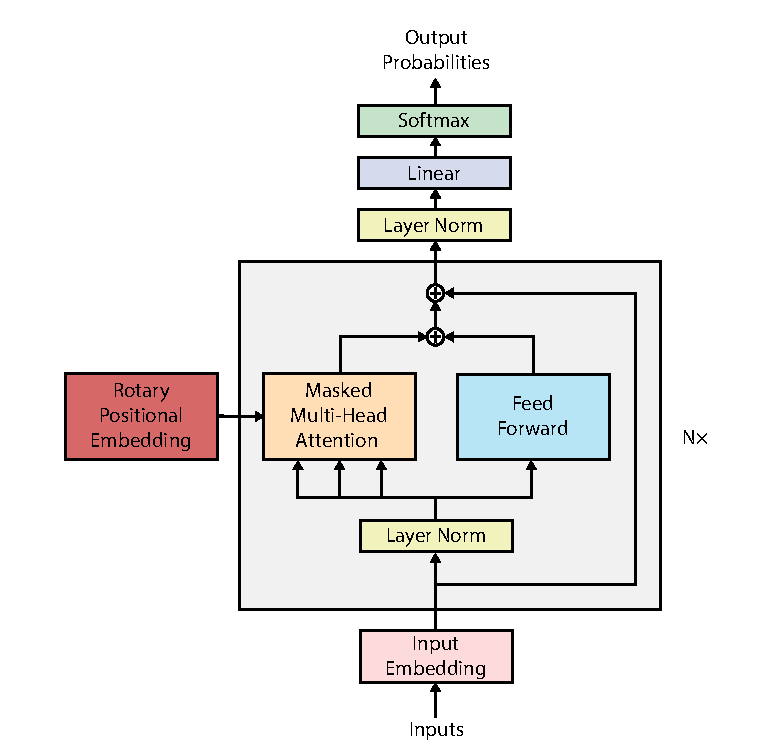
\includegraphics[width=0.8\textwidth]{figures/gpt-j_architecture.pdf}
    \caption{Diagram of GPT-J model architecture}
    \label{fig:gpt-j-architecture}
\end{figure}

\subsection{Requirements}
\label{sec:requirements}
To load the GPT-J model in float32 precision, one would need at least 2x the model size of CPU RAM: 1x for the initial weights and another 1x to load the checkpoint. So for just loading the GPT-J model, it would require at least 48GB or CPU RAM. To reduce the memory footprint, one can load the model in half-precision.

GPU needs around 40GB of GPU memory to load the model. For training/fine-tuning the model, it would require significantly more GPU RAM. For example, the Adam optimizer makes four copies of the model: model, gradients, average and the squared average of gradients. Hence, it would take 4x model size GPU memory, even with mixed precision as gradient updates are in fp32. Further, this doesn't include the activations and data batches which would require some more GPU RAM. Hence, solutions like DeepSpeed needs to be used for training/fine-tuning such large models.

If a GPU with mixed precision capabilities (architecture Pascal or more recent) is available, one can use mixed precision training with PyTorch 1.6.0 or later, or by installing the Apex library for previous versions. If using an NVIDIA “Ampere” GPU architecture, the Brain Floting Point (BF16) floating-point format can be used. Using mixed precision training usually results in 2x-speedup for training with the same final results.

\subsection{Pre-training}
\label{sec:pretraining}
Pre-training is defined as "Training in advanced". By first training the model on a huge dataset, the model can then be fine-tuned on a much smaller dataset. This is so-called transfer learning. In this project, pre-trained weights for GPT-J-6B from ElutherAI are used. The pre-training by ElutherAI is done on the dataset The Pile, described in \cref{sec:the-pile}. Of the roughly 825GiB, 95.16 GiB (7.59\%) of The Pile is code from GitHub. Compared to many other open-source models, GPT-J-6B is one of the most promising models for the task of code generation.

The specific GPT-J model configuration can be seen in \cref{tab:gpt-j-model-details}. In detail, GPT-J-6B consists of 28 layers with a model dimension of 4096, and a feedforward dimension of 16384. The model dimension is split into 16 heads, each with a dimension of 256. \acrfull{rope} is applied to 64 dimensions of each head. The model is trained with a tokenization vocabulary of 50257, using the same set of \acrfullpl{bpe} as GPT-2 and GPT-3. The weights of GPT-J-6B are licensed under version 2.0 of the Apache License.


%Total params: 6,050,882,784
%multi-layer perceptron (MLP)

\begin{table}
    %\newcolumntype{Y}{>{\centering\arraybackslash}X}
    \def\arraystretch{1.5}
    \small
    \centering
    \caption{GPT-J-6B model details.}
    \label{tab:gpt-j-model-details}
    \begin{tabularx}{\textwidth}{XX}
        \toprule
        \textbf{Hyper parameter} & \textbf{Value}\\
        \midrule
        n\_parameters & 6,053,381,344\\
        n\_layers & 28*\\
        d\_model & 4,096\\
        d\_ff & 16,384\\
        n\_heads & 16\\
        d\_head & 256\\
        n\_ctx & 2,048\\
        n\_vocab & 50,257 (same tokenizer as GPT-2/3)\\
        position \& encoding & \acrfullpl{rope}\\
        RoPE dimensions & 64\\
        \bottomrule
    \end{tabularx}
\end{table}

\todo{add table notes}
* each layer consists of one feedforward block and one self attention block


\subsection{Fine-tuning}
\label{sec:fine-tuning}
To improve the pre-trained GPT-J-6B model's smart contract code generation performance, the model is fine-tuned on a dataset only containing real Ethereum Smart Contract code. Specifically, two models are created. The first model, named GPT-J-6B-Smart-Contract, is fine-tuned on the Verified Smart Contracts dataset \cref{sec:verified-smart-contracts}. The other model, named GPT-J-6B-Smart-Contract-Audit, is a secure version of the first model. It is fine-tuned on the Verified Smart Contracts Audit dataset \cref{sec:verified-smart-contracts-audit}, the same dataset as for the first model but with additional labeling from vulnerability analysis.

\begin{table}
    %\newcolumntype{Y}{>{\centering\arraybackslash}X}
    \def\arraystretch{1.5}
    \small
    \centering
    \caption{Hyper parameters for GPT-J model}
    \label{tab:inclusion-exclusion-criteria}
    \begin{tabularx}{\textwidth}{XX}
        \toprule
        \textbf{Hyper parameter} & \\
        \midrule
        \_name\_or\_path & EleutherAI/gpt-j-6B\\
        activation\_function & gelu\_new\\
        architectures & GPTJForCausalLM\\
        attn\_pdrop & 0.0\\
        bos\_token\_id & 50256\\
        embd\_pdrop & 0.0\\
        eos\_token\_id & 50256\\
        gradient\_checkpointing & false\\
        initializer\_range & 0.02\\
        layer\_norm\_epsilon & 1e-05\\
        model\_type & gptj\\
        n\_embd & 4096\\
        n\_head & 16\\
        n\_inner & null\\
        n\_layer & 28\\
        n\_positions & 2048\\
        resid\_pdrop & 0.0\\
        rotary & true\\
        rotary\_dim & 64\\
        scale\_attn\_weights & true\\
        summary\_activation & null\\
        summary\_first\_dropout & 0.1\\
        summary\_proj\_to\_labels & true\\
        summary\_type & cls\_index\\
        summary\_use\_proj & true\\
        tie\_word\_embeddings & false\\
        tokenizer\_class & "GPT2Tokenizer"\\
        transformers\_version & "4.19.0.dev0"\\
        use\_cache & true\\
        vocab\_size & 50400\\
        \bottomrule
    \end{tabularx}
\end{table}


\begin{table}
    %\newcolumntype{Y}{>{\centering\arraybackslash}X}
    \def\arraystretch{1.5}
    \small
    \centering
    \caption{DeepSpeed Zero config.}
    \label{tab:inclusion-exclusion-criteria}
    \begin{tabularx}{\textwidth}{XX}
        \toprule
        \textbf{Hyper parameter} & \\
        \midrule
        stage & 2\\
        contiguous\_gradients & true\\
        reduce\_scatter & true\\
        reduce\_bucket\_size & 2.000000e+08\\
        allgather\_partitions & true\\
        allgather\_bucket\_size & 2.000000e+08\\
        overlap\_comm & true\\
        load\_from\_fp32\_weights & true\\
        elastic\_checkpoint & false\\
        offload\_param & null\\
        \midrule
        offload\_optimizer & device: null\\
        & nvme\_path: null\\
        & buffer\_count: 4\\
        & pin\_memory: false\\
        & pipeline\_read: false\\
        & pipeline\_write: false\\
        & fast\_init: false\\
        \midrule
        sub\_group\_size & 1.000000e+09\\
        prefetch\_bucket\_size & 5.000000e+07\\
        param\_persistence\_threshold & 1.000000e+05\\
        max\_live\_parameters & 1.000000e+09\\
        max\_reuse\_distance & 1.000000e+09\\
        gather\_16bit\_weights\_on\_model\_save & false\\
        ignore\_unused\_parameters & true\\
        round\_robin\_gradients & false\\
        legacy\_stage1 & false\\
        \bottomrule
    \end{tabularx}
\end{table}

\subsection{Inference}

TODO: What is supported by the model? How much memory to use?
We perform beam search with width of 5 and optimize for accuracy@1


\subsection{Security Conditioning}
\label{sec:security-conditioning}
When training a large language model on several gigabytes of open-source code, it is safe to assume that large portions of this code are not safe and contains vulnerabilities. In the case of Smart Contracts, the vulnerability analysis presented in section \ref{sec:verified-smart-contracts} shows that almost 50\% of deployed Smart Contracts contain at least one high-severity vulnerability. This will result in a biased model that may produce a lot of vulnerable code. This section introduces a technique, named security conditioning, to reduce and mitigate this problem.

Vulnerability analysis is a difficult area. It is especially hard in the area of smart contracts, where the execution environment is not deterministic ????\todo{find correct wording.}... Previous works have tried to classify vulnerable code with large language models without much success \todo{Cite previous works}. In this project, instead of classifying vulnerable code, the goal is to make the model more secure by conditioning it on the presence of vulnerabilities.

The security conditioning is done by appending a special security label to each of the records in the training data. This way, the model can use this token(s) to condition whether to produce safe or vulnerable code. This requires the dataset to first be labeled as secure or vulnerable. For this project, SolidityDetector is used for labeling. Further details on the dataset construction can be found in \cref{sec:verified-smart-contracts-audit}.

\todo{Add example of security conditioning.}